%%%%%%%%%%%%%%%%%%%%%%%%%%%%%%%%%%%%%%%%%%%%%%%%%%%%%%%%%%%%%%%
%% U TEXAS THESIS TEMPLATE
%
% Originally by Keith A. Gillow (gillow@maths.ox.ac.uk), 1997
% Modified by Sam Evans (sam@samuelevansresearch.org), 2007
% Modified by John McManigle (john@oxfordechoes.com), 2015
% Modified by Ulrik Lyngs (ulrik.lyngs@cs.ox.ac.uk), 2018-, for use with R Markdown
% Modified by Nilavra Bhattacharya (nilavra@utexas.edu), 2023-, for use with R Markdown
%
% Nilavra Bhattacharya, 24 Jan 2023: Following previous authors: Ulrik Lyngs and John McManigle, broad permissions are granted to use, modify, and distribute this software
% as specified in the MIT License included in this distribution's LICENSE file.
%
% Ulrik Lyngs, 25 Nov 2018: Following John McManigle, broad permissions are granted to use, modify, and distribute this software
% as specified in the MIT License included in this distribution's LICENSE file.
%
% John commented this file extensively, so read through to see how to use the various options.  Remember that in LaTeX,
% any line starting with a % is NOT executed.

%%%%% PAGE LAYOUT
% The most common choices should be below.  You can also do other things, like replace "a4paper" with "letterpaper", etc.

% 'twoside' formats for two-sided binding (ie left and right pages have mirror margins; blank pages inserted where needed):
%\documentclass[a4paper,twoside]{templates/ociamthesis}
% Specifying nothing formats for one-sided binding (ie left margin > right margin; no extra blank pages):
%\documentclass[a4paper]{ociamthesis}
% 'nobind' formats for PDF output (ie equal margins, no extra blank pages):
%\documentclass[a4paper,nobind]{templates/ociamthesis}

% As you can see from the line below, oxforddown uses the a4paper size, 
% and passes in the binding option from the YAML header in index.Rmd:
\documentclass[letterpaper, nobind]{templates/ociamthesis}


%%%%% ADDING LATEX PACKAGES

% hyphenate monospace texttt properly
\usepackage[htt]{hyphenat}

% handle long urls
\usepackage{xurl}

% change the default coloring of links to something sensible
% NB: no need to import xcolor again; already imported in .cls file
% \usepackage[dvipsnames]{xcolor}

% single double and other spacing
\usepackage{setspace}

% ----- BENGALI FONTS --- 
% need to put them before call to fontenc in .cls file
% otherwise chapter headings will look odd
% because fontenc uses the EU encodings
% whereas fontspec automatically includes newer UTF-8 encodings

% add hyperref package with options from YAML %
\usepackage[pdfpagelabels]{hyperref}

\hypersetup{
    colorlinks=true,
    linkcolor=BlueViolet, %Mulberry,
    urlcolor=blue,
    linktoc=all,
    pdftitle={LongSAL: A Longitudinal Search as Learning Study With University Students},
    pdfauthor={Nilavra Bhattacharya নীলাভ্র ভট্টাচার্য্য},
    % pdfpagemode=Bookmarks,
    % filecolor=magenta,
    % citecolor=blue, % not necessary; pandoc is not using \cite{}, it is converting citations to hyperlinks
}

% % \definecolor{mylinkcolor}{RGB}{0,0,139}
% % % \definecolor{myurlcolor}{RGB}{0,0,139}
% % % \definecolor{mycitecolor}{RGB}{197,75,140}
% 
% % \hypersetup{
%   hidelinks,
%   colorlinks,
%   linktoc=all,
%   % linktocpage=true,
%   linkcolor=mylinkcolor,
%   urlcolor=myurlcolor,
%   citecolor=mycitecolor
% }
% 

% add float package to allow manual control of figure positioning %
\usepackage{float}

% enable strikethrough
\usepackage[normalem]{ulem}

% use soul package for correction highlighting
\usepackage{color, soulutf8}
\definecolor{correctioncolor}{HTML}{CCCCFF}
\sethlcolor{correctioncolor}
\newcommand{\ctext}[3][RGB]{%
  \begingroup
  \definecolor{hlcolor}{#1}{#2}\sethlcolor{hlcolor}%
  \hl{#3}%
  \endgroup
}
% stop soul from freaking out when it sees citation commands
\soulregister\ref7
\soulregister\cite7
\soulregister\citet7
\soulregister\autocite7
\soulregister\textcite7
\soulregister\pageref7

%%%%% FIXING / ADDING THINGS THAT'S SPECIAL TO R MARKDOWN'S USE OF LATEX TEMPLATES
% pandoc puts lists in 'tightlist' command when no space between bullet points in Rmd file,
% so we add this command to the template
\providecommand{\tightlist}{%
  \setlength{\itemsep}{0pt}\setlength{\parskip}{0pt}}
 
% allow us to include code blocks in shaded environments

% User-included things with header_includes or in_header will appear here
% kableExtra packages will appear here if you use library(kableExtra)
\usepackage{booktabs}
\usepackage{longtable}
\usepackage{array}
\usepackage{multirow}
\usepackage{wrapfig}
\usepackage{float}
\usepackage{colortbl}
\usepackage{pdflscape}
\usepackage{tabu}
\usepackage{threeparttable}
\usepackage{threeparttablex}
\usepackage[normalem]{ulem}
\usepackage{makecell}
\usepackage{xcolor}


%UL set section header spacing
\usepackage{titlesec}
% 
\titlespacing\subsubsection{0pt}{24pt plus 4pt minus 2pt}{0pt plus 2pt minus 2pt}


%UL set whitespace around verbatim environments
\usepackage{etoolbox}
\makeatletter
\preto{\@verbatim}{\topsep=0pt \partopsep=0pt }
\makeatother


%%%%%%% PAGE HEADERS AND FOOTERS %%%%%%%%%
\usepackage{fancyhdr}
\setlength{\headheight}{15pt}
\fancyhf{} % clear the header and footers
\pagestyle{fancy}
\renewcommand{\chaptermark}[1]{\markboth{\thechapter. #1}{\thechapter. #1}}
\renewcommand{\sectionmark}[1]{\markright{\thesection. #1}} 
\renewcommand{\headrulewidth}{0pt}

\fancyhead[LO]{\emph{\leftmark}} 
\fancyhead[RE]{\emph{\rightmark}} 




% UL page number position 
\fancyfoot[C]{\emph{\thepage}} %regular pages
\fancypagestyle{plain}{\fancyhf{}\fancyfoot[C]{\emph{\thepage}}} %chapter pages




%%%%% SELECT YOUR DRAFT OPTIONS
% This adds a "DRAFT" footer to every normal page.  (The first page of each chapter is not a "normal" page.)

% IP feb 2021: option to include line numbers in PDF

% for line wrapping in code blocks
\usepackage{fancyvrb}
\usepackage{fvextra}
\DefineVerbatimEnvironment{Highlighting}{Verbatim}{breaklines=true, breakanywhere=true, commandchars=\\\{\}}

% This highlights (in blue) corrections marked with (for words) \mccorrect{blah} or (for whole
% paragraphs) \begin{mccorrection} . . . \end{mccorrection}.  This can be useful for sending a PDF of
% your corrected thesis to your examiners for review.  Turn it off, and the blue disappears.
\correctionstrue


%%%%% BIBLIOGRAPHY SETUP
% Note that your bibliography will require some tweaking depending on your department, preferred format, etc.
% If you've not used LaTeX before, I recommend just using pandoc for citations -- this is what's used unless you specific e.g. "citation_package: natbib" in index.Rmd
% If you're already a LaTeX pro and are used to natbib or something, modify as necessary.

% this allows the latex template to handle pandoc citations
\newlength{\cslhangindent}
\setlength{\cslhangindent}{1.5em}
\newlength{\csllabelwidth}
\setlength{\csllabelwidth}{3em}
\newlength{\cslentryspacingunit} % times entry-spacing
\setlength{\cslentryspacingunit}{\parskip}
\newenvironment{CSLReferences}[2] % #1 hanging-ident, #2 entry spacing
 {% don't indent paragraphs
  \setlength{\parindent}{0pt}
  % turn on hanging indent if param 1 is 1
  \ifodd #1
  \let\oldpar\par
  \def\par{\hangindent=\cslhangindent\oldpar}
  \fi
  % set entry spacing
  \setlength{\parskip}{1mm}
  \setlength{\baselineskip}{6mm}
 }%
 {}
\usepackage{calc}
\newcommand{\CSLBlock}[1]{#1\hfill\break}
\newcommand{\CSLLeftMargin}[1]{\parbox[t]{\csllabelwidth}{#1}}
\newcommand{\CSLRightInline}[1]{\parbox[t]{\linewidth - \csllabelwidth}{#1}\break}
\newcommand{\CSLIndent}[1]{\hspace{\cslhangindent}#1}




% Uncomment this if you want equation numbers per section (2.3.12), instead of per chapter (2.18):
%\numberwithin{equation}{subsection}


%%%%% THESIS / TITLE PAGE INFORMATION
% Everybody needs to complete the following:
\title{LongSAL: A Longitudinal Search as Learning Study With University Students}
\author{Nilavra Bhattacharya}


% Master's candidates who require the alternate title page (with candidate number and word count)
% must also un-comment and complete the following three lines:

% Uncomment the following line if your degree also includes exams (eg most masters):
%\renewcommand{\submittedtext}{Submitted in partial completion of the}
% Your full degree name.  (But remember that DPhils aren't "in" anything.  They're just DPhils.)
\degree{Doctor of Philosophy}

% Term and year of submission, or date if your board requires (eg most masters)



%%%%% YOUR OWN PERSONAL MACROS
% This is a good place to dump your own LaTeX macros as they come up.

% To make text superscripts shortcuts
\renewcommand{\th}{\textsuperscript{th}} % ex: I won 4\th place
\newcommand{\nd}{\textsuperscript{nd}}
\renewcommand{\st}{\textsuperscript{st}}
\newcommand{\rd}{\textsuperscript{rd}}

%%%%% THE ACTUAL DOCUMENT STARTS HERE
\begin{document}

%%%%% CHOOSE YOUR LINE SPACING HERE
% This is the official option.  Use it for your submission copy and library copy:
\setlength{\textbaselineskip}{22pt plus2pt}
% This is closer spacing (about 1.5-spaced) that you might prefer for your personal copies:
%\setlength{\textbaselineskip}{18pt plus2pt minus1pt}

% You can set the spacing here for the roman-numbered pages (acknowledgements, table of contents, etc.)
\setlength{\frontmatterbaselineskip}{17pt plus1pt minus1pt}

% UL: You can set the line and paragraph spacing here for the separate abstract page to be handed in to Examination schools
\setlength{\abstractseparatelineskip}{13pt plus1pt minus1pt}
\setlength{\abstractseparateparskip}{0pt plus 1pt}

% UL: You can set the general paragraph spacing here - I've set it to 2pt (was 0) so
% it's less claustrophobic
\setlength{\parskip}{2pt plus 1pt}

%
% Customise title page
%
\def\crest{}
\renewcommand{\university}{The University of Texas at Austin}
\renewcommand{\submittedtext}{}
\renewcommand{\thesistitlesize}{\fontsize{22pt}{28pt}\selectfont}
\renewcommand{\gapbeforecrest}{25mm}
\renewcommand{\gapaftercrest}{25mm
}


% Leave this line alone; it gets things started for the real document.
\setlength{\baselineskip}{\textbaselineskip}


%%%%% CHOOSE YOUR SECTION NUMBERING DEPTH HERE
% You have two choices.  First, how far down are sections numbered?  (Below that, they're named but
% don't get numbers.)  Second, what level of section appears in the table of contents?  These don't have
% to match: you can have numbered sections that don't show up in the ToC, or unnumbered sections that
% do.  Throughout, 0 = chapter; 1 = section; 2 = subsection; 3 = subsubsection, 4 = paragraph...

% The level that gets a number:
\setcounter{secnumdepth}{4}
% The level that shows up in the ToC:
\setcounter{tocdepth}{4}


%%%%% ABSTRACT SEPARATE
% This is used to create the separate, one-page abstract that you are required to hand into the Exam
% Schools.  You can comment it out to generate a PDF for printing or whatnot.

% JEM: Pages are roman numbered from here, though page numbers are invisible until ToC.  This is in
% keeping with most typesetting conventions.
\begin{romanpages}

% Title page is created here
% original code:
% \maketitle

% --------- start: UTexas Frontmatter (committee membership, title page) -------

% ~~~~ committee membership page ~~~~
\thispagestyle{empty} % to not show roman page numbers
\begin{center}
  The Dissertation Committee for Nilavra Bhattacharya\\
  certifies that this is the approved version of the following Dissertation:\\
  \vspace*{30pt}
  \begin{spacing}{2}
    {\Large{\textbf{LongSAL: A Longitudinal Search as Learning Study With University Students}}}
  \end{spacing}
\end{center}

\vspace*{55pt}

\phantom{x}\hspace{45ex} {\large{\textbf{Committee:}}}\\
% \vspace*{12pt}

\begin{flushright}
  Jacek Gwizdka, Supervisor\\
  \vspace*{24pt}
  Soo Young Rieh\\
  \vspace*{24pt}
  Matthew Lease\\
  \vspace*{24pt}
  Robert Capra
\end{flushright}


% ~~~~ title page ~~~~
\newpage
\thispagestyle{empty} % to not show roman page numbers
\begin{center}
  
  \begin{spacing}{2}
    {\Large{\textbf{LongSAL: A Longitudinal Search as Learning Study With University Students}}}
  \end{spacing}
  
  \vspace*{24pt}

  \begin{spacing}{1.4}
    by\\
    
    \vspace*{24pt}
    
    {\Large{\textbf{
      Nilavra Bhattacharya\\
      \vspace*{10pt}
      {\Huge {\secondlanguage নীলাভ্র ভট্টাচার্য্য}}
    }}}
    
    \vspace*{72pt}
    
    {\Large{\textbf{Dissertation}}}\\
    
    \vspace*{24pt}
    
    Presented to the Faculty of the Graduate School\\
    of The University of Texas at Austin\\
    in Partial Fulfillment\\
    of the Requirements\\
    for the Degree of\\
    
    \vspace*{30pt}
    
    {\Large{\textbf{Doctor of Philosophy}}}\\
    
    \vfill

    {\large{The University of Texas at Austin\\
    August 2023}}

  \end{spacing}
\end{center}


% --------- end: UTexas Frontmatter (committee membership, title page) -------


%%%%% DEDICATION

%%%%% ACKNOWLEDGEMENTS


\begin{acknowledgements}
 	This section will be fleshed out in more detail after the initial submission. For now, I wish to thank the following people :

 PhD Committee Members: Professors

 \begin{itemize}
 \tightlist
 \item
   Jacek Gwizdka (chair)
 \item
   Soo Young Rieh
 \item
   Matt Lease
 \item
   Rob Capra (UNC Chapel Hill, USA)
 \end{itemize}

 Mentors from CHIIR 2021 Doctoral Colloquium: Professors

 \begin{itemize}
 \tightlist
 \item
   Pertti Vakkari (Tampere Univerisity, Finland)
 \item
   Ian Ruthven (University of Strathclyde, UK)
 \item
   Gerd Berget (Oslo Metropolitan University, Norway)
 \end{itemize}
\end{acknowledgements}



%%%%% ABSTRACT



% --------- start: UTexas abstract -------
\begin{center}
  \textbf{Abstract}\\
  
  \vspace{18pt}
  
  % title
  \begin{spacing}{2}
    {\Large{\textbf{LongSAL: A Longitudinal Search as Learning Study With University Students}}}
  \end{spacing}

  \vspace{18pt}

  % author + supervisor
  \begin{spacing}{1.4}
    % Nilavra Bhattacharya নীলাভ্র ভট্টাচার্য্য, PhD\\
    Nilavra Bhattacharya 
    {\secondlanguage নীলাভ্র ভট্টাচার্য্য}, 
    PhD\\
    The University of Texas at Austin, 
    2023\\
    \vspace{18pt}
    Supervisor: Jacek Gwizdka
  \end{spacing}

\end{center}

\begin{spacing}{1.5}
  \indent
  % \indent
  Learning today comprises navigation, discernment, induction, and synthesis of the wide body of information on the Internet present ubiquitously at every student's fingertips.
  Learning, or addressing a gap in one's knowledge, has been well established as an important motivator behind information-seeking activities.
  The Search as Learning research community advocates that online information search systems should be reconfigured to become educational platforms to foster learning and \emph{sensemaking}.
  Modern search systems have yet to adapt to support this function.
  An important step to foster learning during online search is to identify behavioural patterns that distinguish searchers gaining more vs.~less knowledge during search.
  Previous efforts have primarily studied searchers in the short term, typically during a single lab session.
  Researchers have expressed concerns over this ephemeral approach, as learning takes place over time, and is not fleeting.
  In this dissertation, an exploratory longitudinal study was conducted to observe the long-term searching behaviour of students enrolled in a university course, over the span of a semester.
  Our research aims were to identify if and how students' searching behaviour changes over time, as they gain new knowledge on a subject; and how do individual traits such as motivation, metacognition, self-regulation, and other individual differences moderate their searching as learning behaviour.
  We found that differences in these traits do create observable and quantifiable differences in information searching as a learning activity.
  Students with higher levels of these traits were more effective and efficient in their search behaviours, reported better levels of learning and search outcomes, and obtained better grades.
  We posit that learning environments should be designed to foster the effective use of metacognitive strategies to help learners develop and apply productive self-regulated learning.
  Moreover, learning technologies can be used to induce, track, model, and support learners' metacognition across tasks, domains, and contexts.
  The study recommends that understanding the complex relationship between motivation and metacognition is essential to designing effective searching as learning environments.
  Findings from this exploratory longitudinal study will help to build improved search systems that foster human learning and sensemaking, which are more equitable in the face of learner diversity.
\end{spacing}

% --------- end: UTexas abstract -------

% --------- start: UTexas abstract 2nd language -------
\newpage
\begin{center}
  \textbf{\secondlanguage{সারসংক্ষেপ} (Abstract in Bengali)}\\
  
  \vspace{18pt}
  
  % title
  \begin{spacing}{2}
    \secondlanguage{\Large{\textbf{লংস্যাল: ইন্টারনেটে তথ্য অনুসন্ধানের মাধ্যমে শিক্ষার্থীদের জ্ঞানলাভ বোঝার জন্য একটি অনুদৈর্ঘ্য গবেষণা}}}
  \end{spacing}

  \vspace{18pt}

  % author + supervisor
  \begin{spacing}{1.4}
    % Nilavra Bhattacharya নীলাভ্র ভট্টাচার্য্য, PhD\\
    % Nilavra Bhattacharya 
    \secondlanguage{নীলাভ্র ভট্টাচার্য্য}, 
    PhD\\
    টেক্সাস বিশ্ববিদ্যালয়, অস্টিন, মার্কিন যুক্তরাষ্ট্র, 
    শ্রাবণ ১৪৩০ (আগস্ট ২০২৩)\\
    \vspace{18pt}
    সুপারভাইজার: ইয়াৎসেক গুইজদকা
  \end{spacing}

\end{center}

\begin{spacing}{1.5}
  \indent
  % \indent
  \secondlanguage{Bengali version of abstract: TBD.
আমার পিএইচডি এডভাইসর পরামর্শ দিয়েছেন যে এই থিসিস এর একটি বাংলা ভাসায় সারসংক্ষেপ ও লিখতে। উনি ওনার থিসিস এর সারসংক্ষেপ ইংরেজি এবং পোলিশ দুই ভাষায় লিখেছিলেন।
থিসিসের প্রথম খসড়া জমা দেওয়ার পরে বাংলা সারসংক্ষেপ টি আরও বিস্তারিতভাবে লেখা হবে।
বাংলা সংস্করণ এর উৎসর্গ: দিদার জন্য.
Bengali version of abstract: TBD.

বর্তমান যুগে শিক্ষার একটা বড় অংশ হলো ইন্টারনেটের বিপুল তথ্যের ভাণ্ডার -- যা প্রায় প্রতিটি ছাত্রের নখদর্পণে সর্বব্যাপী উপস্থিত -- সেই তথ্যের ভাণ্ডারে অনুসন্ধান করা, উপযুক্ত তথ্য সংগ্রহণ করা, এবং সংগৃহীত তথ্যের বিশ্লেষণ করা।
শিক্ষা, বা জ্ঞানের শূন্যস্থান পূরণ করা তথ্য অনুসন্ধানের একটি গুরুত্বপূর্ণ কারণ হিসাবে প্রতিষ্ঠিত।
``Search as Learning'' বা ``অনুসন্ধানের মাধ্যমে শিক্ষা'' -- এই সম্প্রদায়ের গবেষকরা মনে করেন যে বর্তমান ``সার্চ ইঞ্জিন'' বা

বাংলা অনুবাদের জন্য বিশেষ কৃতজ্ঞতা স্বীকার : আসিফ শাহরিয়ার
জার্মানির হামবুর্গ শহরে CHI ২০২৩ সম্মেলনে ওনার সাথে আমার পরিচয়}
\end{spacing}

% --------- end: UTexas abstract 2nd language -------



%%%%% MINI TABLES
% This lays the groundwork for per-chapter, mini tables of contents.  Comment the following line
% (and remove \minitoc from the chapter files) if you don't want this.  Un-comment either of the
% next two lines if you want a per-chapter list of figures or tables.
\dominitoc % include a mini table of contents

% This aligns the bottom of the text of each page.  It generally makes things look better.
\flushbottom

% This is where the whole-document ToC appears:
\tableofcontents

\listoffigures
	\mtcaddchapter
  	% \mtcaddchapter is needed when adding a non-chapter (but chapter-like) entity to avoid confusing minitoc

% Uncomment to generate a list of tables:
%%%%% LIST OF ABBREVIATIONS
% This example includes a list of abbreviations.  Look at text/abbreviations.tex to see how that file is
% formatted.  The template can handle any kind of list though, so this might be a good place for a
% glossary, etc.

% The Roman pages, like the Roman Empire, must come to its inevitable close.
\end{romanpages}

%%%%% CHAPTERS
% Add or remove any chapters you'd like here, by file name (excluding '.tex'):
\flushbottom

% all your chapters and appendices will appear here
\hypertarget{introduction}{%
\chapter{Introduction}\label{introduction}}

\hypertarget{sec-intro-overview}{%
\section{Searching as Learning: Overview}\label{sec-intro-overview}}

Searching for information is a fundamental human activity. In the modern world, it is frequently conducted by users interacting with online search systems (e.g., web search engines), or more formally, \textbf{Information Retrieval} (IR) systems.
As early as in 1980, Bertam Brookes, in his `fundamental equation' of information and knowledge, had stated that an information searcher's current state of knowledge is changed to a new knowledge structure by exposure to information (\protect\hyperlink{ref-brookes1980foundations}{Brookes, 1980, p. 131}).
This indicates that searchers acquire new knowledge in the search process, and the same information will have different effects on different searchers' knowledge states.
Fifteen years later, Marchionini (\protect\hyperlink{ref-marchionini1995information}{1995}) described information seeking as ``a process, in which humans purposefully engage in order to change
their state of knowledge''.
Thus, we have known for quite a while that search is driven by higher-level human needs, and IR systems are a means to an end, and not the end in itself.
\textbf{Interactive information retrieval} (IIR), a.k.a. human-computer information retrieval (HCIR) (\protect\hyperlink{ref-marchionini2006toward}{Marchionini, 2006}) refers to the study and evaluation of users' interaction with IR systems and users' satisfaction with the retrieved information (\protect\hyperlink{ref-borlund2013interactive}{Borlund, 2013}).

Despite their technological marvels, modern IR systems falls short in several aspects of fully satisfying the higher level human need for information.
In essence, IR systems are software that take, as input, some query, and return as output some ranked list of resources.

\begin{quote}
\emph{Within the context of information seeking, (search engines and IR systems) \textbf{feel} like they play a prominent role in our lives, when in actuality, they only play a small role: the \textbf{retrieval} part of information \ldots{}}

\begin{itemize}
\item
  \emph{Search engines \textbf{don't help us identify what we need} -- that's up to us; search engines don't question what we ask for, though they do recommend queries that use similar words.}
\item
  \emph{Search engines \textbf{don't help us choose a source} -- though they are themselves a source, and a heavily marketed one, so we are certainly compelled to choose search engines over other sources, even when other sources might have better information.}
\item
  \emph{Search engines \textbf{don't help us express our query} accurately or precisely -- though they will help with minor spelling corrections.}
\item
  \emph{Search engines do help retrieve information---this is the primary part that they automate.}
\item
  \emph{Search engines \textbf{don't help us evaluate the answers we retrieve} -- it's up to us to decide whether the results are relevant, credible, true; Google doesn't view those as their responsibility.}
\item
  \emph{Search engines \textbf{don't help us sensemake} -- we have to use our minds to integrate what we've found into our knowledge.}
\end{itemize}

\hfill --- Ko (\protect\hyperlink{ref-ko2021seeking}{2021})
\end{quote}

In recent years, the IIR research community has been actively promoting the \textbf{Search as Learning} (SAL) research direction.
This fast-growing community of researchers propose that search environments should be augmented and reconfigured to foster learning, sensemaking, and long-term knowledge-gain.
Various workshops and seminars have been organized to develop research agendas at the interaction of IIR and the Learning Sciences (\protect\hyperlink{ref-agosti2014evaluation}{Agosti et al., 2014}; \protect\hyperlink{ref-allan2012frontiers}{Allan et al., 2012}; \protect\hyperlink{ref-collins2017search}{Collins-Thompson et al., 2017}; \protect\hyperlink{ref-freund2013searching}{Freund et al., 2013}, \protect\hyperlink{ref-freund2014searching}{2014}; \protect\hyperlink{ref-gwizdka2016search}{Gwizdka et al., 2016}).
Additionally, special issues on Search as Learning have also been published in the \emph{Journal of Information Science} (\protect\hyperlink{ref-hansen2016editorial}{Hansen \& Rieh, 2016}) and in the \emph{Information Retrieval Journal} (\protect\hyperlink{ref-eickhoff2017introduction}{Eickhoff et al., 2017}).
Articles in these special issued presented landmark literature reviews (\protect\hyperlink{ref-rieh2016searching}{Rieh et al., 2016}; \protect\hyperlink{ref-vakkari2016searching}{Vakkari, 2016}), research agendas, and ideas
in this direction.
Overall, these works generally advocate that future research in this domain should aim to:

\begin{itemize}
\tightlist
\item
  understand the contexts in which people search to learn
\item
  understand factors that can influence learning outcomes
\item
  understand how search behaviours can predict learning outcomes
\item
  develop search systems to better support learning and sensemaking
\item
  help searchers be more critical consumers of information
\item
  understand the cognitive biases fostered by existing search systems
\item
  develop search engine ranking algorithms and interface tools that foster long term knowledge gain
\end{itemize}

Parallelly, the Educational Science and the Learning Science research communities have also been organizing workshops and formulating research
agendas to conceptualize forms of `new learning' (\protect\hyperlink{ref-cope2013new}{Cope \& Kalantzis, 2013}; \protect\hyperlink{ref-kalantzis2012newa}{Kalantzis \& Cope, 2012}; \protect\hyperlink{ref-newlondon1996pedagogy}{New London Group, 1996}) that are afforded by innovations in digital technologies and e-learning ecologies (\protect\hyperlink{ref-cope2017elearningc}{Cope \& Kalantzis, 2017}).
Higher education researchers have been increasingly studying how students' information search and information use behaviour affect and support their learning (\protect\hyperlink{ref-weber2018can}{Weber et al., 2018}, \protect\hyperlink{ref-weber2019informationseeking}{2019}; \protect\hyperlink{ref-zlatkin2021students}{Zlatkin-Troitschanskaia et al., 2021}).
Efforts are underway to conceptualize a theoretical framework around new forms of e-Learning that is aided and afforded by digital technologies (\protect\hyperlink{ref-amina2017active}{Amina, 2017}; \protect\hyperlink{ref-cope2017elearningc}{Cope \& Kalantzis, 2017}).
In the community's own words: ``learning today is more about navigation, discernment, induction, and synthesis'' of the wide body of information present ubiquitously at every student's fingertips (\protect\hyperlink{ref-amina2017active}{Amina, 2017}).
Therefore, ``knowing the source, finding the source, and using the information aptly is important to learn and know now more than ever before'' (\protect\hyperlink{ref-cope2013new}{Cope \& Kalantzis, 2013}).
All of these interests in the intersection of searching and learning goes to emphasize that understanding learning during search is critical to
improve human-information interaction.

\hypertarget{sec-intro-problem-statement}{%
\section{Problem Statement}\label{sec-intro-problem-statement}}

A major limitation in the area of Search as Learning, Interactive IR (IIR), and more broadly, in Human-Computer Interaction (HCI) research is
that, the user is examined in the short-term, typically over the course of a single experimental session in a lab
(\protect\hyperlink{ref-karapanos2021advances}{Karapanos et al., 2021}; \protect\hyperlink{ref-kelly2009evaluation}{Kelly et al., 2009}; \protect\hyperlink{ref-koeman2020hciux}{Koeman, 2020}; \protect\hyperlink{ref-zlatkin2021students}{Zlatkin-Troitschanskaia et al., 2021}).
Very few studies exist in the search-as-learning domain that have observed \emph{the same participant} over a longer period of time than a single search session (\protect\hyperlink{ref-kelly2006measuringa}{Kelly, 2006a}, \protect\hyperlink{ref-kelly2006measuringb}{2006b}; \protect\hyperlink{ref-kuhlthau2004seeking}{Kuhlthau, 2004}; \protect\hyperlink{ref-vakkari2001changes}{Vakkari, 2001a}; \protect\hyperlink{ref-white2009characterizing}{White et al., 2009}; \protect\hyperlink{ref-wildemuth2004effects}{Wildemuth, 2004}).
This ephemeral approach has acute implications in any domain where learning is involved because ``learning is a \emph{process} that leads to \emph{change} in knowledge \ldots{} (which) unfolds over time'' (\protect\hyperlink{ref-ambrose2010howa}{Ambrose et al., 2010}), and ``\ldots does not happen all at once'' (\protect\hyperlink{ref-white-2016-iwss-learning}{White, 2016b}).

\textbf{To the best of the author's knowledge, almost no new longitudinal studies were reported in major search-as-learning literature in the last five years, that systematically studied students' information search behaviour and information-use over the long term, in their \emph{in-situ} naturalistic environment and contexts, and linked those behaviours quantitatively to the students' learning outcomes and individual differences.}

Higher education students are increasingly using the Internet as their main learning environment and source of information when studying. Yet, the short term nature of research in this domain creates significant gaps in our knowledge regarding how students' information search behaviour and information use develop over time, and how it affects their learning (\protect\hyperlink{ref-zlatkin2021students}{Zlatkin-Troitschanskaia et al., 2021}).

\begin{quote}
\emph{When research in this area relies so heavily on (short-term) lab studies, can we realistically say we are comprehensively studying human-tech interactions -- when many of those interactions take place over long periods of time in real-world contexts? \ldots{} An over-reliance on short studies risks inaccurate findings, potentially resulting in prematurely embracing or disregarding new concepts.}

\hfill --- Koeman (\protect\hyperlink{ref-koeman2020hciux}{2020})
\end{quote}

Current search engines and information retrieval systems ``do not help us know what we want to know, \ldots do not help us know if what we've found is relevant or true; and they do not help us make sense of the retrieved information.
All they do is quickly retrieve what other people on the internet have shared'' (\protect\hyperlink{ref-ko2021seeking}{Ko, 2021}).
Unless we have more long-term understanding of the nature of knowledge gain during search, the limitations of current search systems will continue to persist.
Increased knowledge and understanding of students', and more broadly searchers', information searching and learning behaviour over time will help us to overcome the limitations of current IR systems, and transform them into rich learning spaces where ``search experiences and learning experiences are intertwined and even synergized'' (\protect\hyperlink{ref-url-rieh-homepage}{Rieh, 2020}).
The internet and digital educational technologies offer great opportunities to transform learning and the education experience.
Enabled by our increased comprehension of the longitudinal searching-as-learning process, improved and validated by empirical data, we can create a new wave of fundamentally transformative educational technologies and ``e-learning ecologies, that will be more engaging for learners, more effective (than traditional classroom practices), more resource efficient, and more equitable in the face of learner diversity'' (\protect\hyperlink{ref-cope2017elearningc}{Cope \& Kalantzis, 2017}).

\hypertarget{sec-intro-purpose}{%
\section{Purpose of this Dissertation}\label{sec-intro-purpose}}

To address the gaps in our knowledge of how information searching influences students' learning process over time, this dissertation conducted a semester-long longitudinal study (approx. 16 weeks) with university student participants.
The overarching research aim is to identify how students' online searching behaviour correlate with their learning outcomes for a particular university course.
Building upon principles from the Learning Sciences (\protect\hyperlink{ref-ambrose2010howa}{Ambrose et al., 2010}; \protect\hyperlink{ref-council2000how}{National Research Council, 2000}; \protect\hyperlink{ref-novak2010learninga}{Novak, 2010}; \protect\hyperlink{ref-sawyer2005cambridge}{Sawyer, 2005}),
and empirical evidences from the Information Sciences (\protect\hyperlink{ref-rieh2016searching}{Rieh et al., 2016}; \protect\hyperlink{ref-vakkari2016searching}{Vakkari, 2016}; \protect\hyperlink{ref-white2016interactions}{White, 2016a}),
this dissertation aimed at:

\begin{itemize}
\tightlist
\item
  situating students as learners in their naturalistic contexts, and characterized by their individual differences
\item
  measuring students' information search and information use behaviour over time
\item
  correlating the information search behaviour with the learning outcomes for the university course
\end{itemize}

Learning, or addressing a gap in one's knowledge, has been well established as an important motivator behind information-seeking activities
Section \ref{sec-intro-overview}.
Therefore, search systems that support rapid learning across a number of searchers, and a range of tasks, can be considered as more effective search systems (\protect\hyperlink{ref-white2016interactions}{White, 2016a, p. 310}).
This dissertation takes a step in this direction.
``It opens great expectations for many-sided, great contribution to our knowledge on the relations between search process and learning outcomes'' (anonymous reviewer for \protect\hyperlink{ref-bhattacharya2021longitudinal}{Bhattacharya, 2021}).

\hypertarget{sec-intro-outline}{%
\section{Outline}\label{sec-intro-outline}}

This dissertation document is structured as follows.
First, principles of learning and relevant background from the domain of Educational Sciences are presented in Chapter 2.
Next, relevant empirical evidences from the Information Searching Literature are discussed in Chapter 3.
Chapter 4 presents the research questions,
and discusses their rationale in the context of
the existing research gaps.
Chapter 5 describes the research methods, specifically the longitudinal study design and experimental procedures.
Chapter 6 and 7 presents the data analyses framework, results, and discussions of the findings the study.
Chapter 8 places the findings in terms of the research questions introduced in Chapter 4.
Finally, Chapter 9 presents the conclusion, limitations, and future work.

\hypertarget{ch-bg-learn}{%
\chapter{Background: Knowledge and Learning}\label{ch-bg-learn}}

This first chapter on background literature discusses relevant concepts
from the disciplines of Education and Learning Sciences. First, we
introduce some relevant terminology, and the concepts of deep or
meaningful learning. Then we discuss several research backed principles
that have been shown to lead to meaningful learning. Next, we discuss
how learning, sensemaking, and searching for information are related,
and how modern technologies provide affordances for new forms of
learning and knowledge work in the 21st century. We also discuss some
concepts about individual differences of learners as well as techniques
that can promote better learning. In the last section, we state what
implications these findings have for shaping the longitudinal study in this
dissertation.

\hypertarget{sec-bg-learn-terminology}{%
\section{Terminology}\label{sec-bg-learn-terminology}}

The Webster dictionary\footnote{\url{https://www.merriam-webster.com/dictionary/knowledge}} defines \textbf{knowledge} in two ways. The first
definition is ``the range of one's information or understanding''.
Vakkari (\protect\hyperlink{ref-vakkari2016searching}{2016}) says it is ``the totality what a person knows,
that is, a \textbf{personal knowledge} or \textbf{belief system}. It may include
both justified, true beliefs and less justified, not so true beliefs,
which the person more or less thinks hold true.'' Webster's second
definition of knowledge is ``the sum of what is known: the body of truth,
information, and principles acquired by humankind''. We can regard this
as \textbf{universal knowledge}.

\textbf{Learning} is a \emph{process}, that leads to a \emph{change} in (personal)
knowledge, beliefs, behaviours, and attitudes (\protect\hyperlink{ref-ambrose2010howa}{Ambrose et al., 2010}). Thus,
learning always aims to increase one's personal knowledge, and can often
draw from the body of universal knowledge. In some cases, the change in
personal knowledge can also lead to change in universal knowledge, such
as when new discoveries are made, or new philosophies are proposed.
Human learning is an innate capacity. It is longitudinal and unfolds
over time. Learning is lifelong and life-wide, and has a lasting impact
on how humans think and act (\protect\hyperlink{ref-ambrose2010howa}{Ambrose et al., 2010}; \protect\hyperlink{ref-kalantzis2012newa}{Kalantzis \& Cope, 2012}).
Learning can be informal or formal. \textbf{Informal learning} is the casual
learning taking place in everyday life, and is incidental to the
everyday life experience. \textbf{Formal learning} is the deliberate,
conscious, systematic, and explicit acquiring of knowledge
(\protect\hyperlink{ref-kalantzis2012newa}{Kalantzis \& Cope, 2012}).

\textbf{Education} is a form of formal learning. It is the systematic
acquiring of knowledge. In today's world, the institutions of education
are formally constructed places (classrooms), times (of the day and of
life) and social relations (teachers and students); for instance,
schools, colleges, and universities. The scientific discipline of
Education concerns itself with the systematic investigation of the ways
in which humans know and learn. It is the science of ``coming to know''
(\protect\hyperlink{ref-kalantzis2012newa}{Kalantzis \& Cope, 2012}).

\begin{figure}

{\centering 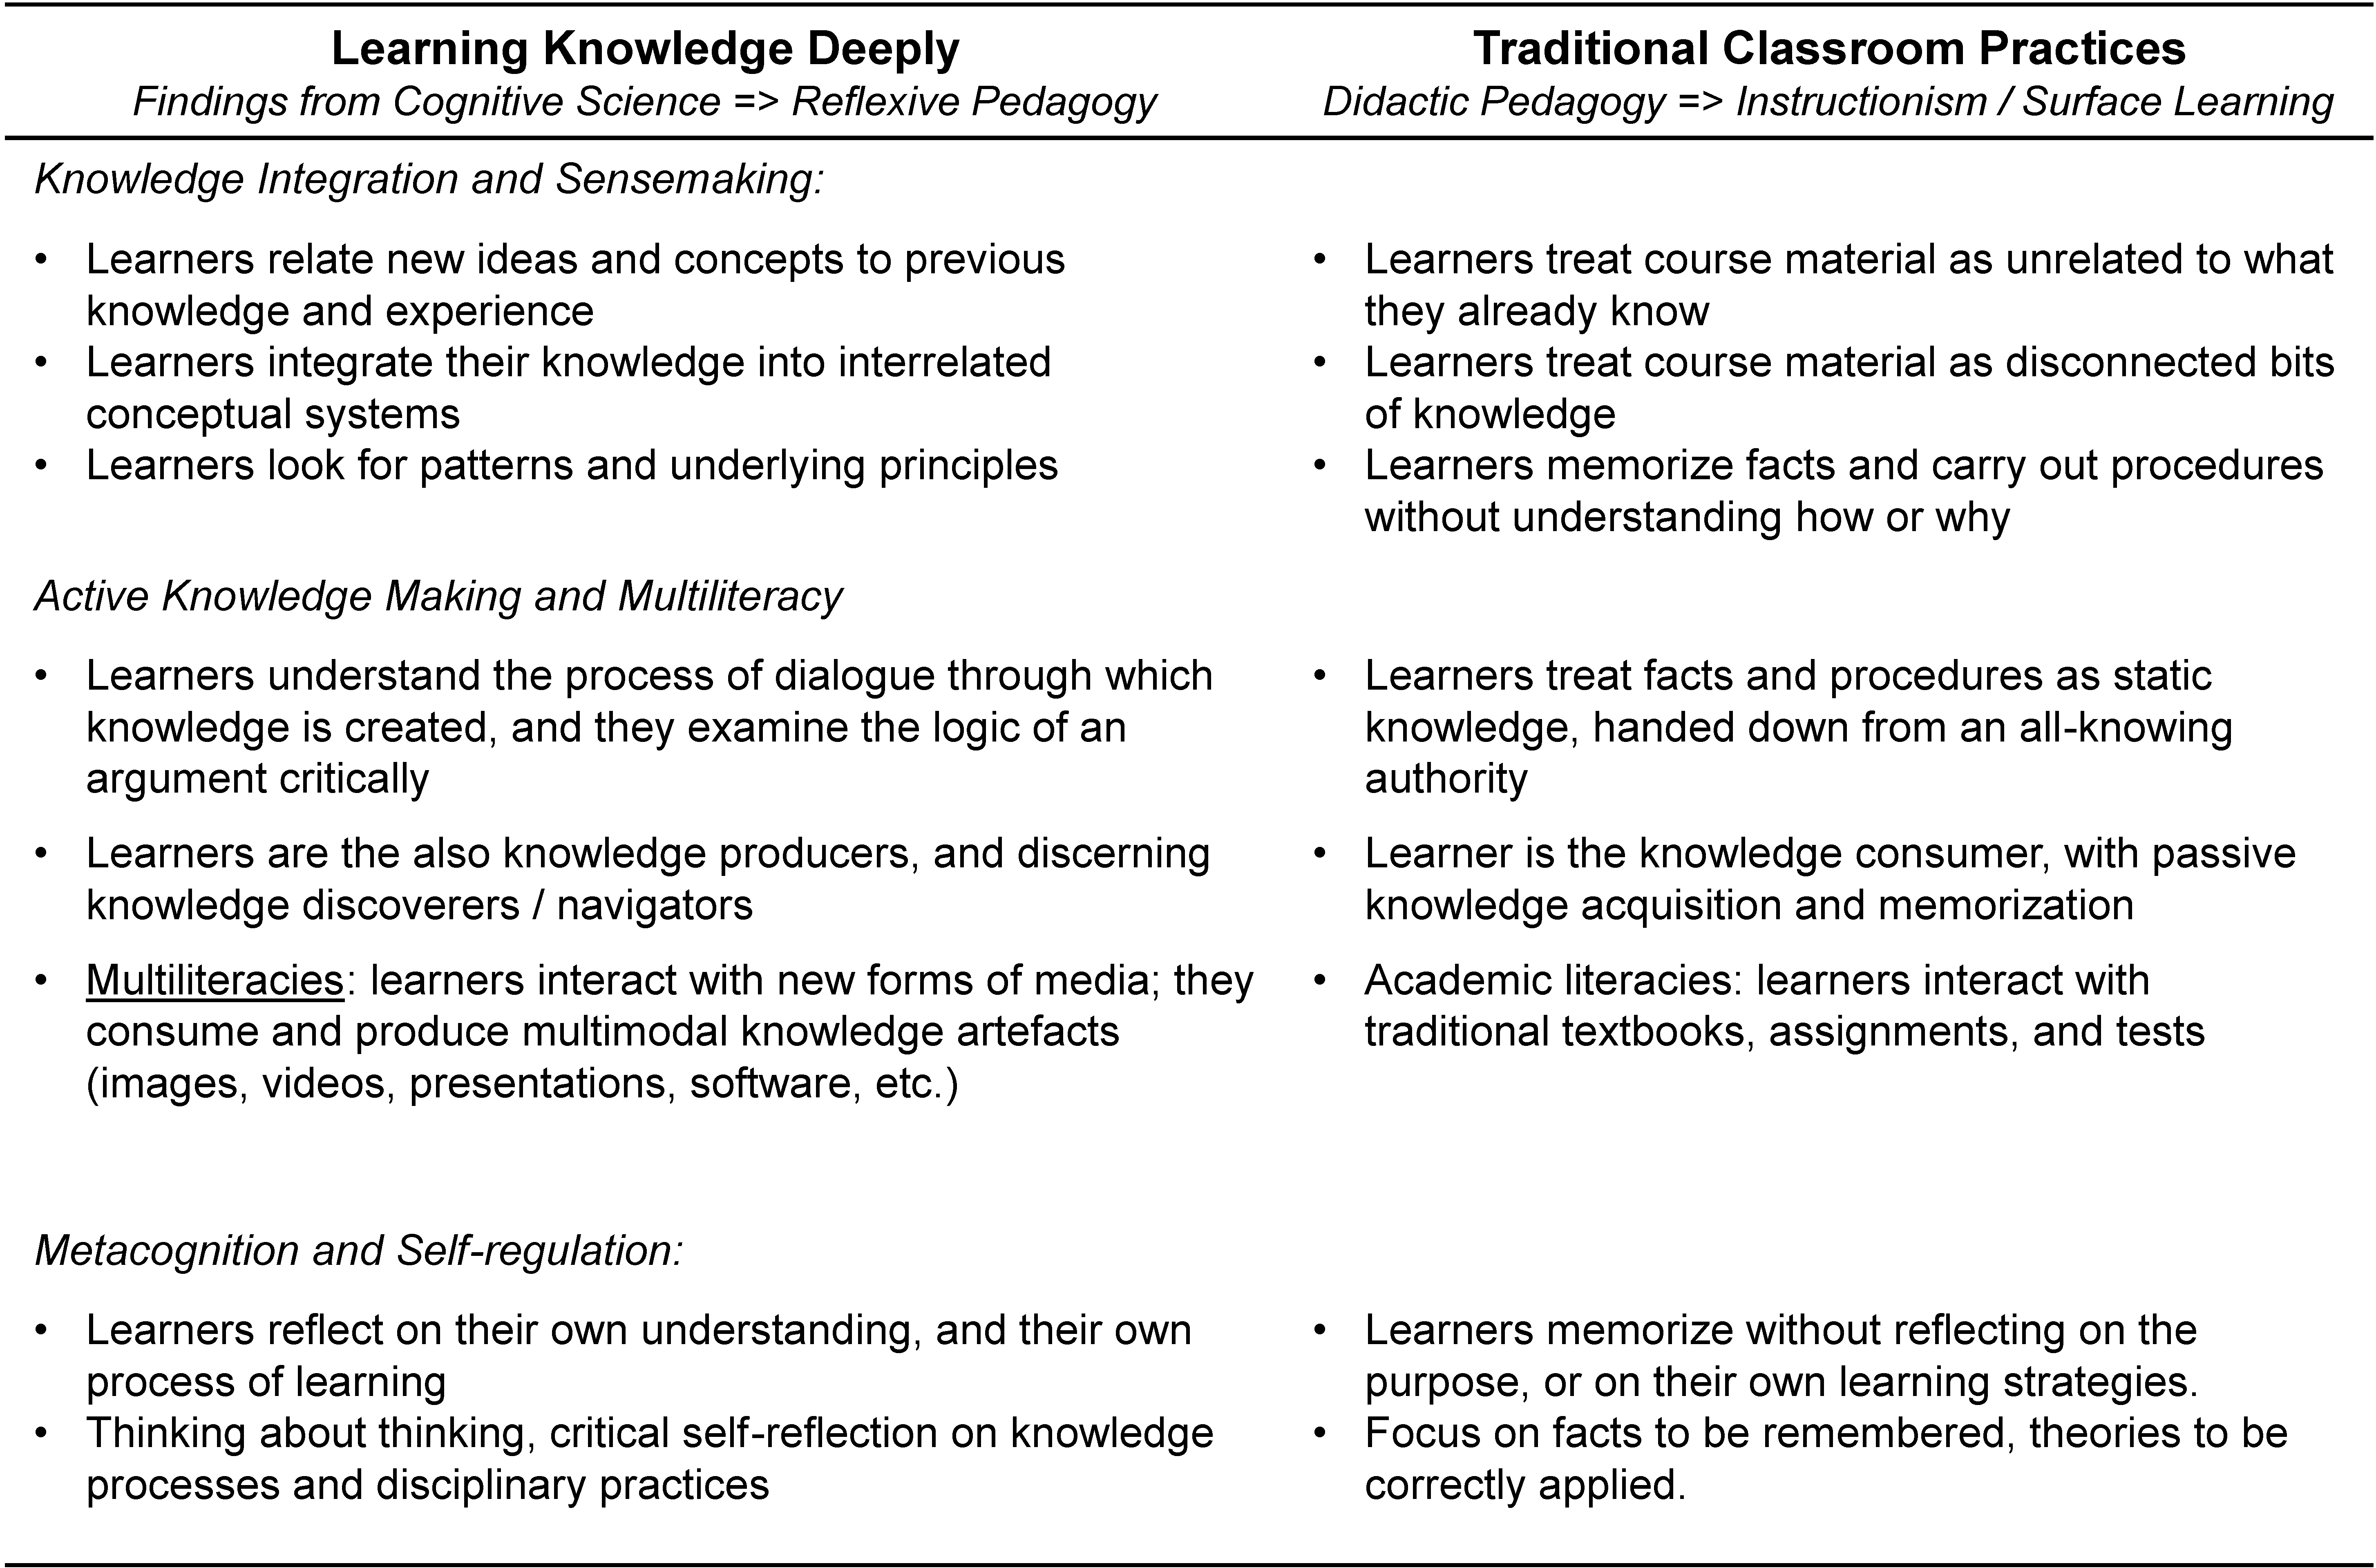
\includegraphics[width=1\linewidth]{figs/deep-learning-surface-learning} 

}

\caption[Learning knowledge deeply vs.~traditional classroom practices.]{Deep learning (of the human kind) versus traditional (also often online) classroom practices. Compiled from Cope \& Kalantzis (\protect\hyperlink{ref-cope2017elearningc}{2017}) and Sawyer (\protect\hyperlink{ref-sawyer2005cambridge}{2005}).}\label{fig:deep-learning-surface-learning}
\end{figure}





\textbf{Pedagogy} describes small sequences of learner activities that
promote learning in educational settings (\protect\hyperlink{ref-kalantzis2012newa}{Kalantzis \& Cope, 2012}).
Traditional approaches to (classroom) pedagogy, especially the \emph{didactic
pedagogy}, primarily involves a teacher telling, and a learner
listening. The teacher is in command of the knowledge, and their mission
is to transmit this knowledge to the learners, in a one-way flow. It is
hoped that the learners will dutifully absorb the knowledge laid before
them by the teacher. The balance of agency weighs heavily towards the
teacher. ``There is a special focus on long-term memory, or retention,
measurable by the ritual of closed-book, summative examination''
(\protect\hyperlink{ref-cope2017elearningc}{Cope \& Kalantzis, 2017}).

\begin{figure}

{\centering 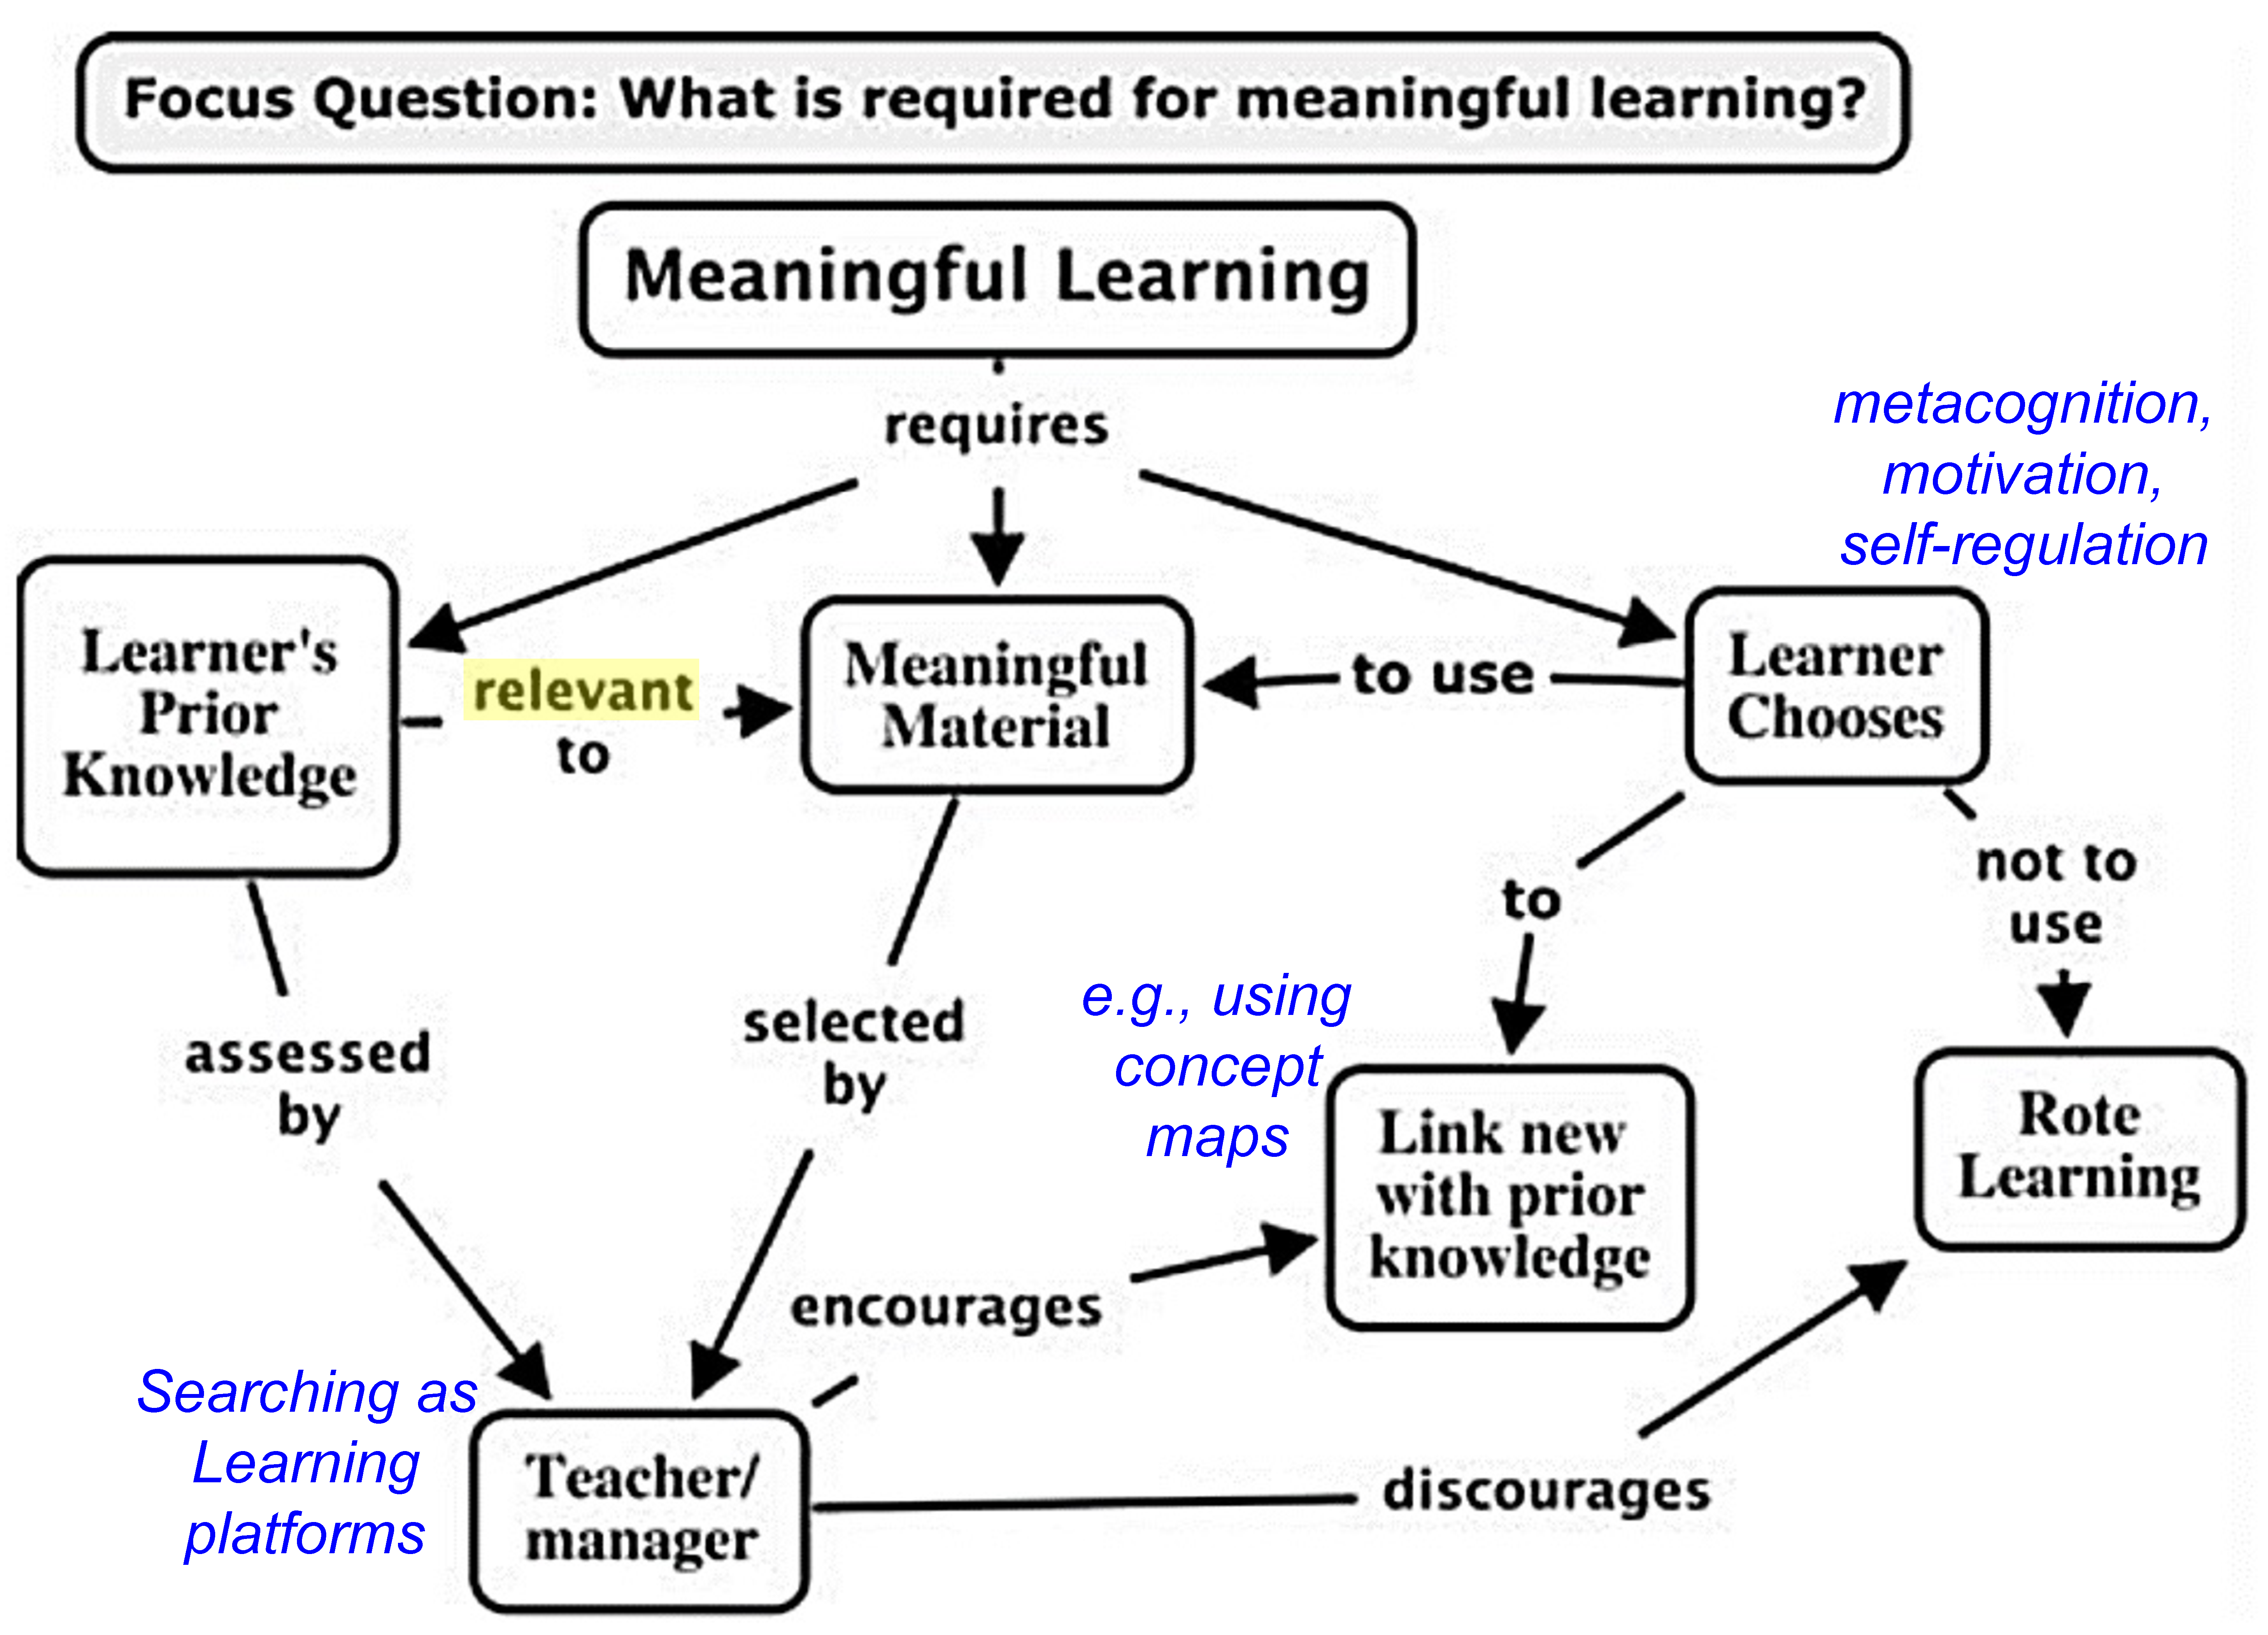
\includegraphics[width=0.7\linewidth]{figs/meaningful-learning} 

}

\caption[Meaningful learning.]{Meaningful learning (aka deep learning) as explained by Novak (\protect\hyperlink{ref-novak2010learninga}{2010, fig. 5.3}) (annotations our own).}\label{fig:meaningful-learning}
\end{figure}





Cognitive scientists had discovered that learners retain material
better, and are able to generalize and apply it to a broader range of
contexts, when they learn \textbf{deep knowledge} rather than \textbf{surface
knowledge}, and when they learn how to use that knowledge in real-world
social and practical settings (\protect\hyperlink{ref-sawyer2005cambridge}{Sawyer, 2005}). Deep learning \footnote{of the human kind} takes place when ``the learner chooses conscientiously to integrate new
knowledge to knowledge that the learner already possesses'' and involves
``substantive, non-arbitrary incorporations of concepts into cognitive
structure'' (\protect\hyperlink{ref-novak2002meaningful}{Novak, 2002, p. 549}) and may eventually lead to the
development of transferable knowledge and skills. A parallel terminology
for deep learning (\protect\hyperlink{ref-marton1976qualitative-b}{Marton \& Säaljö, 1976}; \protect\hyperlink{ref-marton1976qualitative-a}{Marton \& Säljö, 1976})
is \textbf{meaningful learning}
(\protect\hyperlink{ref-ausubel1968educational}{Ausubel et al., 1968}; \protect\hyperlink{ref-novak2002meaningful}{Novak, 2002}), and they are often
contrasted with \emph{surface learning} or \emph{rote learning}.
Figure \ref{fig:deep-learning-surface-learning} discusses some more details on deep or meaningful learning, and the limitations of traditional classroom practices to promote deep learning.
Figure \ref{fig:meaningful-learning} describes (using a concept map) how meaningful learning can be achieved and sustained, and our annotations highlight how Search-as-learning systems can foster the same.

\hypertarget{sec-bg-learn-principles}{%
\section{Principles of Meaningful Learning}\label{sec-bg-learn-principles}}

Ambrose et al. (\protect\hyperlink{ref-ambrose2010howa}{2010}) have proposed several principles of (student)
learning that lead to creation of deeper knowledge in learners, and help
educators understand why certain teaching approaches may help or hinder
learning. These principles are based on research and literature from a
range of disciplines in psychology, education, and anthropology, and the
authors claim they are domain independent, experience independent, and
cross-culturally relevant.

\begin{enumerate}
\def\labelenumi{\arabic{enumi}.}
\tightlist
\item
  Students' \textbf{prior knowledge} can help or hinder learning.
\item
  How students \textbf{organize knowledge} influences how they learn and apply what they know.
\item
  Students' \textbf{motivation} determines, directs, and sustains what they do to learn.
\item
  Goal-directed practice coupled with \textbf{targeted feedback} enhances the quality of students' learning.
\item
  Students' current level of development interacts with the social, emotional, and intellectual \textbf{context} around the student to impact learning.
\item
  To become \textbf{self-directed} learners, students must learn to \textbf{monitor and adjust} their approaches to learning.
\end{enumerate}

In line with the above, the US National Research Council identified
several key principles about \textbf{experts' knowledge} (\protect\hyperlink{ref-council2000how}{National Research Council, 2000}),
that illustrate the outcome of successful learning:

\begin{enumerate}
\def\labelenumi{\arabic{enumi}.}
\item
  Experts notice features and \textbf{meaningful patterns} of information
  that are not noticed by novices.
\item
  Experts have acquired a great deal of content knowledge that is
  \textbf{organized} in ways that reflect a deep understanding of their
  subject matter.
\item
  Experts' knowledge cannot be reduced to sets of isolated facts or
  propositions but, instead, reflects contexts of \textbf{applicability}:
  that is, the knowledge is `conditionalized' on a set of
  circumstances.
\item
  Experts are able to \textbf{flexibly retrieve} important aspects of their
  knowledge with little attentional effort.
\item
  Though experts know their disciplines thoroughly, this does not
  guarantee that they are able to teach others.
\item
  Experts have varying levels of flexibility in their approach to new
  situations.
\end{enumerate}

The principles of learning illustrate that both the \emph{context} of
learning, and the \emph{individual differences} of learners moderate the
learning process. The findings about expert knowledge suggests that
\emph{incorporating new information into existing knowledge structures} in a
meaningful manner is a key aspect of learning. We discuss these concepts
in more detail in the following sections.

\hypertarget{sec-bg-learn-sensemaking}{%
\section{Meaningful Learning as Sensemaking}\label{sec-bg-learn-sensemaking}}

In this section, we discuss how meaningful learning can be further
qualified using the concepts of sensemaking.
\textbf{Sensemaking}\footnote{
  ``Brenda Dervin, one of the originators of the sense-making methodology, prefers the spelling with a hyphen, while the community in computer science and more technical people in information science (e.g., SIGCHI) use sensemaking without a hyphen'' (\protect\hyperlink{ref-zhang2014towards}{P. Zhang \& Soergel, 2014}).} is a
process that occurs when learners \emph{connect} their \emph{previously developed}
knowledge, ideas, abilities, and experiences together to address the
uncertainty presented by a newly introduced phenomenon, problem, or
piece of information (\protect\hyperlink{ref-ngss-sensemaking}{Next Generation Science Standards, 2021}). A significant portion of
learning is sensemaking, especially those which use recorded information
or systematic discovery to learn concepts, ideas, theories, and facts in
a domain (such as science or history) (\protect\hyperlink{ref-zhang2014towards}{P. Zhang \& Soergel, 2014}). The phrase
``figure something out'' is often synonymous with sensemaking. Sensemaking
is generally about actively trying to figure out the way the world
works, and/or exploring how to create or alter things to achieve desired
goals (\protect\hyperlink{ref-ngss-sensemaking}{Next Generation Science Standards, 2021}). (\protect\hyperlink{ref-dervin2010sensemaking}{Dervin \& Naumer, 2010}) distinguish work on
sensemaking in four fields: ``Human Computer Interaction (HCI) (Russell's
sensemaking); Cognitive Systems Engineering (Klein's sensemaking);
Organizational Communication (Weick's sensemaking; Kurtz and Snowden's
sense-making); and Library and Information Science (Dervin's
sense-making)''.

Many theories of learning and sensemaking revolve around the concept of
fitting new information into an existing or adapted knowledge structure
(\protect\hyperlink{ref-zhang2014towards}{P. Zhang \& Soergel, 2014}). The central idea is that knowledge is stored in
human memory as \emph{structures} or \emph{schemas}, which comprise interconnected
concepts and relationships. When new information is encountered or
acquired, the learner or sensemaker needs to actively construct a
revised or entirely new knowledge structure. Examples of some such
theories include: the \emph{assimilation theory (theory of meaningful
learning)}
(\protect\hyperlink{ref-ausubel1968educational}{Ausubel et al., 1968}; \protect\hyperlink{ref-ausubel2012acquisition}{Ausubel, 2012}; \protect\hyperlink{ref-novak2002meaningful}{Novak, 2002}; \protect\hyperlink{ref-novak2010learninga}{Novak, 2010});
the \emph{schema theory}
(\protect\hyperlink{ref-rumelhart1981accretion}{Rumelhart \& Norman, 1981}; \protect\hyperlink{ref-rumelhart1977representation}{Rumelhart \& Ortony, 1977}); and the
\emph{generative learning theory}
(\protect\hyperlink{ref-grabowski1996generative}{Grabowski, 1996}; \protect\hyperlink{ref-wittrock1989generative}{Wittrock, 1989}); all of which have
their foundations in the Piagetian concepts of \emph{assimilation} and
\emph{accommodation} (\protect\hyperlink{ref-piaget1936origins}{Piaget, 1936}).

\textbf{Assimilation} means addition of new information into an existing
knowledge structure. A ``synonym'' (\protect\hyperlink{ref-vakkari2016searching}{Vakkari, 2016}) for
assimilation is \textbf{accretion}, which is the gradual addition of factual
information to an existing knowledge structure, without structural
changes. Accretion does not change concepts and their relations in the
structure, but may populate a concept with new instances or facts.
\textbf{Accommodation} means modifying or changing existing knowledge
structures, by adding or removing concepts and their connections in the
knowledge structure. Accommodation is subdivided into \emph{tuning} /
\emph{weak-revision}, and \emph{restructuring}, based on the degree of structural
changes (\protect\hyperlink{ref-zhang2014towards}{P. Zhang \& Soergel, 2014}). \textbf{Tuning} or \textbf{weak revision} does not
include replacing concepts or connections between concepts in the
structure, but tuning of the scope and meaning of concepts and their
connections. This may include, for example, generalizing or specifying a
concept. \textbf{Restructuring} means radically changing and replacing
concepts and their connections in the existing knowledge structure, or
creating of new structures. Such radical changes often take place when
prior knowledge conflicts with new information. New structures are
constructed either to reinterpret old information or to account for new
information (\protect\hyperlink{ref-vakkari2016searching}{Vakkari, 2016}; \protect\hyperlink{ref-zhang2014towards}{P. Zhang \& Soergel, 2014}). A comparison of
these types of conceptual changes can be found in (\protect\hyperlink{ref-zhang2014towards}{P. Zhang \& Soergel, 2014} Table 3).

\hypertarget{sec-bg-concept-maps}{%
\subsection{Concept Maps to enhance Sensemaking}\label{sec-bg-concept-maps}}

As we saw in the previous section, deep learning / meaningful learning /
sensemaking is a process in which new information is connected to a
relevant area of a learner's existing knowledge structure. However, the
\emph{learner must choose} to do this, and must actively seek a way to
integrate the new information with existing relevant information in
their cognitive structure
(\protect\hyperlink{ref-ausubel1968educational}{Ausubel et al., 1968}; \protect\hyperlink{ref-novak2010learninga}{Novak, 2010}). Learning facilitators
(e.g., teachers) can encourage this choice by using the concept mapping
technique.

A \textbf{concept-map} is a two-dimensional, hierarchical node-link diagram
(a \emph{graph} in Computer Science parlance) that depicts the structure of
knowledge within a discipline, as viewed by a student, an instructor, or
an expert in a field or sub-field. The map is composed of concept
labels, each enclosed in a box (graph \emph{nodes}); a series of labelled
linking lines (\emph{labelled edges}); and an inclusive, general-to-specific
organization (\protect\hyperlink{ref-halttunen2005assessing}{Halttunen \& Jarvelin, 2005}). Concept-maps assess how well
students see the `'big picture'', and where there are knowledge-gaps and
misconceptions. A \emph{mind map} is a diagram similar to a concept map,
comprising nodes and links between nodes. However, mind maps emerge from
a single centre, and have a more hierarchical, tree like structure.
Concept maps are more free-form, allowing multiple hubs and clusters.
Also, mind-maps have unlabelled links, and are subjective to the
creator. There are no ``correct'' relationships between nodes in a mind
map. Figure
shows the key features of a concept
map, with the help of a concept map.

\textbf{Concept maps are therefore, arguably the most suited mechanism to
represent the cognitive knowledge structures, connections, and patterns
in a learner's mind}. Conventional tests, such as multiple choice
questions, are best at assessing students' recall of facts and guessing
skills. Their format treats information as distinct and separate items,
rather than interconnected pieces of a bigger picture. Concept maps on
the other hand, encourage learners to identify and make connections
between concepts that they know, and concepts that are new to them.
Concept maps have been used for over 50 years to provide a useful and
visually appealing way of illustrating and assessing learners'
conceptual knowledge
(\protect\hyperlink{ref-egusa2010usingb}{Egusa et al., 2010}, \protect\hyperlink{ref-egusa2014howd}{2014a}, \protect\hyperlink{ref-egusa2014howe}{2014b}, \protect\hyperlink{ref-egusa2017evaluating}{2017}; \protect\hyperlink{ref-halttunen2005assessing}{Halttunen \& Jarvelin, 2005}; \protect\hyperlink{ref-novak2010learninga}{Novak, 2010}; \protect\hyperlink{ref-novak1984learning}{Novak \& Gowin, 1984}).

Analysis of concept maps can reveal interesting patterns of learning and
thinking. Some of these measures that have been used by
(\protect\hyperlink{ref-halttunen2005assessing}{Halttunen \& Jarvelin, 2005}) are: addition, deletion, and differences in
top-level concept-nodes; depths of hierarchy; and number of concepts
that were ignored or changed fundamentally. In this regard,
(\protect\hyperlink{ref-novak1984learning}{Novak \& Gowin, 1984}) have presented well-established scoring schemes to
evaluate concept-maps: 1 point is awarded for each correct relationship
(i.e.~concept--concept linkage); 5 points for each valid level of
hierarchy; 10 points for each valid and significant cross-link; and 1
point for each example.

Having discussed how deep learning / meaningful learning / sensemaking
involves creation of knowledge structures in the learner's mind, and
suitably adding new pieces of information in the knowledge structure, we
now discuss how these processes are influenced in the 21st century with
the presence of new media, digital technologies, and information
retrieval systems.

\hypertarget{sec-bg-learn-active-knowledge-multiliteracy}{%
\section{`New' Learning as Online Information Searching}\label{sec-bg-learn-active-knowledge-multiliteracy}}

Digital media technologies and e-learning `ecologies' can enable new
forms and models of learning, that are fundamentally different from the
traditional classroom practices of didactic pedagogy
(\protect\hyperlink{ref-cope2017elearningc}{Cope \& Kalantzis, 2017}). Some key concepts associated with these forms of
`new learning' are described below. These concepts from the Educational
Sciences domain tie back strongly to the issues, challenges, and
research agenda being investigated by researchers in the Search as
Learning and Information Retrieval domain (Section \ref{sec-intro-overview}.

\hypertarget{sec-bg-learn-active-knowledge-making}{%
\subsection{Active Knowledge Making}\label{sec-bg-learn-active-knowledge-making}}

The Internet and new forms of media provide us the opportunity to create
learning environments where learners are no longer mainly \emph{consumers} of
knowledge, but also \emph{modifiers}, \emph{producers}, and \emph{exchangers} of
knowledge. In \textbf{active knowledge making}, learners can, and often need
to, find information on their own using online resources. They are not
restricted to the textbook alone. The Internet is often a definitive
resource for information on any given topic. A learner can search the
web (to learn) at any time, from anywhere, on any web-enabled device.

As knowledge producers, learners search and analyze multiple sources
with differing and contradictory perspectives, and develop their own
observations and conclusions. In this process, they become researchers
themselves and learn to collaborate with peers in knowledge production.
Collaboration gives learners the opportunity to work with others as
coauthors of knowledge, peer reviewers, and discussants to completed
works. Because learners bring their own views, outlooks, and
experiences, the knowledge artefact they create is often uniquely voiced
instead of a templated ``correct'' response (\protect\hyperlink{ref-amina2017active}{Amina, 2017}).

\begin{quote}
\emph{Learners become \textbf{active knowledge producers} (for instance, project-based learning, using multiple knowledge sources, and research based knowledge making), and not merely knowledge consumers (as exemplified in the `transmission' pedagogies of traditional textbook learning or e-learning focused on video or e-textbook delivery). Active knowledge making practices underpin contemporary emphases on innovation, creativity and problem solving, which are quintessential `knowledge economy' and `knowledge society' attributes.}
\hfill --- Cope \& Kalantzis (\protect\hyperlink{ref-cope2017elearningc}{2017})
\end{quote}

\hypertarget{sec-bg-learn-artefact}{%
\subsection{Artefacts for Learning Assessment}\label{sec-bg-learn-artefact}}

Traditionally, the focus of learning outcomes has been long term memory.
Students and learners were expected to remember a collection of facts,
definitions, proofs, equations, and other associated details. For a
significant amount of modern knowledge-work today, \textbf{memory is actually
less important}. Information is so readily accessible now that it is no
longer necessary to remember the information. Because of the
technological phenomenon, the mass of information is available
ubiquitously \footnote{
  as long as there is internet connection} to a learner (or a knowledge worker), in every moment
of learning. Empirical details such as facts, definitions, proofs, or
equations do not need to be remembered today, because they can always be
looked up again (\protect\hyperlink{ref-amina2017active}{Amina, 2017}; \protect\hyperlink{ref-cope2017elearningc}{Cope \& Kalantzis, 2017}).

This creates an interesting shift in the focus of learning and knowledge
work today: \emph{``if we are not going to measure and value long-term memory in education, what are we going to assess?''}
Cope \& Kalantzis (\protect\hyperlink{ref-cope2017elearningc}{2017}) suggest that \textbf{we assess the knowledge artefacts} that learners
produce. In active knowledge making, the final work \footnote{
  be it a project report, poster, presentation, video, software,research paper, website, etc.} can be proof of
the learning outcome and represent a learner's ability to use the
resources that are available (\protect\hyperlink{ref-amina2017active}{Amina, 2017}). \textbf{Measure of learning can be measure of information quality and information use in artefacts.} This shows a shift in pedagogy and assessment and an
increase in personalization and individualization of learning
(\protect\hyperlink{ref-pea2014learning}{Pea \& Jacks, 2014}). Memorizing the information on a topic is less
important, compared to the writing, synthesizing, analyzing, and
\textbf{sensemaking} of the available information that has been referenced in
the work. This shifts the focus of assessment to the quality of the
artefacts and the processes of their construction. Moreover, as
technology increases the ability to capture detailed data from formal
and informal learning activities, it can give us a new view of how
learners progress in acquiring knowledge, skills, and attributes
(\protect\hyperlink{ref-dicerbo2014impacts}{DiCerbo \& Behrens, 2014}). Because learning is a continuous, longitudinal
process, these advanced, technologically enhanced assessments are more
useful in understanding the learning process and knowledge development
(\protect\hyperlink{ref-amina2017active}{Amina, 2017}).

Assessing open-ended artefacts does come with its challenges and
limitations. First, assessing and grading artefacts requires the
development of detailed qualitative coding guides
(\protect\hyperlink{ref-wilson2013comparison}{M. J. Wilson \& Wilson, 2013}). This process involves defining grading criteria
and measuring inter-coder agreement to ensure that the coding guide is
reliable. Prior studies have scored summaries along dimensions such as
the inclusion of facts, relationships between facts, and evaluative
statements (\protect\hyperlink{ref-lei2015effect}{Lei et al., 2015}; \protect\hyperlink{ref-roy2021note}{Roy et al., 2021}; \protect\hyperlink{ref-wilson2013comparison}{M. J. Wilson \& Wilson, 2013}).
Second, the quality of responses may be difficult to compare across
learners. Since this type of assessment imposes very few constraints on
the learners' responses, it may cause some learners to \emph{satisfice}, and
not convey everything that was learned. Additionally, writing skills are
likely to vary across learners, and some may not be able to effectively
articulate everything that was learnt.

\hypertarget{sec-bg-learn-info-eval}{%
\subsection{`Information Search and Evaluation' as and for Learning}\label{sec-bg-learn-info-eval}}

Learning today is more about \textbf{navigation, discernment, induction, and
synthesis}, and less about memory and deduction (\protect\hyperlink{ref-cope2013new}{Cope \& Kalantzis, 2013}).
However, knowing the source, finding the source, and using the
information critically is important to learn and know now more than ever
before (\protect\hyperlink{ref-amina2017active}{Amina, 2017}). Learners must know the social sources of
knowledge and understand and correctly use quotations, paraphrases,
remixes, links, citations, and the like in the works that they develop.
Searching and sourcing from the web entails a process of developing and
completing a work that inevitably makes learners \textbf{knowledge
producers}, as long as they can navigate and critically discern the
value of multiple sources. This is a skill that must be learned, as many
sources of information are not valid, reliable, or authentic
(\protect\hyperlink{ref-mcgrew2018can}{McGrew et al., 2018}; \protect\hyperlink{ref-wineburg2016students}{Wineburg \& McGrew, 2016}). Understanding the different
sources and identifying the more reliable ones are essential for
effective teaching and learning
(\protect\hyperlink{ref-mcgrew2017challenge}{McGrew et al., 2017}; \protect\hyperlink{ref-mcgrew2021skipping}{McGrew, 2021}). This is a critical aspect
because the inability to cite properly or to use reliable resources
provides learners with misconstrued information and ideas
(\protect\hyperlink{ref-amina2017active}{Amina, 2017}; \protect\hyperlink{ref-breakstone2021students}{Breakstone et al., 2021}; \protect\hyperlink{ref-mcgrew2017challenge}{McGrew et al., 2017}).

The Stanford History Education Group (SHEG) conceptualised the \textbf{Civic
Online Reasoning} (COR) curriculum \footnote{\url{https://cor.stanford.edu}} to enable students to
effectively search for and evaluate online information
(\protect\hyperlink{ref-breakstone2018we}{Breakstone et al., 2018}; \protect\hyperlink{ref-breakstone2021students}{Breakstone et al., 2021}; \protect\hyperlink{ref-mcgrew2020learning}{McGrew, 2020}). The
curriculum centres on asking three questions of any digital content:
\emph{(i)} who is behind a piece of information? \emph{(ii)} what is the evidence
for a claim? \emph{(iii)} what do other sources say? The curriculum has
lessons and assessments for information evaluation skills such as
lateral reading (\protect\hyperlink{ref-wineburg2017lateral}{Wineburg \& McGrew, 2017}), identifying news versus
opinions, checking domain names, identifying sponsored content,
evaluating evidence, and practising click restraint (\protect\hyperlink{ref-mcgrew2021click}{McGrew \& Glass, 2021}).
The lessons were developed and piloted by the Stanford History Education
Group (\protect\hyperlink{ref-mcgrew2018can}{McGrew et al., 2018}; \protect\hyperlink{ref-mcgrew2020learning}{McGrew, 2020}; \protect\hyperlink{ref-mcgrew2021click}{McGrew \& Glass, 2021}). Taken
together, these strategies will allow academics and students to better
evaluate digital content, from the perspectives of professional fact
checkers.

The purview of the \emph{Civic Online Reasoning} curriculum is more targeted
than the expansive fields of media and digital literacy \footnote{
  \emph{``Digital literacy describes a holistic approach to cultivating skills that allow people to participate meaningfully in online communities, interpret the changing digital landscape, understand the relationships between systemic -isms and information, and unlock the power of digital tools for good. This includes media literacy. Terms like critical media literacy, media literacy, news literacy, and more are not necessarily interchangeable.''} -- Collins (\protect\hyperlink{ref-collins2021reimagining}{2021})}, (which can embrace topics ranging from cyberbullying to identity theft).
Civic Online Reasoning focuses squarely on how to sort fact from fiction
online, a prerequisite for responsible civic engagement in the
twenty-first century (\protect\hyperlink{ref-breakstone2021students}{Breakstone et al., 2021}; \protect\hyperlink{ref-kahne2012digital}{Kahne et al., 2012}; \protect\hyperlink{ref-mihailidis2013media}{Mihailidis \& Thevenin, 2013}).

\hypertarget{sec-bg-learn-promoting-learning}{%
\section{Promoting Better Learning}\label{sec-bg-learn-promoting-learning}}

\begin{quote}
\emph{It is not the technology that makes a difference; it is the pedagogy.}

\hfill --- Cope \& Kalantzis (\protect\hyperlink{ref-cope2017elearningc}{2017})
\end{quote}

Having discussed how meaningful learning takes place, and how it is
influenced by the presence of digital media and the mass of information
on the Internet, let us now look deeper into the learners as persons
themselves. In this section, we discuss how different cognitive and
metacognitive practices and aspects of learners can promote better
learning. These phenomena have important implications for any digital
systems that aim to foster learning.

\hypertarget{sec-bg-learn-articulation}{%
\subsection{Externalization and Articulation}\label{sec-bg-learn-articulation}}

The learning sciences have discovered that when learners externalize and
articulate their developing knowledge, they learn more effectively
(\protect\hyperlink{ref-council2000how}{National Research Council, 2000}). Best learning takes place when learners articulate
their unformed and still developing understanding, and continue to
articulate it throughout the process of learning. This phenomenon was
first studied in the 1920s by Russian psychologist Lev Vygotsky.
Articulating and learning go hand in hand, in a mutually reinforcing
feedback loop. Often learners do not actually learn something until they
start to articulate it. While thinking out loud, they learn more rapidly
and deeply than while studying quietly (\protect\hyperlink{ref-sawyer2005cambridge}{Sawyer, 2005}). The
learning sciences community is actively researching how to support
students in their ongoing process of articulation, and which forms of
articulation are the most beneficial to learning. Articulation is more
effective if it is scaffolded -- channelled so that certain kinds of
knowledge are articulated, and in a certain form that is most likely to
result in useful reflection (\protect\hyperlink{ref-sawyer2005cambridge}{Sawyer, 2005}). Students need help
in articulating their developing understandings, as they do not yet know
how to think about thinking, or talk about thinking; their knowledge
state is \emph{anomalous} (\protect\hyperlink{ref-belkin1982ask}{Belkin et al., 1982}).

\hypertarget{sec-bg-learn-metacognition}{%
\subsection{Metacognition and Reflection}\label{sec-bg-learn-metacognition}}

\begin{figure}

{\centering 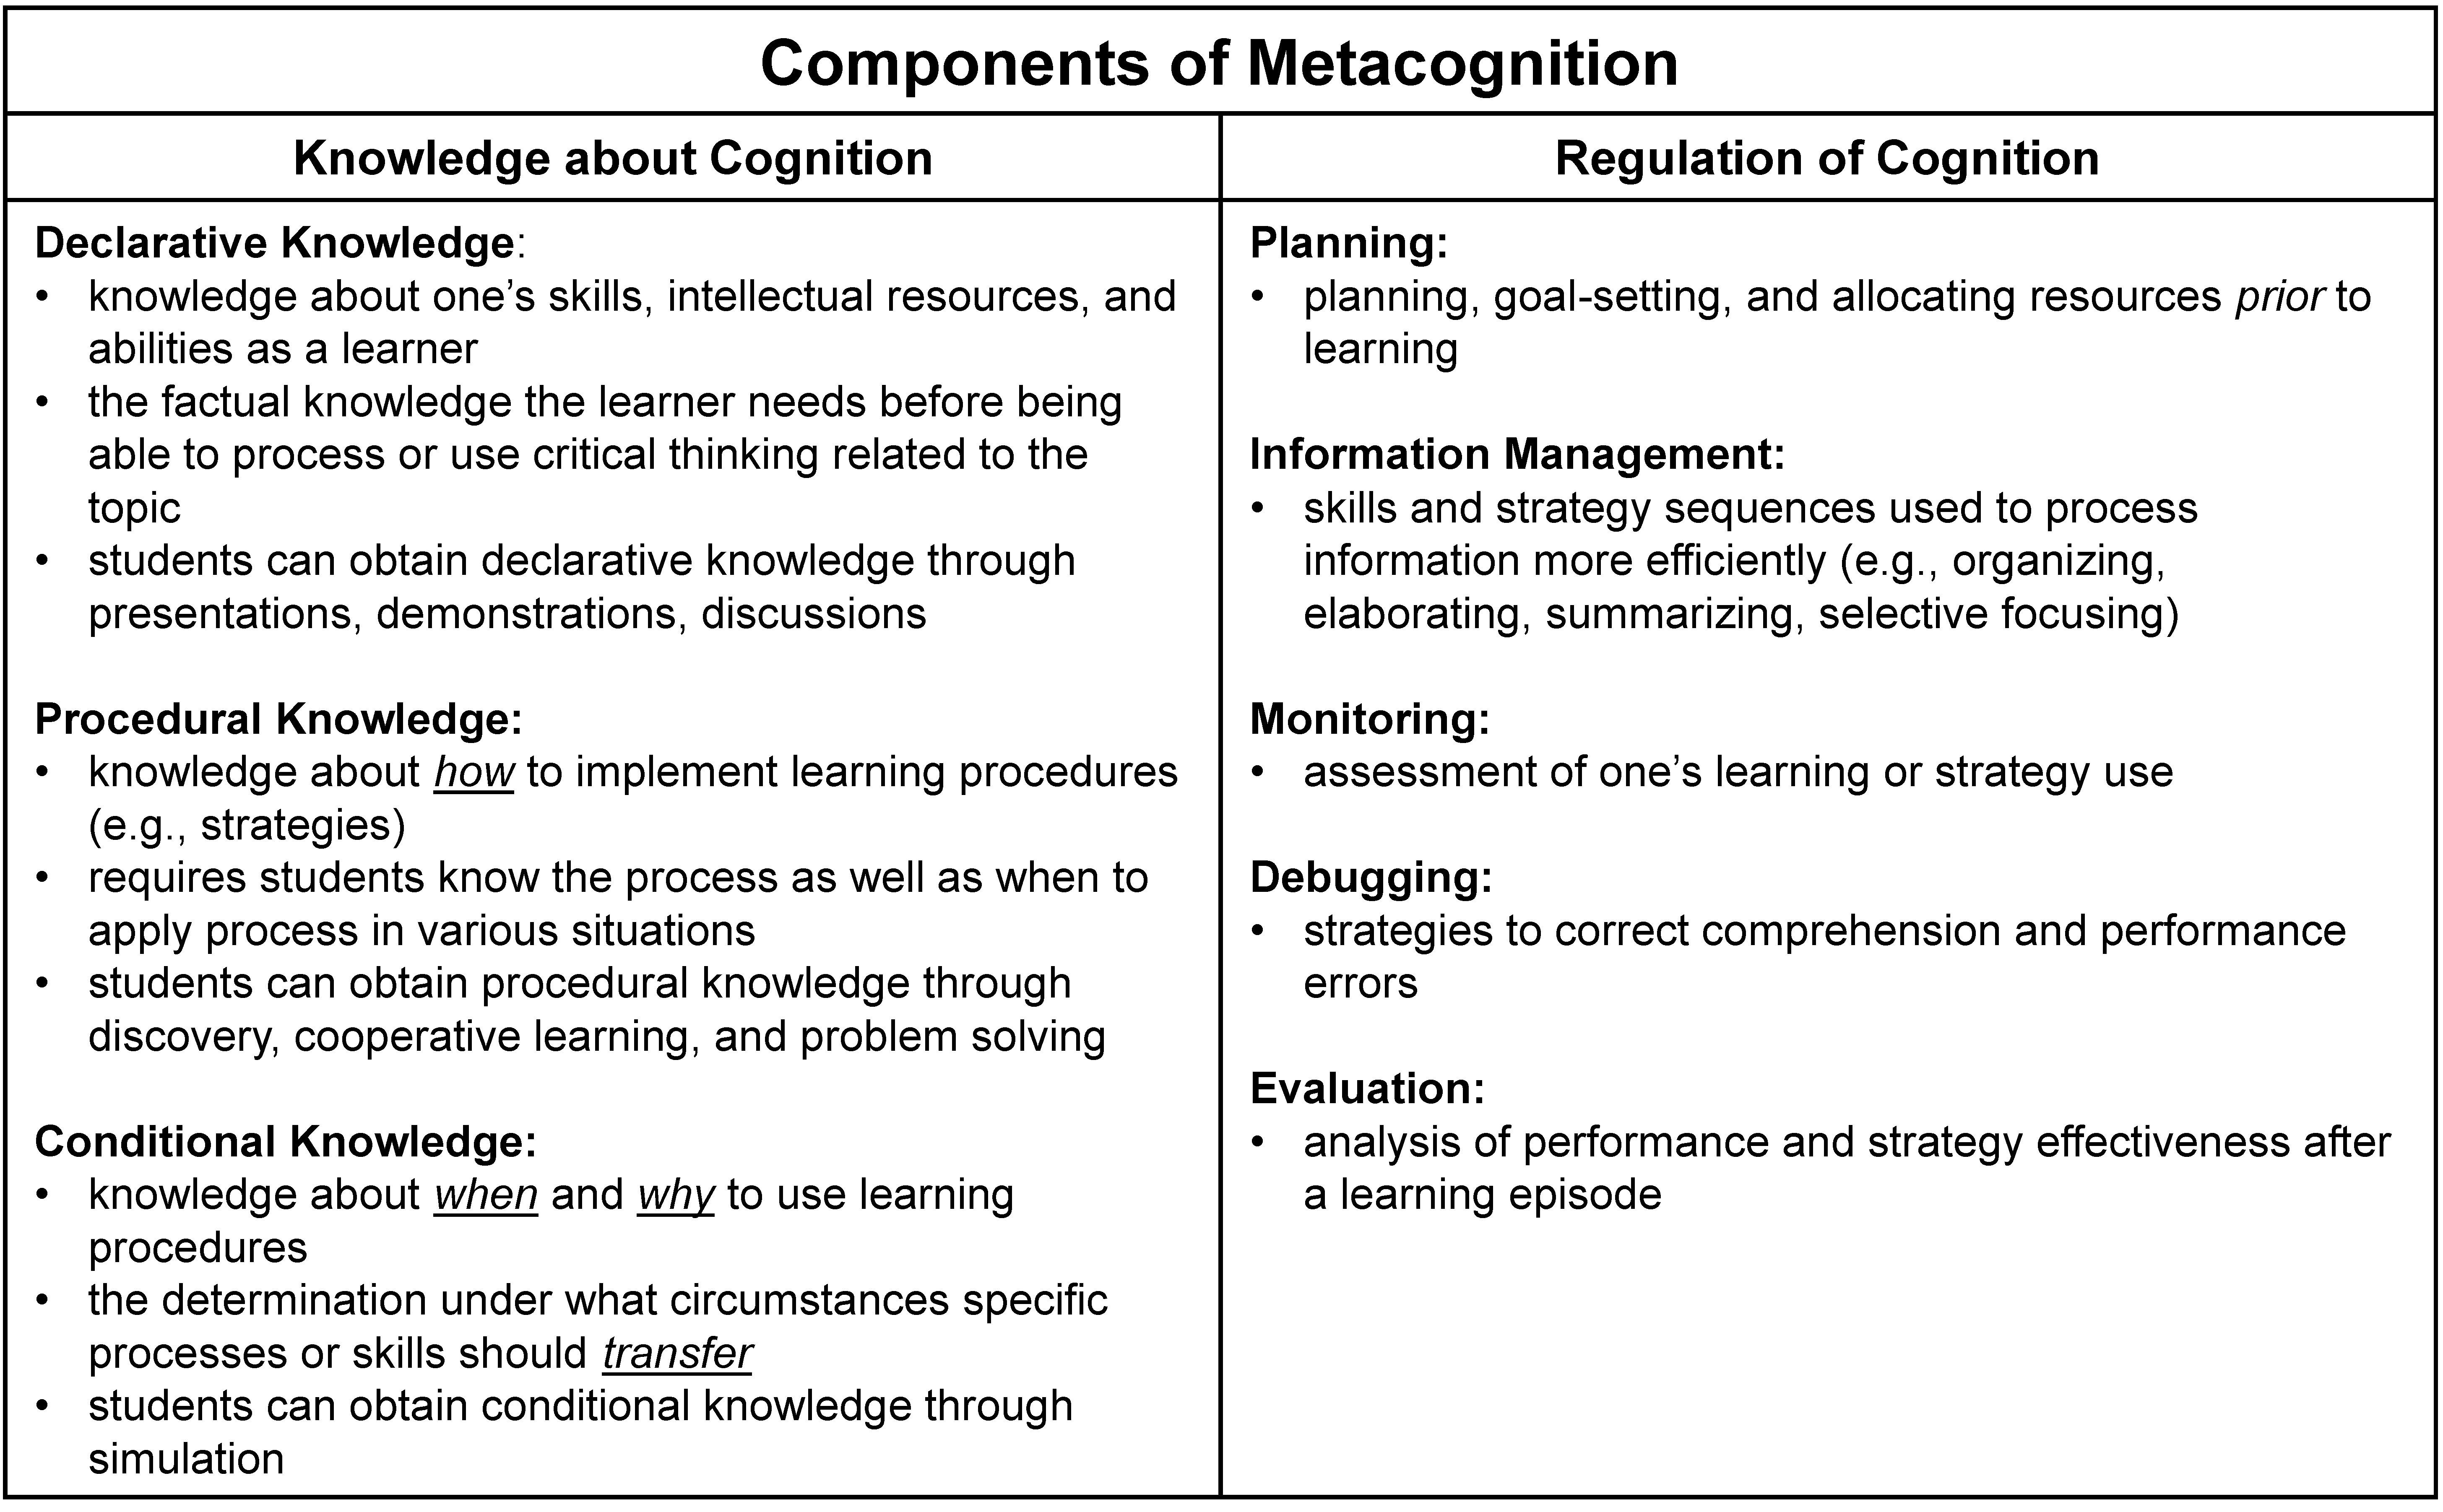
\includegraphics[width=1\linewidth]{figs/metacognition-components} 

}

\caption[Components of metacognition.]{Operational definitions and features of the metacognition components, adapted from Schraw \& Dennison (\protect\hyperlink{ref-schraw1994assessing}{1994}) and Vancouver Island University (\protect\hyperlink{ref-viu2021mai}{2021}).}\label{fig:metacognition-components}
\end{figure}





One of the reasons that articulation is so helpful to learning is that
it promotes \emph{reflection} or \emph{metacognition}. \textbf{Metacognition}, commonly
referred to as thinking about thinking, involves thinking at a higher
level of abstraction, which in turn improves thinking and learning
(\protect\hyperlink{ref-blanken2017metacognition}{Blanken-Webb, 2017}). It is ``the process of reflecting on and
directing one's own thinking'' (\protect\hyperlink{ref-council2000how}{National Research Council, 2000, p. 78}), and involves
thinking about the process of learning, and thinking about knowledge.
This ties forward to the self-regulation that effective learners exhibit
(Section \ref{sec-bg-learn-self-regulation}). Effective learners are aware
of their learning process, and can measure how efficiently they are
learning as they study.

The literature on metacognition broadly identifies two fundamental
components of metacognition: knowledge about cognition, and regulation
of cognition. \textbf{Knowledge about cognition} includes three subprocesses
that facilitate the \emph{reflective} aspect of metacognition: declarative
knowledge (knowledge about self and about strategies), procedural
knowledge (knowledge about how to use strategies), and conditional
knowledge (knowledge about when and why to use strategies). \textbf{Regulation
of cognition} include a number of subprocesses that facilitate the
\emph{control} aspect of learning. Five component skills of regulation have
been discussed extensively in the literature, including planning,
information management strategies, comprehension monitoring, debugging
strategies, and evaluation. The operational definitions of these
components are described in Figure \ref{fig:metacognition-components}

Schraw \& Dennison (\protect\hyperlink{ref-schraw1994assessing}{1994}) developed the \textbf{Metacognitive Awareness Inventory} (MAI) survey and a
scoring guide to measure these self-reported components and subprocesses
of metacognition. The original survey consists of 52 true/false
questions (Appendix \ref{app-qsnr-mai}), such as ``\emph{I consider several alternatives to a problem before I answer}'', ``\emph{I understand my intellectual strengths and weaknesses}'', ``\emph{I have control over how well I learn'', and ''I change strategies when I fail to understand}''.
The instrument has been widely used in research, and has its reliability and validity measures available. Later, Terlecki \& McMahon (\protect\hyperlink{ref-terlecki2018call}{2018}) proposed a revised version of the MAI, using five-point Likert-scales, ranging from ``\emph{I never do this}'' to ``\emph{I do this always}''.
They argue that when measuring change in metacognition over time, the Likert-scale based `how often' questions are more effective than dichotomous `Yes/No' questions (\protect\hyperlink{ref-terlecki2020revising}{Terlecki, 2020}; \protect\hyperlink{ref-terlecki2018call}{Terlecki \& McMahon, 2018}).

\hypertarget{motivation}{%
\subsection{Motivation}\label{motivation}}

\begin{figure}

{\centering 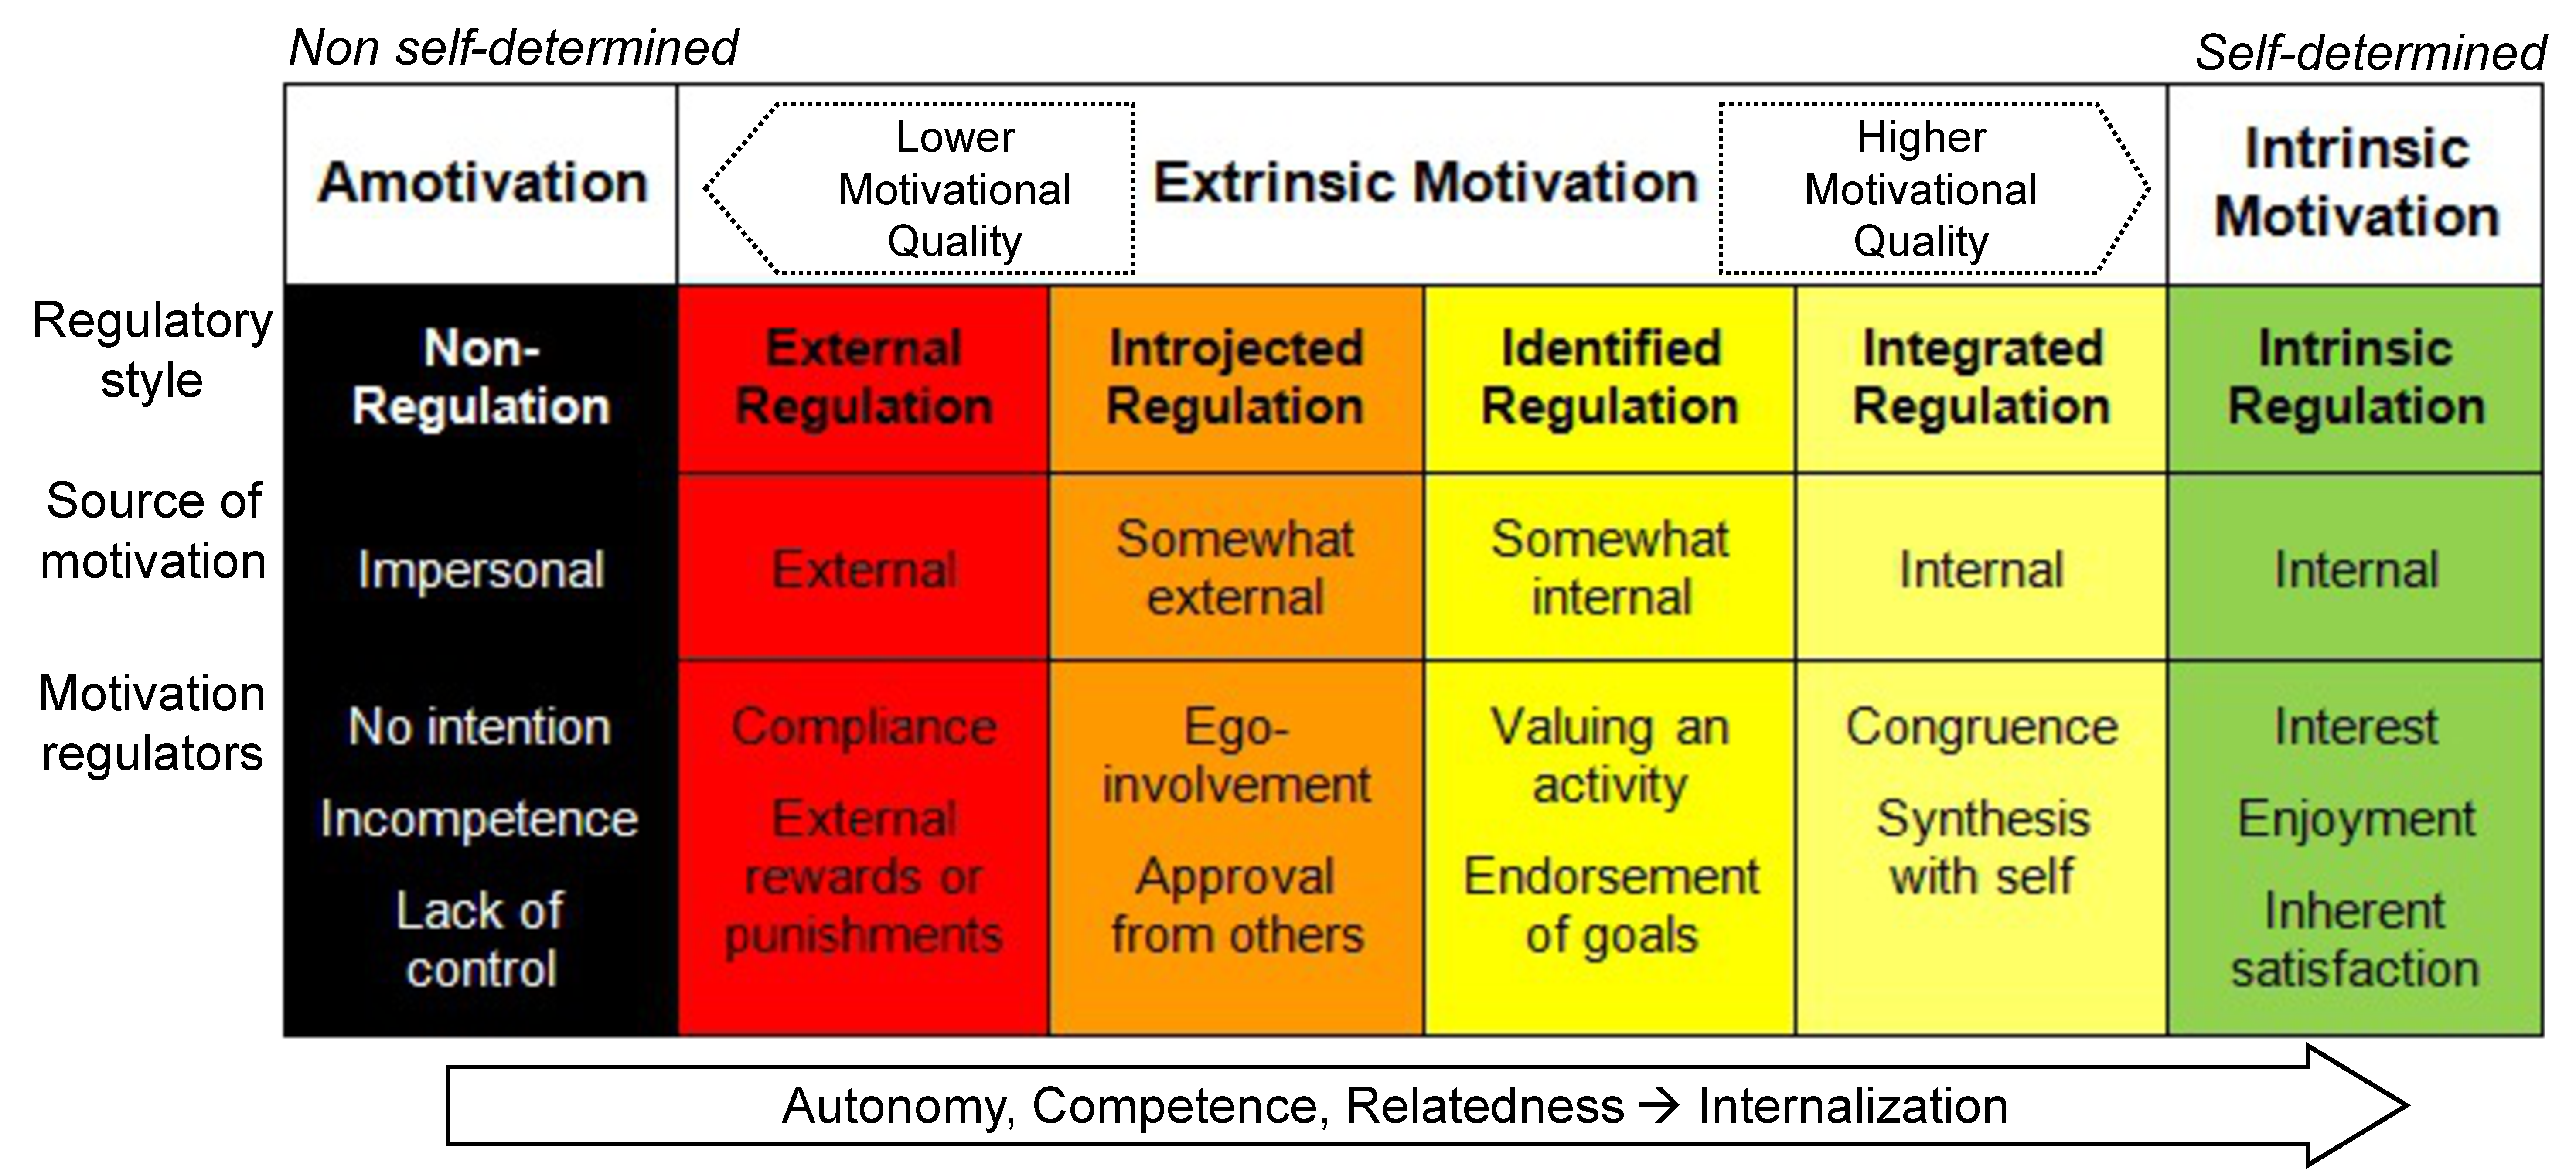
\includegraphics[width=1\linewidth]{figs/sdt-components} 

}

\caption[Motivation and self-determination continuum.]{The motivation and self-determination continuum, as proposed by the Self-Determination Theory (SDT). Figure adapted from Ryan \& Deci (\protect\hyperlink{ref-ryan2000intrinsic}{2000a}), Ryan \& Deci (\protect\hyperlink{ref-ryan2000self}{2000b}), and Guyan (\protect\hyperlink{ref-guyan2013improving}{2013}).}\label{fig:sdt-components}
\end{figure}





\textbf{Motivation} is the process that initiates, guides, and maintains
goal-oriented behaviours (\protect\hyperlink{ref-cherry2020what}{Cherry, 2020}). The \textbf{Self-Determination
Theory} (SDT) represents a broad framework for the study of human
motivation and personality (\protect\hyperlink{ref-ryan2017self}{Ryan \& Deci, 2017}). SDT differentiates the types
of motivation based on the reasons that give rise to behaviour:
intrinsic motivation and extrinsic motivation. \textbf{Intrinsic motivation}
is engaging in a task or behaviour for the rewards \emph{inside} the task or
behaviour, such the pleasure, enjoyment and satisfaction that the
behaviour provides. It is a stable form of motivation. \textbf{Extrinsic
motivation} is engaging in a task or behaviour for the rewards
\emph{outside} the task or behaviour, such as receiving rewards, avoidance of
punishment, gaining social approval, or achievement of a valued result.
Extrinsic motivation is on a continuum from less stable to more stable,
as illustrated in Figure \ref{fig:sdt-components}.
Extrinsic motivation does not last
unless the rewards and punishments are explicitly visible
(\protect\hyperlink{ref-deci2013intrinsic}{Deci \& Ryan, 2013}; \protect\hyperlink{ref-ryan2000self}{Ryan \& Deci, 2000b}; \protect\hyperlink{ref-tahamtan2019effect}{Tahamtan, 2019}).

Ryan (\protect\hyperlink{ref-ryan1982control}{1982}) proposed the \textbf{Intrinsic Motivation Inventory} (IMI)
(Appendix \ref{app-qsnr-imi}), a multidimensional questionnaire intended to
assess participants' subjective experience related to a target activity
in laboratory experiments. The instrument assesses participants'
interest/enjoyment, perceived competence, effort, value/usefulness, felt
pressure and tension, and perceived choice while performing a given
activity, yielding six subscale scores. The \emph{interest/enjoyment}
subscale is considered the most indicative self-report measure of
intrinsic motivation. The \emph{perceived choice} and \emph{perceived competence}
concepts are theorized to be positive predictors of both self-report and
behavioural measures of intrinsic motivation. The \emph{pressure/tension} is
theorized to be a negative predictor of intrinsic motivation. \emph{Effort}
is a separate variable that is relevant to some motivation questions, so
it is used if it is relevant. The \emph{value/usefulness} subscale is used to
measure internalization, with the idea being that people internalize and
become self-regulating with respect to activities that they experience
as useful or valuable for themselves.

\hypertarget{sec-bg-learn-self-regulation}{%
\subsection{Self-regulation}\label{sec-bg-learn-self-regulation}}

\textbf{Self-regulation} is the ability to develop, implement, and flexibly
maintain planned behaviour in order to achieve one's goals.
Self-regulation, and more broadly, self-direction, are critical to being
an effective ``lifelong'' learner. Self-regulation becomes increasingly
important at higher levels of education and in professional life, as
people take on more complex tasks and greater responsibilities for their
own learning. However, these metacognitive skills tend to fall outside
the content area of most courses, and therefore, often neglected in
instruction (\protect\hyperlink{ref-ambrose2010howa}{Ambrose et al., 2010, p. 191}). Building on the foundational work
of Kanfer (\protect\hyperlink{ref-kanfer1970self-a}{1970b}); Kanfer (\protect\hyperlink{ref-kanfer1970self-b}{1970a}), Miller and Brown formulated a
seven-step model of self-regulation (\protect\hyperlink{ref-brown1998self}{J. Brown, 1998}; \protect\hyperlink{ref-miller1991self}{W. R. Miller \& Brown, 1991}).
In this model, behavioural self-regulation may falter because of failure
or deficits at any of these seven steps: \emph{(i)} receiving relevant
information, \emph{(ii)} evaluating the information and comparing it to
norms, \emph{(iiii)} triggering change, \emph{(iv)} searching for options, \emph{(v)}
formulating a plan, \emph{(vi)} implementing the plan, and \emph{(vii)} assessing
the plan's effectiveness (which recycles to steps \emph{(i)} and \emph{(ii)}).
Although this model was developed specifically to study addictive
behaviours, the self-regulatory processes it describes are meant to be
general principles of behavioural self-control.
J. M. Brown et al. (\protect\hyperlink{ref-brown1999self}{1999}) developed the \textbf{Self-Regulation Questionnaire} (SRQ) (Appendix
\ref{app-qsnr-srq}) to
assess these self-regulatory processes through self-report. The items
were developed to mark each of the seven sub-processes of the
W. R. Miller \& Brown (\protect\hyperlink{ref-miller1991self}{1991}) model, forming seven subscales of the SRQ. The 63-item
scale elicits responses in the form of 5-point Likert scale, ranging
from strongly disagree to strongly agree. Based on clinical and college
samples, the authors tentatively recommend a score of 239 and above as
high (intact) self-regulation capacity (top quartile), 214-238 as
intermediate (moderate) self-regulation capacity (middle quartiles), and
213 and below as low (impaired) self-regulation capacity (bottom
quartile).

\hypertarget{self-directed-and-self-regulated-learning}{%
\subsubsection{Self-directed and Self-regulated Learning}\label{self-directed-and-self-regulated-learning}}

As we saw in the previous sections, self-regulation, motivation, and
metacognition are key concepts that moderate the learning process. These
terms are couched in the concepts of self-regulated learning and
self-directed learning.

\textbf{Self-directed learning} (SDL) is a ``process in which individuals take
the initiative, with or without the help from others, in diagnosing
their learning needs, formulating goals, identifying human and material
resources, choosing and implementing appropriate learning strategies,
and evaluating learning outcomes''(\protect\hyperlink{ref-knowles1975self}{Knowles, 1975, p. 18}).
\textbf{Self-regulated learning} (SRL) can be described as the degree to
which students are ``metacognitively, motivationally, and behaviourally
active participants in their own learning process'' (\protect\hyperlink{ref-zimmerman1989social}{Zimmerman, 1989, p. 329}).

\begin{figure}

{\centering 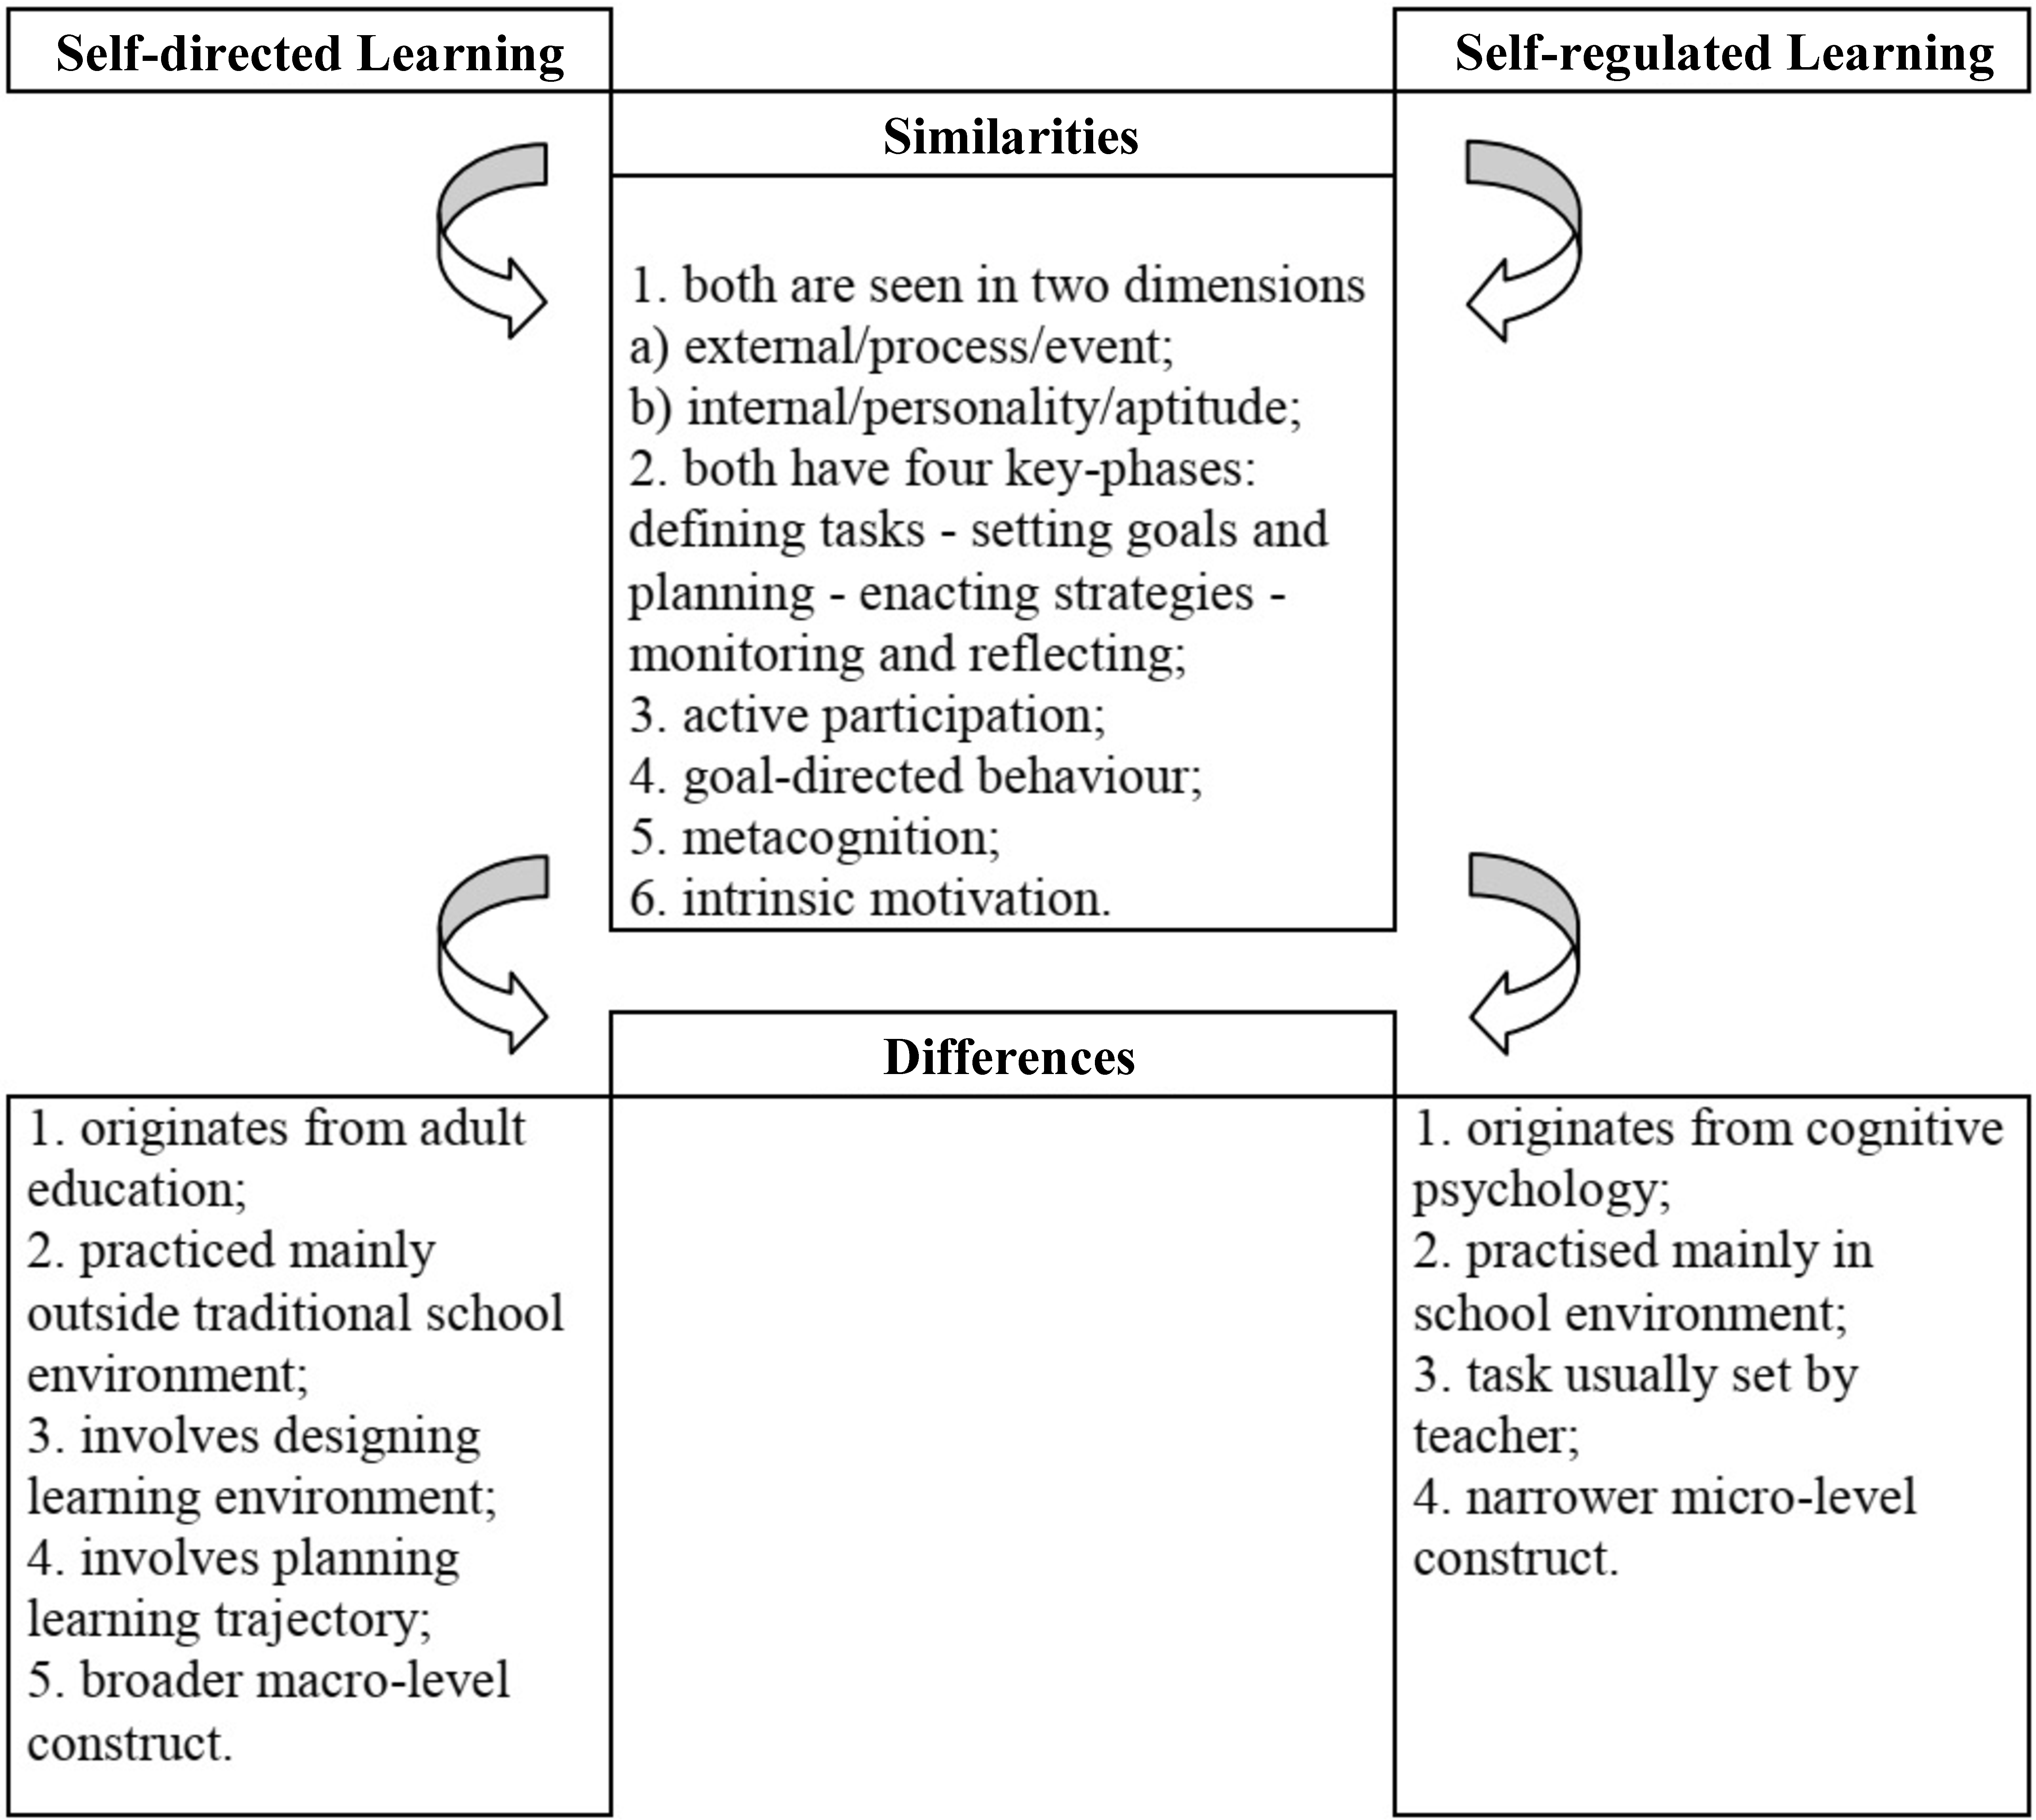
\includegraphics[width=0.8\linewidth]{figs/sdl-v-srl} 

}

\caption[Self-directed learning vs.~self-regulated learning.]{Self-directed learning vs.~self-regulated learning, as illustrated by Saks \& Leijen (\protect\hyperlink{ref-saks2014distinguishing}{2014}).}\label{fig:sdl-v-srl}
\end{figure}





Often used interchangeably, self-directed learning (SDL) and
self-regulated learning (SRL) have some important similarities and
differences (Figure \ref{fig:sdl-v-srl}) (\protect\hyperlink{ref-saks2014distinguishing}{Saks \& Leijen, 2014}). SDL, originating
from adult education, is a broader, macro-level construct, and is
usually practised outside the traditional school environment. The
self-directed learner is free to design their own learning environment,
and free to plan and set their own learning goals. SRL, on the other
hand, is a narrower, micro-level construct, originating from educational
and cognitive psychology, and is mostly utilized in the school
environment. Learners do not have as much freedom as in SDL. The
instructor or facilitator often defines the learning task and the
learning goals. Self-directed learning may include self-regulated
learning, but the converse is not true
(\protect\hyperlink{ref-jossberger2010challenge}{Jossberger et al., 2010}; \protect\hyperlink{ref-loyens2008selfdirected}{Loyens et al., 2008}). In other words, \emph{``a self-directed learner is supposed to self-regulate, but a self-regulated learner may not self-direct''} (\protect\hyperlink{ref-saks2014distinguishing}{Saks \& Leijen, 2014}). Despite their
differences, SDL and SRL share key similarities
(\protect\hyperlink{ref-saks2014distinguishing}{Saks \& Leijen, 2014}).
First, both can be seen in two dimensions:
\emph{(i)} \emph{external} to the learner, as a process or series of events, and
\emph{(ii)} \emph{internal} to the learner, arising from the learner's personality, aptitude, and individual differences.
Second, both the
learning processes have four key phases:
\emph{(i)} defining tasks,
\emph{(ii)} setting goals and planning,
\emph{(iii)} enacting strategies, and
\emph{(iv)} monitoring and reflecting.
Third, both SDL and SRL require active
participation, goal-directed behaviour, metacognition, and intrinsic
motivation.

In summary, metacognition is monitoring and controlling what is in the
learner's head; self-regulation is monitoring and controlling how the
learner interacts with their environment; self-regulated learning is the
application of metacognition and self-regulation to learning
(\protect\hyperlink{ref-mannion2020metacognition}{Mannion, 2020}); and the whole learning process is sustained
by motivation, which is desirable to be intrinsic.

\hypertarget{sec-bg-learn-summary}{%
\section{Summary and Implications for this Dissertation}\label{sec-bg-learn-summary}}

In this first chapter of the background literature review, we discussed
\emph{(i)} what is meaningful learning, a.k.a. deep learning, or sensemaking;
\emph{(ii)} how meaningful learning updates the learner's cognitive knowledge
structure; \emph{(iii)} how the learning process is influenced by digital
technologies, mass of information on the Internet, and IR systems; and
\emph{(iv)} what principles and practices learners and educators must realize
and follow to promote meaningful learning. These findings are from the
domains of Educational Sciences, Learning Sciences and Cognitive
Sciences. We argue that these are important aspects to be considered
when designing future IR or educational information systems that aim to
combine and improve the searching and learning experience.

Guided by these findings, we made some important decision choices for the longitudinal study conducted in this dissertation.
We aimed to situate learners in their context, and incorporate their individual differences using metacognition, motivation, and self-regulation characteristics.
Additionally, we aimed to assess learning using artefacts and concept maps.
We chose not use traditional tests like question-answers, and multiple choice assignments, since they are often not the preferred choice of knowledge-work output in real world scenarios.

In the next chapter, we look at relevant literature from the Information Sciences and Interactive Information Retrieval disciplines.

\hypertarget{ch-bg-search}{%
\chapter{Background: Information Searching}\label{ch-bg-search}}

This second chapter on background literature discusses relevant concepts
from the disciplines of Information Sciences, and more specifically
Interaction Information Retrieval. First, we introduce some terminology
around information behaviour, information need, and information
relevance. Then we discuss relevant findings various empirical studies,
from the lens of three-stage interactions in the information search
process. Then we discuss some overall generic characteristics of
information search behaviour, and how they are linked to expertise and
working memory. Next we discuss how learning has been assessed in recent
search-as-learning studies. We also discuss some limitations of current
search systems to foster learning, including the lack of sufficient
number of longitudinal studies. In the last section, we state what
implications these findings had for shaping the longitudinal study conducted for this
dissertation.

\hypertarget{sec-bg-search-terminology}{%
\section{Terminology}\label{sec-bg-search-terminology}}

\textbf{Information retrieval} (IR) is the process of obtaining \emph{information
objects}, that are \emph{relevant} to an \emph{information need}, from a
collection of those objects (Wikipedia). \textbf{Information objects} are
entities that can potentially convey information. They can take many
forms, such as documents, webpages, facts, music, spoken words, images,
videos, artefacts, and other forms of human expression. Areas where
information retrieval techniques are employed include search engines,
such as web search, social search, and desktop search; media search, as
in image, music, video; digital libraries and recommender systems, as
well as domain specific applications like geographical information
systems, e-Commerce websites, legal information search, and others.

Multiple perspectives exist around how users interact with information,
and IR systems. In the \textbf{Search Engine application view}, the
interactions are restricted to the search engine interface. In the
\textbf{Human-computer interaction} (HCI) view, interactions are between a
person and a system; but the system can go \emph{beyond} supporting only
retrieval, to supporting more complex tasks. In the \textbf{cognitive view of
IR}, which is the broadest, the interactions for obtaining information
can be between a person and a system, as well as between people, for
retrieval of information.

\begin{figure}

{\centering 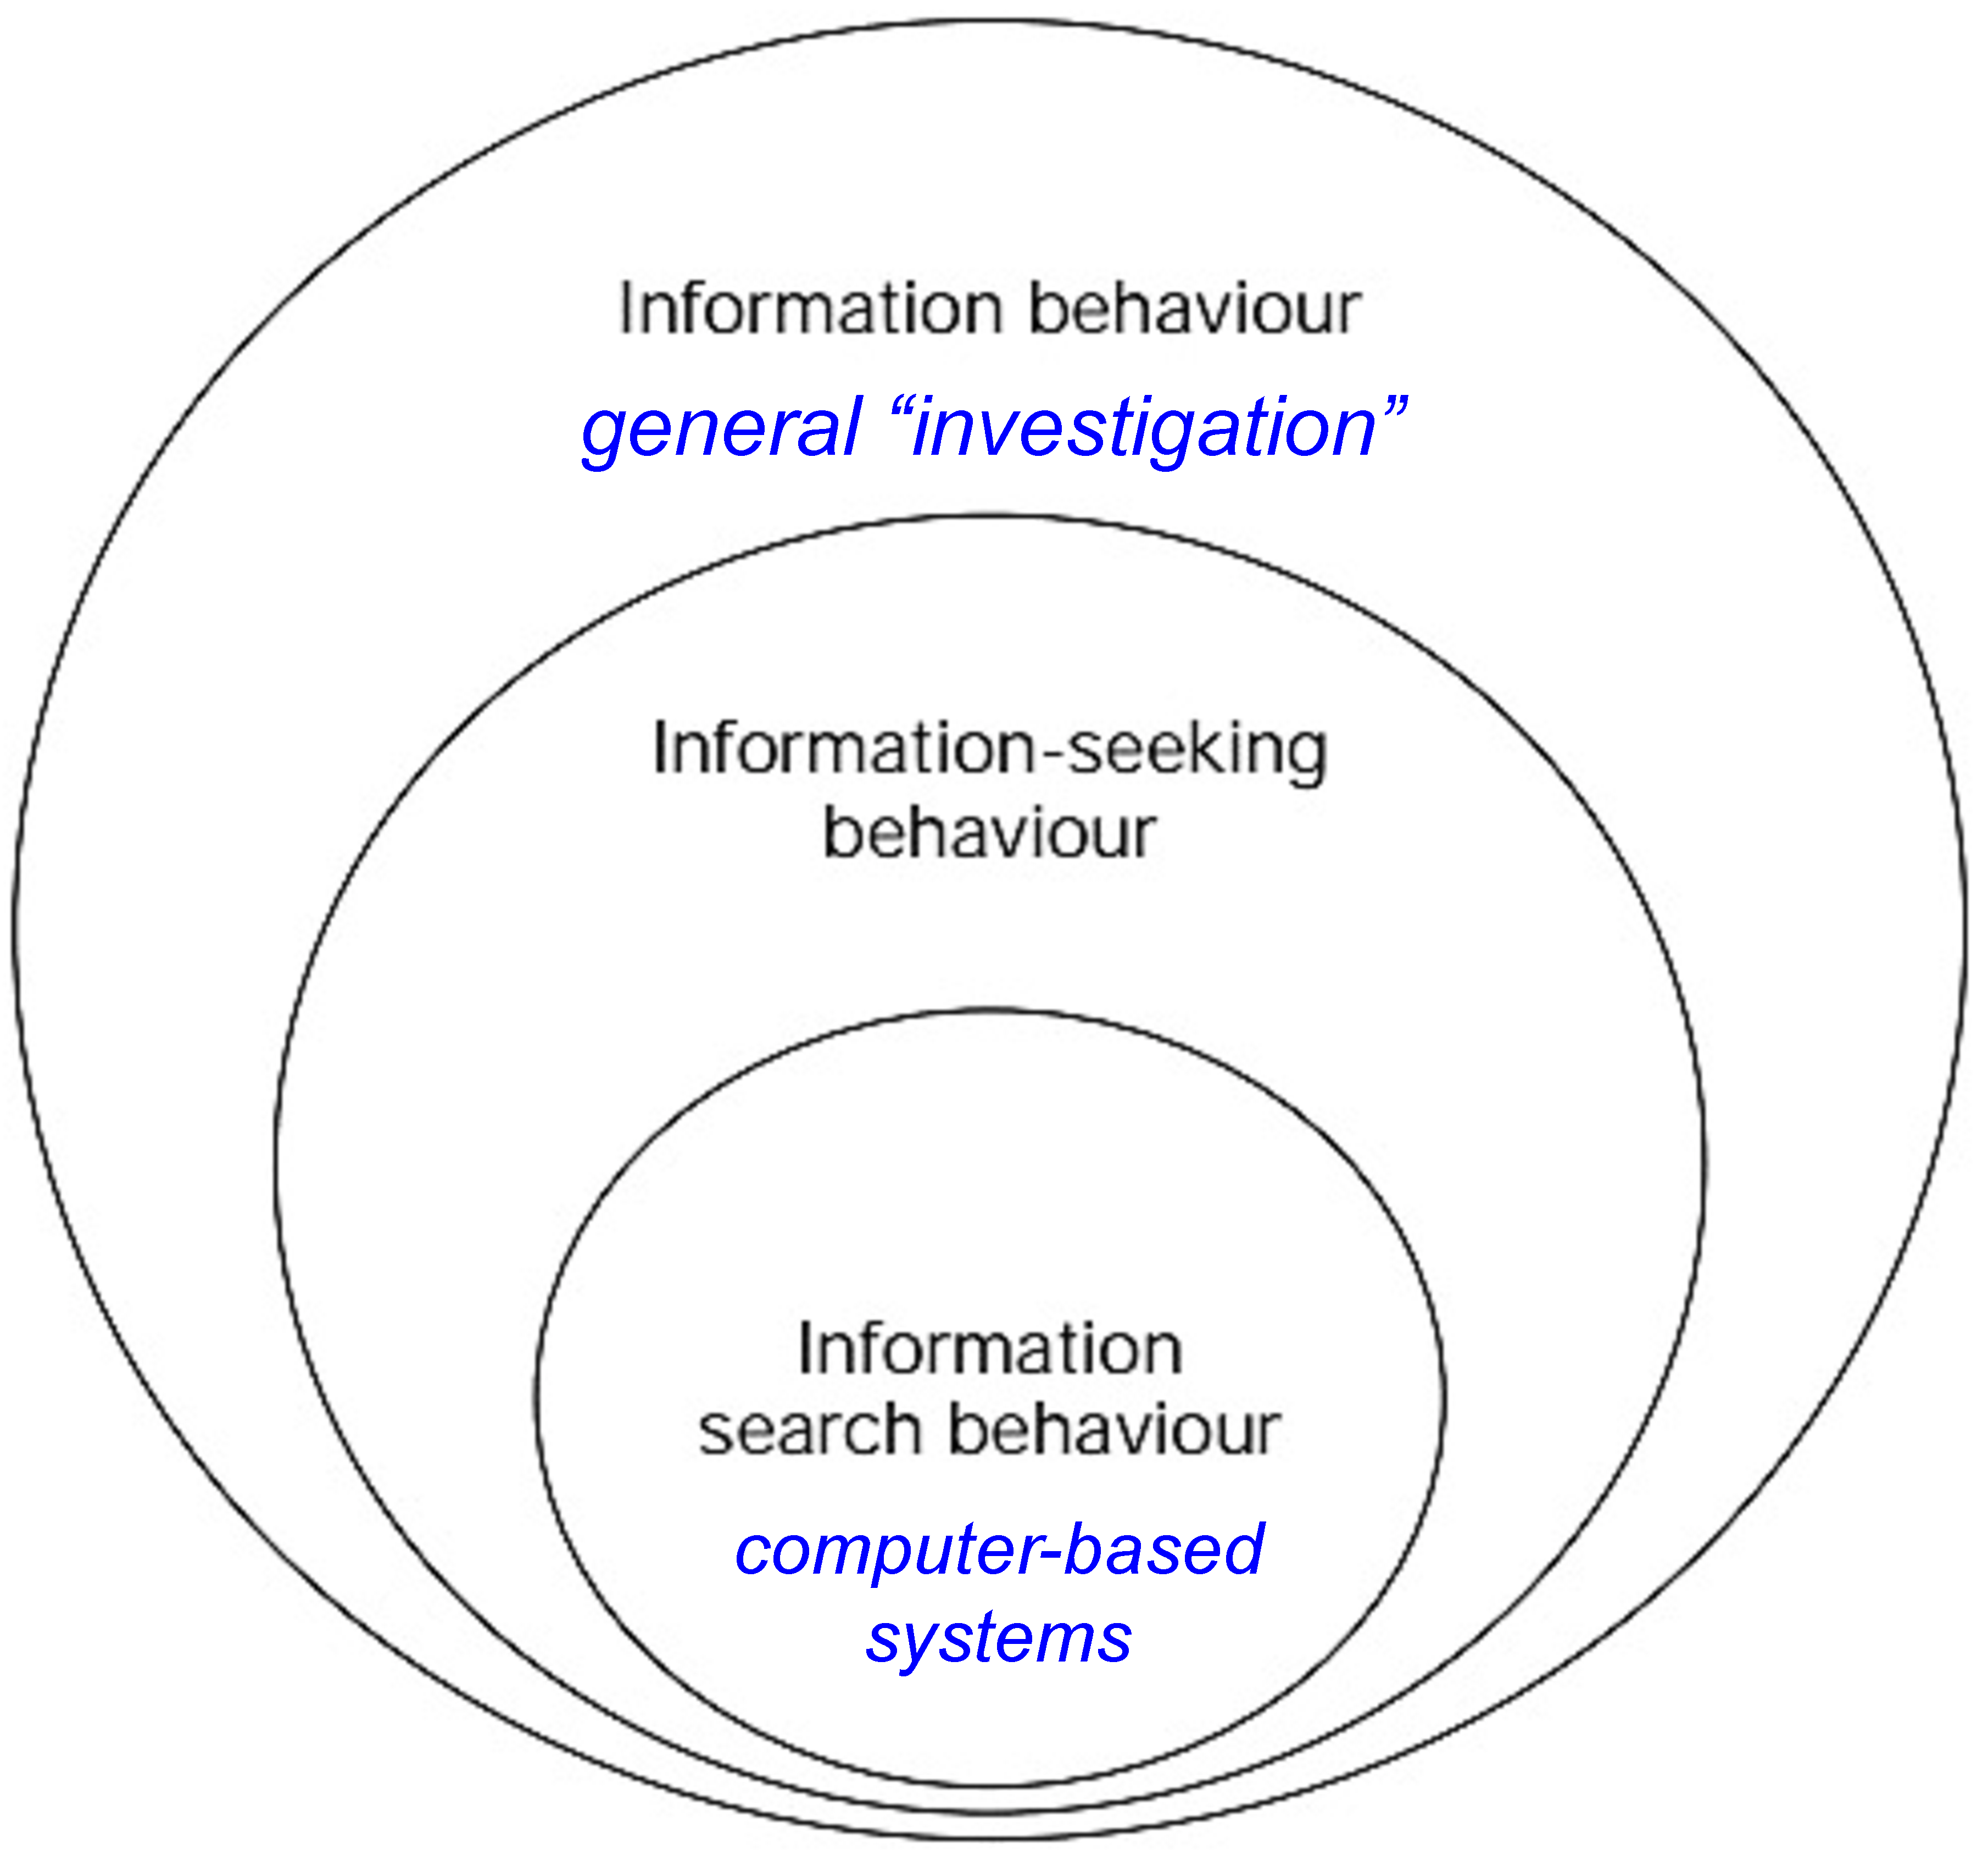
\includegraphics[width=0.5\linewidth]{figs/wilson-info-behaviour} 

}

\caption[Nested model of information behaviour by T. D. Wilson (\protect\hyperlink{ref-wilson1999models}{1999}).]{Nested model of information behaviour by T. D. Wilson (\protect\hyperlink{ref-wilson1999models}{1999}).}\label{fig:wilson-info-behaviour}
\end{figure}





People's behaviour around information can be modelled as a nested Venn
diagram as proposed by T. D. Wilson (\protect\hyperlink{ref-wilson1999models}{1999}) (Figure
\ref{fig:wilson-info-behaviour}). \textbf{Information behaviour} is
the more general field of investigation. \textbf{Information-seeking
behaviour} can be seen as a sub-set of the field, particularly
concerned with the variety of methods people employ to discover, and
gain access to information objects. \textbf{Information search behaviour} is
yet a sub-set of information-seeking, concerned with the interactions
between the user and computer-based information systems. In this
dissertation, we focus on information search rather than the other two
higher hierarchical concepts. This is because online IR systems, such as
search engines or digital libraries, have become the primary source for
people to obtain information in modern times, and web search is becoming
ever more pervasive and ubiquitous in our day-to-day lives.

The field of \textbf{interactive information retrieval} (IIR) posits that IR
systems should operate in the way that good libraries do. Good libraries
provide both the information a visitor needs, as well as a \emph{partner} in
the learning process --- the information professional --- to navigate
that information, make sense of it, preserve it, and turn it into
knowledge. As early as in 1980, Bertram Brookes stated that searchers
acquire new knowledge in the information seeking process
(\protect\hyperlink{ref-brookes1980foundations}{Brookes, 1980}). Fifteen years later, Gary Marchionini
described information seeking, as \emph{``a process, in which humans
purposefully engage in order to change their state of knowledge''}
(\protect\hyperlink{ref-marchionini1995information}{Marchionini, 1995}). So we have known for quite a while that
search is driven by the higher-level human need to gain knowledge.
Information Retrieval is thus a means to an end, and not the end in
itself. Thus, the ideal IR system should not only help users to locate
information, but also help them to \textbf{bridge the gap between information
and knowledge}.

This brings us to the concept of information need. \textbf{Information Need}
is the desire to locate and obtain information to satisfy a conscious or
unconscious human need. Most search systems of today assume that the
search query is an accurate representation of a user's information need.
However, Belkin et al. (\protect\hyperlink{ref-belkin1982ask}{1982}) observed that in many cases, users of search
systems are unable to precisely formulate what they need. They miss some
vital knowledge to formulate their queries. As humans, we have
difficulty in asking questions about what we do not know. Belkin called
this phenomenon as \textbf{Anomalous State of Knowledge}, or ASK. Later,
Huang \& Soergel (\protect\hyperlink{ref-huang2013relevance}{2013}) identified an exhaustive set of criteria that
should be considered in order to ideally represent a user's information
need. These criteria for information need are highly dependent on the
user context: user attributes, tasks or goals, as well as the situation
the user is embedded in. This brings us to another closely related
concept: information relevance.

\textbf{Relevance} is a fundamental concept of Information Science and
Information Retrieval, and perhaps the most celebrated work in this area
has been done by Tefko Saracevic
(\protect\hyperlink{ref-saracevic1975relevance}{Saracevic, 1975}, \protect\hyperlink{ref-saracevic2007relevance}{2007a}, \protect\hyperlink{ref-saracevic2007relevancea}{2007b}, \protect\hyperlink{ref-saracevic2016notion}{2016}).
Webster dictionary define relevance as ``a relation to the matter at
hand''. In most circumstances, relevance is a ``y'know'' notion. People
apply it effortlessly, without anybody having to define for them what
``relevance'' is. This creates one of the most fascinating challenges in
the information field: humans understand relevance intuitively, while it
is an open research problem to represent relevance effectively for use
by algorithmic systems. The situation becomes more interesting because
relevance always depends on context, and the context is ever dynamic, as
the matter at hand changes.

\hypertarget{sec-bg-search-3-stage}{%
\section{Three-stage Interactions with Online Search Systems}\label{sec-bg-search-3-stage}}

\begin{figure}

{\centering 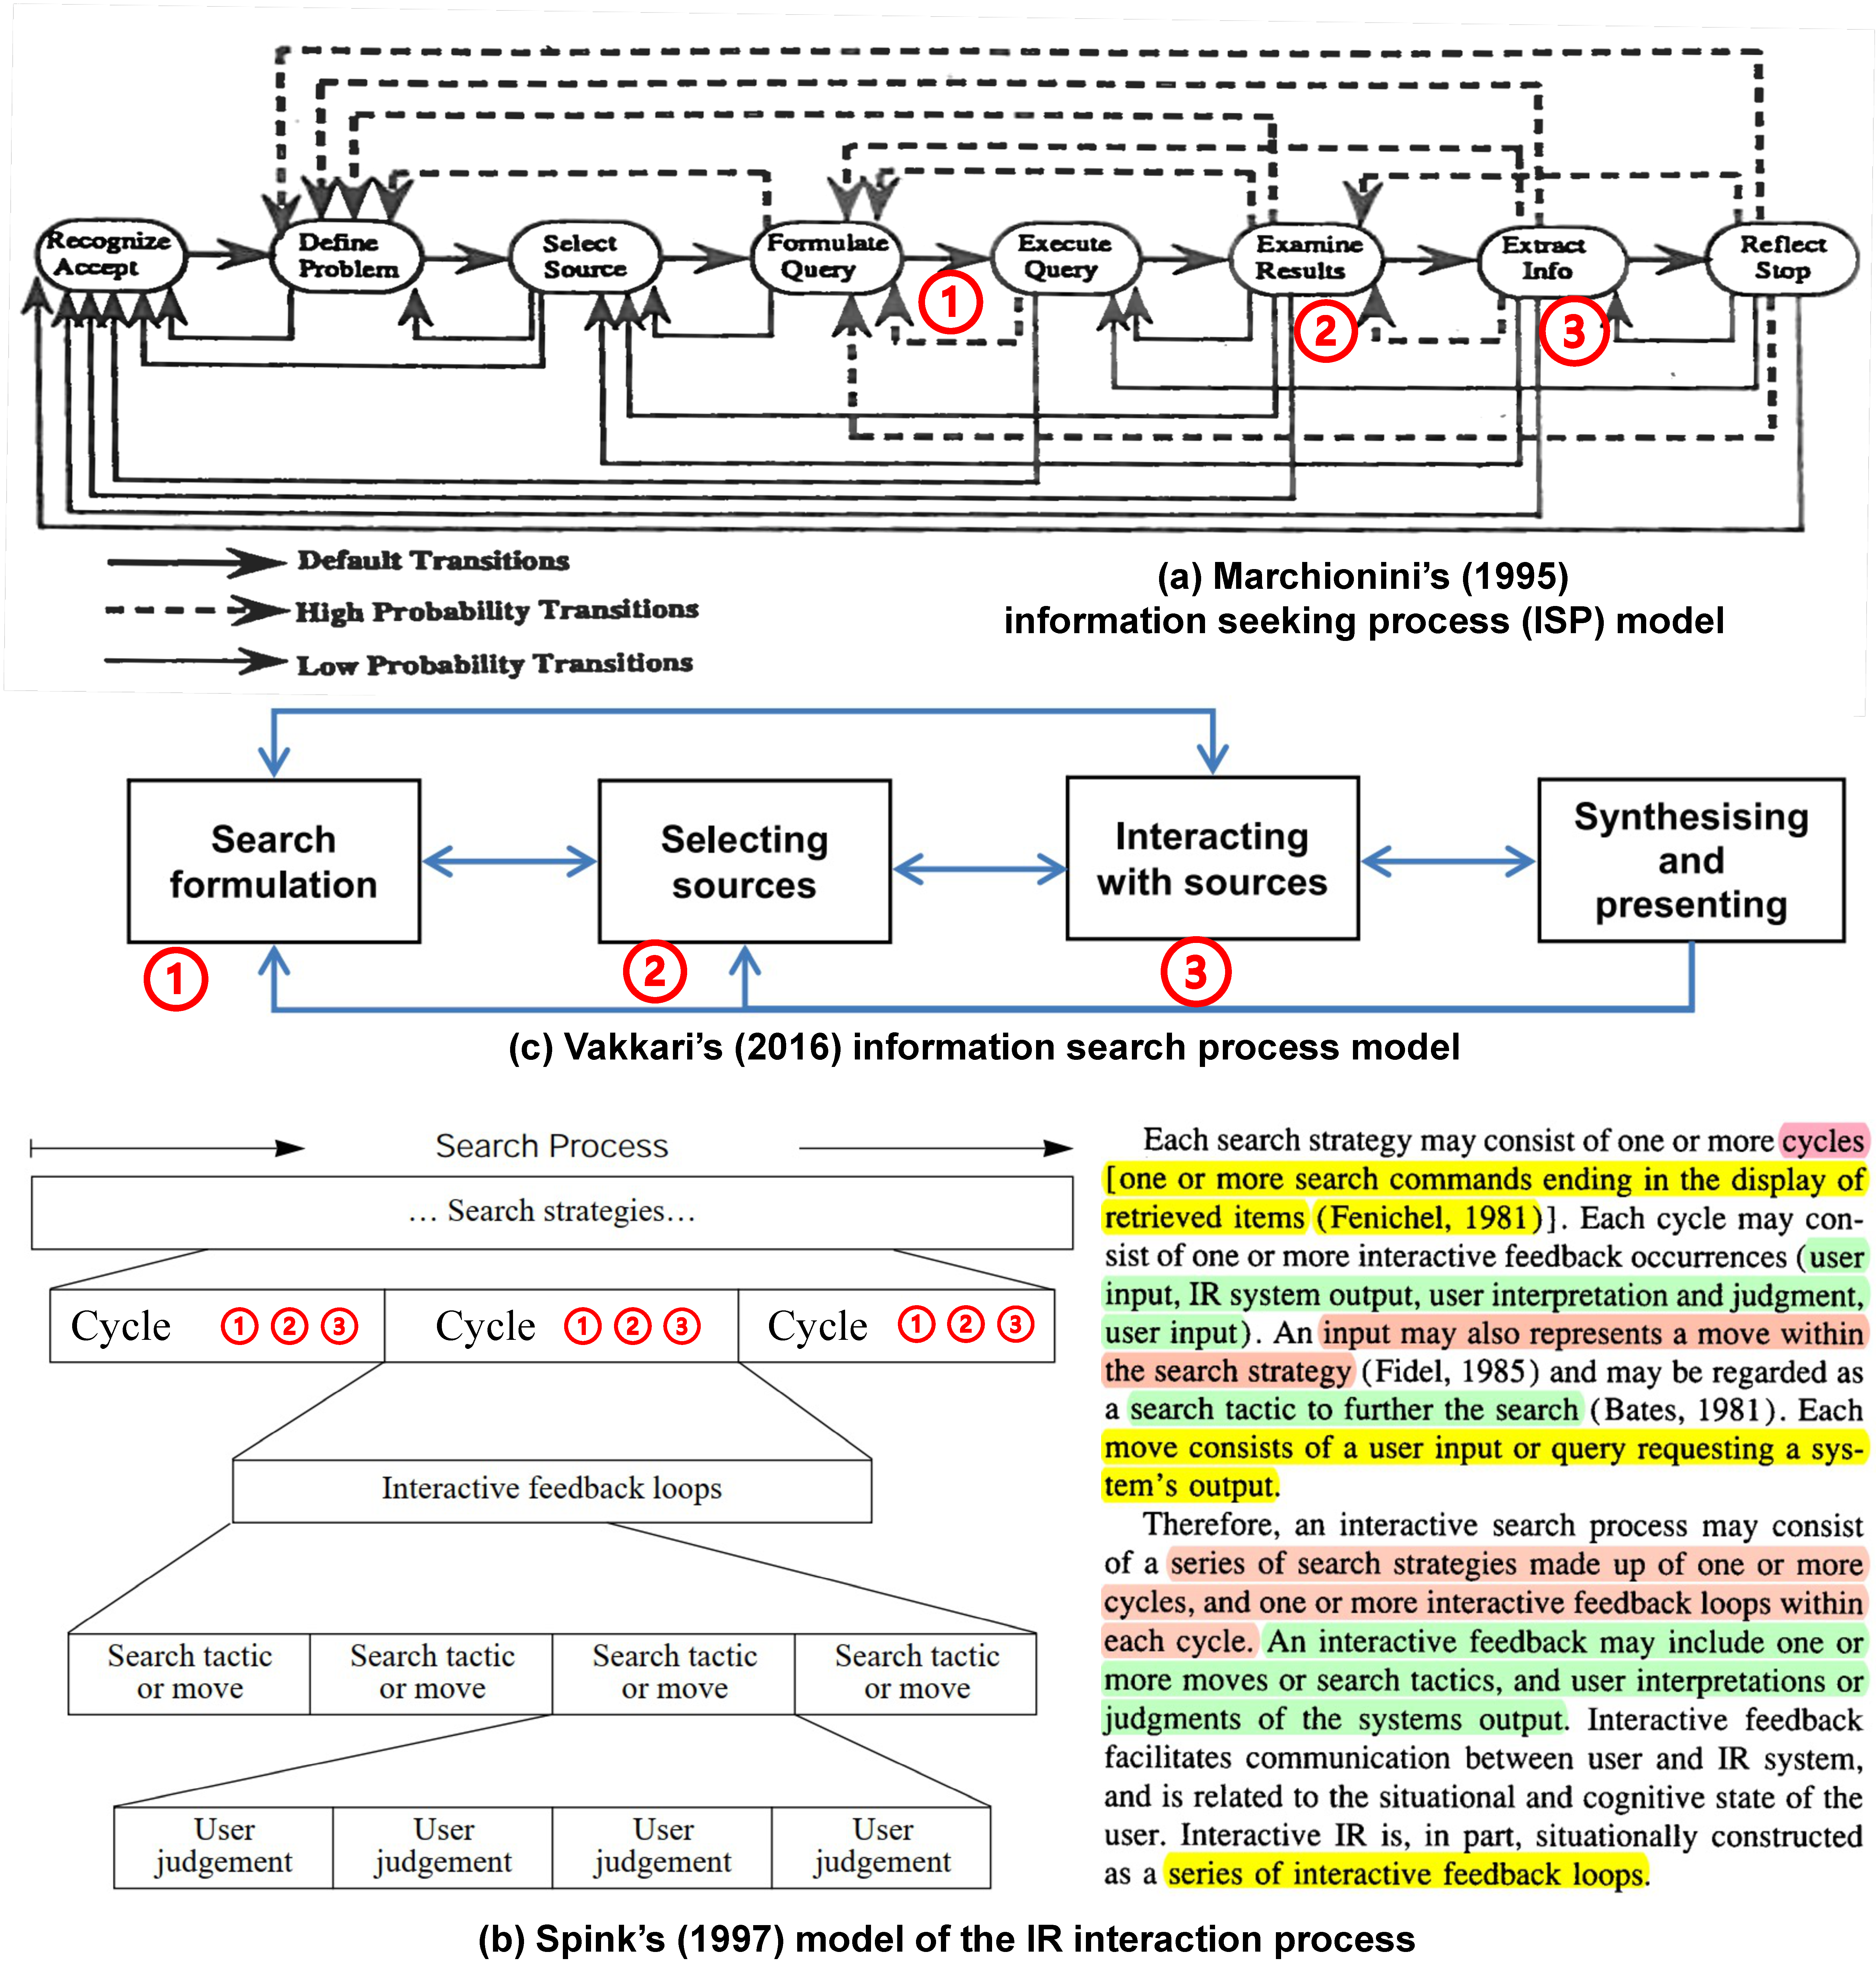
\includegraphics[width=1\linewidth]{figs/info-search-models} 

}

\caption[Models of information search process.]{Models of information search process, with our coloured annotations identifying the three stages: (1) query formulation, (2) list-item selection, and (3) item examination.}\label{fig:info-search-models}
\end{figure}





As we saw in the previous section, information search behaviour is the
(study of) interactions between a user, and digital Information
Retrieval (IR) systems. The field of Information Science/Studies has
developed multiple models explaining how information search works
(\protect\hyperlink{ref-wilson1999models}{T. D. Wilson, 1999}). A few of them are presented in Figure
\ref{fig:info-search-models}. Across many of these models, we
observe that most major Information Retrieval (IR) systems have three
fundamental ways of letting users interact with the system, and the
underlying information: \emph{(1)} an interface for entering search
\textbf{queries}; \emph{(2)} an interface for viewing and evaluating a \textbf{list} of
retrieved information-objects, or search results; \emph{(3)} an interface for
viewing and evaluating \textbf{individual information-objects}. For instance,
Marchionini (\protect\hyperlink{ref-marchionini1995information}{1995})'s ISP model hints at these three
interfaces in the fourth, sixth and seventh stages, namely ``formulate
query'', ``examine results'', and ``extract info''. Spink (\protect\hyperlink{ref-spink1997study}{1997})'s model
of the IR interaction process consists of sequential steps or cycles,
and each cycle comprises one or more interactive feedback occurrences of
user input (query), IR system output (list), and user interpretation and
judgement (of individual information-objects). Consequently, findings
from the large body of empirical research in interactive IR (especially
those with web based search systems) can be grouped around these thee
stages of interactions with search systems:

\begin{enumerate}
\def\labelenumi{\arabic{enumi}.}
\tightlist
\item
  \emph{Stage 1:} search query (re)formulation
\item
  \emph{Stage 2:} list-item selection: search results evaluation (aka source selection)
\item
  \emph{Stage 3:} item examination: content page evaluation (aka interacting with sources)
\end{enumerate}

The discussions in the following subsections are based around these
three stages of interactions. The empirical studies discussed below
generally follow some common principles of user studies in Interactive
IR (IIR) (\protect\hyperlink{ref-borlund2013interactive}{Borlund, 2013}; \protect\hyperlink{ref-kelly2009methods}{Kelly, 2009}): participants are
presented with a search task or search topic, and then they are asked to
search the internet (or a simulation of the open web) for information.
During the search, the various interactions (queries, clicks, webpages
opened etc.) are recorded, and these are analysed and correlated with
other sources of data to answer research questions.

\hypertarget{sec-bg-search-query}{%
\subsection{Stage 1: Query (Re)formulation}\label{sec-bg-search-query}}

\begin{quote}
\emph{How do users behave when submitting search queries (to an IR system)?}
\end{quote}

\begin{figure}

{\centering 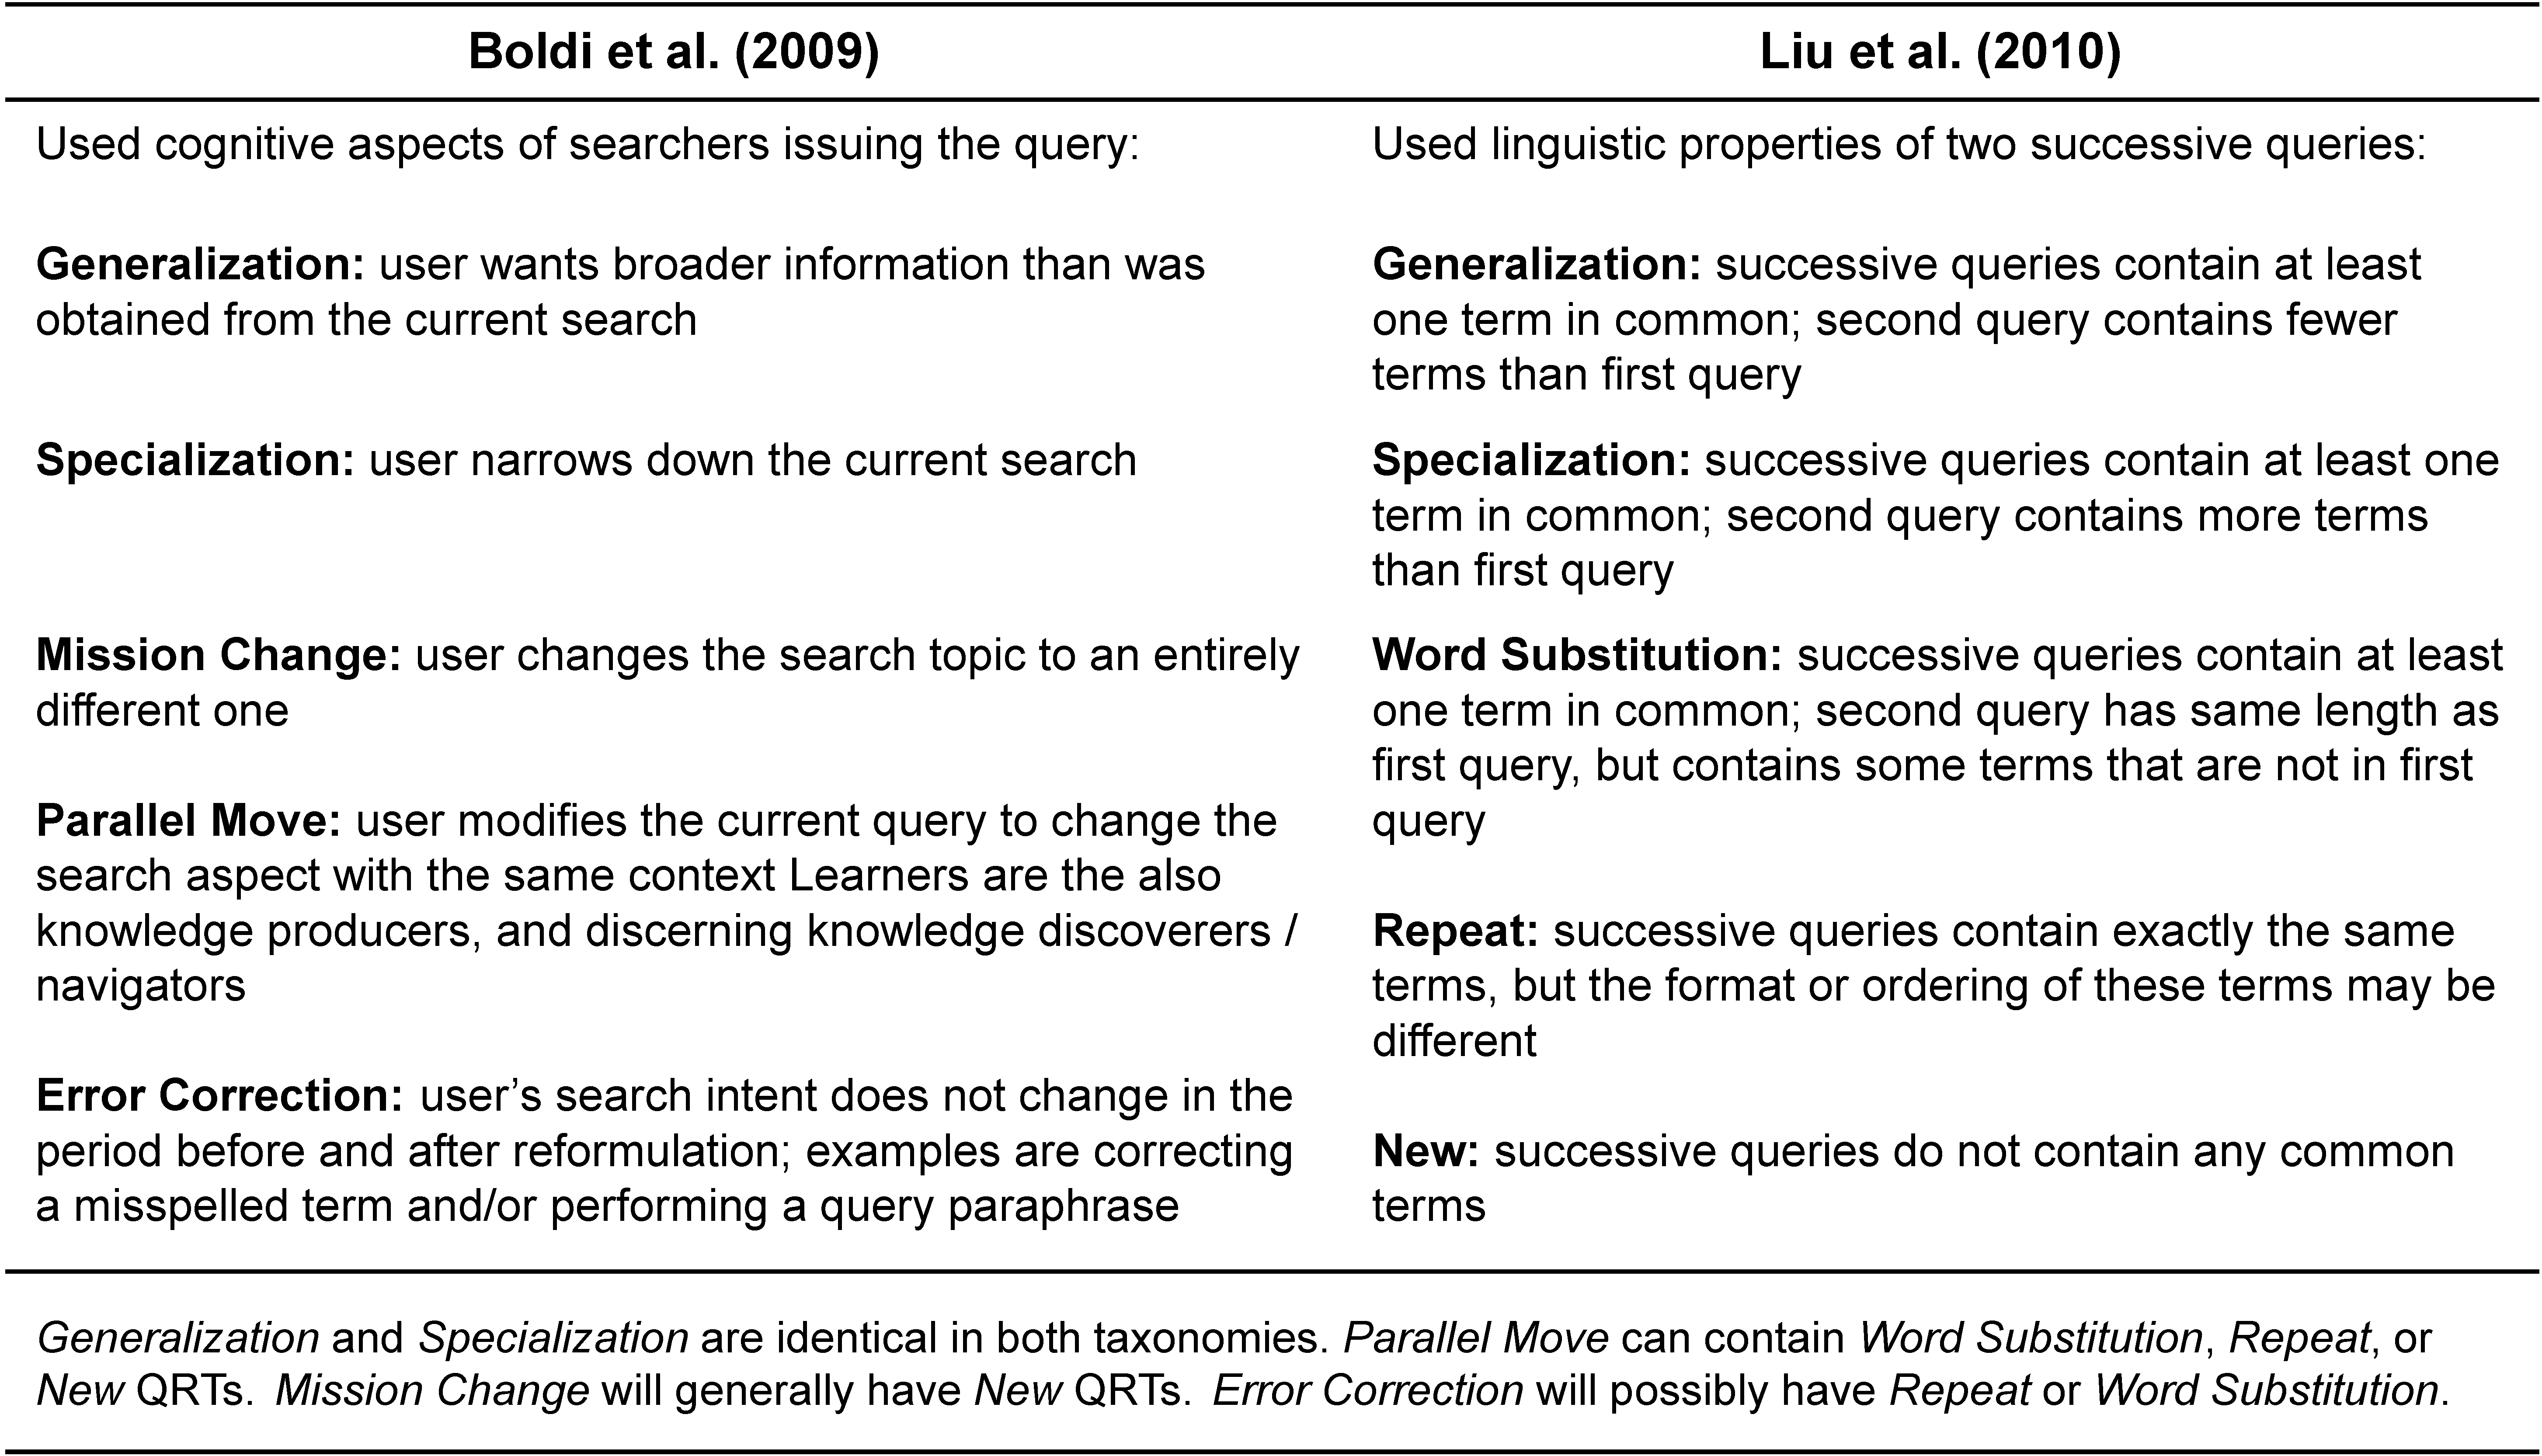
\includegraphics[width=1\linewidth]{figs/res-Q-QRT-txnmy} 

}

\caption[Comparison of Query Reformulation Types (QRTs) proposed in the literature.]{Comparison of Query Reformulation Types (QRTs) proposed by Boldi et al. (\protect\hyperlink{ref-boldi2009dango}{2009}) and C. Liu et al. (\protect\hyperlink{ref-liu2010analysis}{2010}).}\label{fig:res-Q-QRT-txnmy}
\end{figure}





\textbf{Query formulation} is the process of composing a search query that
describes the information need of a searcher. \textbf{Query reformulation}
refers to the act of either modifying a previous query, or creating a
new query. Query reformulation typically occurs due to a searcher's
improved understanding of how to better translate their information need
into a search query. The relationship between two successively issued
queries have been classified in a number of ways. These classifications
are called \emph{Query Reformulation Types}, or QRTs. Amongst many other,
Boldi et al. (\protect\hyperlink{ref-boldi2009dango}{2009}) used cognitive aspects of the searchers issuing the
query to propose a taxonomy of QRTs, while C. Liu et al. (\protect\hyperlink{ref-liu2010analysis}{2010}) proposed a
similar taxonomy focusing more on the linguistic properties of the two
successive queries. These are compared and contrasted in
Figure \ref{fig:res-Q-QRT-txnmy}.

Task-type, task-topic, task-goal, and domain-expertise were found to
influence query reformulation patterns of searchers (\protect\hyperlink{ref-127}{Eickhoff et al., 2015}; \protect\hyperlink{ref-126}{Jiang et al., 2014}; \protect\hyperlink{ref-133}{Mao et al., 2018}).
At first glance, a significant portion of the query reformulation terms
(\(\sim86\%\)) seemed to be coming from the task-description itself
(\protect\hyperlink{ref-126}{Jiang et al., 2014}; \protect\hyperlink{ref-133}{Mao et al., 2018}). This was characterized by significantly more fixations on
the task-description, rather than other SERP elements. Jiang et al. (\protect\hyperlink{ref-126}{2014}) and Mao et al. (\protect\hyperlink{ref-133}{2018})
investigated this phenomenon further. Jiang et al. (\protect\hyperlink{ref-126}{2014}) controlled for the task-type
and task-goal, using the faceted-framework by Li \& Belkin (\protect\hyperlink{ref-li2008faceted}{2008}). Mao et al. (\protect\hyperlink{ref-133}{2018})
controlled for the task-topic and the domain-expertise of the searchers.

If search tasks had \emph{factual} goals, searchers relied heavily on the
task-description for reformulating their queries (\protect\hyperlink{ref-126}{Jiang et al., 2014}). For
\emph{interpretive} tasks (intellectual tasks with specific goals), users
spent more time reading search result surrogates, before reformulating
their queries. This was observed by increased eye-fixations (indicative
of visual attention) and dwell time on search result snippets
(surrogates). For exploratory tasks, searchers fixated the longest on
query-autocompletion (QAC) suggestions, indicating that they were
possibly looking for help and suggestion based on their specific query,
as the search-task had non-specific (amorphous) goals.

Searchers also relied on the task-description for reformulating queries,
when the search-task was outside their domain of expertise (\protect\hyperlink{ref-133}{Mao et al., 2018}). For
in-domain tasks, they used query terms from their own knowledge, that
were not fixated on in visited SERPs and content pages. Eickhoff et al. (\protect\hyperlink{ref-127}{2015}) reported
that a significant share of new query terms came from visited SERPs and
content pages, and query reformulation (specialization) often did not
literally re-use previously encountered terms, but highly related
ones \footnote{
  measured using Leacock-Chodorow semantic similarity metric (\protect\hyperlink{ref-leacock1998combining}{Leacock \& Chodorow, 1998})} instead. These observations can possibly be explained by Mao et al. (\protect\hyperlink{ref-133}{2018})'s
findings: when exploring a new domain, the searcher may accumulate
vocabulary and learn how to query during the search; when performing
in-domain search-tasks, the searcher may have enough prior knowledge to
come up with effective query terms. It was also seen that searchers from
medicine domain used more unread query terms for their in-domain
search-tasks, compared to politics and environment domains (\protect\hyperlink{ref-133}{Mao et al., 2018}). This
suggested that domain knowledge and expertise is more important for
formulating good search queries in highly technical disciplines (e.g.,
medicine), compared to less technical domains (e.g., politics).

\begin{figure}

{\centering 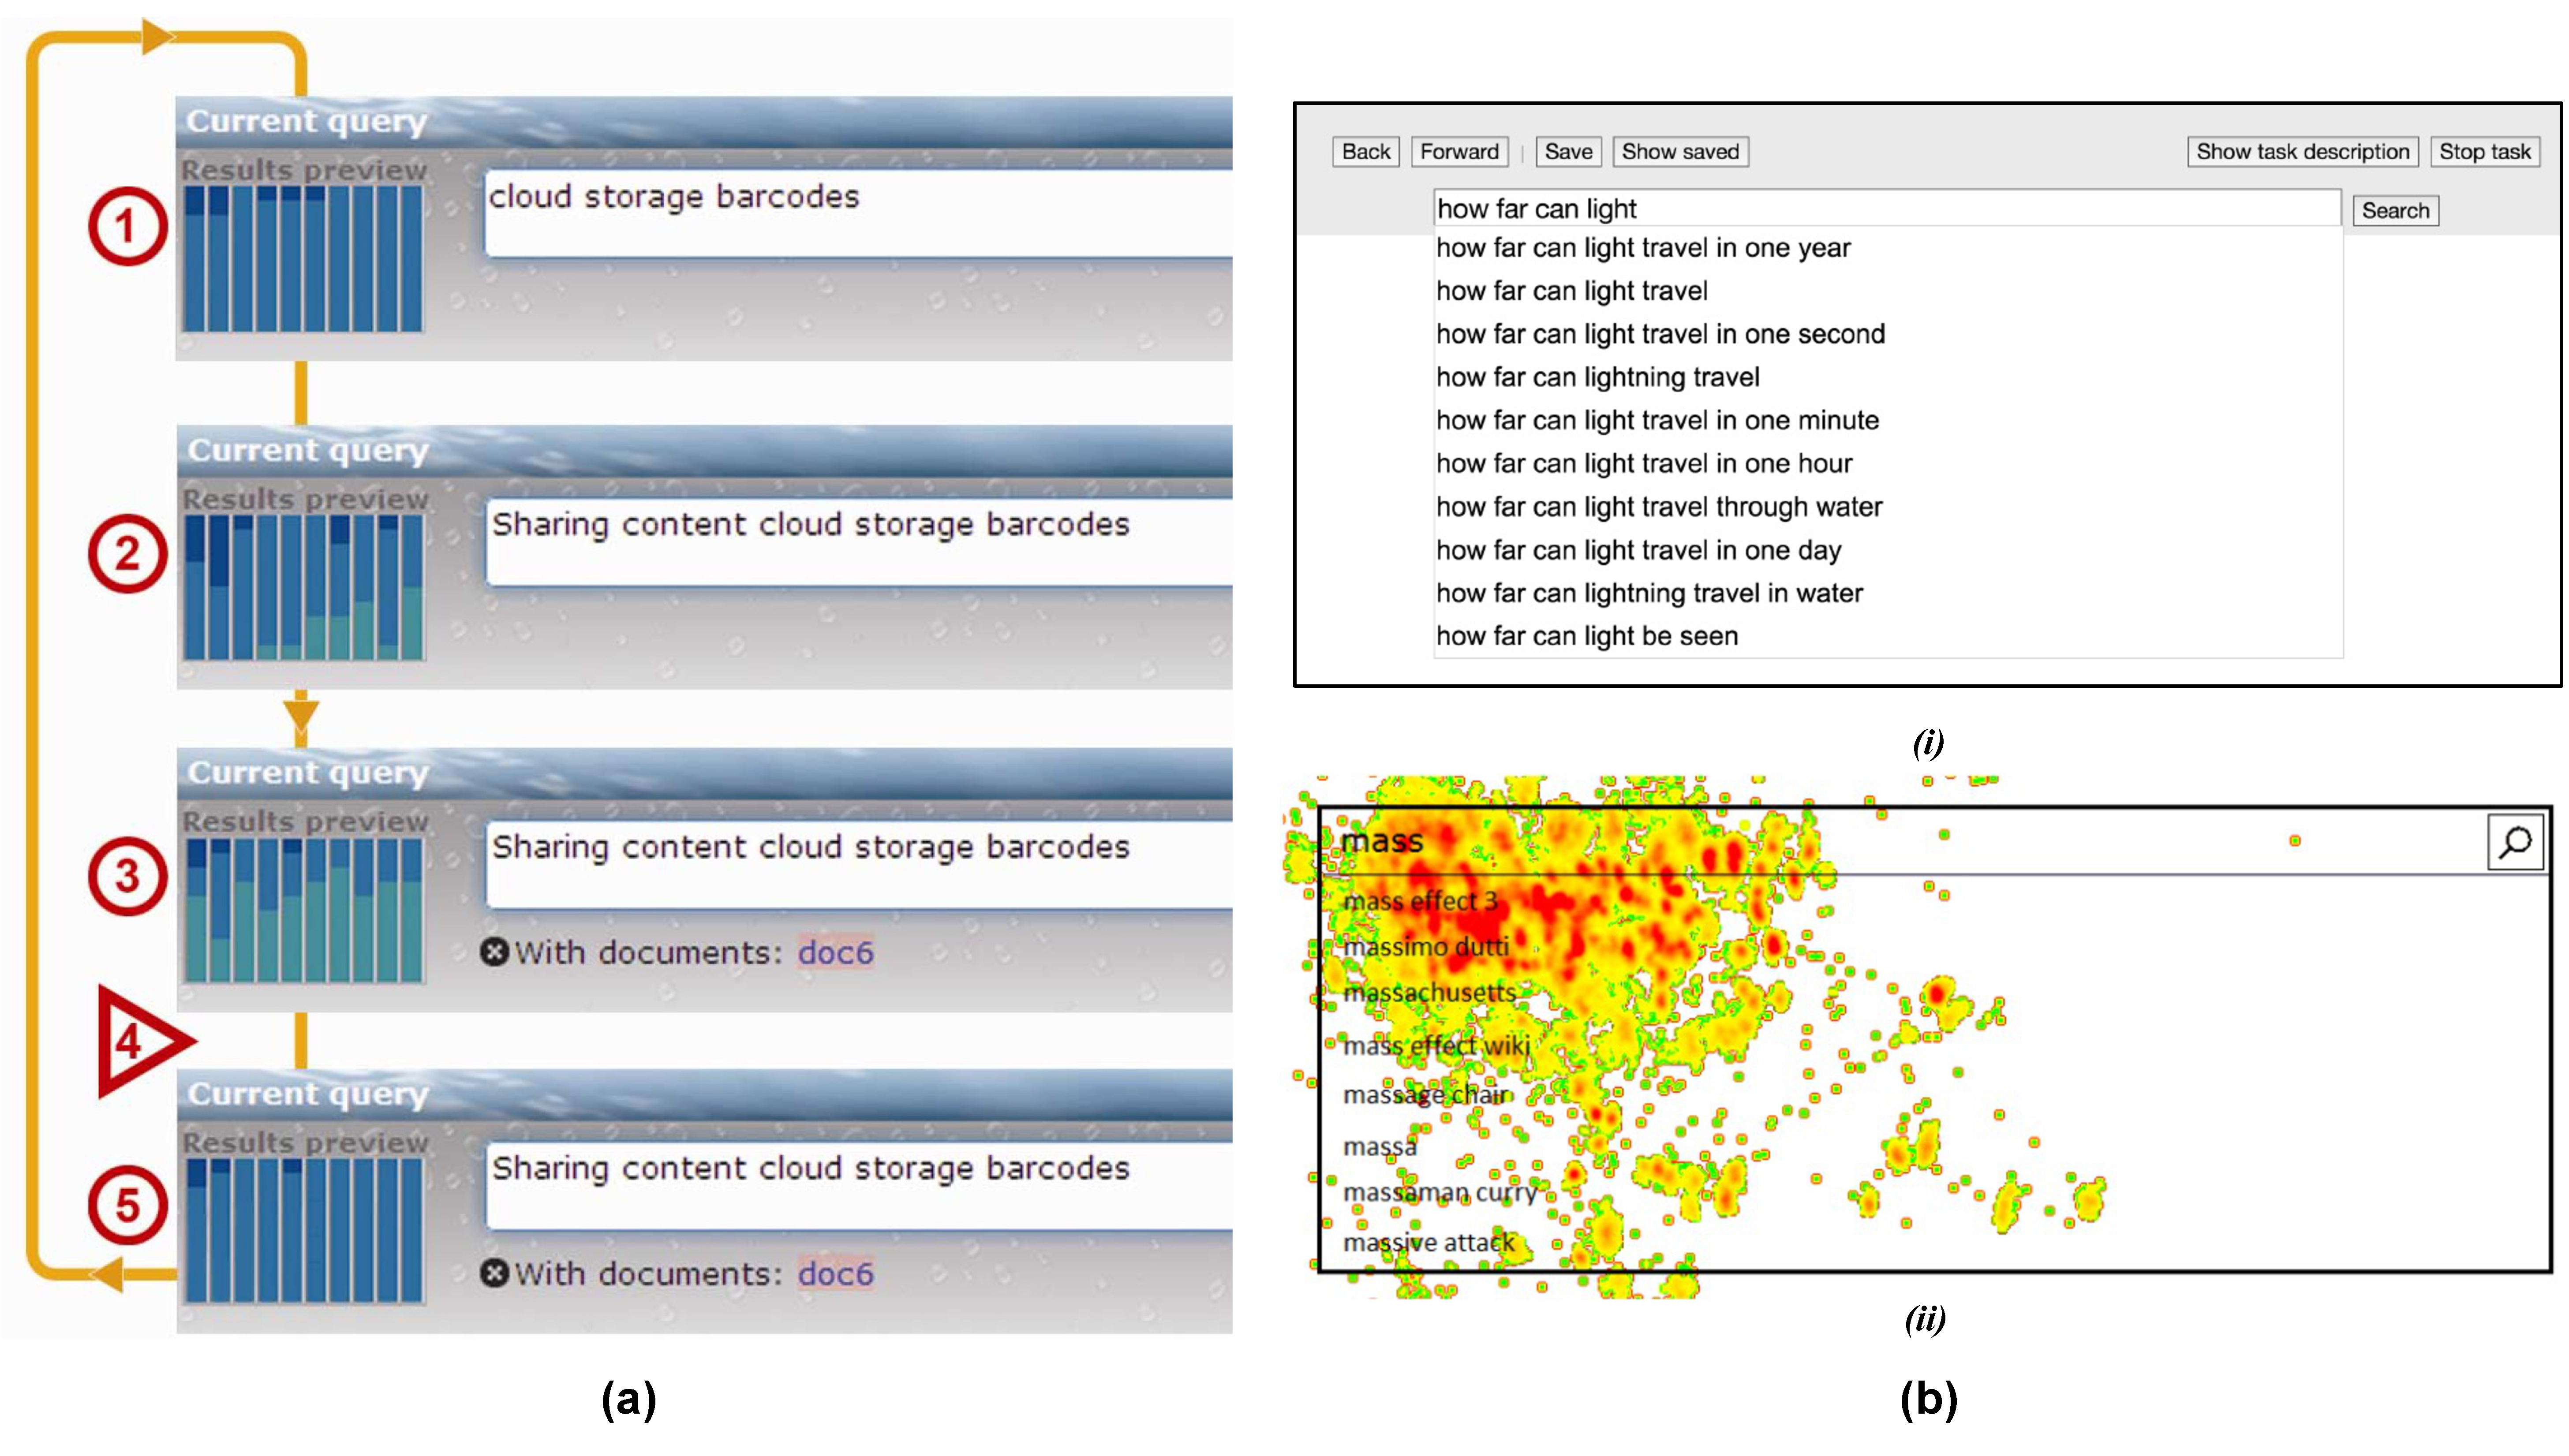
\includegraphics[width=1\linewidth]{figs/int-Q} 

}

\caption[Investigating user-interactions with queries.]{Investigating user-interactions with queries: \textbf{(a)} Visualizing the distribution of retrieved search results prior to running a query, for helping searchers understand their queries' effectiveness (\protect\hyperlink{ref-121}{Qvarfordt et al., 2013}). The visualization is a stacked column chart with ten columns. Each column represents ten search results: first column represents results ranked 1-10, second column represents results 11-20, etc. Individual columns have three divisions, indicating the counts of results that: are already seen by the searcher (dark blue, top), will be re-retrieved, but have not been seen by the searcher (medium blue, middle), and will be newly-retrieved (bright teal blue, bottom). The system evaluates the searcher's query continuously as it is being typed, and updates the visualization in real-time. \textbf{(b)} Interfaces for examining interactions with query auto-completion (QAC), by \textbf{\emph{(i)}} Smith et al. (\protect\hyperlink{ref-129}{2016}), and \textbf{\emph{(ii)}} Hofmann et al. (\protect\hyperlink{ref-125}{2014}) (overlaid with heatmaps of eye fixations for all participants). This figure is best viewed in colour.}\label{fig:int-Q}
\end{figure}





\textbf{Query Auto Completion (QAC)} is a technological feature that suggests
possible queries to web search users from the moment they start typing a
query. It is nearly ubiquitous in modern search systems, and is thought
to reduce physical and cognitive effort when formulating a query. QAC
suggestions are usually displayed as a list
(Figure~\ref{fig:int-Q}(b)
and (c)), and users interact in a variety of ways with the list. Hofmann et al. (\protect\hyperlink{ref-125}{2014})
observed a strong position bias among searchers who examined the QAC
list: the top suggestions received the highest visual attention, even
when the ordering of the suggestions were randomized. Average fixation
time decreased consistently on suggested items from top to bottom. Even
when the ranking of suggestions were randomized, time taken to formulate
queries did not significantly differ.

Search topics were found to have a large effect on QAC usage
(\protect\hyperlink{ref-126}{Jiang et al., 2014}; \protect\hyperlink{ref-129}{Smith et al., 2016}). Search was easiest for the topics with the highest QAC
usage. Total eye-gaze duration was longest when visual attention was
shared between the QAC suggestions and the actual search query input
box. Some additional time was probably due to decision making on whether
to use a QAC suggestion. Typing was faster when a QAC was not used.
However, the IR system's retrieval performance (measured using NDCG@3),
was greater when QAC was used. So Smith et al. (\protect\hyperlink{ref-129}{2016}) speculated that the value of
using QAC suggestions was realized later in the search session by users,
when they saw a reduction in the number of additional queries needed, or
an increase in the value of the information found.

\begin{figure}

{\centering 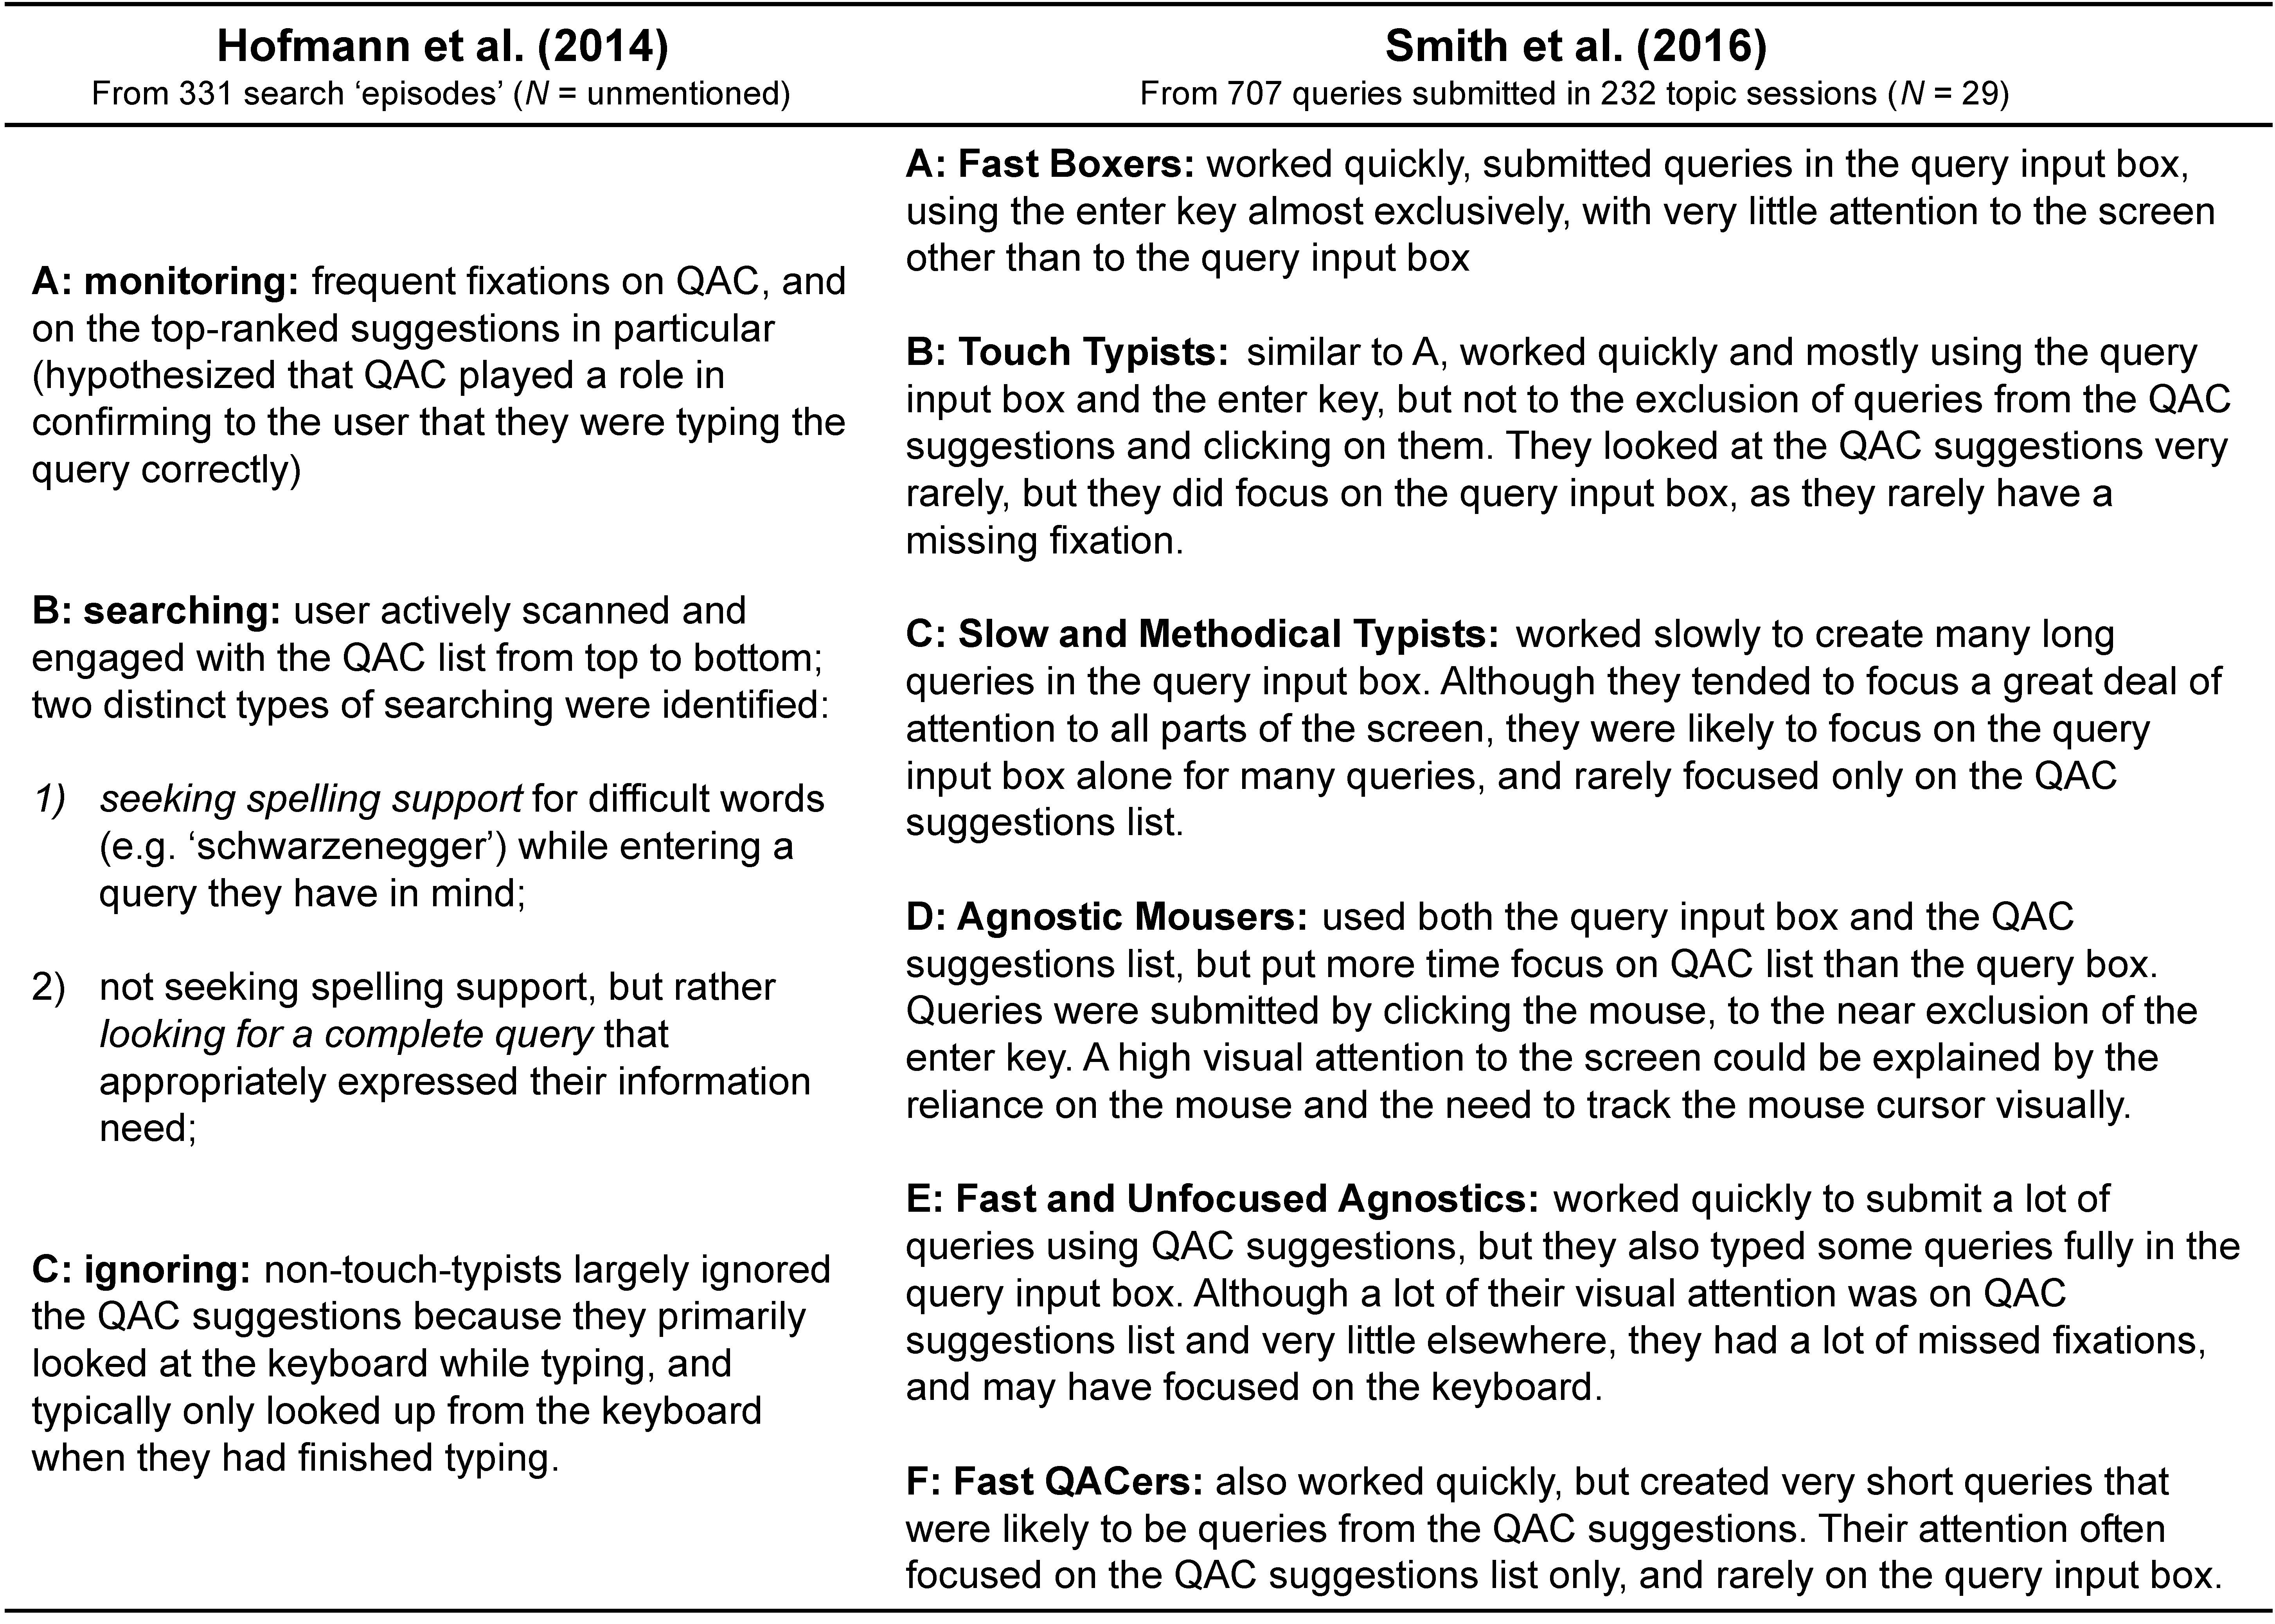
\includegraphics[width=1\linewidth]{figs/res-Q-QAC-profiles} 

}

\caption[Comparison of User behaviour profiles identified around Query Auto-Completion from eye-tracking data.]{Comparison of User behaviour profiles identified around Query Auto-Completion (QAC), from eye-tracking data, by Hofmann et al. (\protect\hyperlink{ref-125}{2014}) and Smith et al. (\protect\hyperlink{ref-129}{2016}).}\label{fig:res-Q-QAC-profiles}
\end{figure}





Several user behavioural profiles were identified by exploring
associations between visual attention from eye-tracking, search
interactions from mouse and keyboard activity, and the use of QAC
suggestions (\protect\hyperlink{ref-125}{Hofmann et al., 2014}; \protect\hyperlink{ref-129}{Smith et al., 2016}). These profiles are described in
Figure \ref{fig:res-Q-QAC-profiles}. An interesting, yet common-sense
observation was that participants' touch-typing ability greatly
influenced their interactions with QAC suggestions.

The native language of searchers was found to influence their overall
querying and searching behaviour. Ling et al. (\protect\hyperlink{ref-132}{2018}) explored this space using four
variations of a multi-lingual search interface. They observed that
participants strongly preferred to issue queries in their first or
native language. A second or non-native language was the next preferred
choice. Mixing of first and second-languages occurred very rarely. In
80\% of the total 300 tasks (25 users \(\times\) 4 interfaces \(\times\) 3
task-types), participants used a single language for querying. In the
rest 20\% of the tasks, participants switched languages for querying,
with a transition from first language to second language being the most
common.

\hypertarget{sec-bg-search-list}{%
\subsection{Stage 2: Search Results Evaluation / List-Item Selection}\label{sec-bg-search-list}}

\emph{How do users behave when examining a list of information-objects
(returned by an IR system)?}

After a user submits a query to an IR system, the next action they
generally perform is examining and evaluating the list of search results
returned by the IR system. In this section, we discuss empirical studies
which investigated information-searching behaviour around a list of
information-objects, or a representation of information-objects (also
called \emph{surrogates}). We identified some common themes in the research
questions investigated. The discussion below is grouped along these
themes, as relationships between search behaviour and: \emph{(i)} ranking of
search results; \emph{(ii)} information shown in search results; \emph{(iii)}
individual user characteristics; and \emph{(iv)} relevance judgement and
feedback.

\begin{figure}

{\centering 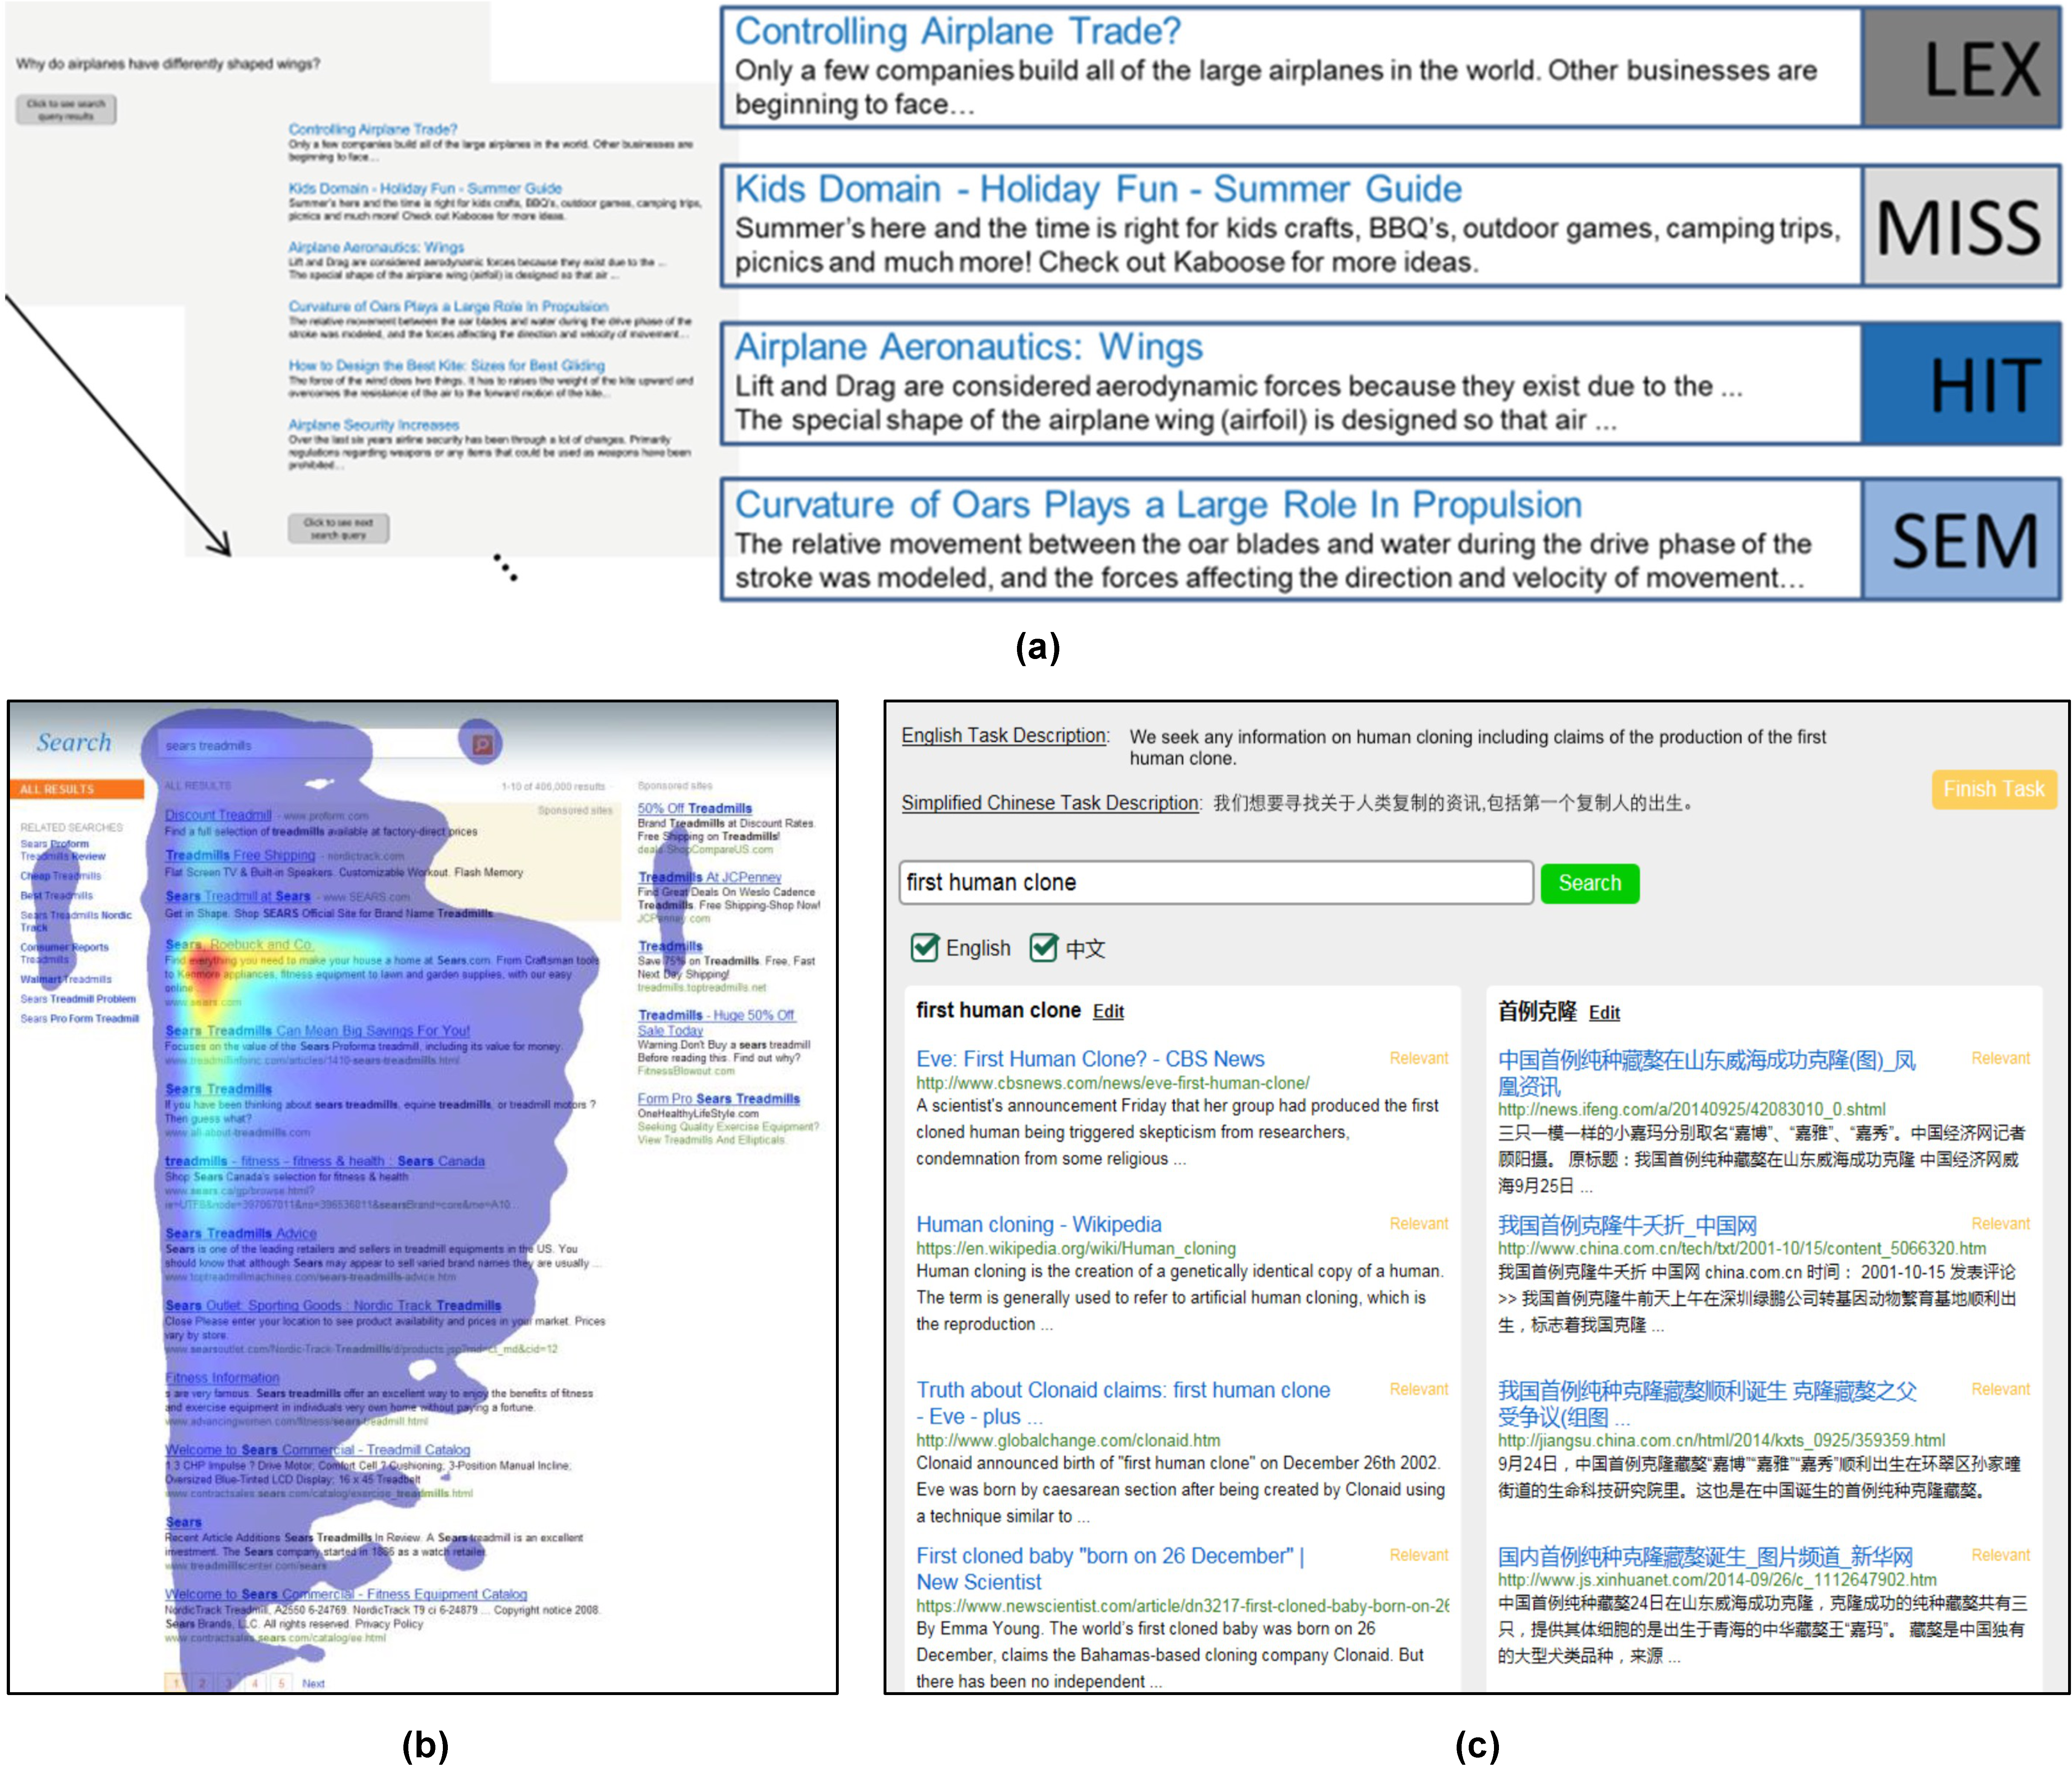
\includegraphics[width=1\linewidth]{figs/int-L-serp} 

}

\caption[Interfaces for studying user-interactions with search-engine results.]{Example interfaces for studying user-interactions with a search-engine results page (SERP): \textbf{(a)} a simplified SERP without query input facility, to judge relevance of search results (on a 4-level scale) for pre-determined search queries (in this case `why do airplanes have differently shaped wings?'), from Scharinger et al. (\protect\hyperlink{ref-63}{2016}); \textbf{(b)} eye-tracking heatmap on an organic SERP from Buscher et al. (\protect\hyperlink{ref-115}{2010}; \protect\hyperlink{ref-117}{Dumais et al., 2010}), showing the F-shaped pattern of visual attention; \textbf{(c)} a multilingual SERP from Ling et al. (\protect\hyperlink{ref-132}{2018}). This figure is best viewed in colour.}\label{fig:int-L-serp}
\end{figure}





\hypertarget{ranking-of-search-results}{%
\subsubsection{Ranking of search results}\label{ranking-of-search-results}}

Most search engines display results in a rank ordered list, with the
highest \emph{algorithmically} relevant results placed at the top, and others
results ordered below. Granka et al. (\protect\hyperlink{ref-101}{2004}; \protect\hyperlink{ref-108}{Lorigo et al., 2008}) studied eye-movement behaviour of
searchers examining SERPs, and reported observations from three user
studies. They saw that in 96\% of the queries, participants looked at
only the first result page, containing the top 10 results. No
participant looked beyond the third result page for a given query.
Participants looked primarily at the first few results, with nearly
equal attention (dwell time) given to the first and the second results.
However, despite equal attention, the first result was clicked 42\% of
the time, while the second was clicked only 8\% of the time. If none of
the top three results appeared to be relevant, then users chose not to
explore further results, but issued a reformulated query instead. When
the ranking of the search results were reversed (i.e.~placing less
relevant results in the higher ranked positions), participants spent
considerably more time scrutinizing and comparing results (more
fixations and regressions) before making a decision to click or
reformulate.

Some effects of gender were found to influence SERP examination (\protect\hyperlink{ref-108}{Lorigo et al., 2008}).
Females clicked on the second result twice as often, and made more
regressions or repeat viewings of already visited abstracts, compared to
males. Males were more likely to click on lower ranked results, from
entries 7 through 10, and also look beyond the first 10 results
significantly more often than women. Males were also more linear in
their scanning patterns, with less regressions. Pupil dilation did not
differ significantly between gender groups.

Effects of task-type and task-goals also influenced SERP examination
behaviour. Guan \& Cutrell (\protect\hyperlink{ref-105}{2007}) used Broder (\protect\hyperlink{ref-broder2002taxonomy}{2002})'s taxonomy of navigational vs.
informational searches. The authors reported that when users could not
find the target results for navigational searches, they either selected
the first result, or switched to a new query. However, for informational
searches, users rarely issued a new query and were more likely to try
out the top-ranked results, even when those results had lower relevance
to the task. This illustrated possible strong confidence of searchers in
the search engine's relevance ranking, even though searchers clearly saw
target results at lower positions. Thus, people were more likely to
deprecate their own sense of objective relevance and obeyed the ranking
determined by the search engine. Jiang et al. (\protect\hyperlink{ref-126}{2014}) used Li \& Belkin (\protect\hyperlink{ref-li2008faceted}{2008})'s framework of
search-tasks, and saw that in tasks having specific goals, searchers
fixated more on lower ranked results after some time. On the other hand,
for tasks having amorphous goals, there was a wider breadth in viewing
the SERP, and less effort spent in viewing the content pages. Fixations
tended to decrease as search session progressed, indicating decreased
interest and increasing mental effort, which could demonstrate
\emph{satisficing} behaviour (\protect\hyperlink{ref-simon1956rational}{Simon, 1956}). A comprehensive overview
of various behavioural traits associated with task-types and task-goals
can be found in (\protect\hyperlink{ref-126}{Jiang et al., 2014} Table 8).

\hypertarget{information-shown-in-search-results-surrogates}{%
\subsubsection{Information Shown in Search Results (Surrogates)}\label{information-shown-in-search-results-surrogates}}

The amount and quality of different kinds of information shown on SERPs
also affected user's information searching behaviour. Cutrell \& Guan (\protect\hyperlink{ref-104}{2007}) saw that as
the length of the surrogate information (result snippets) was increased,
user's search performance improved for informational tasks, but degraded
for navigational tasks (\protect\hyperlink{ref-broder2002taxonomy}{Broder, 2002}). Analyzing eye-tracking
data, they posited that the difference in performance was due to users
paying more attention to the snippet, and less attention to the URL
located at the bottom of the search result. This led to performance
deterioration in navigational searches. Buscher et al. (\protect\hyperlink{ref-115}{2010}) studied the effects of the
quality of advertisements placed in the SERPs (Figure \ref{fig:int-L-serp}(b)). Similar to findings discussed above, a
strong position bias of visual attention was found towards the top few
organic result entries --- the well known F-shaped pattern of visual
attention --- which was stronger for informational than for navigational
tasks. However, a strong bias \emph{against} sponsored links was observed in
general. Even for informational tasks, where participants generally had
a harder time finding a solution, the ads did not receive any additional
attention from the participants. Lorigo et al. (\protect\hyperlink{ref-108}{2008}) compared the visual attention
patterns of searchers using two different search engines: Google, and
Yahoo!. Behavioural trends followed similar patterns for both search
engines, even though Google was rated as the primary search engine of
all but one of the participants. They found slight variations in some
eye-tracking measures (reading time of surrogates, time to click
results, and query reformulation time), and some self-reported measures
(perceived ease of use, perceived satisfaction, and success rate).
However, none of these differences were statistically significant.

The novel query-preview interface by Qvarfordt et al. (\protect\hyperlink{ref-121}{2013}) was discussed in
Section~\ref{sec-bg-search-query} and in
Figure~\ref{fig:int-Q}(a).
The authors also reported several observations about user behaviour on
SERPs. They saw that the presence of the preview visualization enabled
participants to look deeper into the results lists. Participants tried
to use the preview as a navigation tool, although it was not designed as
such. The tool increased the rates at which participants examined
documents at middle ranks in query results, and thus helped discover
more useful documents in those middle ranks than without the preview
widget. The preview tool also helped to increase the diversity of
documents found in a search session, which could in turn lead to better
performance in terms of recall and precision. Thus, the tool helped
searchers overcome the strong position bias towards top-ranked results,
as observed by other studies discussed previously.

\begin{figure}

{\centering 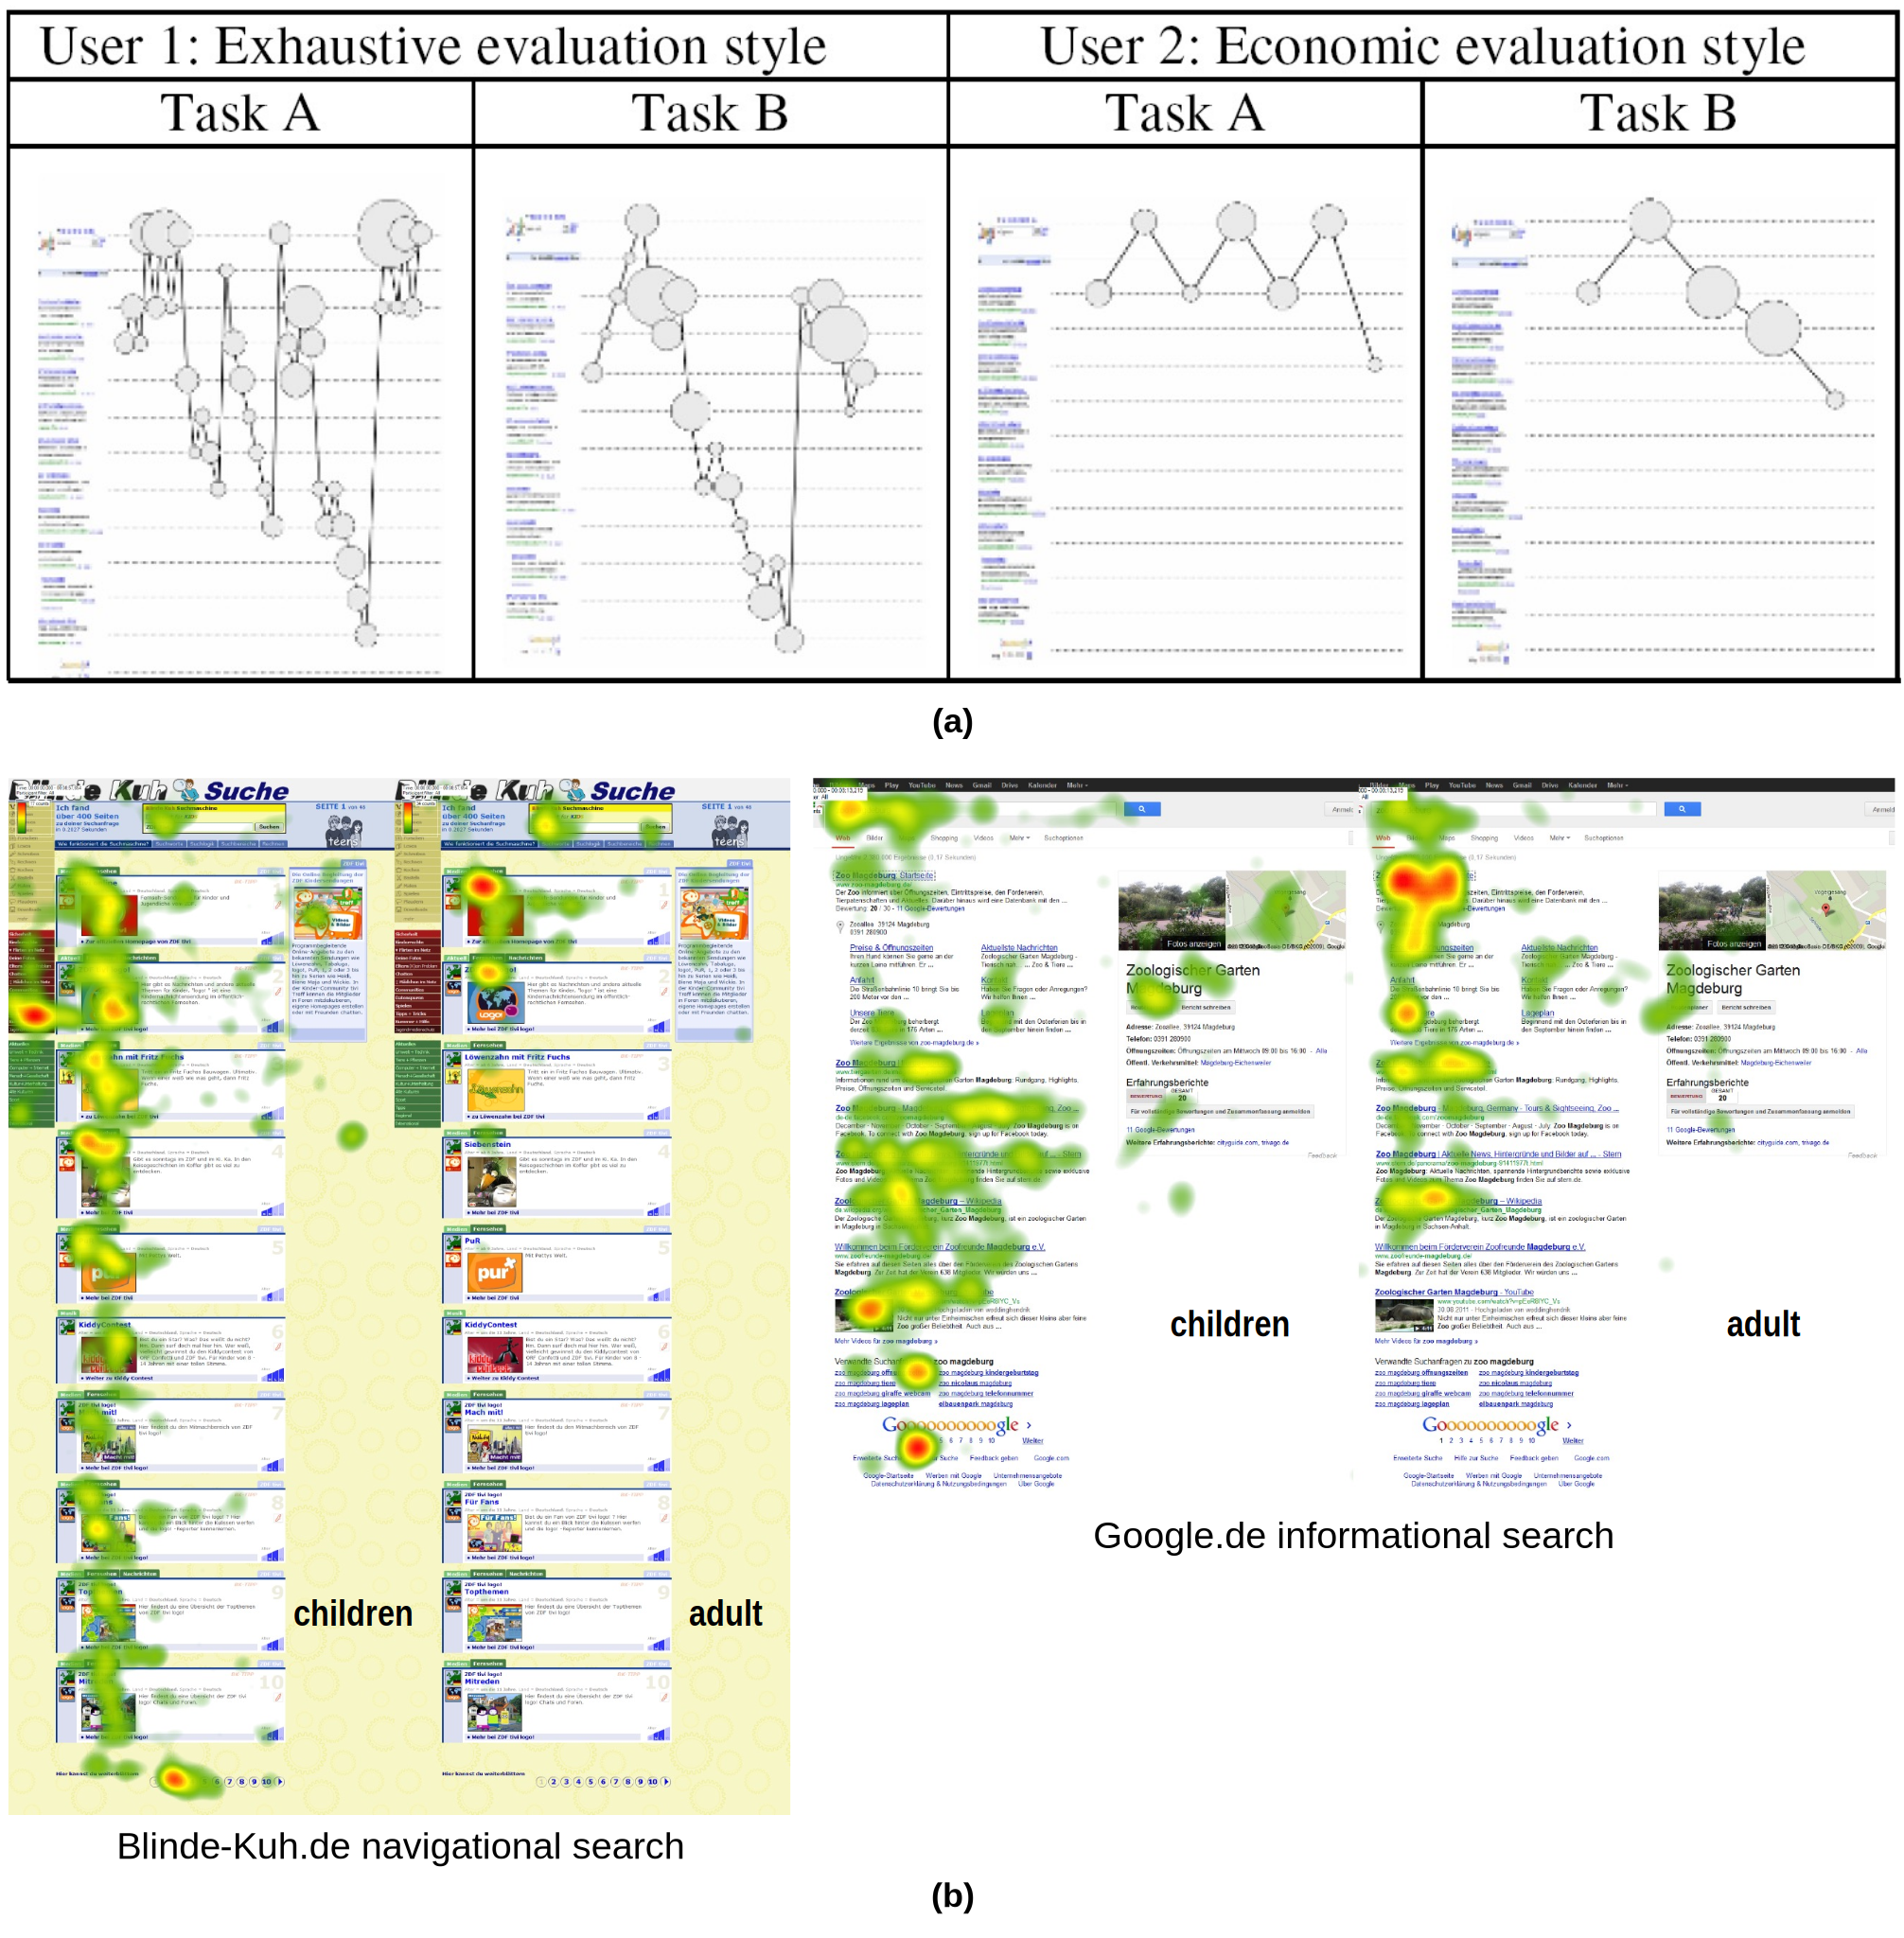
\includegraphics[width=1\linewidth]{figs/res-L-serp-user-chars} 

}

\caption[Differences in user characteristics on interactions with SERPs.]{Effects of differences in user characteristics on interactions with SERPs: \textbf{(a)} exhaustive or \emph{depth-first} user (User 1), vs.~economic or \emph{breadth-first} user (User 2), examining mostly irrelevant results in Task A, and mostly relevant results in Task B (both users followed the second link in Task B); vertical axis denotes vertical location on SERP, and horizontal axis denotes temporal ordering of result examination; from Aula et al. (\protect\hyperlink{ref-102}{2005}); (similar patterns were identified by Bilal \& Gwizdka (\protect\hyperlink{ref-139}{2016}), in the SERP examination behaviour of children) \textbf{(b)} children vs.~adults examining SERPs from a German search engine for children (left), and Google (right); differently from adults, children exhaustively explored all search results, paid more attention to thumbnails and embedded media, and read less text-only snippets; from Gossen et al. (\protect\hyperlink{ref-124}{2014}). Similar observations as with children were reported for searchers with dyslexia (\protect\hyperlink{ref-palani2020eye}{Palani et al., 2020}). This figure is best viewed in colour.}\label{fig:res-L-serp-user-chars}
\end{figure}





\hypertarget{individual-user-characteristics}{%
\subsubsection{Individual User Characteristics}\label{individual-user-characteristics}}

Individual traits of searchers also influence their pattern of
interactions with a SERP, and these patterns can be revealed by
analyzing eye-tracking data. For instance, searchers have been
classified as \emph{economic} vs.~\emph{exhaustive}, based on their style of
evaluating SERPs (\protect\hyperlink{ref-102}{Aula et al., 2005}). \emph{Economic} searchers were found to scan less
than half (three) of the displayed results above the fold, before making
their first action (query re-formulation, or following a link).
\emph{Exhaustive} searchers evaluated more than half of the visible results
above the fold, or even scrolled the results page to view all of the
results, before performing the first action. Thus, economic searchers
demonstrated depth-first search strategy, while exhaustive users
favoured the breadth-first approach
(Figure~\ref{fig:res-L-serp-user-chars}(a)). Dumais et al. (\protect\hyperlink{ref-117}{2010}) demonstrated the use of
unsupervised clustering to re-identify the \emph{economic}-\emph{exhaustive} user
groups, based on differences in total fixation impact \footnote{
  a measure derived from eye fixation durations, proposed by Buscher et al. (\protect\hyperlink{ref-110}{2009})}, scanpaths,
task outcomes, and questionnaire data. The \emph{economic} cluster was
further broken down by users who looked primarily at results
(\emph{economic-results} cluster), and users who viewed both results and ads
(\emph{economic-ads} cluster). All three groups spent the highest amount of
time on the first three results, with the \emph{exhaustive} group being
substantially slower than the other two groups. The \emph{exhaustive} and
\emph{economic-results} groups spent the second-highest amount of time on
results four through six, while the \emph{economic-eds} group spent this time
on the main advertisements. This group spent more than twice as much
time on the main ads as the \emph{economic-results} group, and even more time
on main ads than the \emph{exhaustive group}. This observation is incongruent
to Buscher et al. (\protect\hyperlink{ref-115}{2010})`s findings, as they observed a generally strong bias \emph{against}
viewing sponsored links. Abualsaud \& Smucker (\protect\hyperlink{ref-135}{2019}) conducted further analysis using these
user types, and, in general, reconfirmed the previous findings. They
found that the results above the fold, especially, \textbf{\emph{the first three
search results are special}}, more so for economic users. On submitting
a 'weak' query, if economic users did not find a correct result within
the first three results, they abandoned examination, and reformulated
their query.

Age of searchers also influence SERP evaluation behaviour. Gossen et al. (\protect\hyperlink{ref-124}{2014})
demonstrated differences in SERP evaluation for children and adults
(Figure~\ref{fig:res-L-serp-user-chars}(b)). When answers were not found
within the top search results, the adults reformulated the query
starting a new search, while young users exhaustively explored all the
ten results, and used the navigation buttons between results pages to
continue further examination. Children also paid more attention to
thumbnails and embedded media, and focused less on textual snippets.
Children saw the query suggestions at the bottom of the Google SERP
(because they navigated to the bottom), while the adults did not. Bilal \& Gwizdka (\protect\hyperlink{ref-139}{2016}; \protect\hyperlink{ref-140}{Gwizdka \& Bilal, 2017}) investigated this phenomenon further, and observed that even
within children, age plays a role in SERP evaluation behaviour. Younger
children (grade six, age 11) clicked more often on results in
lower-ranked positions than older children (grade eight, age 13). Older
children's clicking behaviour was based more often on reading result
snippets, and not just on the ranked position of a result in a SERP.
Whereas, younger children made less deliberate choices in choosing which
result to click, and were more exhaustive in the exploration of results.
Thus, using Aula et al. (\protect\hyperlink{ref-102}{2005})'s classification and Dumais et al. (\protect\hyperlink{ref-117}{2010})'s observations, it can be
posited that (younger) children start out as \emph{exhaustive} searchers.
With increase in age and maturity, older children and adults evolve into
\emph{economic} searchers. Interestingly, very similar behaviour patterns as
with children (scrolling further down on SERPs, exhaustive exploration,
etc.) were also observed recently for searchers with dyslexia
(\protect\hyperlink{ref-palani2020eye}{Palani et al., 2020}).

Searcher's native language also influenced SERP interaction behaviour
(\protect\hyperlink{ref-132}{Ling et al., 2018}) (Figure~\ref{fig:int-L-serp}(c)). We discussed in
Section~\ref{sec-bg-search-query} that users strongly preferred issuing
queries in a single language, especially their native language. However,
while examining SERPs, they marked search results in both their first
language and second language to be relevant, to an equal degree. This
confirms the usefulness of search result pages that integrate results
from multiple languages. However, a clear separation in the language of
the search results was strongly preferred, and an `interleaved'
presentation (e.g.~odd numbered results in one language and even
numbered results in another language) was least preferred.

\begin{figure}

{\centering \includegraphics[width=1\linewidth]{figs/int-L-serp-new-vertical} 

}

\caption[Examples of Google SERP going beyond the ``ten blue links'' paradigm.]{Google search engine result page (SERP) for the queries: \textbf{(a)} ``coronavirus'' \textbf{(b)} ``toyota'' \textbf{(c)} ``evaporation'', and \textbf{(d)} ``life of pie''. All screenshots are from `above-the-fold', viewed on a \(2560 \times 1440\) monitor. These examples highlight that modern SERPs have come a long way from a list of ``ten blue links''. SERPs are becoming consumable information-objects in their own right, and thus require different kinds of cognitive processing and interactions, than from the early days of the internet. Inspired and adapted from Wang et al. (\protect\hyperlink{ref-yue2018optimizing}{2018}). Accessed on May 5, 2020. This figure is best viewed in colour.}\label{fig:int-L-serp-new-vertical}
\end{figure}





\hypertarget{relevance-judgement}{%
\subsubsection{Relevance Judgement}\label{relevance-judgement}}

Balatsoukas \& Ruthven (\protect\hyperlink{ref-114}{2010}, \protect\hyperlink{ref-119}{2012}) proposed a list of relevance criteria for understanding
how searchers evaluate search results, or perform \emph{relevance judgement}.
These criteria were developed based on literature reviews and their
empirical findings from eye-tracking studies. The final list contains 15
relevance criteria (e.g., \emph{topicality}, \emph{quality}, \emph{recency}, \emph{scope},
\emph{availability}, etc.) and can be found in (\protect\hyperlink{ref-119}{Balatsoukas \& Ruthven, 2012} Appendix B).

Search engines are increasingly adding different modalities of
information on the SERP, besides the ``ten blue links''. These include
images, videos, encyclopaedic information, and maps
(Figure~\ref{fig:int-L-serp-new-vertical}). Z. Liu et al. (\protect\hyperlink{ref-128}{2015}) studied the influence of
these different forms of SERP information -- called `verticals' -- on
searcher's relevance judgements. A general observation was that if
verticals were present in a SERP, they created strong attraction biases.
The attraction effect was influenced by the type of verticals, while the
vertical quality (relevant or not) did not have a major impact. For
instance, `images' and `software download' verticals had higher visual
attention, while news verticals had equal attention as the ``ten blue
links'' search results.

\hypertarget{sec-bg-search-content-page}{%
\subsection{Stage 3: Content Page Evaluation / Item Examination}\label{sec-bg-search-content-page}}

\begin{quote}
\emph{How do users behave when examining a single information-object (e.g., a
a non-search-engine webpage, aka content page) obtained from an IR
system?}
\end{quote}

In online information searching, searchers repeatedly interact with
individual webpages, a.k.a. `content pages' in IR terminology. These
webpages can be visited by following links from a search engine,
following links between different webpages, or directly typing the URL
in the browser.

The first group of papers we discuss investigated users' \textbf{visual
attention} and \textbf{reading behaviour} on webpages. Pan et al. (\protect\hyperlink{ref-pan2004determinants}{2004})
studied whether eye-tracking scanpaths on webpages varied based on
task-type, webpage type (business, news, search, or shopping), viewing
order of webpages, and gender of users. The found significant
differences for all factors, except for task-type, which seemed to have
no effect on scanpaths. They used weak task-types: remembering what was
on a webpage vs.~no specific task. In a later work on using
informational vs.~navigational search-tasks, they again saw limited
effect of task-type on visual attention (\protect\hyperlink{ref-lorigo2006influence}{Lorigo et al., 2006}). Findings
from Josephson \& Holmes (\protect\hyperlink{ref-josephson2002visual}{2002})'s study suggested that users possibly follow
habitually preferred scanpaths on a webpage, which can be influenced by
factors like webpage characteristics and memory. However, they used only
three webpages, making the findings difficult to generalize.
Goldberg et al. (\protect\hyperlink{ref-goldberg2002eye}{2002}) studied eye movements on Web portals during
search-tasks, and saw that header bars were typically not viewed before
focusing the main part of the page. So they suggested placing navigation
bars on the left side of a page. Beymer et al. (\protect\hyperlink{ref-beymer2007eye}{2007}) focused on a very
specific feature on webpages: images that are placed next to text
content and how they influence eye movements during a reading task. They
found significant influence on fixation location and duration. Those
influences were dependent on how the image contents related to the text
contents (i.e., whether they showed ads or text-related images). Buscher et al. (\protect\hyperlink{ref-110}{2009})
presented findings from a large scale study where users performed
information-foraging and page-recognition tasks. They observed that in
the first few moments, users quickly scanned the top left of the page,
presumably looking for clues about the content, provenance, type of
information, etc. for that page. The elements that were normally
displayed in the upper left third of webpages (e.g., logos, headlines,
titles or perhaps an important picture related to the content) seemed to
be important for recognizing and categorizing a page. After these
initial moments, influence of task-type set in. For page-recognition
tasks, the attention remained in the top-left corner of the webpage.
However, for information-foraging tasks, fixations moved to the
center-left region of the webpage, where the user was possibly trying to
find task-specific information. The right third of webpages attracted
almost no visual attention during the first one-second of each page
view. Afterwards as well, most users seemed to entirely ignore this
region, or only occasionally look at it. This suggested that users had
low expectations of information-content or general relevance on the
right side of most webpages. As many webpages display advertisements on
the right side, this was a plausible observation, and are in line with
the observed ``F-shaped-patterns'' \footnote{
  \url{https://www.nngroup.com/articles/f-shaped-pattern-reading-web-content}} on webpages.

Buscher et al. (\protect\hyperlink{ref-110}{2009}) also proposed an eye-tracking measure called \emph{fixation impact}.
This measure first appends a circular Gaussian distribution around each
fixation on a webpage element, to create a fuzzy area of interest. This
is called the \emph{distance impact} value. If a webpage element completely
covers the fixation circle (Gaussian distribution), it gets a \emph{distance
impact} value of 1. If the element partially covers the fixation circle,
its \emph{distance impact} value is smaller. Multiplying the \emph{distance
impact} value with the fixation duration gives the fixation impact for
the given webpage element. Thus, an element that completely covers the
fixation circle gets the full fixation duration as \emph{fixation impact}
value. Elements which are partially inside the circle get a value
proportional to the Gaussian distribution. The authors posited that the
rationale behind creating the fixation impact measure was motivated by
observations from human vision research, which indicates that fixation
duration correlates with the amount of visual information processed; the
longer a fixation, the more information is processed around the fixation
centre. Using the fixation impact measure, Buscher et al. (\protect\hyperlink{ref-110}{2009}) proposed a model for
predicting the amount visual attention that individual webpage elements
may receive (i.e.~visual salience).

Another group of studies investigated how users judged \textbf{relevance of
webpages} w.r.t. an assigned search-task or information need.
(\protect\hyperlink{ref-74}{Gwizdka, 2018}; \protect\hyperlink{ref-47}{Gwizdka \& Zhang, 2015a}, \protect\hyperlink{ref-48}{2015b}) observed that when relevant pages were revisited, the
webpages were read more carefully. Pupil dilations were significantly
larger on visits and revisits to relevant pages, and just before
relevance judgements were made. Certain conditions of visits and
revisits also showed significant differences in EEG alpha frequency band
power, and EEG-derived attention levels. Relevance of individual webpage
elements were also assessed as \emph{click-intention}: whether users would
click on an element they were looking at. Slanzi et al. (\protect\hyperlink{ref-69}{2017}) used pupillometry and EEG
signals to predict whether a mouse click was present for each eye
fixation. EEG features included simple statistical features of signals
(mean, SD, power, etc.), as well as sophisticated mathematical features
(Hjorth features, Fractal Dimensions, Entropy, etc.). A battery of
classifier models were tested. However, the results were not promising.
Logistic Regression had the highest accuracy (71\%), but very low F1
score (0.33), while neural network based classifiers the had highest F1
score (0.4). The authors suspected that the low sampling rate of their
instruments (30 Hz eye-tracker and 128 Hz 14-channel EEG) impacted their
classifier performances. González-Ibáñez et al. (\protect\hyperlink{ref-81}{2019}) compared relevance prediction performances
in the presence and absence of eye-tracking data, and argued that when
eye-tracking data collection is not feasible, mouse left-clicks can be
used a good alternative indicator of relevance.

The `\emph{Competition for Attention}' theory states that items in our visual
field compete for our attention (\protect\hyperlink{ref-desimone1995neural}{Desimone \& Duncan, 1995}). Djamasbi et al. (\protect\hyperlink{ref-30}{2013}) studied web
search and browsing from the perspective of this theory. Theoretical
models suggest that in goal-directed searches, information-salience
and/or information-relevance drives search behaviour (i.e.~competition
for attention does not hold true), whereas exploratory search behaviour
is influenced by competition among stimuli that attracts a user's
attention (i.e.~competition for attention holds true). However, in
practice, information search behaviour often becomes a combination of
both types of visual search activities (\protect\hyperlink{ref-groner1984looking}{Groner et al., 1984}). Djamasbi et al. (\protect\hyperlink{ref-30}{2013}) found
that, despite the goal directed nature of their search-task (finding the
best snack place in Boston to take their friends) \emph{competition for
attention} had some effect at the content page level. Some of the users'
attention was diverted to non-focal areas on content pages. However,
there was little effect of \emph{competition for attention} on how the
results were viewed on SERPs. Users exhibited the familiar top-to-bottom
pattern of viewing
(Section~\ref{sec-bg-search-list}), paying the most attention to the top
two entries.

\hypertarget{sec-bg-search-expertise}{%
\section{Effects of Expertise and Working Memory on Search Behaviour}\label{sec-bg-search-expertise}}

\begin{figure}

{\centering 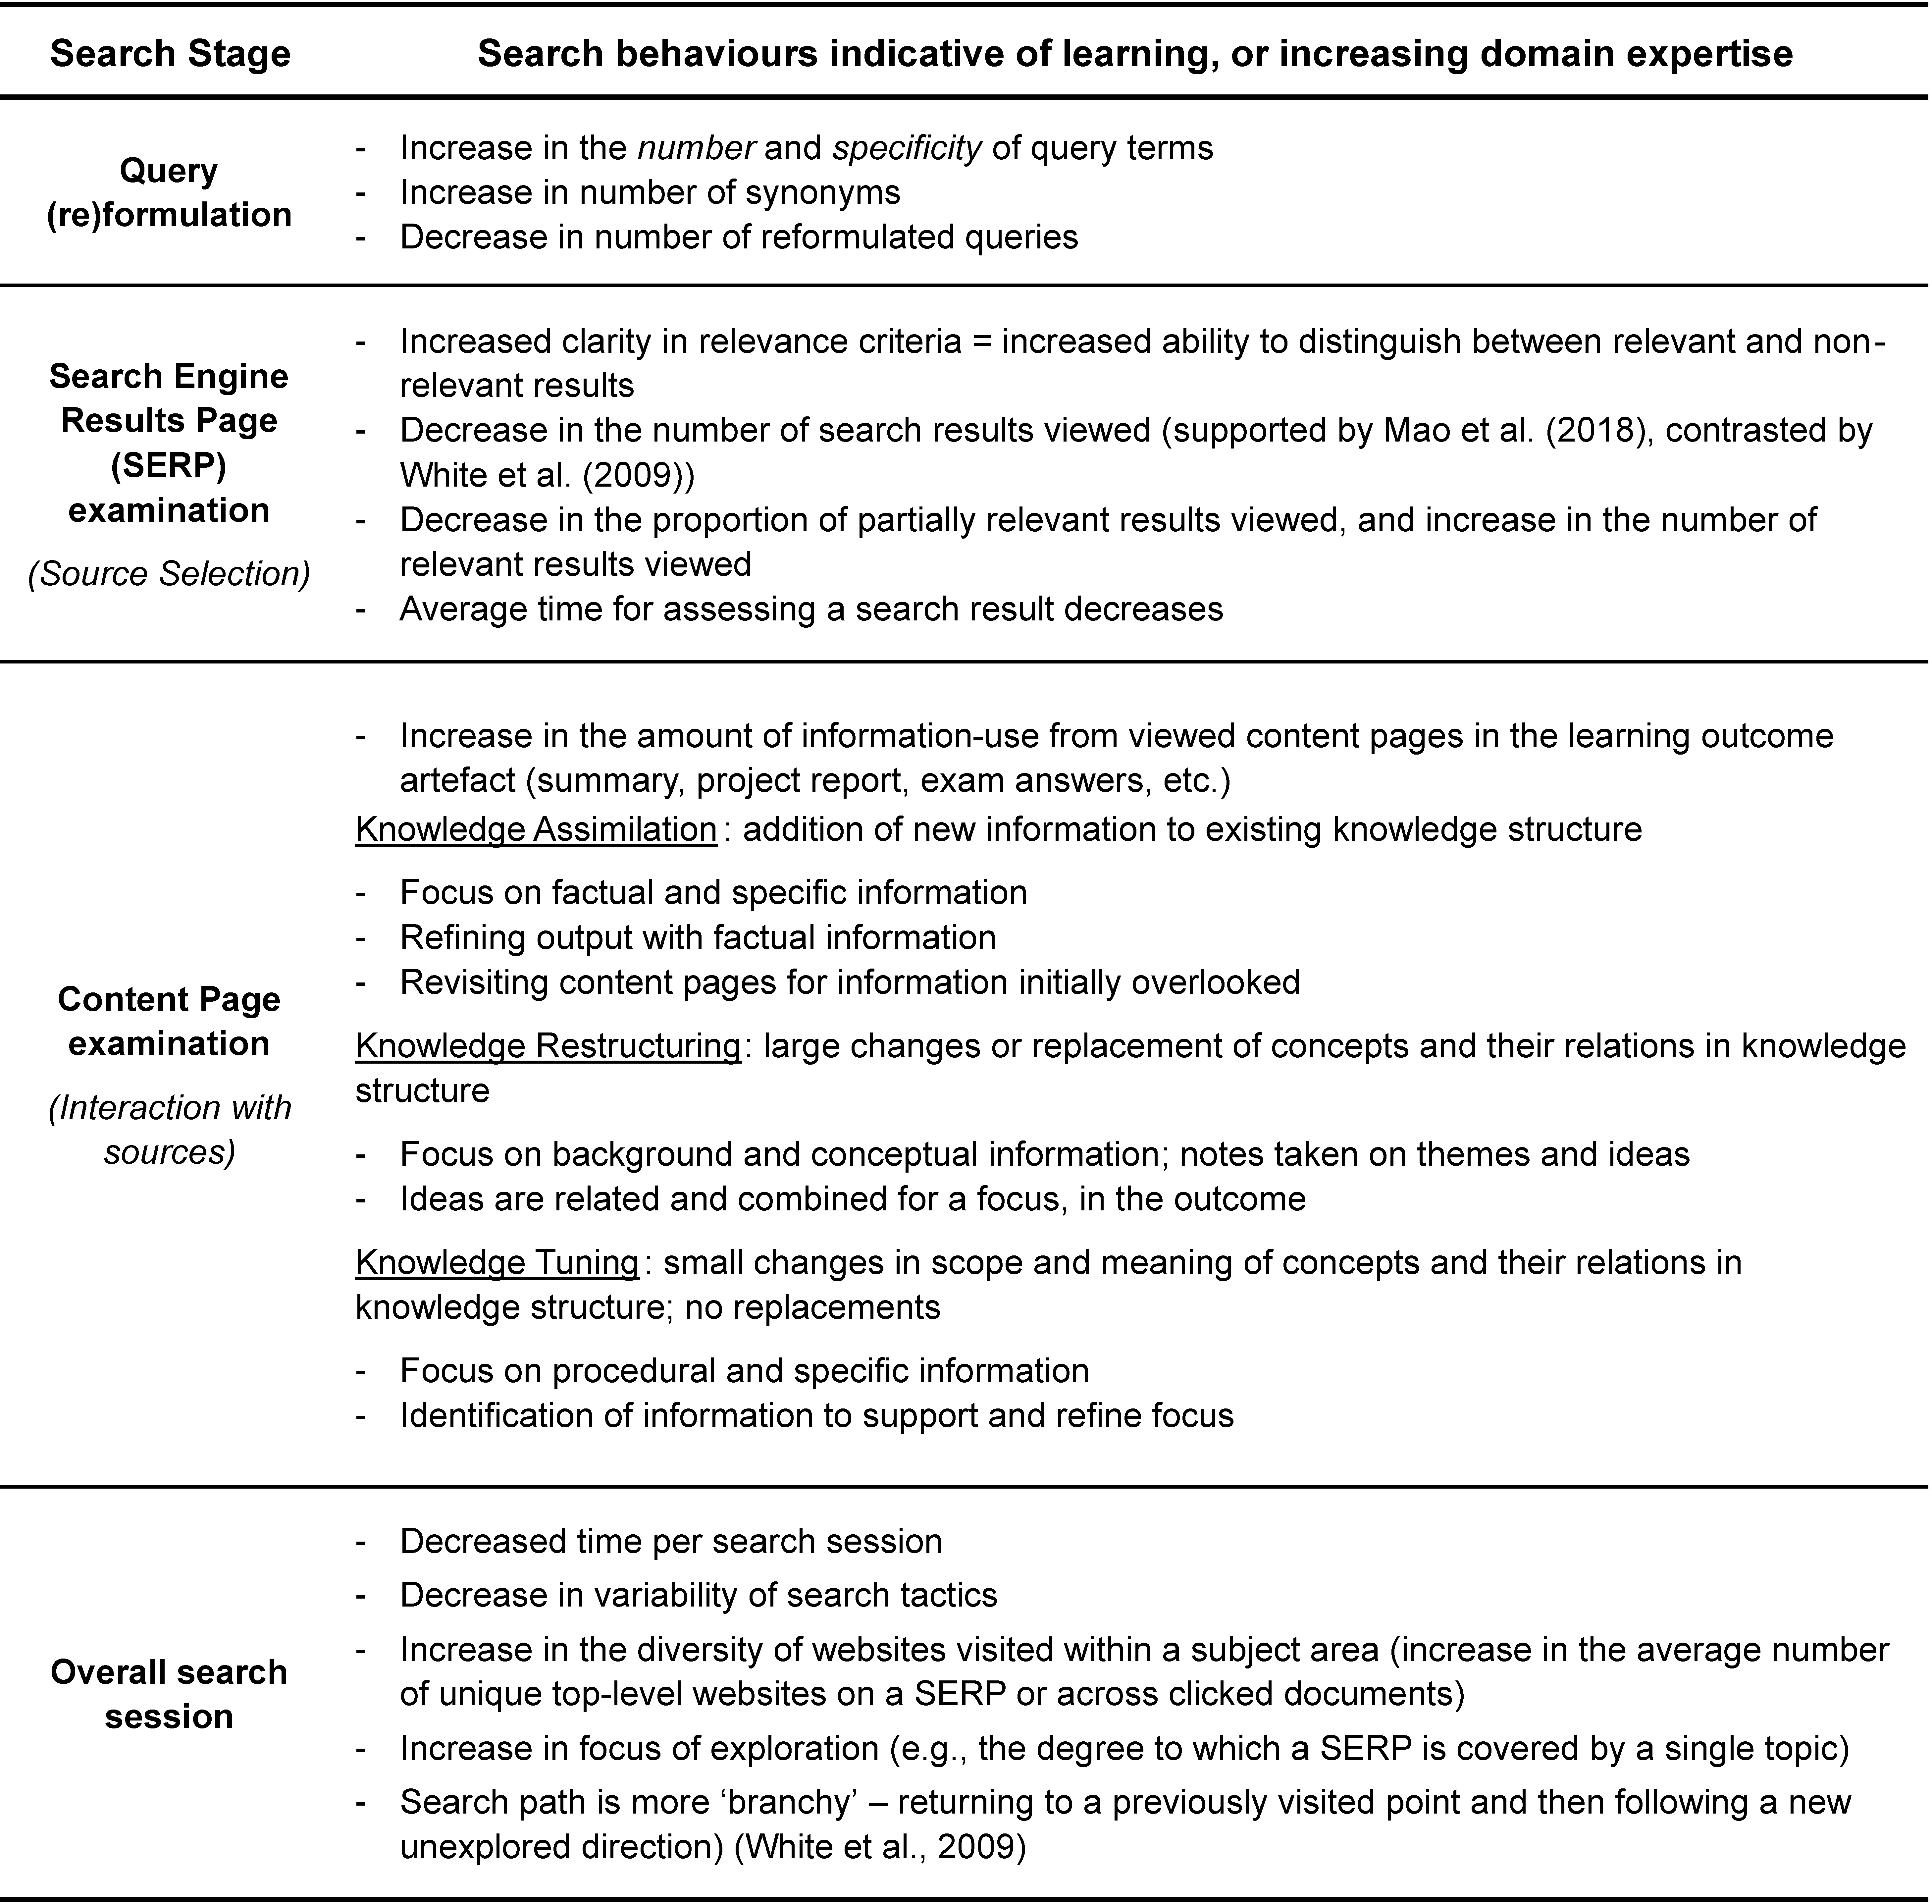
\includegraphics[width=1\linewidth]{figs/search-behaviours} 

}

\caption[Components of metacognition.]{Literature reviews by Rieh et al. (\protect\hyperlink{ref-rieh2016searching}{2016}) and Vakkari (\protect\hyperlink{ref-vakkari2016searching}{2016}) identified the following search behavioural traits as indicative of domain experts, or novices undergoing learning to become experts.}\label{fig:search-behaviours}
\end{figure}





Our focus of discussion in this dissertation is information searching and
learning. As we saw in Chapter \ref{ch-bg-learn}, learning and expertise are closely connected:
expertise is an evolving characteristic of users that reflects learning
over time, rather than being a static property
(\protect\hyperlink{ref-rieh2016searching}{Rieh et al., 2016}; \protect\hyperlink{ref-sawyer2005cambridge}{Sawyer, 2005}). (\protect\hyperlink{ref-white2016interactions}{White, 2016a, Chapter 7}) considers three types of expertise, that are relevant in
information seeking settings: \emph{(i)} domain or subject-matter expertise;
\emph{(ii)} search expertise; and \emph{(iii)} task expertise. \textbf{Domain or
subject-matter expertise} describes people's knowledge in a specialised
subject area such as a domain of interest. \textbf{Search expertise} refers
to people's skill level at performing information-seeking activities,
both in a Web search setting and in other settings such as specialised
domains. \textbf{Task expertise} describes people's expertise in performing
particular search tasks, potentially independent of domain. Although
considered distinctly, the boundaries between these expertise types are
quite blurred, and therefore difficult to estimate at the time of
search, and model it in a way that can be consumed by search systems.

Previous work on domain knowledge and expertise have linked \footnote{and continue to link} domain
expertise and search behaviour in terms of metrics, behavioural
patterns, and criteria
(\protect\hyperlink{ref-cole2013inferring}{M. J. Cole et al., 2013}; \protect\hyperlink{ref-133}{Mao et al., 2018}; \protect\hyperlink{ref-o2020role}{O'Brien et al., 2020}; \protect\hyperlink{ref-white2009characterizing}{White et al., 2009}). A
representative summary is presented in Figure \ref{fig:search-behaviours}, and is adapted from literature
reviews by (\protect\hyperlink{ref-rieh2016searching}{Rieh et al., 2016}) and (\protect\hyperlink{ref-vakkari2016searching}{Vakkari, 2016}). Briefly,
(\protect\hyperlink{ref-wildemuth2004effects}{Wildemuth, 2004}) showed that novices converge toward the same
search patterns as experts, as they are exposed to a topic and learn
more about it. (\protect\hyperlink{ref-zhang2011predicting}{X. Zhang et al., 2011}) found that features such as
document retention, query length, and the average rank of results
selected could be predictive of domain expertise. (\protect\hyperlink{ref-cole2013inferring}{M. J. Cole et al., 2013})
showed that eye-gaze patterns could be used to predict an individual's
level of domain expertise using estimates of cognitive effort associated
with reading. (\protect\hyperlink{ref-white2009characterizing}{White et al., 2009}) showed that measures such as
diverse website visitation, more narrow topical focus, less diversity
(or entropy), more `branchiness' of search sessions, less dwell time,
and higher query and session complexity are indicative of expert
knoweldge and/or search behaviour.

As a stark contrast, (\protect\hyperlink{ref-zlatkin2021students}{Zlatkin-Troitschanskaia et al., 2021}) reviewed literature on
higher education \textbf{students' information search behaviour}. Students
can be considered as novices in all three respects:
domain/subject-matter, search skills, and task. The authors report that
across literature, higher education students' information search
behaviour tends to follow some general general patterns: \emph{(i) foraging:}
no explicit (task-specific) research plan and little understanding of
the differences (pros/cons) between various IR systems; \emph{(ii) Google
dependence:} no intention to use any search tool other than Google,
causing students to struggle to understand library information
structures and engage with scholarly literature effectively; \emph{(iii)
rudimentary search heuristic:} reliance on one and the same simple
search strategy, regardless of search context; \emph{(iv) habitual topic
changing:} students change the search topic after rather superficial
skimming, and before evaluating all search results; and \emph{(v) overuse of
natural language:} students type questions into the search box that are
phrased as if posing them to a person. Highly ranked online sources
accessed via a well-known search engine were perceived as trustworthy.

Effects of memory span and working memory capacity have also been found
to influence search effort and search behaviour
(\protect\hyperlink{ref-arguello2019effects}{Arguello \& Choi, 2019}; \protect\hyperlink{ref-CHIIR19}{Bhattacharya \& Gwizdka, 2019a}; \protect\hyperlink{ref-cole2020more}{L. Cole et al., 2020}; \protect\hyperlink{ref-gwizdka2013effects}{Gwizdka, 2013}, \protect\hyperlink{ref-gwizdka2017can}{2017}).
\textbf{Working memory} (WM) is considered a core executive function is
defined as someone's ability to hold information in short-term memory
when it is no longer perceptually present
(\protect\hyperlink{ref-diamond2013executive}{Diamond, 2013}; \protect\hyperlink{ref-miller1956magical}{G. A. Miller, 1956}). (\protect\hyperlink{ref-bailey2011amount}{Bailey \& Kelly, 2011}) showed
that the amount of effort was a good indicator of user success on search
tasks. (\protect\hyperlink{ref-smith2008user}{Smith \& Kantor, 2008}) studied searcher adaptation to poorly performing
systems and found that searchers changed their search behaviors between
difficult and easy topics in a way that could indicate that users are
satisficing. Differences in search effort between different types
systems (higher effort invested in searching library database vs.~web)
were found by (\protect\hyperlink{ref-rieh2012amount}{Rieh et al., 2012}). A couple of studies showed that mental
effort involved in judging document relevance is lower for irrelevant
and higher for relevant documents (\protect\hyperlink{ref-37}{Gwizdka, 2014}; \protect\hyperlink{ref-villa2013relevance}{Villa \& Halvey, 2013}).
(\protect\hyperlink{ref-gwizdka2017can}{Gwizdka, 2017}) found that that higher WM searchers perform more
actions and that most significant differences are in time spent on
reading results pages. Behaviour of high and low WM searchers were also
found to change differently in the course of a search task performance.

\hypertarget{assessing-learning-during-search}{%
\section{Assessing Learning during Search}\label{assessing-learning-during-search}}

In order for IR systems to foster user-learning at scale, while
respecting individual differences of searchers, there is a need for
measures to represent, assess, and evaluate the learning process,
possibly in an automated fashion. Consequently, a variety of assessment
tools have been used in prior studies. These include self reports, close
ended factual questions (multiple choice), open ended questions (short
answers, summaries, essays, free recall, sentence generation), and
visual mapping techniques using concept maps or mind maps. Each approach
has its own associated advantages and limitations.
Urgo \& Arguello (\protect\hyperlink{ref-urgo2022learning}{2022}) compare and contrast these assessment techniques extensively in their very comprehensive literature review.

\textbf{Self-report} asks
searchers to rate their self-perceived pre-search and post-search
knowledge levels (\protect\hyperlink{ref-ghosh2018SearchingLearningExploring}{Ghosh et al., 2018}; \protect\hyperlink{ref-o2020role}{O'Brien et al., 2020}).
This approach is the easiest to construct, and can be generalised over
any search topic. However, self-perceptions may not objectively
represent true learning. \textbf{Closed ended questions} test searchers'
knowledge using factual multiple choice questions (MCQs). The answer
options can be a mixture of fact-based responses (\emph{TRUE}, \emph{FALSE}, or \emph{I
DON'T KNOW}),
(\protect\hyperlink{ref-gadiraju2018AnalyzingKnowledgeGain}{Gadiraju et al., 2018}; \protect\hyperlink{ref-xu2020does}{Xu et al., 2020}; \protect\hyperlink{ref-yu2018PredictingUserKnowledgea}{Yu et al., 2018})
or recall-based responses (\emph{I remember / don't remember seeing this
information}) (\protect\hyperlink{ref-kruikemeier2018learning}{Kruikemeier et al., 2018}; \protect\hyperlink{ref-roy2020exploring}{Roy et al., 2020}).
Constructing topic-dependant MCQs may take time and effort, since they
are topic dependant. Recent work on automatic question generation may be
leveraged to overcome this limitation (\protect\hyperlink{ref-syed2020improving}{Syed et al., 2020}). Evaluating
close ended questions is the easiest, and generally automated in various
online learning platforms. Multiple choice questions, however, suffer
from a limitation: they allow respondents to answer correctly by
guesswork. \textbf{Open ended questions} assess learning by letting searchers
write natural language summaries or short answers
(\protect\hyperlink{ref-bhattacharya2018relating}{Bhattacharya \& Gwizdka, 2018}; \protect\hyperlink{ref-o2020role}{O'Brien et al., 2020}; \protect\hyperlink{ref-roy2021note}{Roy et al., 2021}). Depending on
experimental design, prompts for writing such responses can be generic
(least effort) (\protect\hyperlink{ref-bhattacharya2018relating}{Bhattacharya \& Gwizdka, 2018}, \protect\hyperlink{ref-bhattacharya2019measuring}{2019b}),
or topic-specific (some effort) (\protect\hyperlink{ref-syed2020improving}{Syed et al., 2020}). While this
approach can provide the richest information about the searcher's
knowledge state, evaluating such responses is the most challenging, and
requires extensive human intervention
(\protect\hyperlink{ref-kanniainen2021assessing}{Kanniainen et al., 2021}; \protect\hyperlink{ref-leu2015new}{Leu et al., 2015}; \protect\hyperlink{ref-wilson2013comparison}{M. J. Wilson \& Wilson, 2013}) (as
discussed in Section \ref{sec-bg-learn-artefact}). \textbf{Visual mapping} techniques such
as mind maps and concept maps have also been used to assess learning
during search
(\protect\hyperlink{ref-egusa2010usingb}{Egusa et al., 2010}, \protect\hyperlink{ref-egusa2014howd}{2014a}, \protect\hyperlink{ref-egusa2014howe}{2014b}, \protect\hyperlink{ref-egusa2017evaluating}{2017}; \protect\hyperlink{ref-halttunen2005assessing}{Halttunen \& Jarvelin, 2005}).
Concept maps have been discussed at length in Section \ref{sec-bg-concept-maps}. Learning has also been measured in
\textbf{other ways}, such as user's familiarity with concepts and
relationships between concepts (\protect\hyperlink{ref-pirolli1996scatter}{Pirolli et al., 1996}), gains in user's
understanding of the topic structure, e.g., via conceptual changes
described in pre-defined taxonomies (\protect\hyperlink{ref-zhang2016process}{P. Zhang \& Soergel, 2016}), and user's
ability to formulate more effective queries
(\protect\hyperlink{ref-chen2020understanding}{Chen et al., 2020}; \protect\hyperlink{ref-pirolli1996scatter}{Pirolli et al., 1996}).

\hypertarget{limitations-of-current-search-systems-in-fostering-learning}{%
\section{Limitations of Current Search Systems in Fostering Learning}\label{limitations-of-current-search-systems-in-fostering-learning}}

\hypertarget{sec-bg-search-longitudinal-studies}{%
\subsection{Longitudinal studies}\label{sec-bg-search-longitudinal-studies}}

Learning is a longitudinal process, occurring gradually over time
(Sections \ref{sec-bg-learn-sensemaking} and \ref{sec-bg-learn-principles}). Therefore, information
researchers have studied participant's search behaviour in prior,
\textbf{albeit few}, longitudinal studies. Examples include studies by
(\protect\hyperlink{ref-kelly2006measuringa}{Kelly, 2006a}, \protect\hyperlink{ref-kelly2006measuringb}{2006b}; \protect\hyperlink{ref-kuhlthau2004seeking}{Kuhlthau, 2004}; \protect\hyperlink{ref-vakkari2001changes}{Vakkari, 2001a}; \protect\hyperlink{ref-white2009characterizing}{White et al., 2009}; \protect\hyperlink{ref-wildemuth2004effects}{Wildemuth, 2004}).

(\protect\hyperlink{ref-wildemuth2004effects}{Wildemuth, 2004}) examined the search behaviour of medical
students in microbiology. In this experiment, students were observed at
three points of time (at the beginning of the course, at the end of the
course, and six months after the course), under the assumption that
domain expertise changes during a semester. Some search strategies, most
notably the gradual narrowing of the results through iterative query
modification, were the same throughout the observation period. Other
strategies varied over time as individuals gained domains knowledge.
Novices were less efficient in selecting concepts to include in search
and less accurate in their tactics for modifying searches.
(\protect\hyperlink{ref-pennanen2003students}{Pennanen \& Vakkari, 2003}; \protect\hyperlink{ref-vakkari2000cognition}{Vakkari, 2000}, \protect\hyperlink{ref-vakkari2001changes}{2001a}, \protect\hyperlink{ref-vakkari2001theory}{2001b})
also examined students at multiple points in time, as they were
developing their thesis proposal. One important change in behaviour was
the use of a more varied and more specific vocabulary as students
learned more about their research topic. (\protect\hyperlink{ref-weber2019informationseeking}{Weber et al., 2019})
examined a large sample of German students from all academic fields in a
two wave study and found that the more advanced they are in their
studies, the more students show a more advanced search behaviour (e.g.,
using more English queries and accessing academic databases more
frequently). \textbf{Advanced search behaviour predicted better university
grades.} (\protect\hyperlink{ref-weber2018can}{Weber et al., 2018}) also provide mixed evidence on the potential
long-term effects of such interventions, as some of their participants
reverted to their previous habits two weeks after the study and
therefore exhibited only short-term changes in their information-seeking
behaviour.

Overall, results regarding the promotion of user' search and evaluation
skills are encouraging. But there is a clear need for more longitudinal
studies. The general body of search-as-learning literature examines the
learner in the short-term, typically over the course of a single lab
session (\protect\hyperlink{ref-kelly2009evaluation}{Kelly et al., 2009}; \protect\hyperlink{ref-zlatkin2021students}{Zlatkin-Troitschanskaia et al., 2021}). The trend is
similar in other Human-Computer Interaction (HCI) research venues. A
meta-analysis of 1014 user studies reported in the ACM CHI 2020
conference revealed that more than 85\% of the studies observed
participants for a day or less. To this day, ``longitudinal studies are
the exception rather than the norm'' (\protect\hyperlink{ref-koeman2020hciux}{Koeman, 2020}). ``An
over-reliance on short studies risks inaccurate findings, potentially
resulting in prematurely embracing or disregarding new concepts''
(\protect\hyperlink{ref-koeman2020hciux}{Koeman, 2020}).

\hypertarget{sec-bg-search-sensemaking}{%
\subsection{Supporting sensemaking and reflection}\label{sec-bg-search-sensemaking}}

As we saw in Section \ref{sec-bg-learn-sensemaking}, learning \emph{is} sensemaking. Yet,
modern search systems are still quite far from supporting sensemaking
and learning, and rather, at best are good \emph{locators} of information.
(\protect\hyperlink{ref-rieh2016searching}{Rieh et al., 2016}) says that modern search systems should support
sensemaking by offering more interactive functions, such as tagging for
annotation, or tracking individuals' search history, so that a learner
could return to a particular learning point. In addition, a system could
provide new features that allow learners to reflect upon their own
learning process and search outcomes, thus facilitating the development
of critical thinking skills.

\begin{quote}
\emph{It's easy to be impressed by the scientific and engineering feats that have produced web search engines. They are, unquestionably, one of the most impactful and disruptive information technologies of our time. However, it's critical to remember their many limitations: they do not help us \textbf{know what we want to know}; they do not help us \textbf{choose the right words} to find it; they do not help us know if what we've found is \textbf{relevant or true}; and they do not help us \textbf{make sense of it}. All they do is quickly retrieve what other people on the internet have shared. While this is a great feat, all of the content on the internet is far from everything we know, and quite often a poor substitute for expertise.}

\hfill --- Ko (\protect\hyperlink{ref-ko2021seeking}{2021}) (emphasis our own)
\end{quote}

\hypertarget{sec-bg-search-summary}{%
\section{Summary}\label{sec-bg-search-summary}}

In this second chapter of the background literature review, we discussed
\emph{(i)} how searchers interact with three stages / interfaces of modern
information retrieval system: query formulation, search results
evaluation, and content page evaluation; \emph{(ii)} how expertise and
working memory influence overall search behaviour; \emph{(iii)} how learning
or knowledge gain during search has been assessed in recent search as
learning literature; and \emph{(iv)} what are the limitations of current
search systems to foster learning, including gaps in literature about
long term search behaviour and learning outcomes, as well as lack of
support for sensemaking.

We saw that while we have a plethora of studies investigating search
behaviour searchers in the short term, we have merely a handful of
studies observing the same participant for more than a day. To the best
of the author's knowledge, most of these studies were conducted over a
decade ago. Thus, while we have excellent knowledge of short term nature
of influence of searching on learning, we do not know what are the
longer term effects. Furthermore, we we have gaps in our knowledge of
\emph{(i)} how practices like articulation and externalization, and user
attributes like metacognition, motivation, and self regulation moderate
the searching as learning process; \emph{(ii)} how these moderator variables
change over time; and \emph{(iii)} what these phenomena collectively entail
for the design of future learning-centric IR systems. In the next
chapter, we take these gaps in knowledge and use them to inform our
research questions and hypotheses.

\hypertarget{ch-rq}{%
\chapter{Research Questions}\label{ch-rq}}

Combining empirical findings and gaps in the literature from the disciplines of Education (Chapter \ref{ch-bg-learn}) and Information (Chapter \ref{ch-bg-search}), we saw that:

\begin{itemize}
\tightlist
\item
  searching for information online is an integral part of new learning (Section \ref{sec-bg-learn-info-eval})
\item
  learning happens when students connect new pieces of information to their existing knowledge structures via assimilation, restructuring, or tuning (Section \ref{sec-bg-learn-sensemaking}), and this process is influenced by the learner's individual traits (Section \ref{sec-bg-learn-promoting-learning})
\item
  modern knowledge-work requires less of long term memory, and more of creation of knowledge-artefacts, which should be treated as better assessors and outcomes of learning (Section \ref{sec-bg-learn-artefact})
\item
  domain expertise and search behaviour are strongly linked (Section \ref{sec-bg-search-expertise})
\item
  learning is a process that takes place longitudinally over time (Sections \ref{sec-bg-learn-sensemaking} and \ref{sec-bg-learn-principles}), yet only a handful of studies (mostly over a decade ago) have investigated the intertwined process of searchers' learning and their information searching behaviour over time (Section \ref{sec-bg-search-longitudinal-studies})
\item
  this creates acute gaps in our knowledge about long term information searching and learning behaviour, which is crucial for building learning-centric search systems of the future, which can support sensemaking and knowledge-gain
\end{itemize}

Guided by the above insights, we ask the following research questions in this dissertation, and aim to answer them via an exploratory longitudinal study of students' information search behaviour and learning outcomes over the course of a university semester (Section \ref{sec-method-exp-design}).

\begin{quote}
\textbf{RQ1:} \emph{How do (changing) individual differences of students affect their longitudinal information search behaviour?}\\
\strut \\
\textbf{RQ2:} \emph{What are the similarities and differences in information search behaviours for tasks where the learning goals are new (non-repeated search tasks), versus those where the learning goals are repeated (repeated search tasks)?}\\
\strut \\
\textbf{RQ3:} \emph{How do (longitudinal) information search behaviour of students relate to their (self-perceived) learning outcomes?}
\end{quote}

The study was purposefully planned to be exploratory in nature (\protect\hyperlink{ref-stebbins2001exploratory}{Stebbins, 2001}).
Therefore, the research questions are exploratory as well, meant at discovering interesting patterns, and aiming to illuminate new concepts through quantitative observation.

Students' motivation, self-regulation and metacognition capabilities determine, direct, and sustain the approaches they take to learn (Section \ref{sec-bg-learn-promoting-learning}).
Effective searching for learning is affected by students' search tactics and information evaluation capabilities (Section \ref{sec-bg-learn-info-eval}) as well as cognitive capabilities, such as memory span (Section \ref{sec-bg-search-expertise}).
We (weakly) hypothesize that students showing sustained or increasing values of metacognition, self-regulation, and motivation over the duration of the semester will put more effort into their searches, and demonstrate better learning and search outcomes.

Learning and expertise are closely connected: expertise is an evolving characteristic of learners that reflects learning over time, rather than being a static property (\protect\hyperlink{ref-rieh2016searching}{Rieh et al., 2016}).
Domain expertise and search behaviour has been studied, albeit mostly during single lab sessions, and sometimes longitudinally (Section \ref{sec-bg-search-expertise}).
Therefore, there is a clear gap in understanding how higher education students search for information in the long term, how their information use behaviour develop over time, and how it affects their learning (\protect\hyperlink{ref-zlatkin2021students}{Zlatkin-Troitschanskaia et al., 2021}).
The three research questions presented in this chapter aim to address some of these gaps.

\hypertarget{method-longsal---the-longitudinal-study}{%
\chapter{Method: LongSAL - the Longitudinal Study}\label{method-longsal---the-longitudinal-study}}

To investigate the research questions and hypotheses discussed in Chapter \ref{ch-rq}, we conducted the LongSAL study.
The following sections discuss the study design, apparatus and procedure.

\hypertarget{sec-method-exp-design}{%
\section{Study Design and Participants}\label{sec-method-exp-design}}

LongSAL (Longitudinal Search as Learning study) is a remote, exploratory, longitudinal study that was conducted between January and June 2022 (Spring semester) at the School of Information, University of Texas at Austin (UT Austin).
The study was approved by The University of Texas at Austin Institutional Review Board (Submission ID: \texttt{STUDY00002136}, Date Approved: December 8, 2021).

Participants were recruited from the student pool enrolled in the required undergraduate core-course: \emph{Ethical Foundations for Informatics} (\protect\hyperlink{ref-fleischmann2022i303}{Fleischmann et al., 2022}).
18 participants originally signed up for the study; 10 participants fully completed all the phases of the study, and the remaining 8 dropped off at different points during the semester.
Students enrolled in the course had to submit a research paper of 2,000-2,500 words as the final project for the course.
There were has four checkpoints spread across the semester to submit the drafts in progress: (i) paper proposal, (ii) outline, (iii) rough draft, and (iv) final paper.
Writing the research paper required choosing an informatics ethical dilemma, and applying three ethical perspectives covered in the course to explore potential solutions to the selected dilemma.
This involved searching and navigating information online, finding at least 20 relevant external sources, combining ideas, and weaving a narration around the information found in the selected sources.

The study design was informed by running a pilot study during Summer
2021 semester, in partnership with two courses at UT Austin School of
Information: \emph{Information in Cyberspace}, and \emph{Academic Success in the
Digital University}.
More details of the pilot study are presented in
Appendix \ref{app-pilot-study}.

\hypertarget{apparatus}{%
\section{Apparatus}\label{apparatus}}

\hypertarget{yasbil-browsing-logger}{%
\subsection{YASBIL Browsing Logger}\label{yasbil-browsing-logger}}

The YASBIL browsing logger (\protect\hyperlink{ref-bhattacharya2021yasbil}{Bhattacharya \& Gwizdka, 2021}) was utilised
for this study. YASBIL (Yet Another Search Behaviour and Interaction
Logger)\footnote{\url{https://github.com/LongSAL/yasbil}} is a two-component logging solution for ethically recording a
user's browsing activity for Interactive IR user studies. It was
developed by the author in early Spring 2021, and was employed in the
pilot study for data collection and testing. YASBIL comprises a Firefox
browser extension and a WordPress plugin. The browser extension logs
browsing activity in the participants' machines. The WordPress plugin
collects the logged data into the researcher's data server. YASBIL
captures participant's behavioural data, such as webpage visits, time
spent on pages, identification of popular search engines and their
SERPs,
tracking mouse
clicks and scrolls, and the order and sequences of these events. The
logging works on any webpage, without the need to own or have knowledge
about the HTML structure of the webpage. To protect the privacy of
participants, the logger software can be switched on or off by the participant.
Participants received regular reminders to turn YASBIL on only when they were searching for information related to the course.

YASBIL offers ethical data transparency and security
for participants, by enabling them to view and obtain copies of the
logged data, as well as securely upload the data to the researcher's
server over an HTTPS connection. Although developed using the
cross-browser WebExtension API \footnote{\url{https://developer.mozilla.org/en-US/docs/Mozilla/Add-ons/WebExtensions/Build-a-cross-browser-extension}}, YASBIL
currently works in the Firefox Web Browser. So participants were
instructed to install Firefox and YASBIL on their machines when they
volunteered to participate in the study.

\hypertarget{sec-method-procedure}{%
\section{Procedure}\label{sec-method-procedure}}

\begin{figure}

{\centering 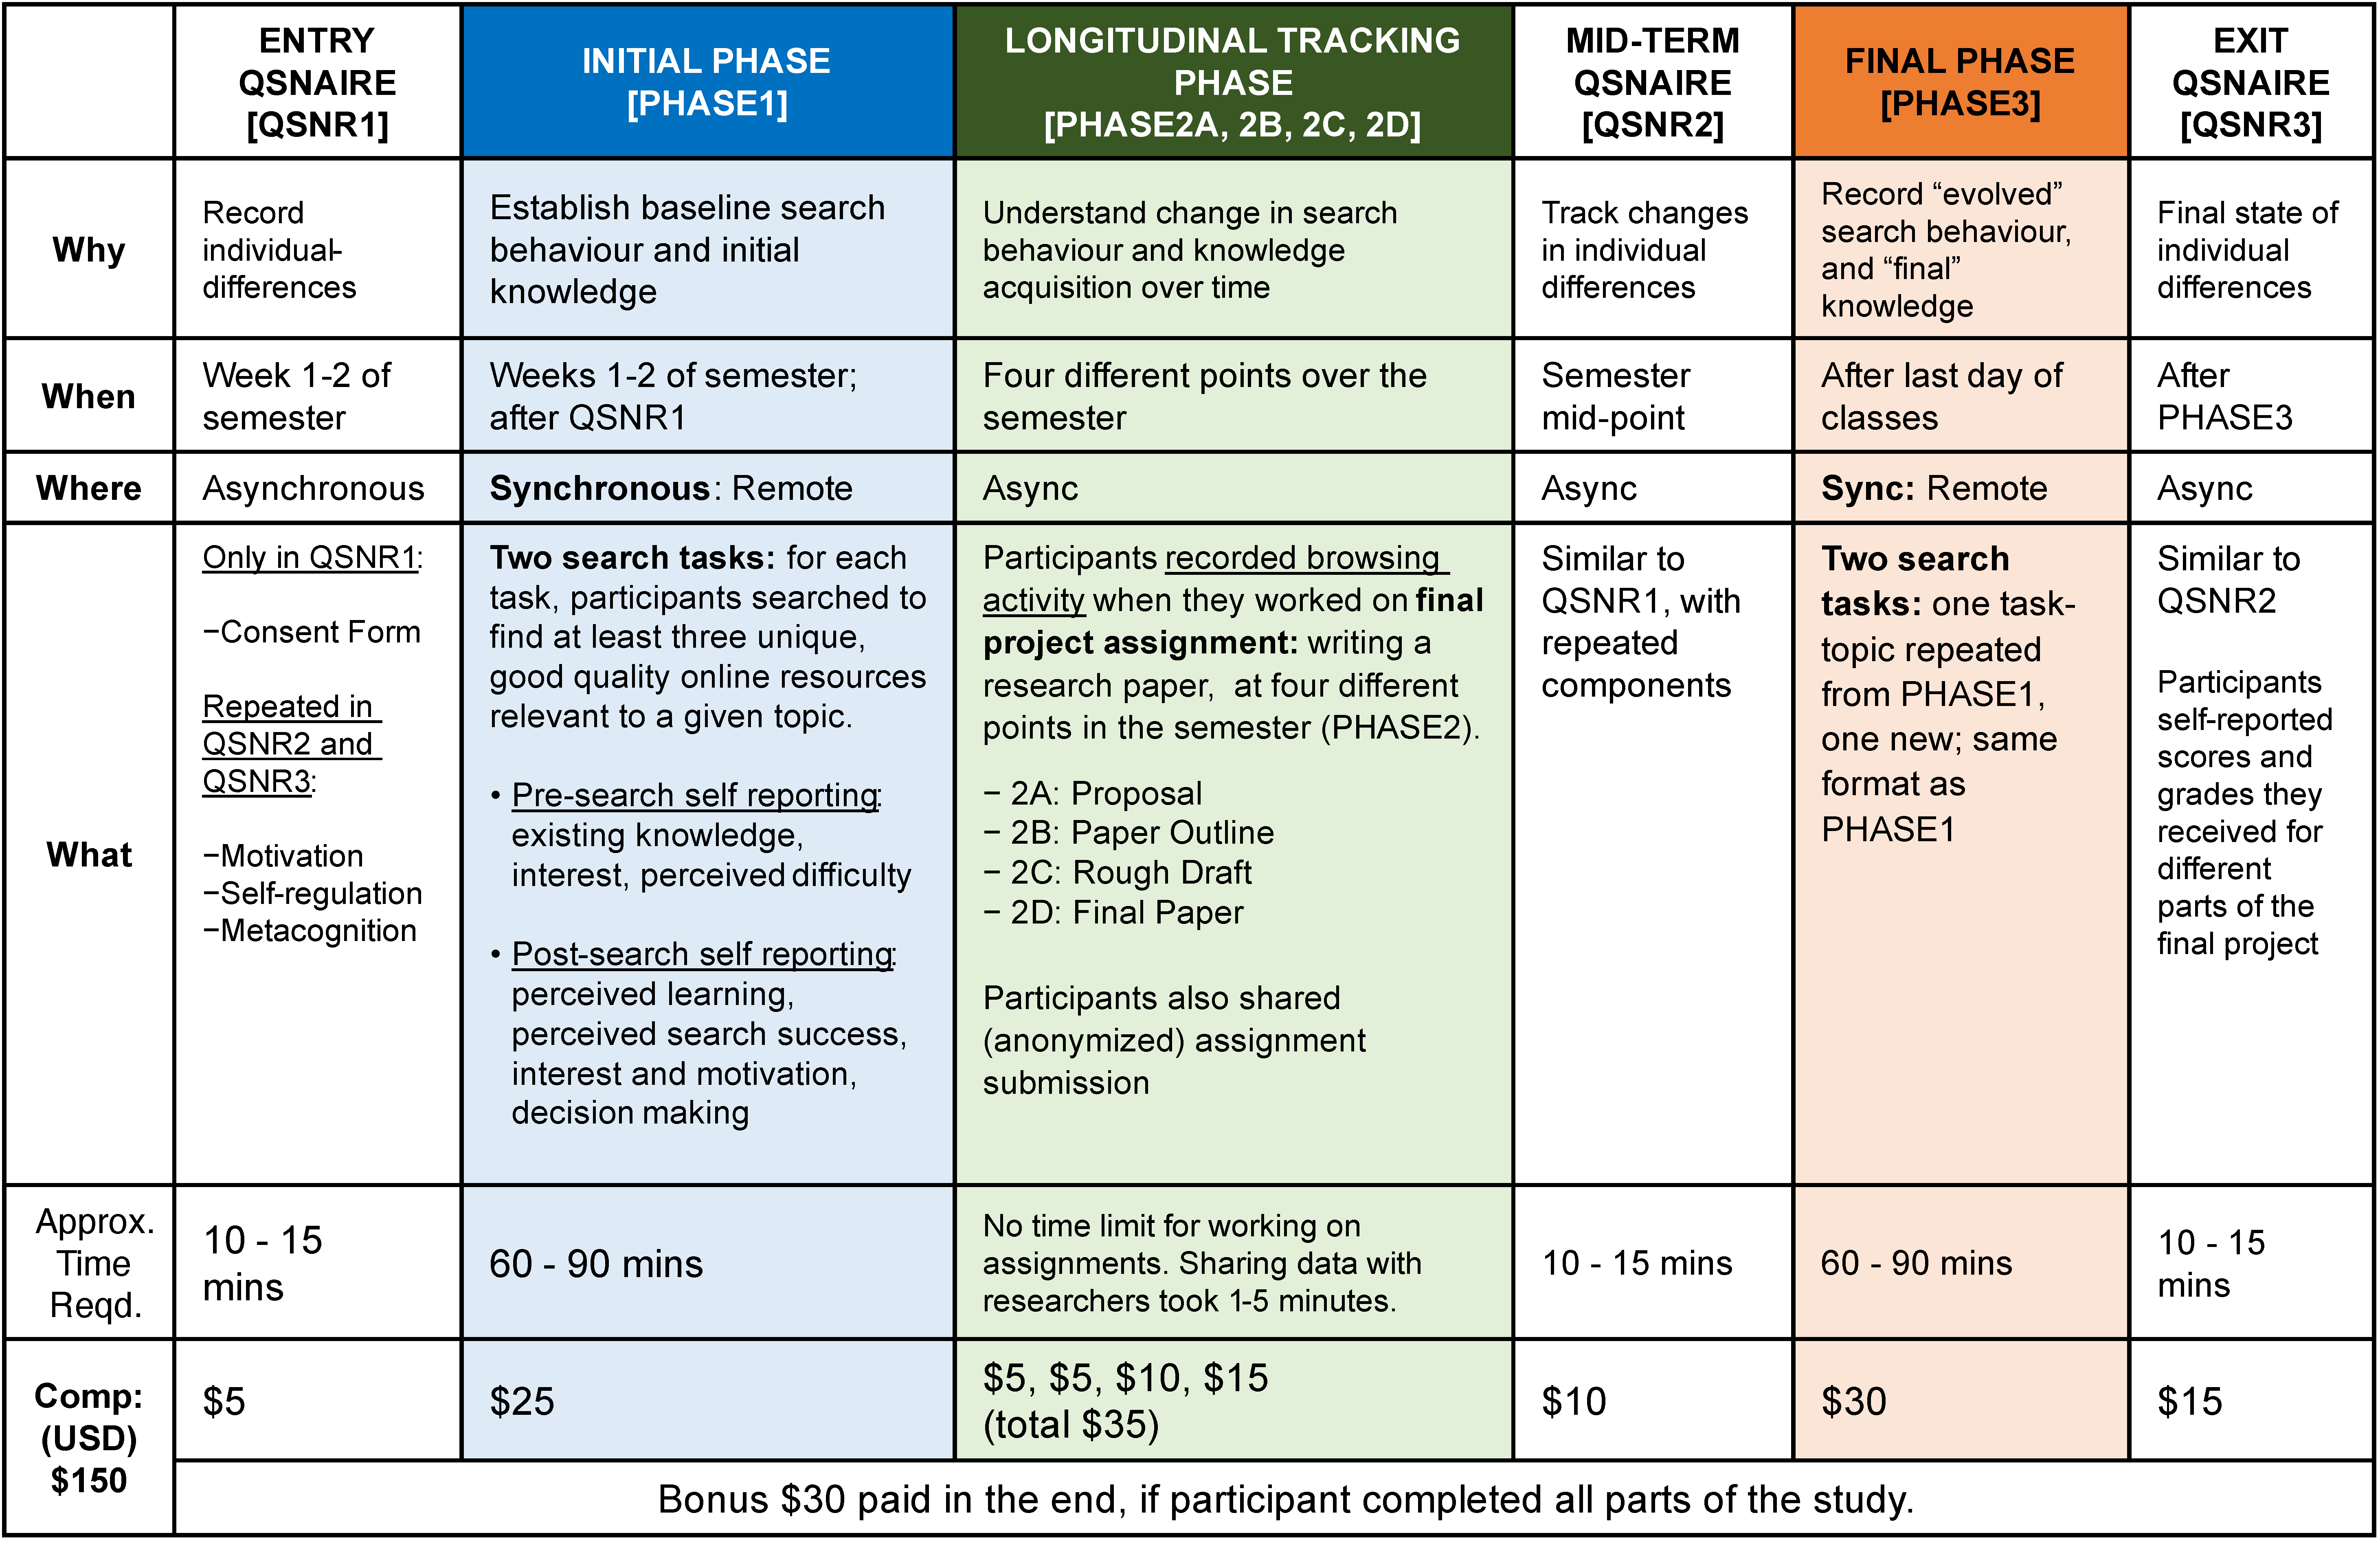
\includegraphics[width=1\linewidth]{figs/study-proc} 

}

\caption[Longitudinal study procedure.]{Longitudinal study procedure.}\label{fig:study-proc}
\end{figure}





The longitudinal study consisted of six data collection components, as illustrated in Figure \ref{fig:study-proc}.
They comprise three asynchronous \textbf{questionnaires} (\texttt{QSNR1}, \texttt{QSNR2}, \texttt{QSNR3}),
two \textbf{remote synchronous study phases} over Zoom video conferencing software (\texttt{PHASE1}, \texttt{PHASE3}),
and a set of four asynchronous \textbf{longitudinal tracking phases} (\texttt{PHASE2a}, \texttt{PHASE2b}, \texttt{PHASE2c}, \texttt{PHASE2d}).
These phases are discussed in detail in the following sections.

\hypertarget{sec-method-qsnr0}{%
\subsection{\texorpdfstring{\texttt{QSNR0}: Recruitment Questionnaire (Appendix \ref{app-qsnr0})}{QSNR0: Recruitment Questionnaire (Appendix \ref{app-qsnr0})}}\label{sec-method-qsnr0}}

Participants were recruited for the study via the recruitment questionnaire (\texttt{QSNR0}).
The questionnaire contained questions about demographic information of the participant pool.
The description of the study and the link to the questionnaire was posted in the Canvas Learning Management System used for the I303 course.

\hypertarget{sec-method-qsnr1}{%
\subsection{\texorpdfstring{\texttt{QSNR1}: Entry Questionnaire}{QSNR1: Entry Questionnaire}}\label{sec-method-qsnr1}}

After recruitment, participants completed the entry questionnaire (QSNR1).
The purpose of QSNR1 was to capture their individual-differences, or
moderating variables, at the beginning of the semester.
Details of the data captured in SUR1 are
described below, with references to sections in the Appendix, where the
full-text of the questionnaire can be found.

\hypertarget{consent-form-appendix-refapp-qsnr-consent-form}{%
\subsubsection{Consent Form (Appendix \ref{app-qsnr-consent-form})}\label{consent-form-appendix-refapp-qsnr-consent-form}}

The first page of QSNR1 was online consent form for participating in the study. Participants
were able to proceed with the study once they provided informed consent.

\hypertarget{motivation-appendix-refapp-qsnr-imi}{%
\subsubsection{Motivation (Appendix \ref{app-qsnr-imi})}\label{motivation-appendix-refapp-qsnr-imi}}

Adapted from the \emph{Intrinsic Motivation Inventory (IMI)} by
(\protect\hyperlink{ref-ryan1982control}{Ryan, 1982}), which is a multidimensional measurement device
intended to assess participants' subjective experience related to a
target activity (the assignments for the course they are taking).
The instrument assesses participants' interest/enjoyment, perceived
competence, effort/importance, pressure/tension, perceived choice,
and value/usefulness, while performing a given activity, thus
yielding six subscale scores.
The pressure/tension and the perceived
choice components were not included in the entry questionnaire QSNR1, and were
present in the mid-term (QSNR2) and exit (QSNR3) questionnaires.

\hypertarget{self-regulation-appendix-refapp-qsnr-srq}{%
\subsubsection{Self-regulation (Appendix \ref{app-qsnr-srq})}\label{self-regulation-appendix-refapp-qsnr-srq}}

Adapted from the \emph{Self-Regulation Questionnaire (SRQ)} by
(\protect\hyperlink{ref-brown1999self}{J. M. Brown et al., 1999}), which assess seven self-regulatory processes
through self-report: receiving relevant information, evaluating the
information and comparing it to norms, triggering change, searching
for options, formulating a plan, implementing the plan, and
assessing the plan's effectiveness (Section \ref{sec-bg-learn-self-regulation}).

\hypertarget{metacognition-appendix-refapp-qsnr-mai}{%
\subsubsection{Metacognition (Appendix \ref{app-qsnr-mai})}\label{metacognition-appendix-refapp-qsnr-mai}}

Adapted from the \emph{Metacognivite Awareness Inventory (MAI)},
originally proposed by (\protect\hyperlink{ref-schraw1994assessing}{Schraw \& Dennison, 1994}) as a 52-item true /
false questionnaire, and later revised by (\protect\hyperlink{ref-terlecki2018call}{Terlecki \& McMahon, 2018}) to use
five-point Likert scales. The instrument measures two components of
cognition through self-report: knowledge about cognition, and
regulation of cognition (Section \ref{sec-bg-learn-metacognition}).

After completing QSNR1 offline, participants were instructed to prepare
for the initial synchronous phase, \texttt{PHASE1}, by
installing Firefox web browser and the YASBIL extension on their machines.
This was a one-time step.
If a
participant could not find the time for this step, they were informed
that an extra 5-10 minutes would be taken in the beginning of \texttt{PHASE1} to
complete this step.

The entry questionnaire and the software installation took about
10-15 minutes to complete. Participants were compensated with USD 5
for their time for completing this step. The questionnaire was published to the I-303 course students in
the first week of the Spring 2022 semester.

\hypertarget{sec-method-phase1}{%
\subsection{\texorpdfstring{\texttt{PHASE1}: Initial Phase}{PHASE1: Initial Phase}}\label{sec-method-phase1}}

The \texttt{PHASE1} of the data collection took place in the beginning of the semester.
The data-collection took place over a Zoom video call combined with YASBIL browsing logger installed in the participants' machines.
Participants were asked to share their screen for the whole duration of the phase.
Their screens and audio were recorded for the entire duration.
They had the freedom to turn off their video.
The total time for \texttt{PHASE1} was expected to not exceed 1.5 hours (90 minutes).
Participants were compensated with USD 25 for this phase.
The different components of \texttt{PHASE1} are described below.

\hypertarget{training-search-task}{%
\subsubsection{Training Search Task}\label{training-search-task}}

Participants performed a training search task to familiarize themselves with how to operate the YASBIL browser extension to log their browsing activity. The training task took around 2-5 minutes.

\hypertarget{phase1-finance-and-phase1-ubuntu-two-actual-search-tasks}{%
\subsubsection{\texorpdfstring{\texttt{PHASE1-FINANCE} and \texttt{PHASE1-UBUNTU}: Two Actual Search Tasks}{PHASE1-FINANCE and PHASE1-UBUNTU: Two Actual Search Tasks}}\label{phase1-finance-and-phase1-ubuntu-two-actual-search-tasks}}

\begin{figure}

{\centering 
\includegraphics[width=1\linewidth]{figs/search-task-repeated} 

}

\caption[Prompts for repeated search task.]{Prompts for the search task that was repeated in the final phase, on the topic of financial literacy.}\label{fig:search-task-repeated}
\end{figure}





Participants performed two search tasks: \texttt{PHASE1-FINANCE}, and \texttt{PHASE1-UBUNTU}.
The \texttt{PHASE1-FINANCE} task was repeated at the end of the semester as \texttt{PHASE3-FINANCE} task.
The \texttt{PHASE1-UBUNTU} task was not repeated, and instead the \texttt{PHASE3-BIAS} task tooK its place.
This helps to answer the research question RQ2 (Chapter \ref{ch-rq}).
The order of the two search tasks were randomized.

The repeated search task \texttt{FINANCE} was on the topic of financial literacy, a topic that we posit can be considered as universally important to college students, and part of lifelong learning.
The prompts for the \texttt{PHASE1-FINANCE} and \texttt{PHASE3-FINANCE} tasks are presented in Figure \ref{fig:search-task-repeated}.
The non-repeated search tasks were on topics that were taught in the I303 course:
Ubuntu ethics (for \texttt{PHASE1})
and
Algorithmic Bias (for \texttt{PHASE3}).
The prompts for these tasks are present in Figure \ref{fig:search-task-new}.

\begin{figure}

{\centering 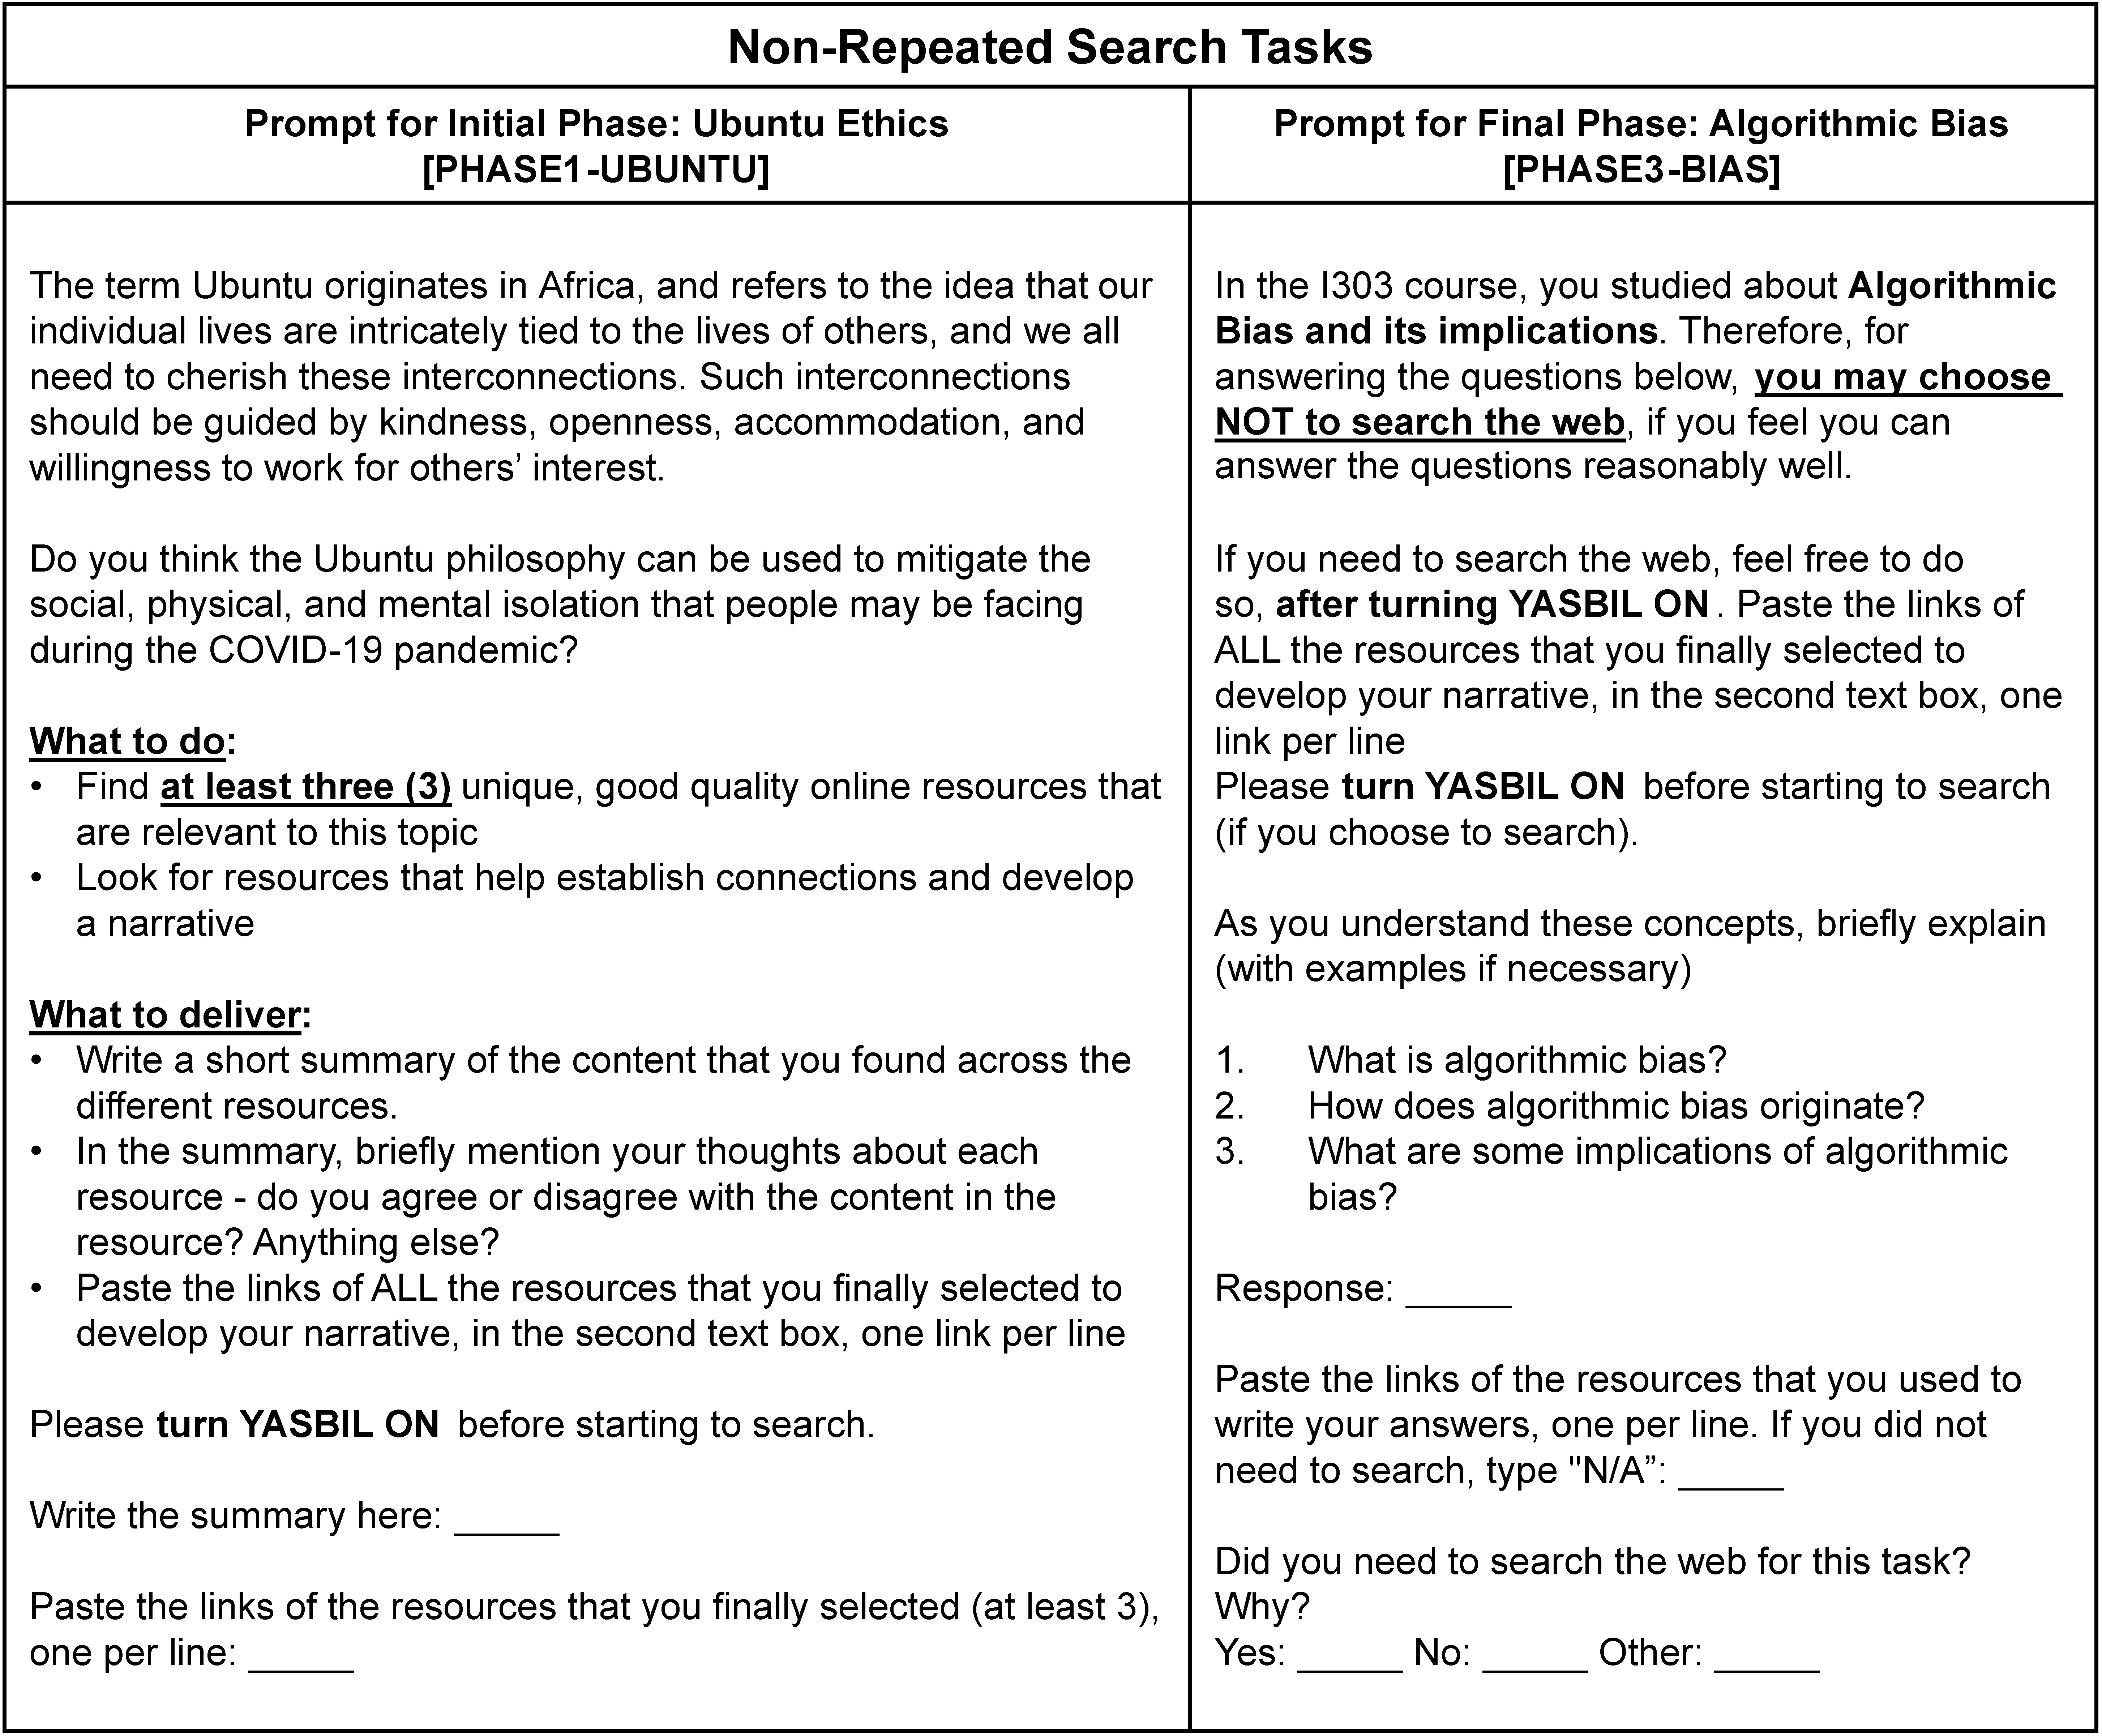
\includegraphics[width=1\linewidth]{figs/search-task-new} 

}

\caption[Prompts for non-repeated search task.]{Prompts for the non-repeating search tasks. Topics were selected from the I-303 course content.}\label{fig:search-task-new}
\end{figure}





Each search task began with a pre-task questionnaire (Appendix \ref{app-phase13-pretask}), which asked participants to self-rate their pre-search knowledge-level and interest on the topic.
Then participants turned on the YASBIL browsing logger and started searching.
The deliverable for each search task was a written summary (artefact).
After participants are satisfied with the quality of the deliverable, they turned off YASBIL browsing logger, and proceeded to the post-task questionnaire.

The post-task questionnaire (Appendix \ref{app-phase13-posttask}) asked participants to self-rate their perceived learning and search outcomes, search experience, interest and motivation, and overall perceptions.
The pre-task and post-task questionnaires are adapted from (\protect\hyperlink{ref-collins2016assessing}{Collins-Thompson et al., 2016}; \protect\hyperlink{ref-crescenzi2020adaptation}{Crescenzi, 2020}).

\hypertarget{memory-span-test}{%
\subsubsection{Memory Span Test}\label{memory-span-test}}

\texttt{PHASE1} concluded with the assessment of the participant's working memory capacity (WMC) using a memory span task (\protect\hyperlink{ref-francis2004coglab}{Francis et al., 2004}).
Memory span assessment was kept in the synchronous phase because it is a timed task, and needs to conducted in a controlled (experimenter observed) condition.
The task has 25 trials. On each trial participants saw a list of items presented one at a time in random order and were asked to recall the items in the same order in which they were presented. If they got a list correct, the list length increased by 1 for that type of material. If they got a list incorrect, the list length decreased by 1.

The type of material participants were asked to recall were: digits, letters that sound dissimilar, letters that sound similar, short words, and long words. The outcome score was the list length of the last list that participants could correctly recall.

\hypertarget{sec-method-phase2}{%
\subsection{\texorpdfstring{\texttt{PHASE2A} - \texttt{PHASE2D}: Longitudinal Tracking Phase}{PHASE2A - PHASE2D: Longitudinal Tracking Phase}}\label{sec-method-phase2}}

\begin{figure}

{\centering 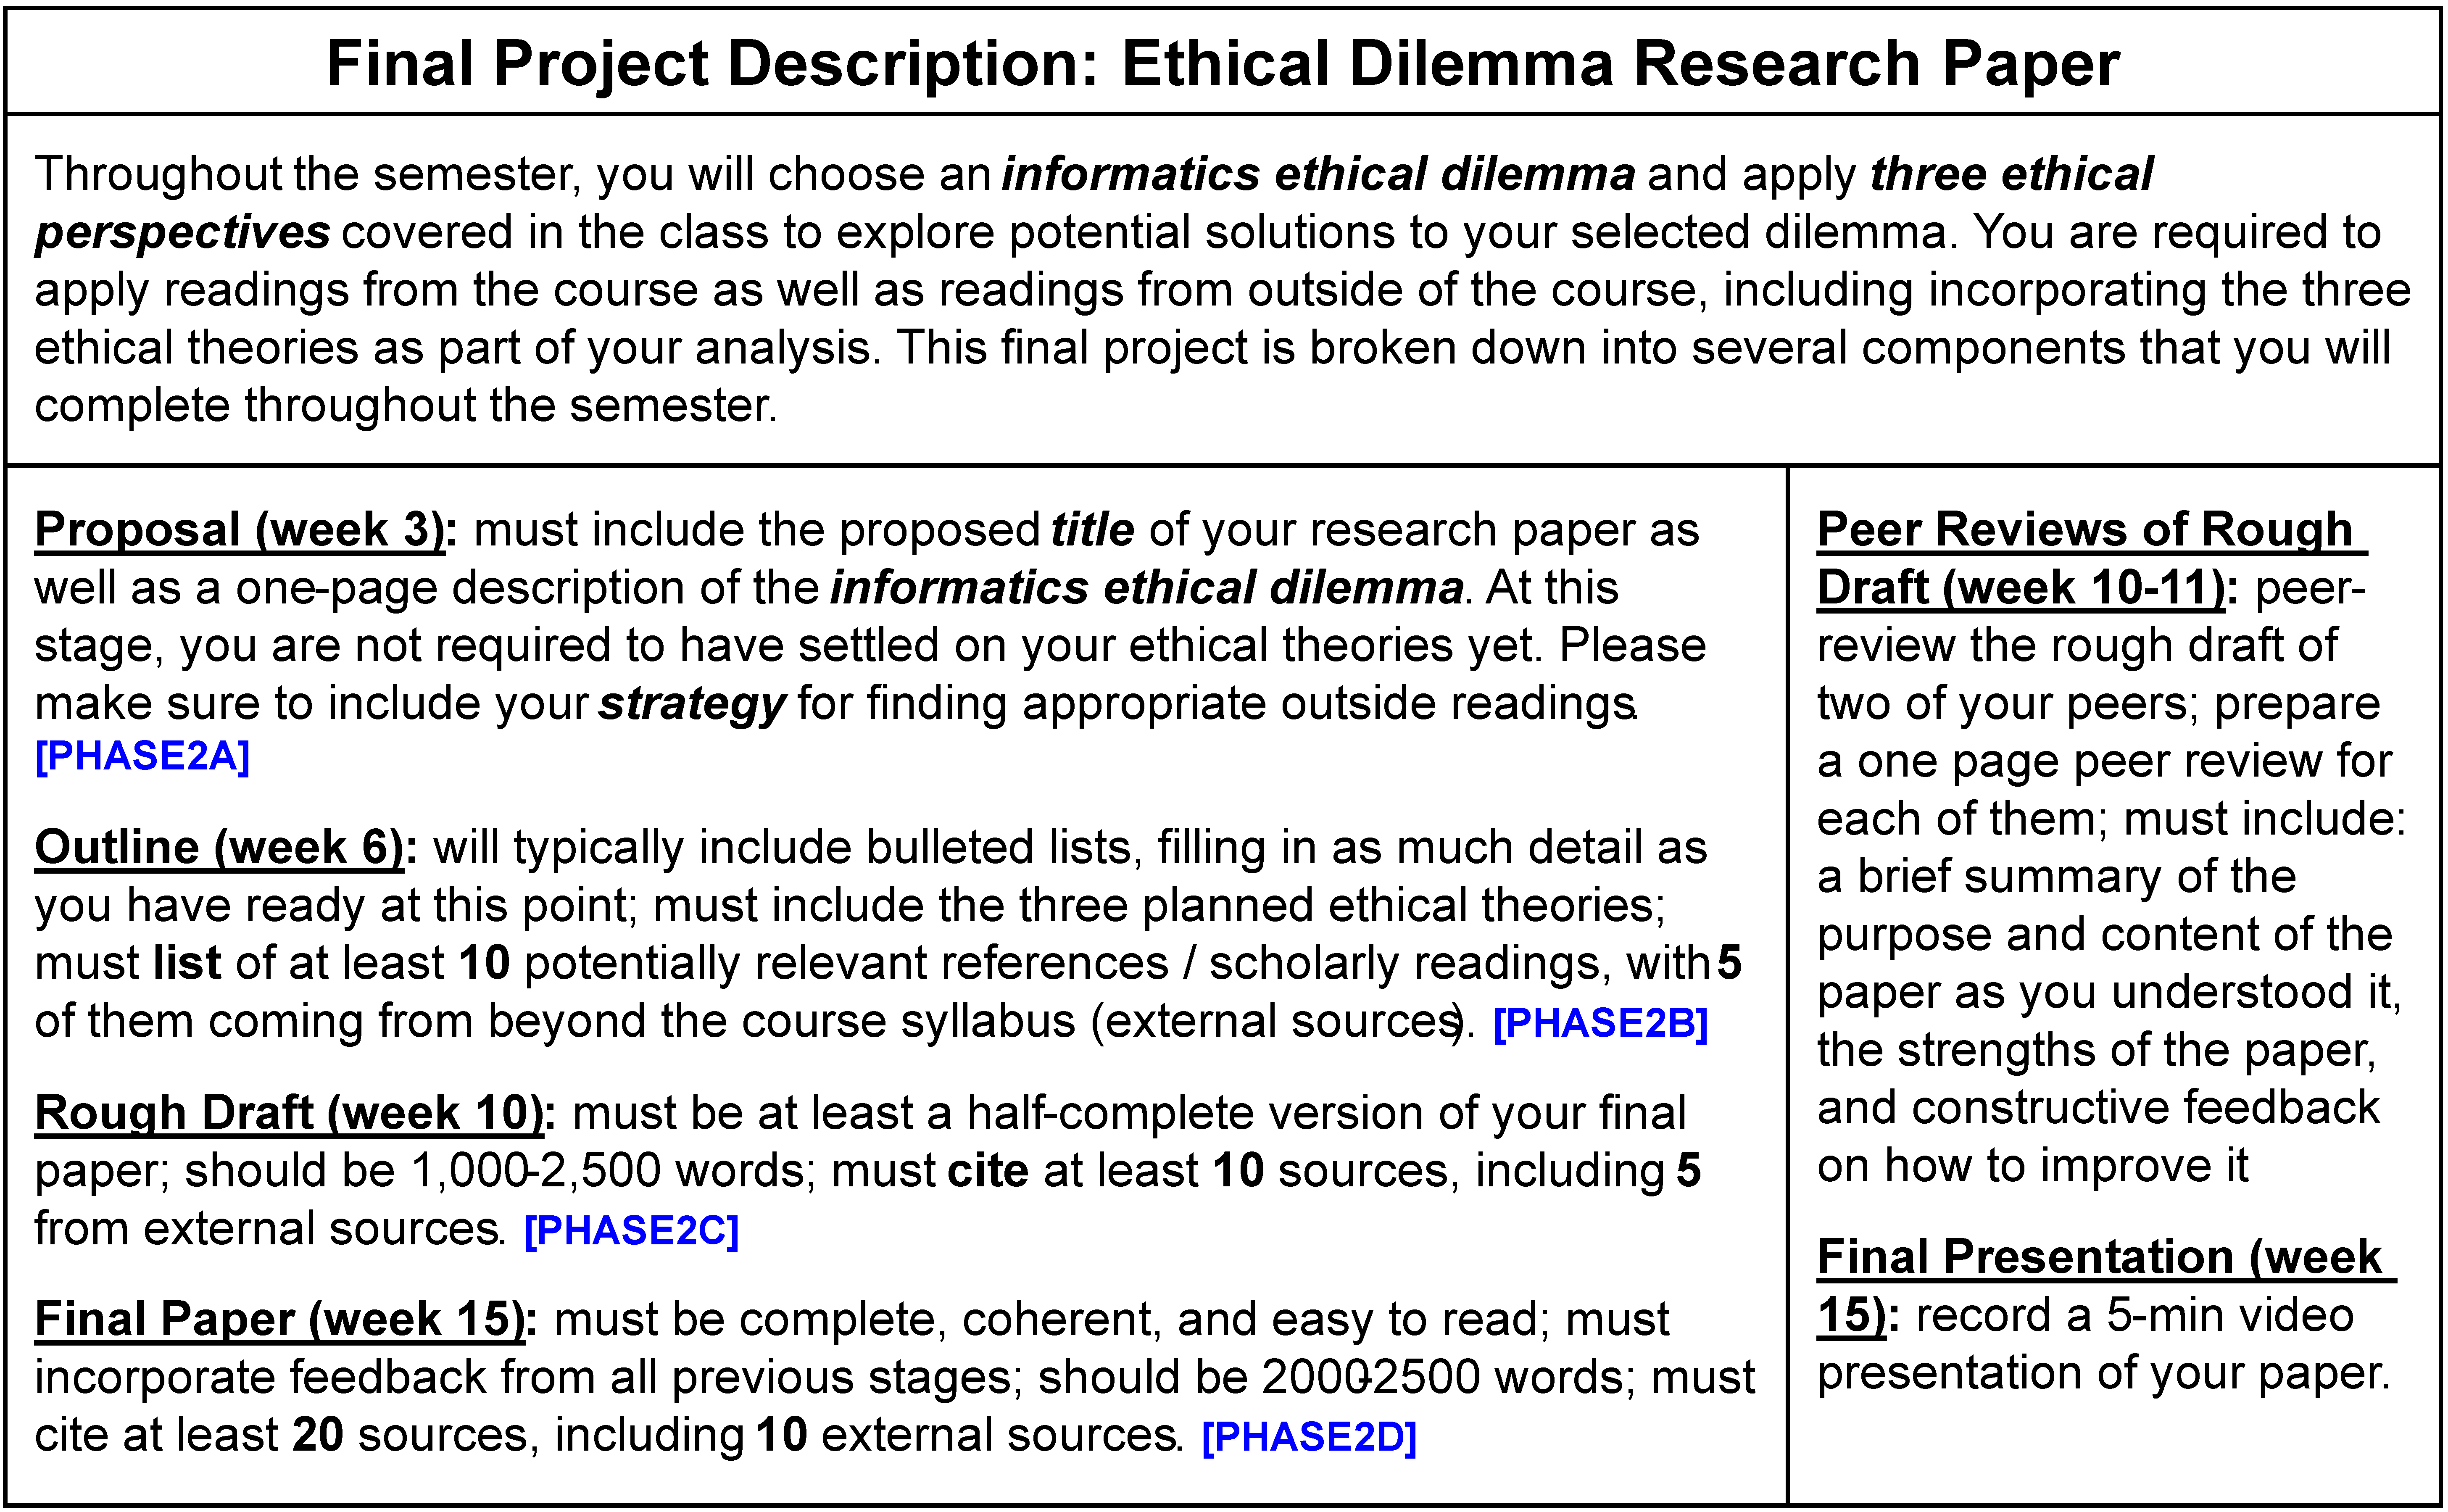
\includegraphics[width=1\linewidth]{figs/final-project-description} 

}

\caption[Final project description.]{Final project description, setting up the longitudinal tracking phase of the study throughout the duration of the Spring 2022 semester. Text taken from I-303 course syllabus (\protect\hyperlink{ref-fleischmann2022i303}{Fleischmann et al., 2022}); emphasis and annotations our own.}\label{fig:final-project-description}
\end{figure}





The four-part longitudinal tracking phases \texttt{PHASE2A} - \texttt{PHASE2D} were conducted asynchronously over the duration of the semester, to understand the change (or lack thereof) of participants' search behaviour and knowledge gain over time.
Whenever participants worked on different parts of their final project (Ethical dilemma research paper for the I-303 course), as described in Figure \ref{fig:final-project-description}, they used Firefox web browser, and logged their browsing activity using YASBIL browsing logger.
To protect their privacy, participants were regularly instructed to turn YASBIL on only when they were searching for information related to coursework.
After each checkpoint assignment, participants self-uploaded an anonymized version of the working-draft of their research paper, and answered a post-task questionnaire.
The post-task questionnaire were similar to those used in the \texttt{PHASE1} and \texttt{PHASE3} search tasks, where participants self-reported, among other things, their perceived learning outcome and perceived search outcome (\protect\hyperlink{ref-collins2016assessing}{Collins-Thompson et al., 2016}).
Participants received reminder emails before the deadline of each assignment, to remind them to use Firefox, turn YASBIL on, and upload the anonymized working-draft.
To prevent participant drop-off, a staggered payment model was adopted during PHASE2.
Participants received USD 5 each when they completed \texttt{PHASE2A} and \texttt{PHASE2B}, USD 10 for \texttt{PHASE2C}, and USD 15 for \texttt{PHASE2D}, for a total of USD 35 for entire \texttt{PHASE2}.

\hypertarget{sec-method-qsnr2}{%
\subsection{\texorpdfstring{\texttt{QSNR2}: Mid-Term Questionnaire}{QSNR2: Mid-Term Questionnaire}}\label{sec-method-qsnr2}}

The mid-term questionnaire \texttt{QSNR2} took place around the mid-point of the semester (Week 8-9).
The purpose was to track whether any of the participants' individual difference measures (motivation, metacognition, and self-regulation) changed during the first half of the semester.
This questionnaire was essentially a replica of the Entry Questionnaire \texttt{QSNR1}, with two modifications. First, the consent form and the demographics sections were absent.
Second, the Intrinsic Motivation Inventory (IMI) included the `pressure/tension' and the `perceived choice' subscales, as these scales are more meaningful after an activity has taken place (\protect\hyperlink{ref-ryan1982control}{Ryan, 1982}).
The IMI was also be reworded to reflect the mid-point of the semester.
Participants were compensated with USD 10 for completing this step.

\hypertarget{sec-method-phase3}{%
\subsection{\texorpdfstring{\texttt{PHASE3}: Final Phase}{PHASE3: Final Phase}}\label{sec-method-phase3}}

The Final Phase \texttt{PHASE3} was similar in structure to the Initial Phase (\texttt{PHASE1}), and took place at the end of the semester, after all the course related tasks were completed by the participant. The purpose of the session is to record the `evolved' search behaviour, and final knowledge state.
Participants performed two search tasks: \texttt{PHASE3-FINANCE} and \texttt{PHASE3-BIAS}.

At the end of \texttt{PHASE3}, a semi-structured interview was conducted.
The questions were aimed to collect the participants' reflections on their searching and learning experience throughout the semester, w.r.t. to the I303 course.
While a full-scale qualitative analysis of the interview responses is beyond the scope of this dissertation, some preliminary qualitative quotes are presented in the results and discussion sections, to support the quantitative results as necessary.

\hypertarget{phase3-finance-and-phase3-bias-two-actual-search-tasks}{%
\subsubsection{\texorpdfstring{\texttt{PHASE3-FINANCE} and \texttt{PHASE3-BIAS}: Two Actual Search Tasks}{PHASE3-FINANCE and PHASE3-BIAS: Two Actual Search Tasks}}\label{phase3-finance-and-phase3-bias-two-actual-search-tasks}}

Of the two search tasks, the topic of one was repeated from \texttt{PHASE1} (financial literacy, Figure \ref{fig:search-task-repeated}), while the topic of the other came from the course material: algorithmic bias (Figure \ref{fig:search-task-new}).
In both search tasks, participants were given the option of \textbf{\emph{not searching}} if they felt confident enough to answer the search task questions from their prior knowledge (\protect\hyperlink{ref-crescenzi2020adaptation}{Crescenzi, 2020}).
The deliverables for each search-task, as before, was a written summary (artefact).

Similar to \texttt{PHASE1}, participants were asked to share their screen for the whole duration of the phase.
Their screen and audio was recorded for the same. They had the freedom to turn off their video. The total time for \texttt{PHASE3} was expected to not exceed 1.5 hours (90 minutes).
Participants were compensated with USD 30 for \texttt{PHASE3}.
At the end of \texttt{PHASE3}, participants were instructed to complete the Exit Questionnaire \texttt{QSNR3} as soon as convenient.

\hypertarget{sec-method-qsnr3}{%
\subsection{\texorpdfstring{\texttt{QSNR3}: Exit Questionnaire}{QSNR3: Exit Questionnaire}}\label{sec-method-qsnr3}}

The exit questionnaire \texttt{QSNR3} took place after the Final Phase \texttt{PHASE3}.
The purpose was to record the final state of the participants' individual difference measures (motivation, metacognition, self-regulation), and whether these characteristics changed during the second half of the semester.
As before, \texttt{QSNR3} questionnaire was essentially be a replica of \texttt{QSNR2}, with the Intrinsic Motivation Inventory (IMI) reworded to reflect the end-point of the semester
Participants were be compensated with USD 15 for their time for completing this step.

After \texttt{QSNR3} was complete, participants received a bonus compensation of USD 30, if they completed all the phases of the LongSAL study without missing anything.

\hypertarget{measures-to-address-ethical-concerns}{%
\section{Measures to Address Ethical Concerns}\label{measures-to-address-ethical-concerns}}

\begin{itemize}
\item
  Participation in the study (which was voluntary and compensated separately) and participation in the I303 course (which was required for graduation from the Informatics major) were sufficiently disentangled. The course instructors were never aware of which students participate in the course, and did not share any student data with the researchers. This avoided any undue pressure or expectation on the students.
\item
  Participants logged their browsing activity using a Firefox browser extension YASBIL, which was been developed by the authors. The extension has an ON-OFF button, which put the participants in full control of when they wished to start and stop the logging. Participants had been sufficiently trained to use the browser extension, and were repeatedly reminded to log data only when they were working on the research paper assignments for the course, and not at other times.
\item
  This study has been approved by The University of Texas at Austin Institutional Review Board (Submission ID: STUDY00002136, Date Approved: December 8, 2021).
\end{itemize}

After data collection for all the phases was complete, data analysis was performed on the collected data, which is discussed in the next chapter.

\hypertarget{data-analysis-results-and-discussion-longitudinal-tracking-phase}{%
\chapter{Data Analysis, Results, and Discussion: Longitudinal Tracking Phase}\label{data-analysis-results-and-discussion-longitudinal-tracking-phase}}

The longitudinal phase of the LongSAL study involved understanding students' searching as learning behaviour for the research paper writing task. The aim was to investigate how students' information search behaviours and learning outcomes change over time.
This chapter presents participant information, the timeline of data collection, and data analysis steps, followed by the results of the longitudinal phase of the study.
The findings from the initial and final phases are presented in the next chapter for better narration.

\hypertarget{participants-and-timeline-of-collected-data}{%
\section{Participants and Timeline of Collected Data}\label{participants-and-timeline-of-collected-data}}

\begin{figure}

{\centering 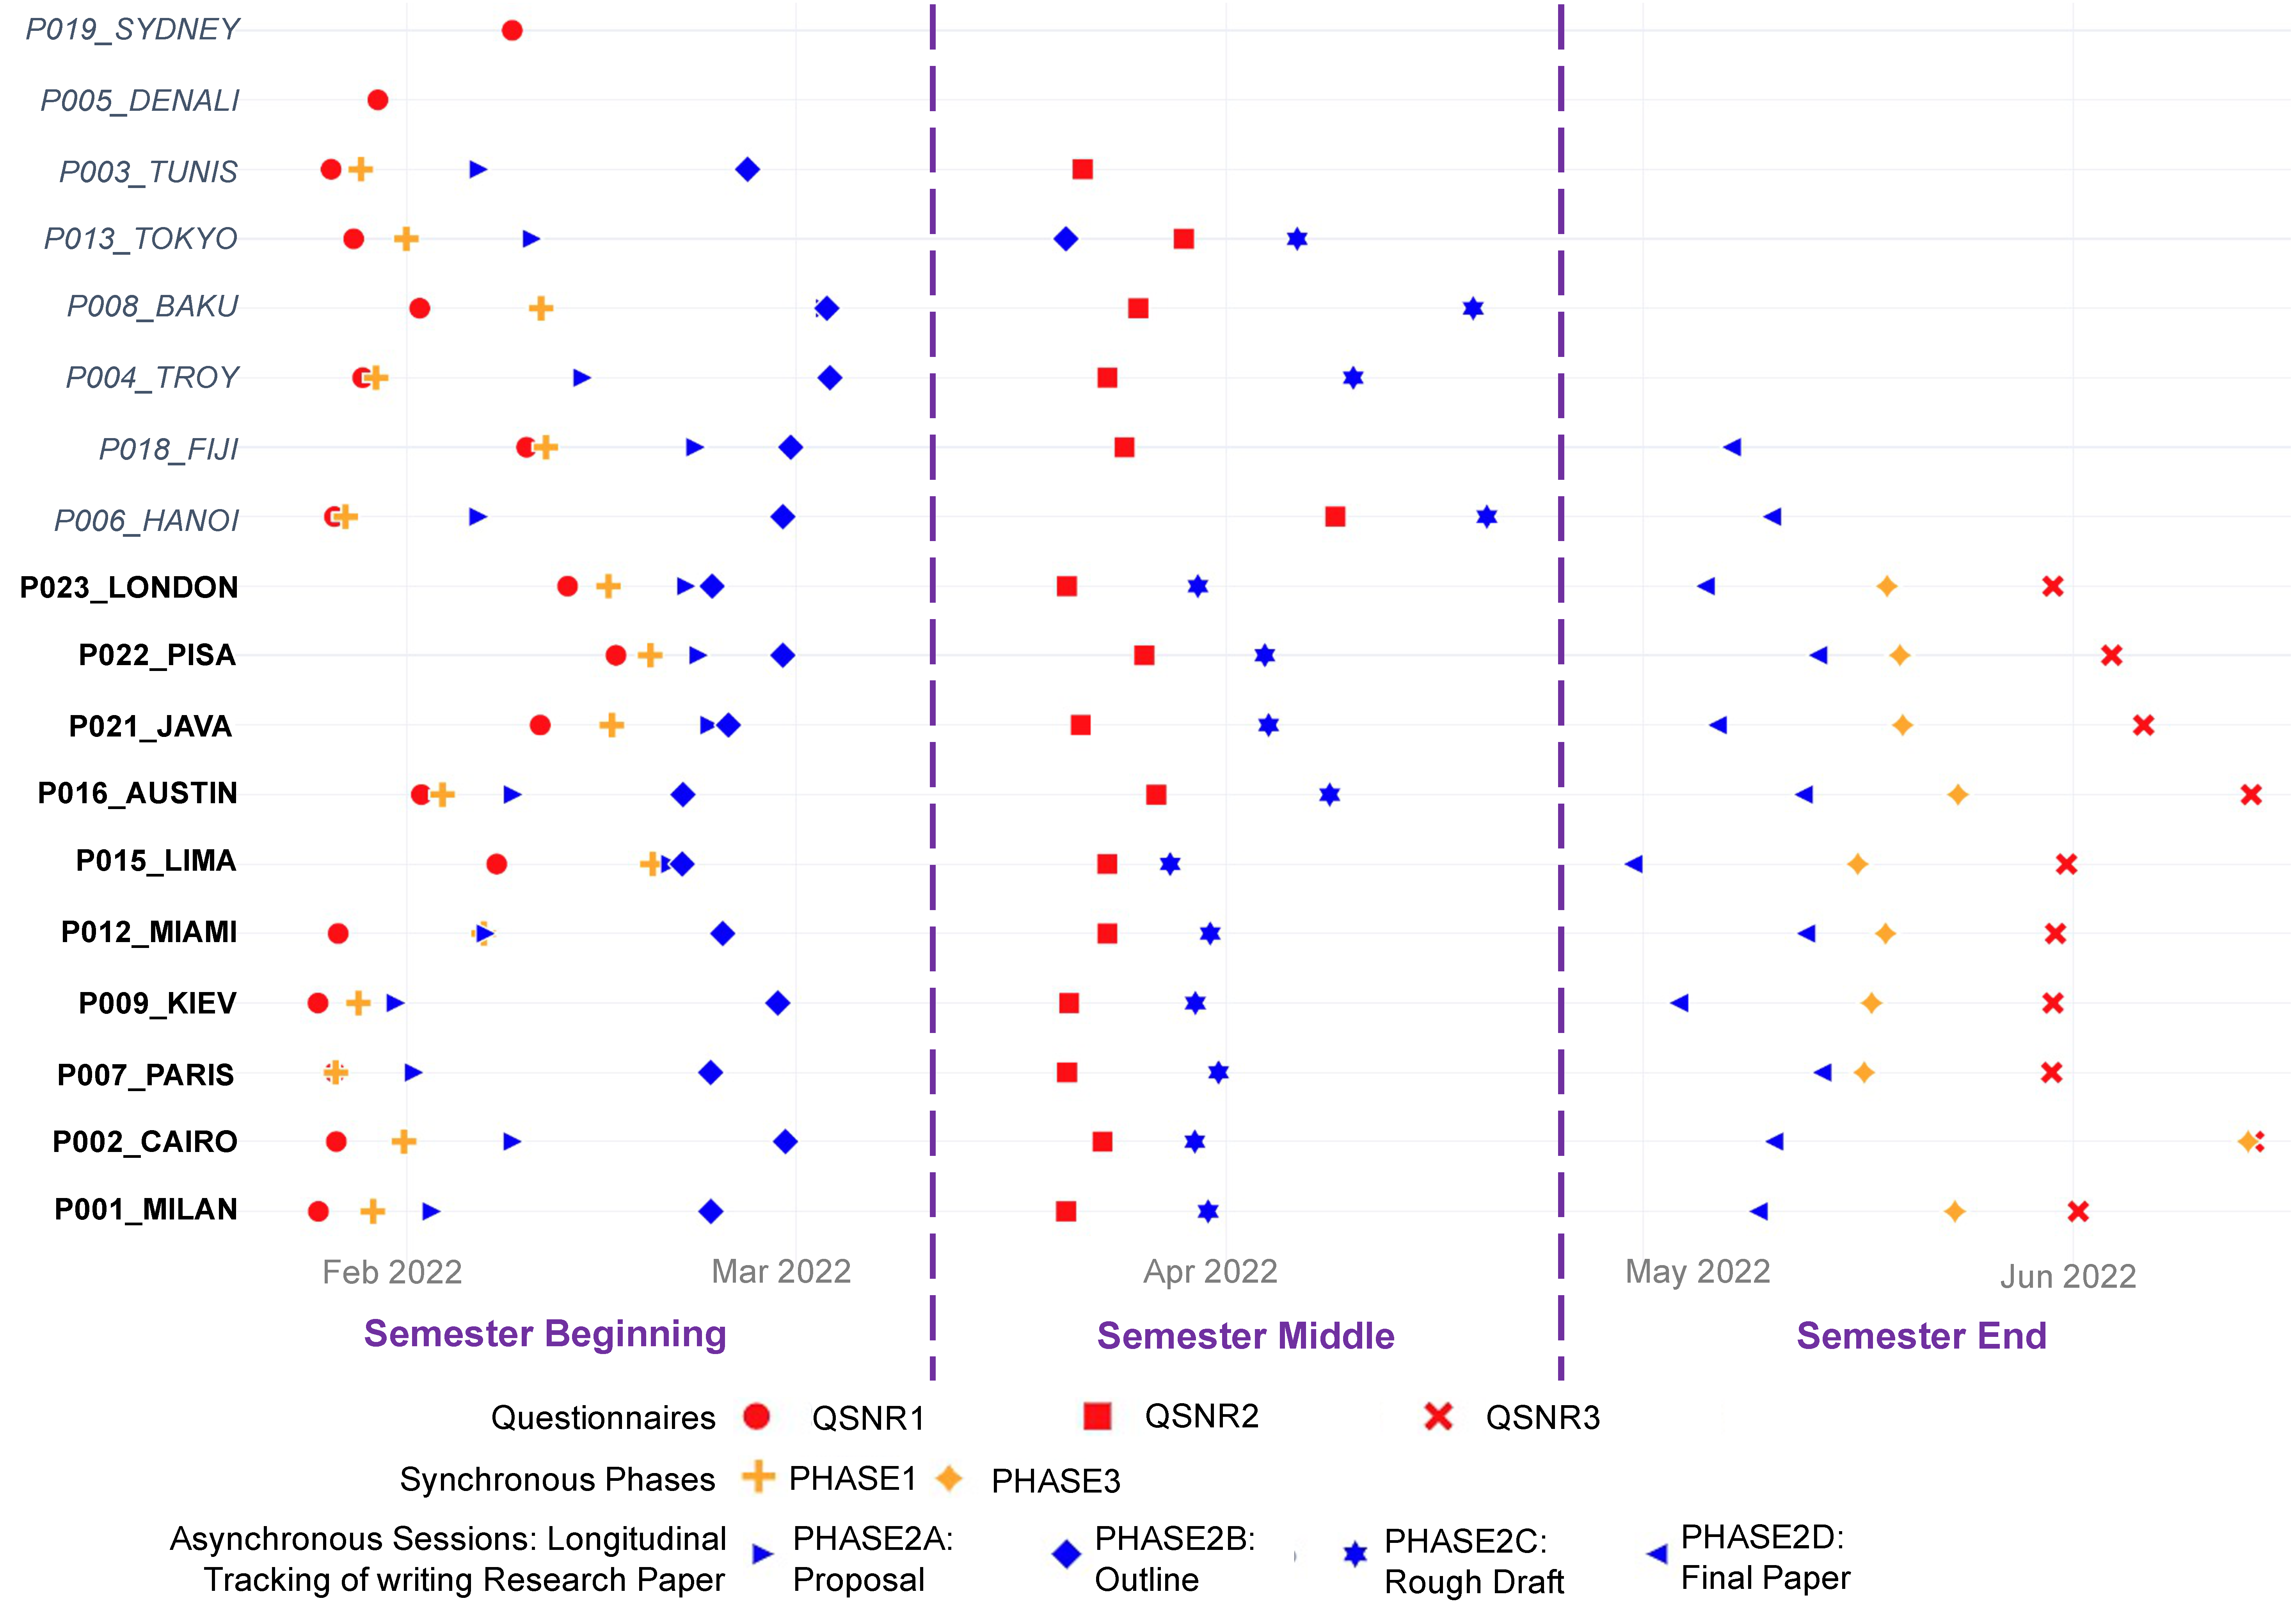
\includegraphics[width=1\linewidth]{figs/res-timeline-collected-data} 

}

\caption[Timeline of collected data.]{Timeline of collected data.}\label{fig:res-timeline-collected-data}
\end{figure}





Figure \ref{fig:res-timeline-collected-data} shows the timeline of the data collected in the LongSAL study, spread across the Spring 2022 semester at the University of Texas at Austin, USA.
Eighteen participants enlisted their names in the Recruitment Questionnaire, \texttt{QSNR0}.
Sixteen showed up for the initial phase and remained in the study till the mid-point of the semester (mid-term questionnaire, \texttt{QSNR2}).
Then six participants dropped off, and ten participants fully completed the study (who stayed until the exit questionnaire, \texttt{QSNR3}.)
In Figure \ref{fig:res-timeline-collected-data}, participant names in \textbf{bold} (bottom 10) indicate those who fully completed the longitudinal study,
while participant names in \emph{italics} (top 8) indicate those who dropped off at various stages along the way.
For data analysis, we partitioned the semester duration into three phases along the green vertical dotted lines: beginning, middle, and end of the semester.
Inspired by the Spanish TV series \emph{La Casa de Papel} (English name: \emph{Money Heist})\footnote{\url{https://en.wikipedia.org/wiki/Money_Heist}}, participants were assigned code-names which were aliases of geographic locations.

\hypertarget{data-analysis-framework}{%
\section{Data Analysis Framework}\label{data-analysis-framework}}

\begin{figure}

{\centering 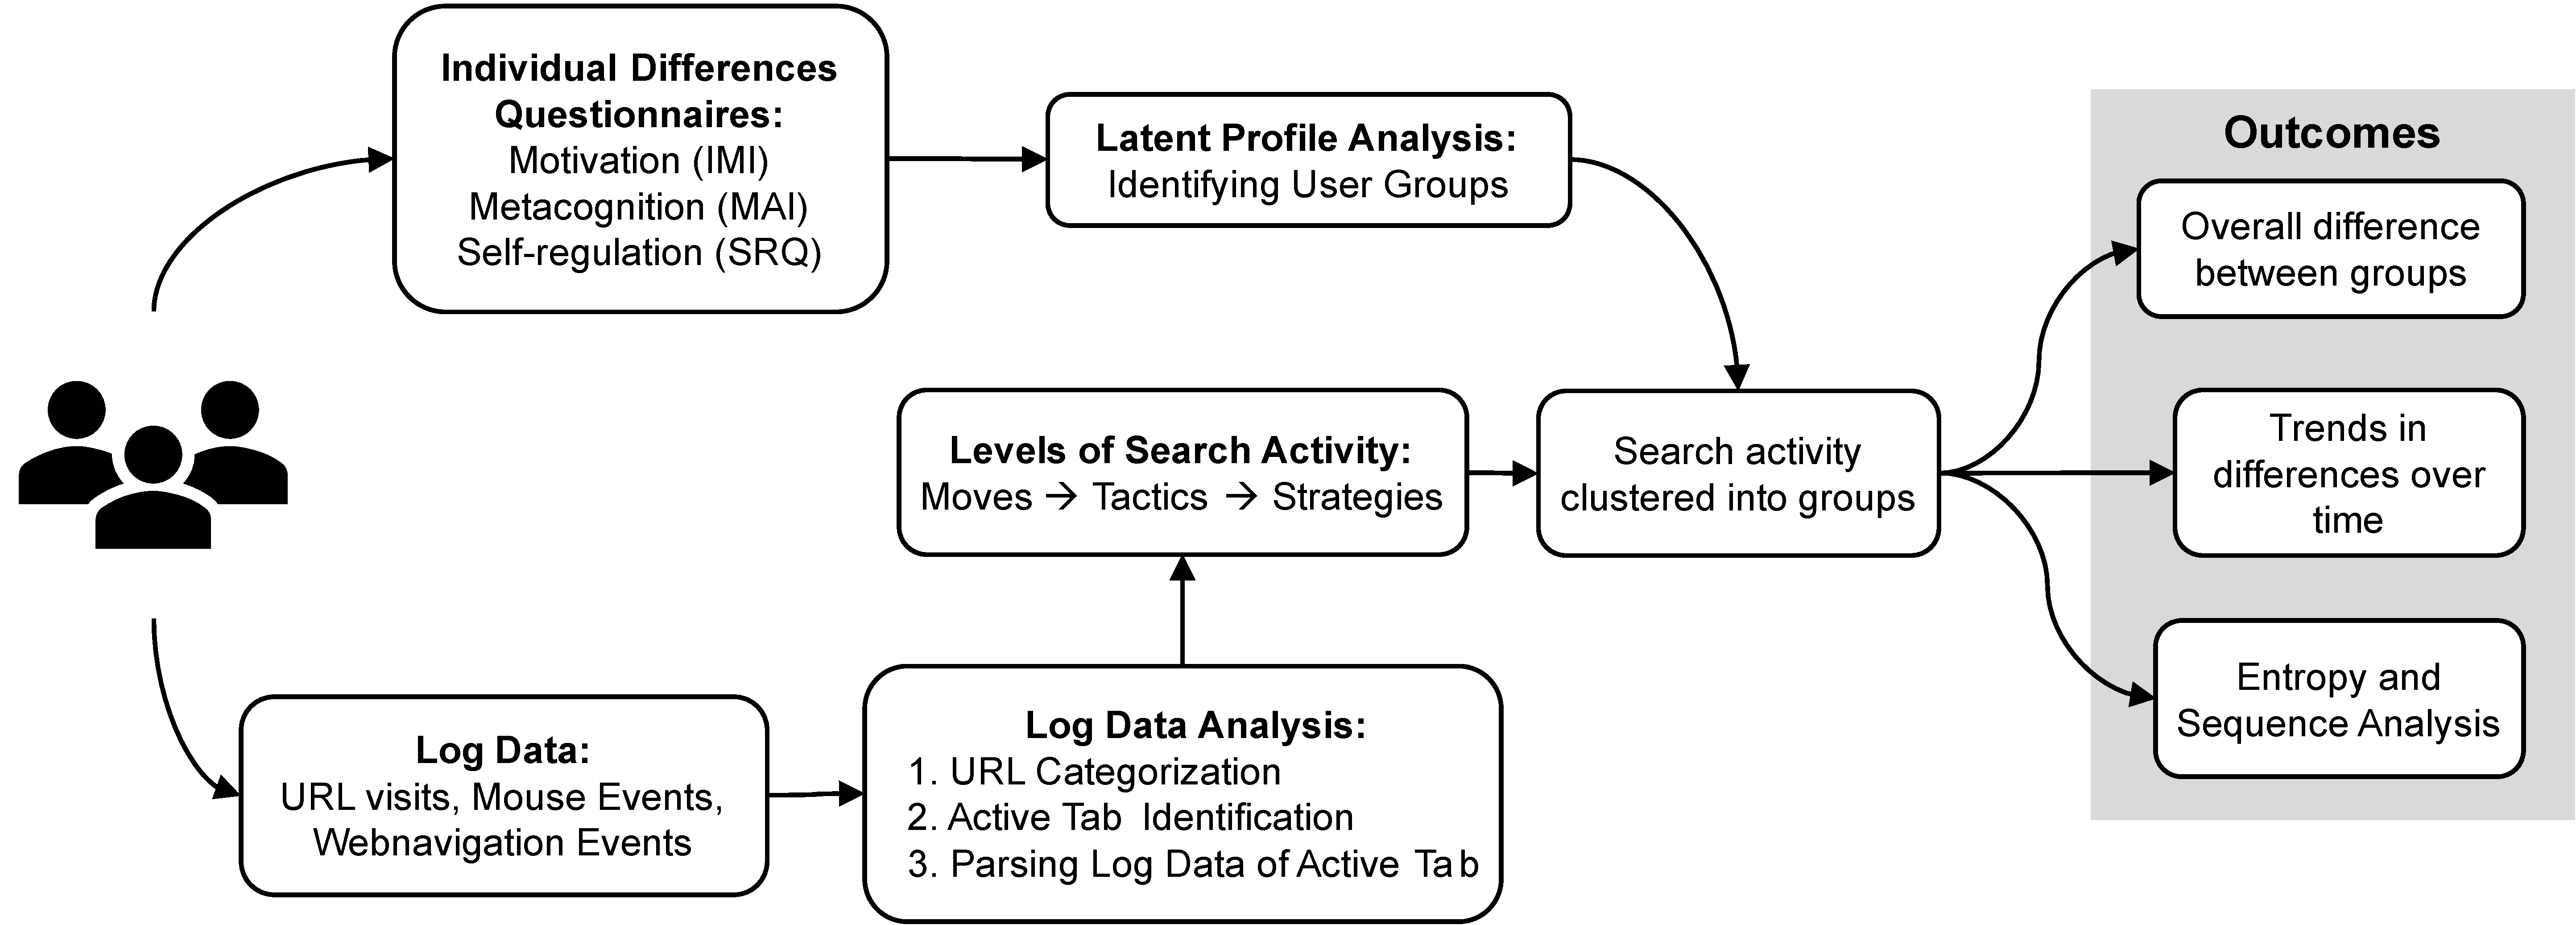
\includegraphics[width=1\linewidth]{figs/data-analysis-framework} 

}

\caption[Data analysis framework.]{Data analysis framework followed in this dissertation.}\label{fig:data-analysis-framework}
\end{figure}





The general framework for analysing the data collected in the \emph{LongSAL} study is described in Figure \ref{fig:data-analysis-framework}.
Primarily, two categories of data were collected in the study:
explicit responses via Qualtrics survey platform, and implicit search behaviours via YASBIL browsing logger.
The data collected from Qualtrics were primarily search task written responses, as well as responses to the individual difference questionnaire instruments for motivation, metacognition, and self-regulation.
Data from the questionnaires were used to divide participants into groups, which is discussed in Section \ref{sec-res-phase2-lpa}.
Log data from YASBIL was cleaned, processed, categorized (Section \ref{sec-res-url-categorization}) and analysed, to examine (differences in) search behaviour of different participant groups.

For examining statistical differences between groups, we employed the non-parametric \textbf{Mann-Whitney U test} for null-hypothesis significance testing (\protect\hyperlink{ref-mann1947test}{Mann \& Whitney, 1947}).
This choice was due to several reasons:
the sample sizes were often small,
the groups were imbalanced, and / or the data did not satisfy the assumptions of parametric tests such as ANOVA.
Employing one statistical test allows for easy comparison between different categories of results.

Additionally, we also report \textbf{Common Language Effect Size (CLES)} for each statistical test result.
The common language effect size is the proportion of pairs where \(x\) from the first group is greater than \(y\) from the second group.
In other words, it is the probability that a score sampled at random from the first distribution will be higher than a score sampled from the second distribution.
CLES was first introduced by McGraw \& Wong (\protect\hyperlink{ref-mcgraw1992common}{1992}).
The Python statistical library employed in the data analysis -- Pingouin (\protect\hyperlink{ref-vallat2018pingouin}{Vallat, 2018}) -- uses a brute-force version of the formula given by Vargha \& Delaney (\protect\hyperlink{ref-vargha2000critique}{2000}).
The advantage is of this method are twofold:
first, the brute-force approach pairs each observation of x to its y counterpart, and therefore does not require normally distributed data;
second, the formula takes ties into account and therefore works with ordinal data \footnote{\url{https://pingouin-stats.org/build/html/generated/pingouin.mwu.html}}.

\hypertarget{sec-res-phase2-lpa}{%
\section{Latent Profile Analysis}\label{sec-res-phase2-lpa}}

\begin{figure}

{\centering 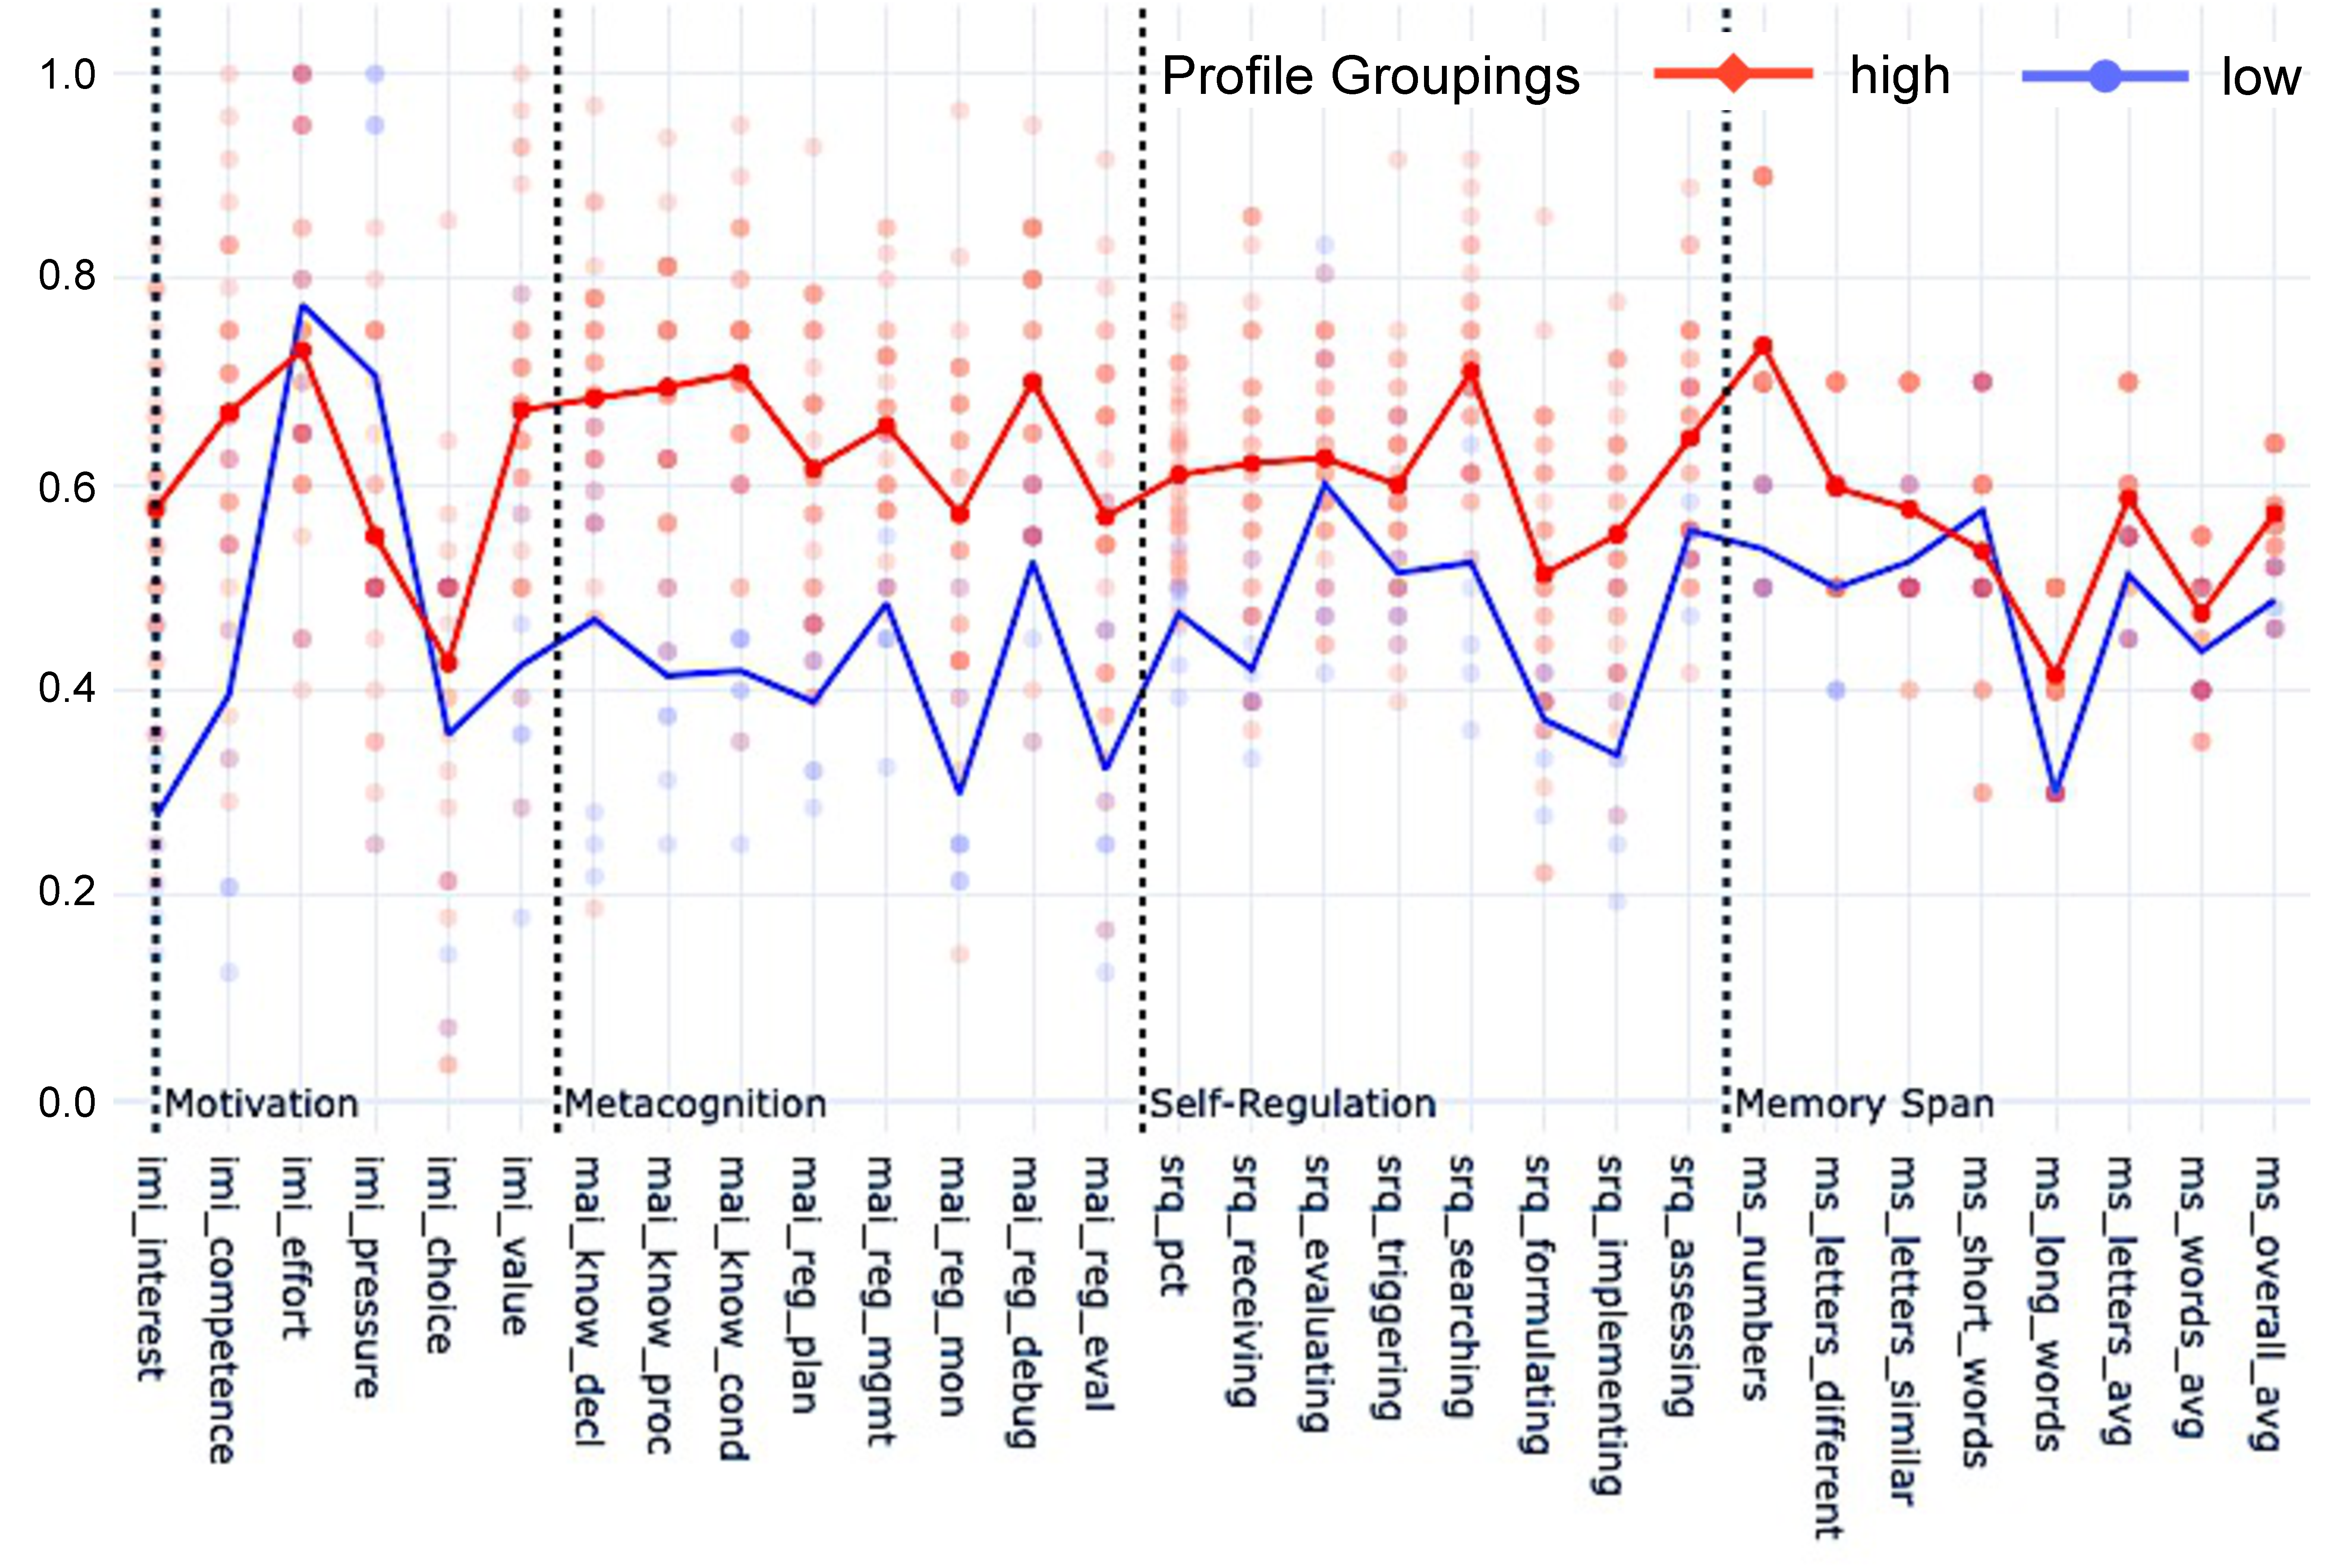
\includegraphics[width=1\linewidth]{figs/lpa-profile-means} 

}

\caption[Groups identified by Latent Profile Analysis.]{Mean Values of Indicator Variables for the two identified groups via Latent Profile Analysis (LPA). The grouping was based on the self-reported values of motivation (IMI), metacognition (MAI), self-regulation (SRQ), and a Memory Span task.}\label{fig:lpa-profile-means}
\end{figure}





According to Ambrose et al. (\protect\hyperlink{ref-ambrose2010howa}{2010}), students' motivation, metacognition, and self-regulation are critical factors that determine, direct, and sustain what they do to learn.
Given our interest in understanding how these traits impact students' searching as learning behaviour, we collected self-perceived reports of all three constructs, via the IMI, MAI, and SRQ questionnaires (Section \ref{sec-method-qsnr1}).
However, it is important to note that these constructs are not single binary variables that can be used to easily group individuals. Rather, they are complex and multidimensional data that serve as observable indicators of a person's underlying latent characteristics.

To cluster participants into meaningful groups based on these multiple constructs, we turned to the educational psychology literature.
\textbf{Latent Profile Analysis (LPA)} is an increasingly popular statistical approach falling under the umbrella of person-centred techniques used in organizational psychology and child development research. It provides a framework for characterizing population heterogeneity in terms of differences across individuals on a set of behaviours or characteristics, as opposed to describing the variability of a single variable. By identifying latent subgroups within a population, LPA enables researchers to gain a more nuanced understanding of the complexity of human behaviour.

The \textbf{person-centred approach} underlying LPA is a departure from traditional variable-centred approaches such as multiple regression analysis. Instead of quantifying the role of particular variables in a study, LPA organizes a population into a finite number of mutually exclusive and exhaustive profiles, each comprising individuals who are similar to one another. In this way, LPA identifies distinct profiles of individuals who exhibit similar patterns of behaviour across multiple variables.

The identification and description of these latent profiles is a crucial step in LPA. Each profile represents a subgroup of individuals who share similar patterns of responses on a set of variables, which can provide insights into the underlying mechanisms driving their behaviour. Furthermore, the identification of the optimal number of profiles to represent a population is a critical issue in LPA. This involves balancing the complexity of the model with its ability to capture meaningful variability in the data, and requires careful consideration of both statistical and substantive criteria.

LPA has several advantages over traditional variable-centred approaches. It allows for a more nuanced understanding of the complexity of human behaviour, particularly in cases where individuals exhibit multiple and diverse patterns of behaviour across different sets of variables.

In the context of information search behaviour, LPA can help to identify distinct groups of individuals who engage in different search strategies or have different search motivations. This can be useful for understanding how people search for information online, what factors influence their search behaviour, and how search behaviour relates to other variables such as task performance, satisfaction, and learning outcomes.

The purpose of this study was to investigate the relationship between individual differences in motivation, metacognition, and self-regulation and search behaviour.
To classify participants into high and low groups based on their scores on these questionnaires, we employed LPA.
LPA is particularly useful when the relationship between variables is not well understood or when it is difficult to determine which variables should be used to classify individuals into groups.
We employed LPA to identify latent profiles of participants based on their scores on the IMI, MAI, and SRQ questionnaires.
LPA is particularly useful when the relationship between variables is not well understood, or when it is difficult to determine which variables should be used to classify individuals into groups.

The results of the LPA showed that there were two distinct groups (latent profiles) of participants based on their scores on the IMI, MAI, SRQ, and MS: a high group and a low group (Figure \ref{fig:lpa-profile-means}). The high group had generally higher average scores on the IMI, MAI, SRQ, and MS compared to the low group, indicating that they were more intrinsically motivated, more aware of their metacognitive processes, and had higher levels of self-regulation.

\begin{figure}

{\centering 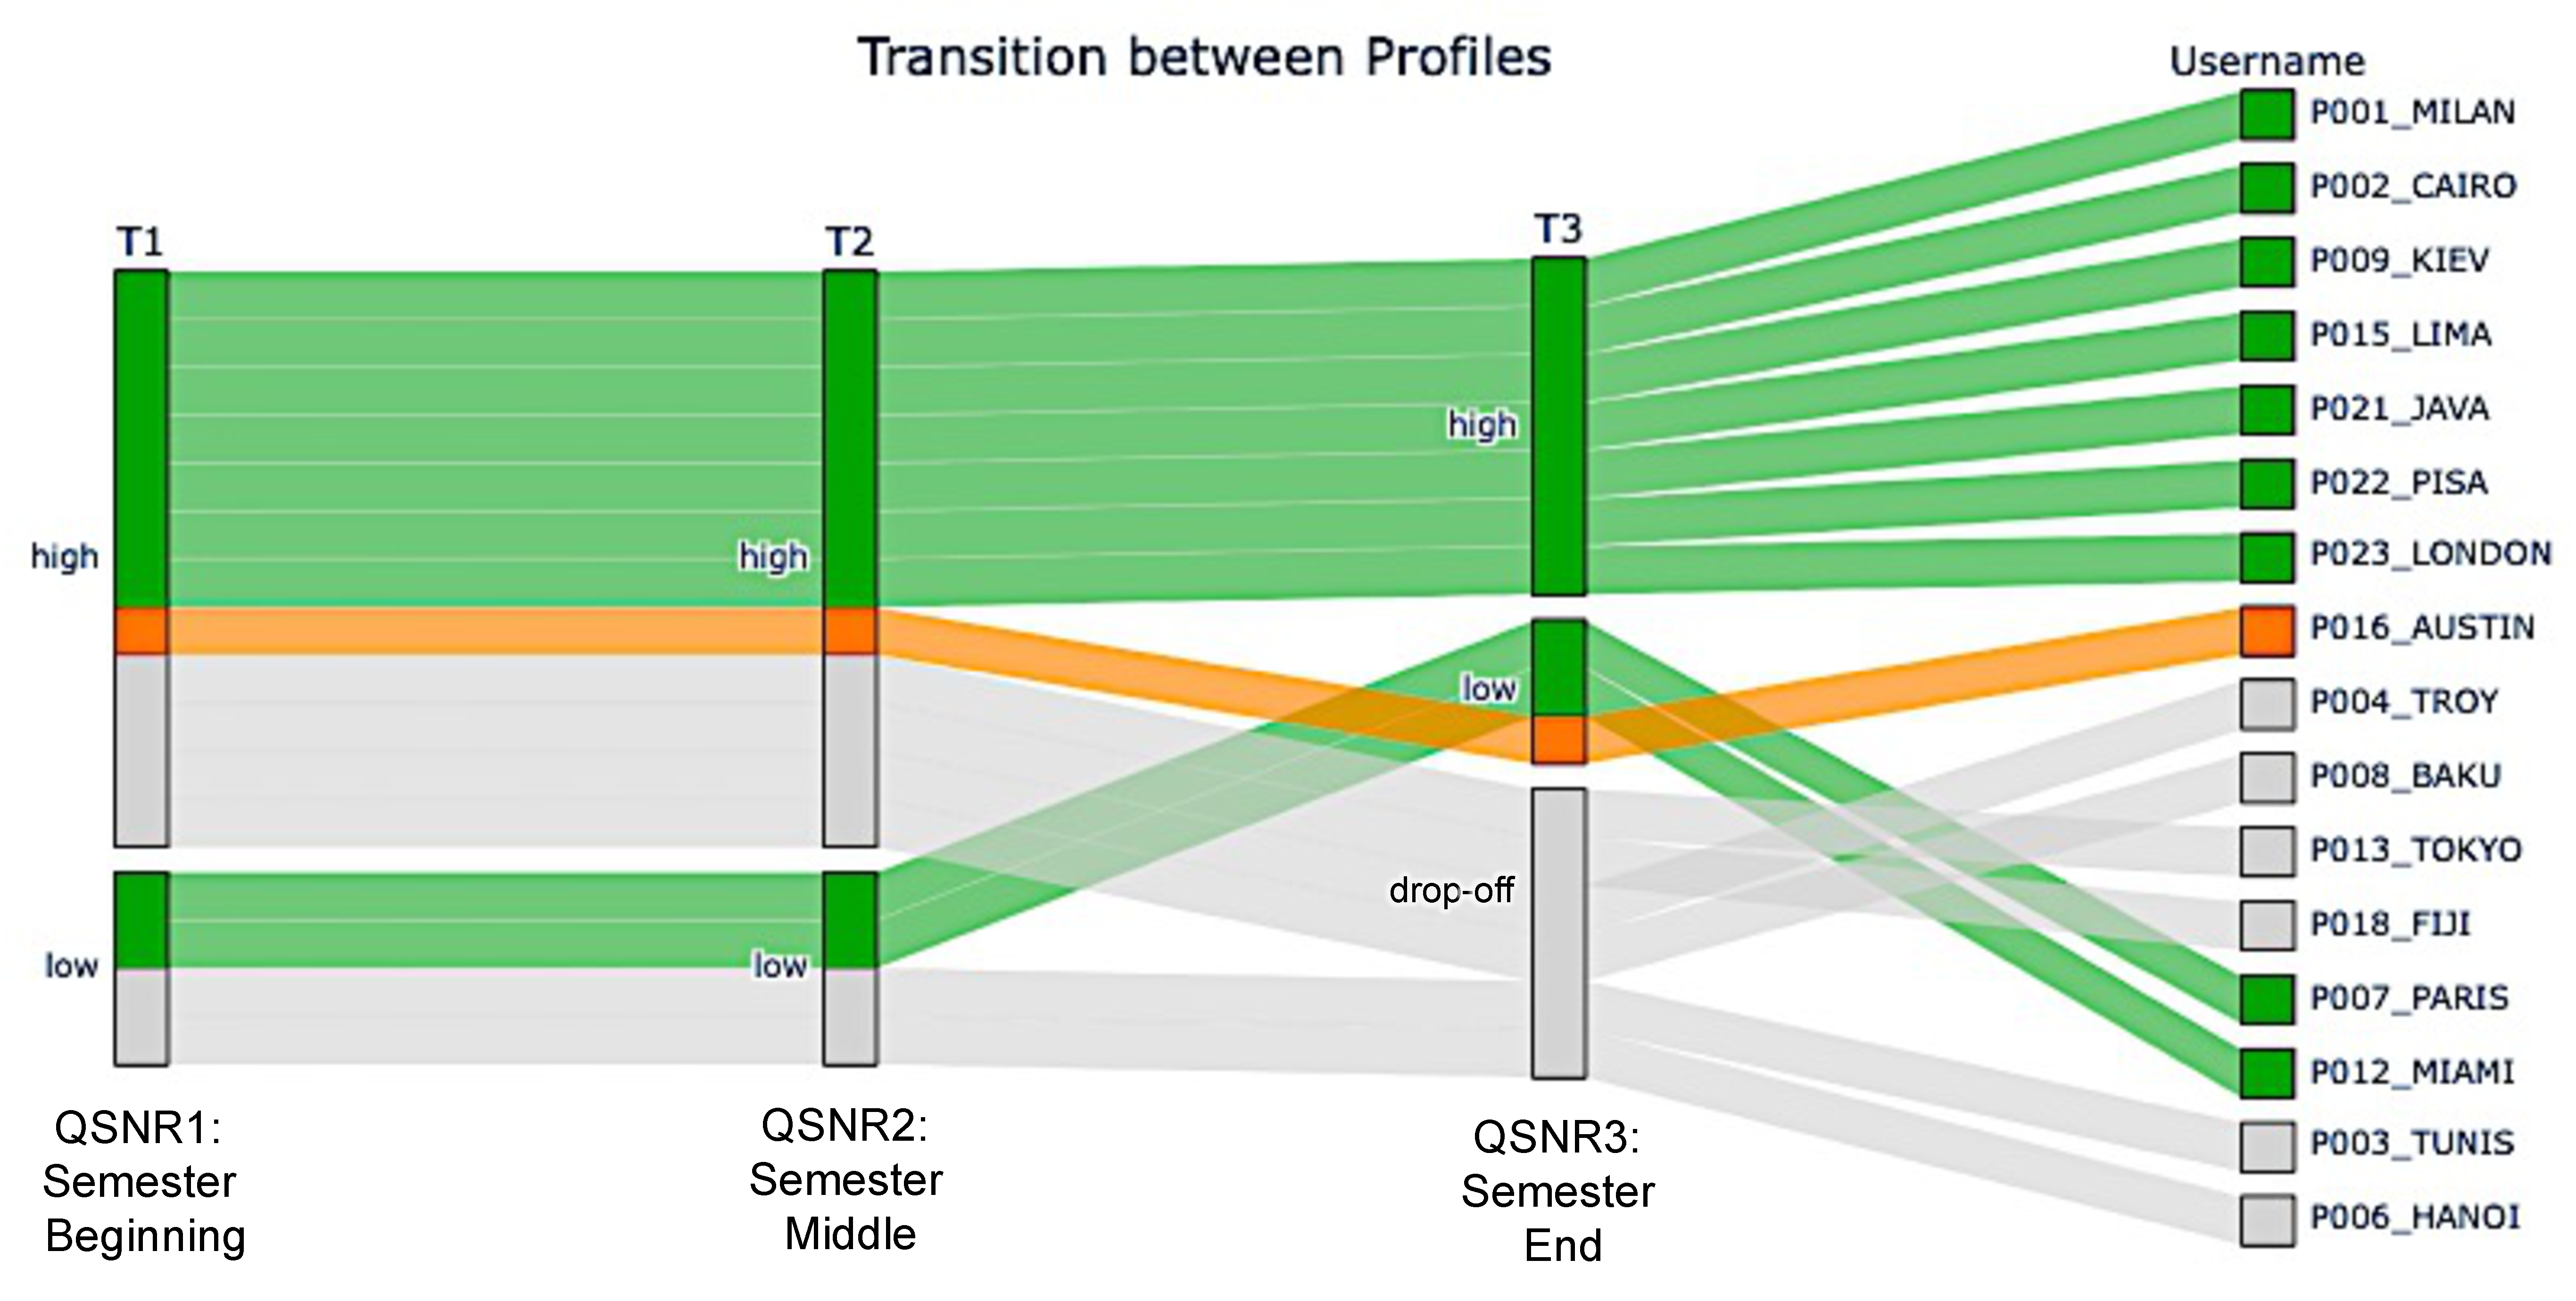
\includegraphics[width=1\linewidth]{figs/lpa-profile-transitions} 

}

\caption[LPA Profile Transitions.]{Diagram illustrating, at different timepoints, how participants stayed within their same high/low LPA profiles (green) or changed profiles (orange). Grey trajectories indicate participants who dropped off and did not complete the study.}\label{fig:lpa-profile-transitions}
\end{figure}





Figure \ref{fig:lpa-profile-transitions} illustrates the memberships in the two groups at different points in time, and how one participant (\texttt{P016\_AUSTIN}) changed group membership at the end of the semester.
12 participants started off the semester (\texttt{QSNR1}) in the high group, while 4 in the low group.
The group membership remained the same in the middle of the semester (\texttt{QSNR2}).
At semester end, 4 participants from the high group and 2 participant from the low group dropped off.
One participant transitioned from high group to low group.
This resulted in 7 participants in the high group and 3 participant in the low group, with no data for 6 participants at the semester end timepoint (\texttt{QSNR3})

In the discussion that follows, all the \textbf{Effect Sizes (ES)} reported as part of Mann Whitney U tests, compare the scores of the low group (first distribution) with those of the high group (second distribution).
In other words, an example effect size \(ES=0.19\) means that there is a 19\% chance that a score from the low group will be greater than the corresponding score from the high group.

\hypertarget{learning-and-search-outcomes}{%
\section{Learning and Search Outcomes}\label{learning-and-search-outcomes}}

\begin{figure}

{\centering 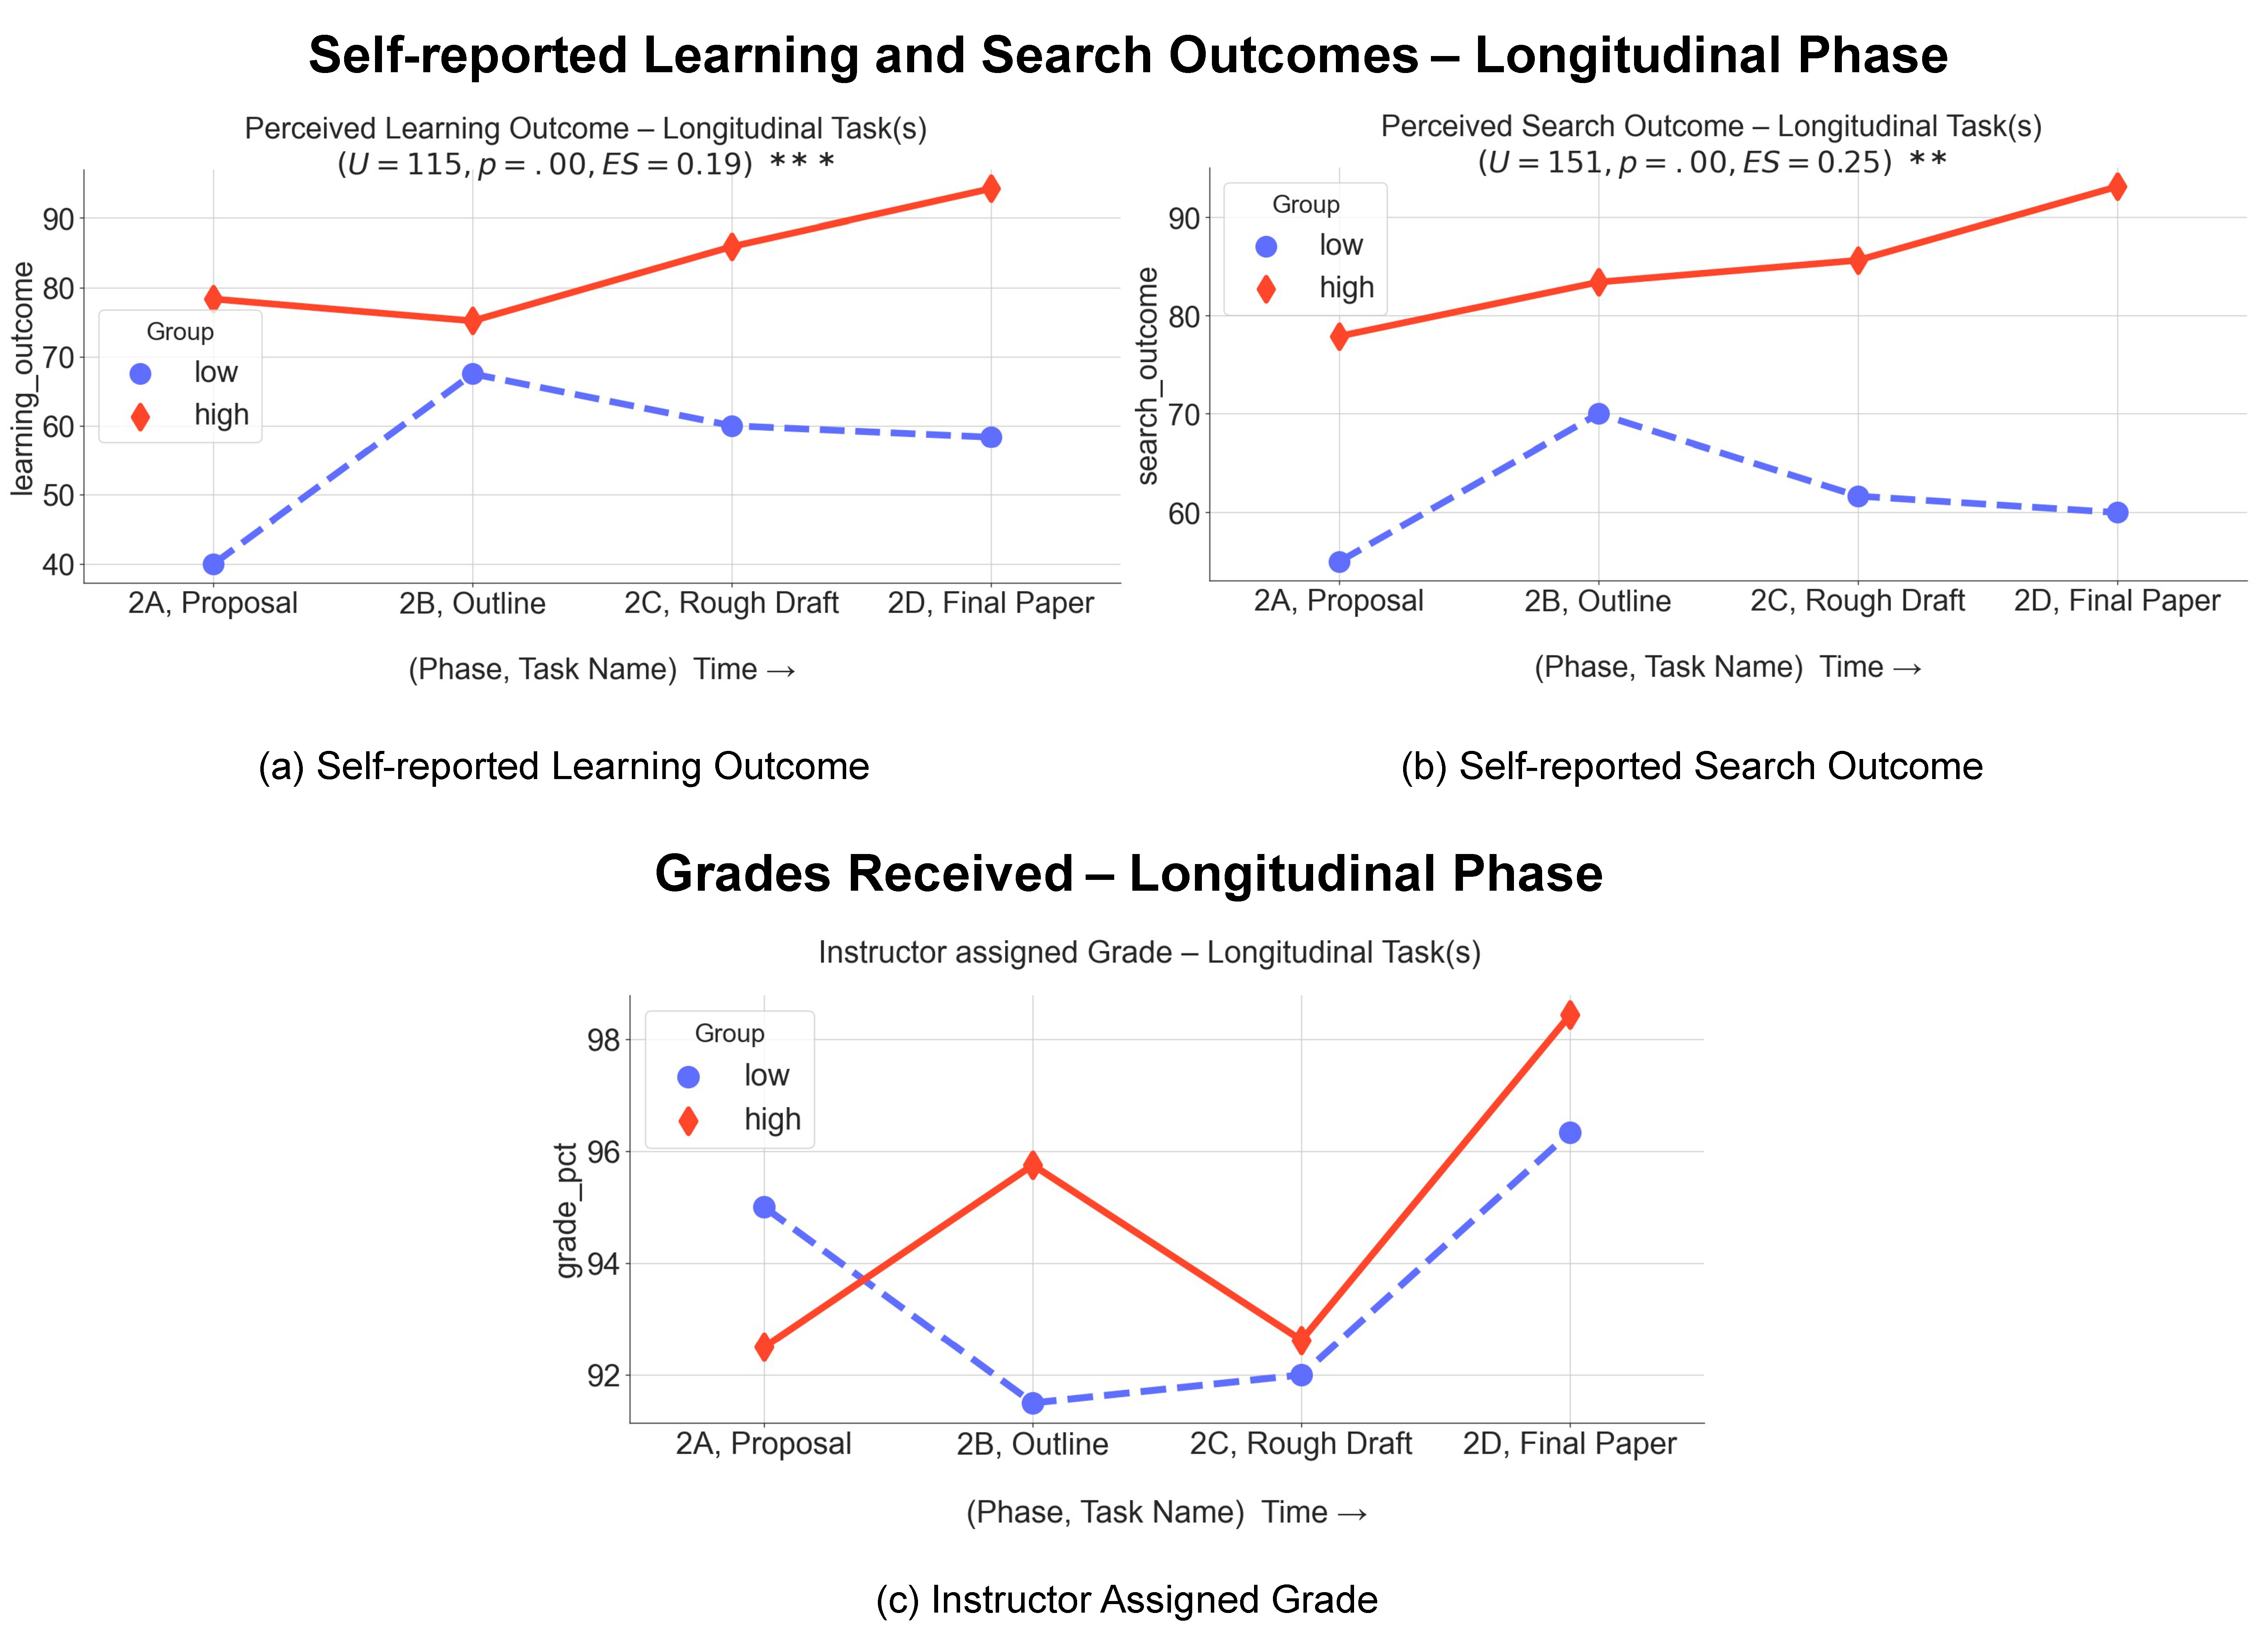
\includegraphics[width=1\linewidth]{figs/rp2-learning-search-outcomes} 

}

\caption[Self-reported learning and search outcomes, and grades received in the longitudinal phase.]{Self-reported learning and search outcomes (a, b), and instructor assigned grades for the high and low groups (c).}\label{fig:rp2-learning-search-outcomes}
\end{figure}





Figure \ref{fig:rp2-learning-search-outcomes} shows the mean values of the self-reported (perceived) learning outcomes (a), self-reported search outcome (b), and instructor assigned grades (c) for the Ethical Dilemma research paper writing task over the semester.
The self-reported learning and search outcomes are inspired from work by Collins-Thompson et al. (\protect\hyperlink{ref-collins2016assessing}{2016}).

We see that the high group had higher levels of perceived learning outcome and perceived search outcome compared to the low group, and these differences were statistically significant: \((U = 115.0, p = .0005, ES = 0.19)\) for the learning outcome, and \((U = 151.0, p = .005, ES = 0.25)\) for the search outcome.
(The effect sizes indicate the probability that a value chosen at random from the low group's scores will be greater than a value chosen at random from the high group's scroes.)

The fact that the high group had statistically significant higher self-reported learning outcomes and self-reported search outcomes suggests that these students had a higher level of motivation, self-regulation, and better time management skills than the low group.
This is because students who are motivated and self-regulated tend to be more efficient and effective in their information searching behaviours, which in turn may lead to better learning outcomes.
Additionally, students in the high group were better at managing their time and resources, allowing them to engage in more thorough and comprehensive information searching activities.
This is corroborated by interview responses as well.
For instance, when asked ``How did you keep track of the sources you found?'\,', a participant in the low group responded:

\begin{quote}
\emph{\ldots in the reference list, I put all the links that I found. I did {[}save the articles{]} at one point. And then before I knew it, \textbf{I had 10 tabs (open)}, and I feel extremely unmotivated. I said, no, I can't do this anymore. \textbf{So I just closed all of them}.}

\emph{And I decided, okay, everything's in the reference list, \textbf{Whatever seems like its relevant. I'll click on it, and I'll see it later}. So I don't have to read 10 different papers. \textbf{I relied too much on the reference list. I throw everything in there}, like okay, I'll deal with you later.}

\hfill --- P007\_PARIS
\end{quote}

In contrast, a participant in the high group responded:

\begin{quote}
\emph{I have a \textbf{separate document} with a table and \textbf{three columns}, one for the \textbf{in-line citation}, so I could just easily copy and paste it. And then the middle was \textbf{direct quotes}. And then the (last column) was \textbf{notes} that are like sentences, what I wanted to say. And so that's how I organize my (sources).}

\hfill --- P021\_JAVA
\end{quote}

The instructor assigned grades for the high group also generally stayed higher than the low group (except for the Proposal stage). However, the differences were small.
This may indicate that the instructors' grading criteria may not have fully captured the impact of information searching behaviours on learning outcomes.
This is because the instructor's grading criteria may have been focused more on the content of the research paper, rather than the process of information searching. As a result, students who were more effective in their information searching behaviours may not have received a higher grade, even if their research paper was of higher quality.
Another possibility is that the grading process may have been liberal towards the students.

Collins-Thompson et al. (\protect\hyperlink{ref-collins2016assessing}{2016}) reported that ``searchers' perceived learning outcomes closely matched their actual learning outcomes'' and this was also indirectly correlated with their information search behaviours in terms of dwell time on documents.
Let us examine in the following sections how the findings from the LongSAL study compare and contrast with those reported by Collins-Thompson et al. (\protect\hyperlink{ref-collins2016assessing}{2016}) and others.

\hypertarget{q-query-formulations}{%
\section{Q: Query Formulations}\label{q-query-formulations}}

\hypertarget{length-and-count-of-queries-per-search-task}{%
\subsection{Length and Count of Queries per Search Task}\label{length-and-count-of-queries-per-search-task}}

\begin{figure}

{\centering 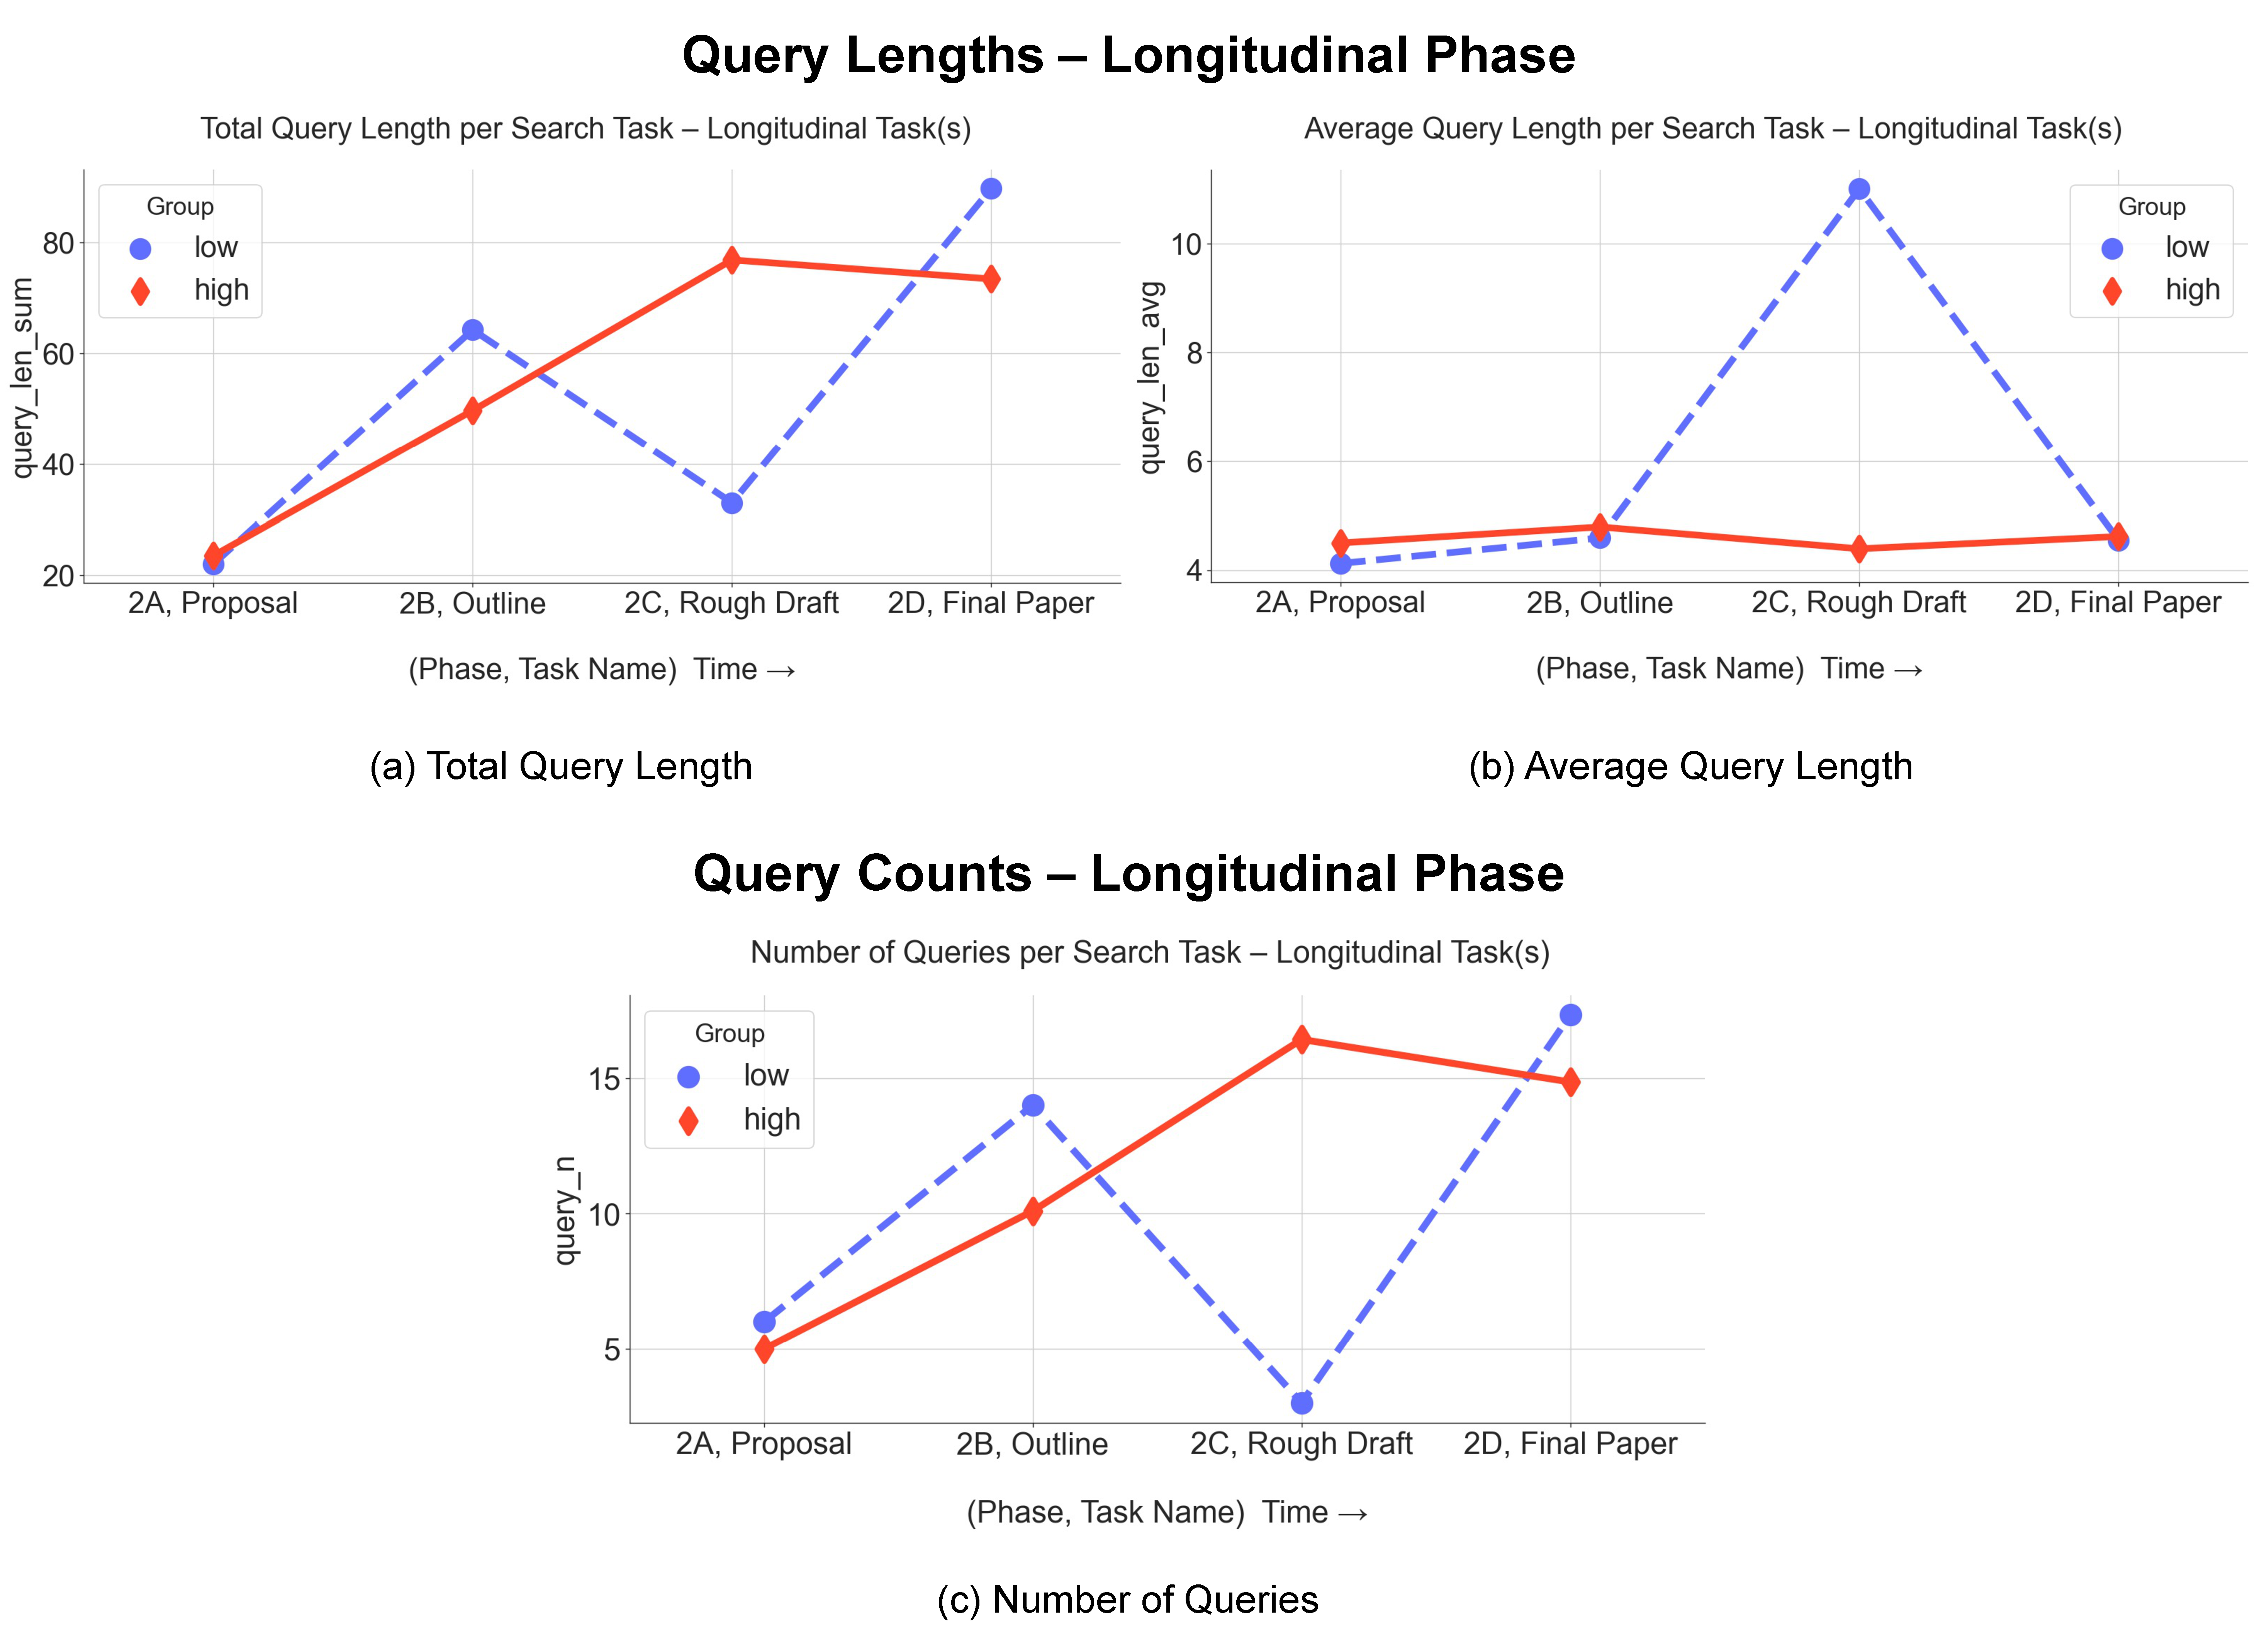
\includegraphics[width=1\linewidth]{figs/rp2-query-length-count} 

}

\caption[Query length and counts -- longitudinal phase.]{Lengths and count of queries for each search task in the Longitudinal Phase.}\label{fig:rp2-query-length-count}
\end{figure}





\textbf{Query length} was operationalized as the number of terms (words separated by spaces) in the search query that participants submitted to the search engines or other information retrieval sites.
Query length can vary from a single word to several phrases or a complete sentence.
Longer search queries may indicate a more specific or complex information need, while shorter search queries may be more general or broad in scope.
\textbf{Queries count} per search task refers to the number of separate queries or search attempts that a participant issued in order to complete a task.
This measure may vary depending on the complexity of the information need, the user's level of expertise with the search system, and other factors.

Figure \ref{fig:rp2-query-length-count} (a) and (b) shows the differences in total and average query length of the high and low groups, while Figure \ref{fig:rp2-query-length-count} (c) illustrates the number of queries issued, at different stages of writing the research paper. The low group demonstrated a zig-zag pattern in their \textbf{total query length} and query count over the semester, with a low start at proposal, followed by a peak at outline, a dip at rough draft, and a peak at Final Paper.
The high group had a steady increase in total query length and query count, from proposal to outline to rough draft, and took a very gentle dip (or remained steady) at final paper stage.
Comparing the total query length and query count to the \textbf{average query length} (Figure \ref{fig:rp2-query-length-count} (b)), we see that the high group maintained a steady 4-5 terms per query throughout the semester, whereas the low group had a jump to more than 10 terms per query in the rough draft stage.

The low group issued few short queries during the proposal, many short queries during the outline, very few long queries during the rough draft, and again many short queries during the final paper phase.
On the other hand, the high group kept issuing a steadily increasing count of similar-length (short) queries throughout the semester.

Combining these results we can posit that the low group demonstrated signs of struggling throughout the semester (\protect\hyperlink{ref-hassan2014struggling}{Hassan et al., 2014}).
These students may have struggled to effectively search for information at the beginning of the semester, but then increased their search efforts as the deadlines approached. The fact that they issued few long queries during the rough draft phase may indicate that they were not able to effectively refine their search strategies to find more relevant and valuable information.
In contrast, the high group's pattern of issuing a steadily increasing count of similar-length (short) queries throughout the semester suggests that these students may have had a more consistent and effective search strategy. They may have been better able to refine their search strategies over time, which allowed them to find more relevant and useful information throughout the different stages of the research paper writing process.

\hypertarget{query-reformulation-types-qrts}{%
\subsection{Query Reformulation Types (QRTs)}\label{query-reformulation-types-qrts}}

\begin{figure}

{\centering 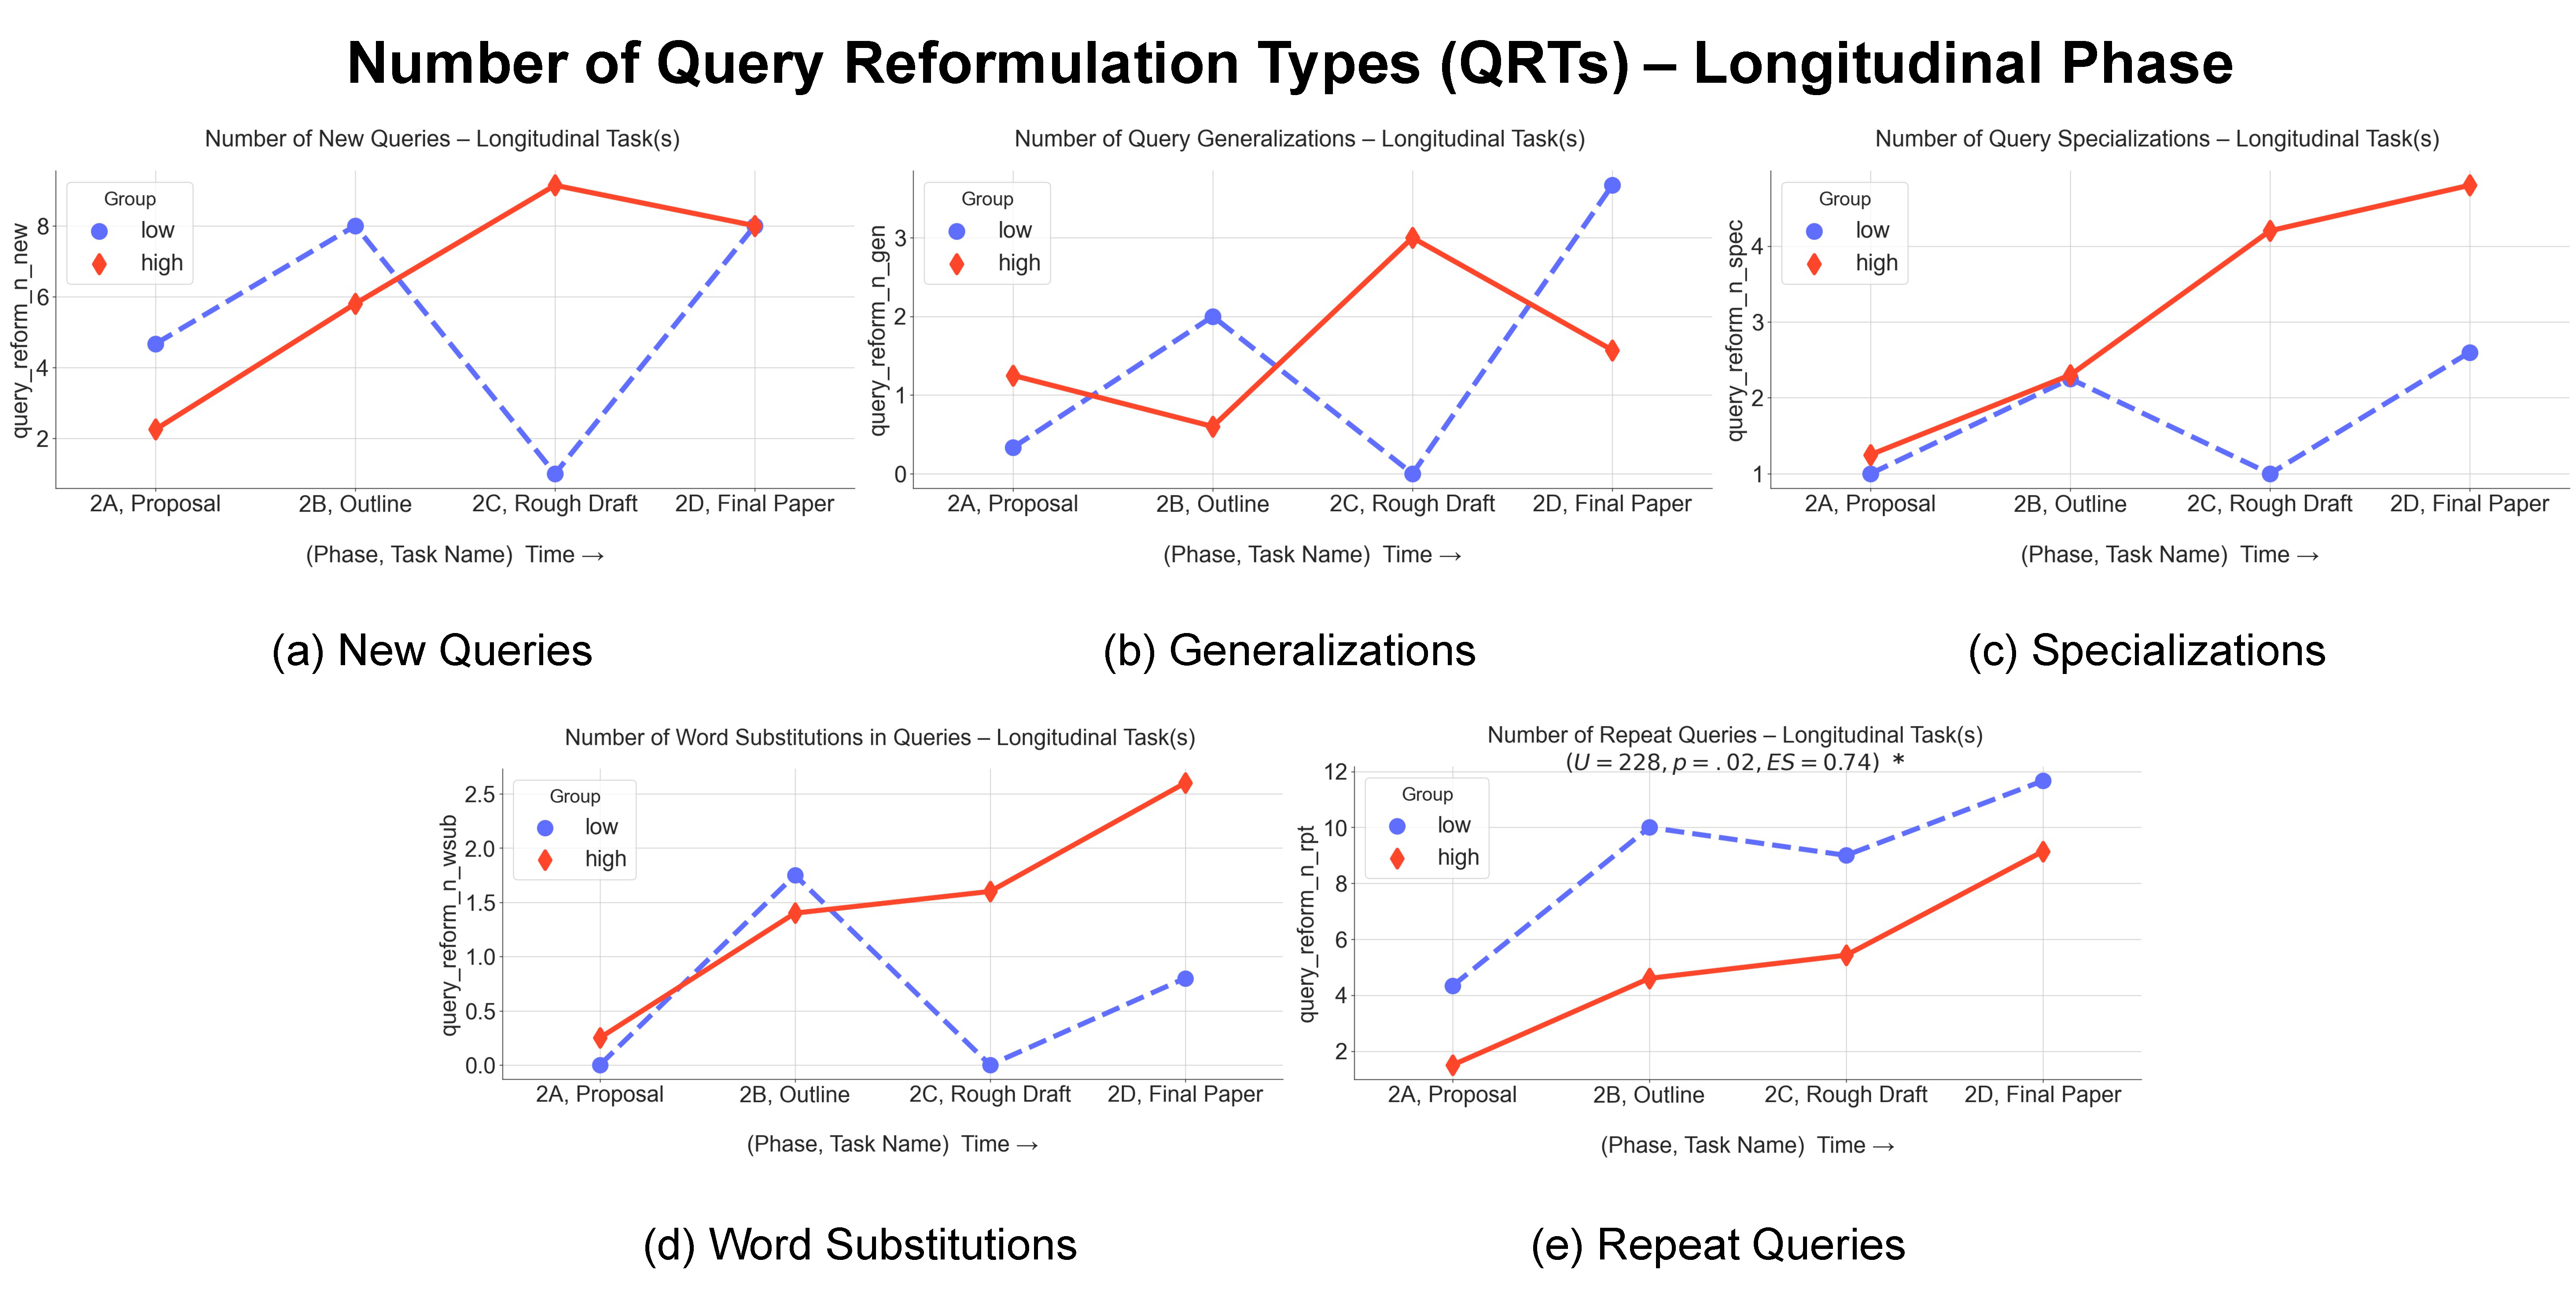
\includegraphics[width=1\linewidth]{figs/rp2-qrt} 

}

\caption[Query reformulation counts for longitudinal phase.]{Number of different query reformulation types (QRTs) as per taxonomy proposed by C. Liu et al. (\protect\hyperlink{ref-liu2010analysis}{2010}).}\label{fig:rp2-qrt}
\end{figure}





Query reformulation refers to the process of modifying or refining a search query in order to improve the relevance of search results and better match the user's information needs (Section \ref{sec-bg-search-query}).
Query reformulation typically occurs due to a searcher's improved understanding of how to better translate their information need into a search query.
Using the taxonomy proposed by C. Liu et al. (\protect\hyperlink{ref-liu2010analysis}{2010}) (Figure \ref{fig:res-Q-QRT-txnmy}), we classified each previous-next query pair issued by participants into one of the five query reformulation types (QRTs):
New,
Generalization,
Specialization,
Word Substitution,
and
Repeat.

We faced a challenge in disentangling \textbf{Repeat} queries from ``hub-and-spoke'' behaviour, where the user goes back and forth between a SERP and different content page by using the browser's forward and back buttons \footnote{The SERP is the hub, which represents the initial point of inquiry, while the spokes represent the subsequent branches of exploration along different content pages. This search behaviour is often used when users have a general idea of the topic they are interested in, but need to explore different facets of the topic to narrow down their search and find relevant information.}.
Each back button press on the browser (to go back to the SERP from a content page) meant a fresh HTTP GET request was sent to the search engine.
This resulted in YASBIL logging the move as a resubmission of the query.
So for the discussions that follows, \textbf{``Repeat'' refers to repeat queries combined with hub-and-spoke behaviour.}.

The counts of the five QRTs are presented in Figures \ref{fig:rp2-qrt} (a) through (e).
For the low group, the trend of counts followed similarly from their trends of query counts and total query lengths (Figures \ref{fig:rp2-query-length-count} (a) and (c)), with varying intensities: alternating between high and low values at successive points in the semester.
For the high group, except Query Generalizations -- which followed a zig-zag pattern -- all the other QRTs showed an overall increase in count throughout the semester.

The high group issued the most new queries and generalized queries while writing the rough draft. In contrast they had the highest counts of specializations and word substitutions while writing the final paper.
The low group, on the other hand, had their lowest counts of all QRTs, except repeat, while writing the rough draft.
The most interesting tresnd is that of Query Generalizations (Figure \ref{fig:rp2-qrt}(b)), where the high group and low group demonstrated diametrically opposite behaviour: maxima at outline and final paper for the low group, whereas minima at those stages for the high group.
The high group also issued significantly fewer repeat queries (aka hub and spoke behaviour) throughout the semester, compared to the low group \((U = 228.0, p = .02, ES = 0.74)\).

The low group's fewer counts of all QRTs while writing the rough draft suggests that they may have struggled to effectively reformulate their queries throughout the different stages of the research paper writing process, perhaps due to the complexity and depth of the research required for the tasks.
The low group may have had more difficulty refining and targeting their search queries, resulting in more new and repeated queries at the final stage of the paper writing process.
They may also have had more difficulty with the conceptualization of their research question or topic, leading to more generalizations and fewer specializations in their queries.
Additionally, their higher use of repeat queries (or hub and spoke behaviour) may indicate that they were relying on a limited set of sources or search terms, which may have limited their ability to find new and relevant information.

The high group, however, had a different pattern of query reformulation compared to the low group.
They had their highest counts of new queries and query generalizations in the Rough Draft Phase, and most specialization, word substitutions, and repeat queries while writing the Final Paper.
This indicates that their queries were more exploratory in the early part of the semester, and became more precise and refined in the later parts of the semester.
They may have been more proactive in identifying new avenues for research earlier in the semester.
The highest count of query generalizations during the writing of the rough draft may suggest that they were better able to synthesize and generalize information from their sources at an earlier stage in the writing process.
The high group may also have been better able to refine their search queries through word substitutions, which peaked while writing the final paper, indicating a greater level of precision and focus in their information seeking behaviour.
In contrast, the low group had their highest count of repeat queries during the outline and final paper, indicating that they may have had more difficulty finding and retaining relevant information throughout the research process.

Interview responses from the participants also support these quantitative.
When asked which stage of the project needed the most amount of searching -- proposal, outline, rough draft, or final paper -- a participant in the low group responded:

\begin{quote}
\emph{Definitely the \textbf{final one}. Not only do I have to find the extra 10 source material, because in the rough draft, I only need 10. So not only do \textbf{I have to find 10 new ones}, I need to go back to look at the old 10 sources that I had before because \textbf{I don't remember what they're about anymore}.}

\hfill --- P007\_PARIS
\end{quote}

On the other hand, a participant in the high group responded:

\begin{quote}
\emph{searching, probably in the \textbf{outline} stage, but the most \textbf{analyzation} of those sources came in the \textbf{rough draft} stage, and then the \textbf{final is just expanding} upon that.}

\hfill --- P021\_JAVA
\end{quote}

From the above observations, we posit that the high group were more effective in their query reformulation strategies.
Specifically, the high group were better able to identify new information needs as they worked on the rough draft, and then refine and specialise their queries as they worked on the final paper.
This ability to adapt and refine their queries may have allowed them to find more relevant and useful information, which in turn may have contributed to their higher self-perceived learning and search outcomes.

\hypertarget{sec-res-phase2-query-H}{%
\subsection{Entropy of Query Reformulation Types}\label{sec-res-phase2-query-H}}

\begin{figure}

{\centering 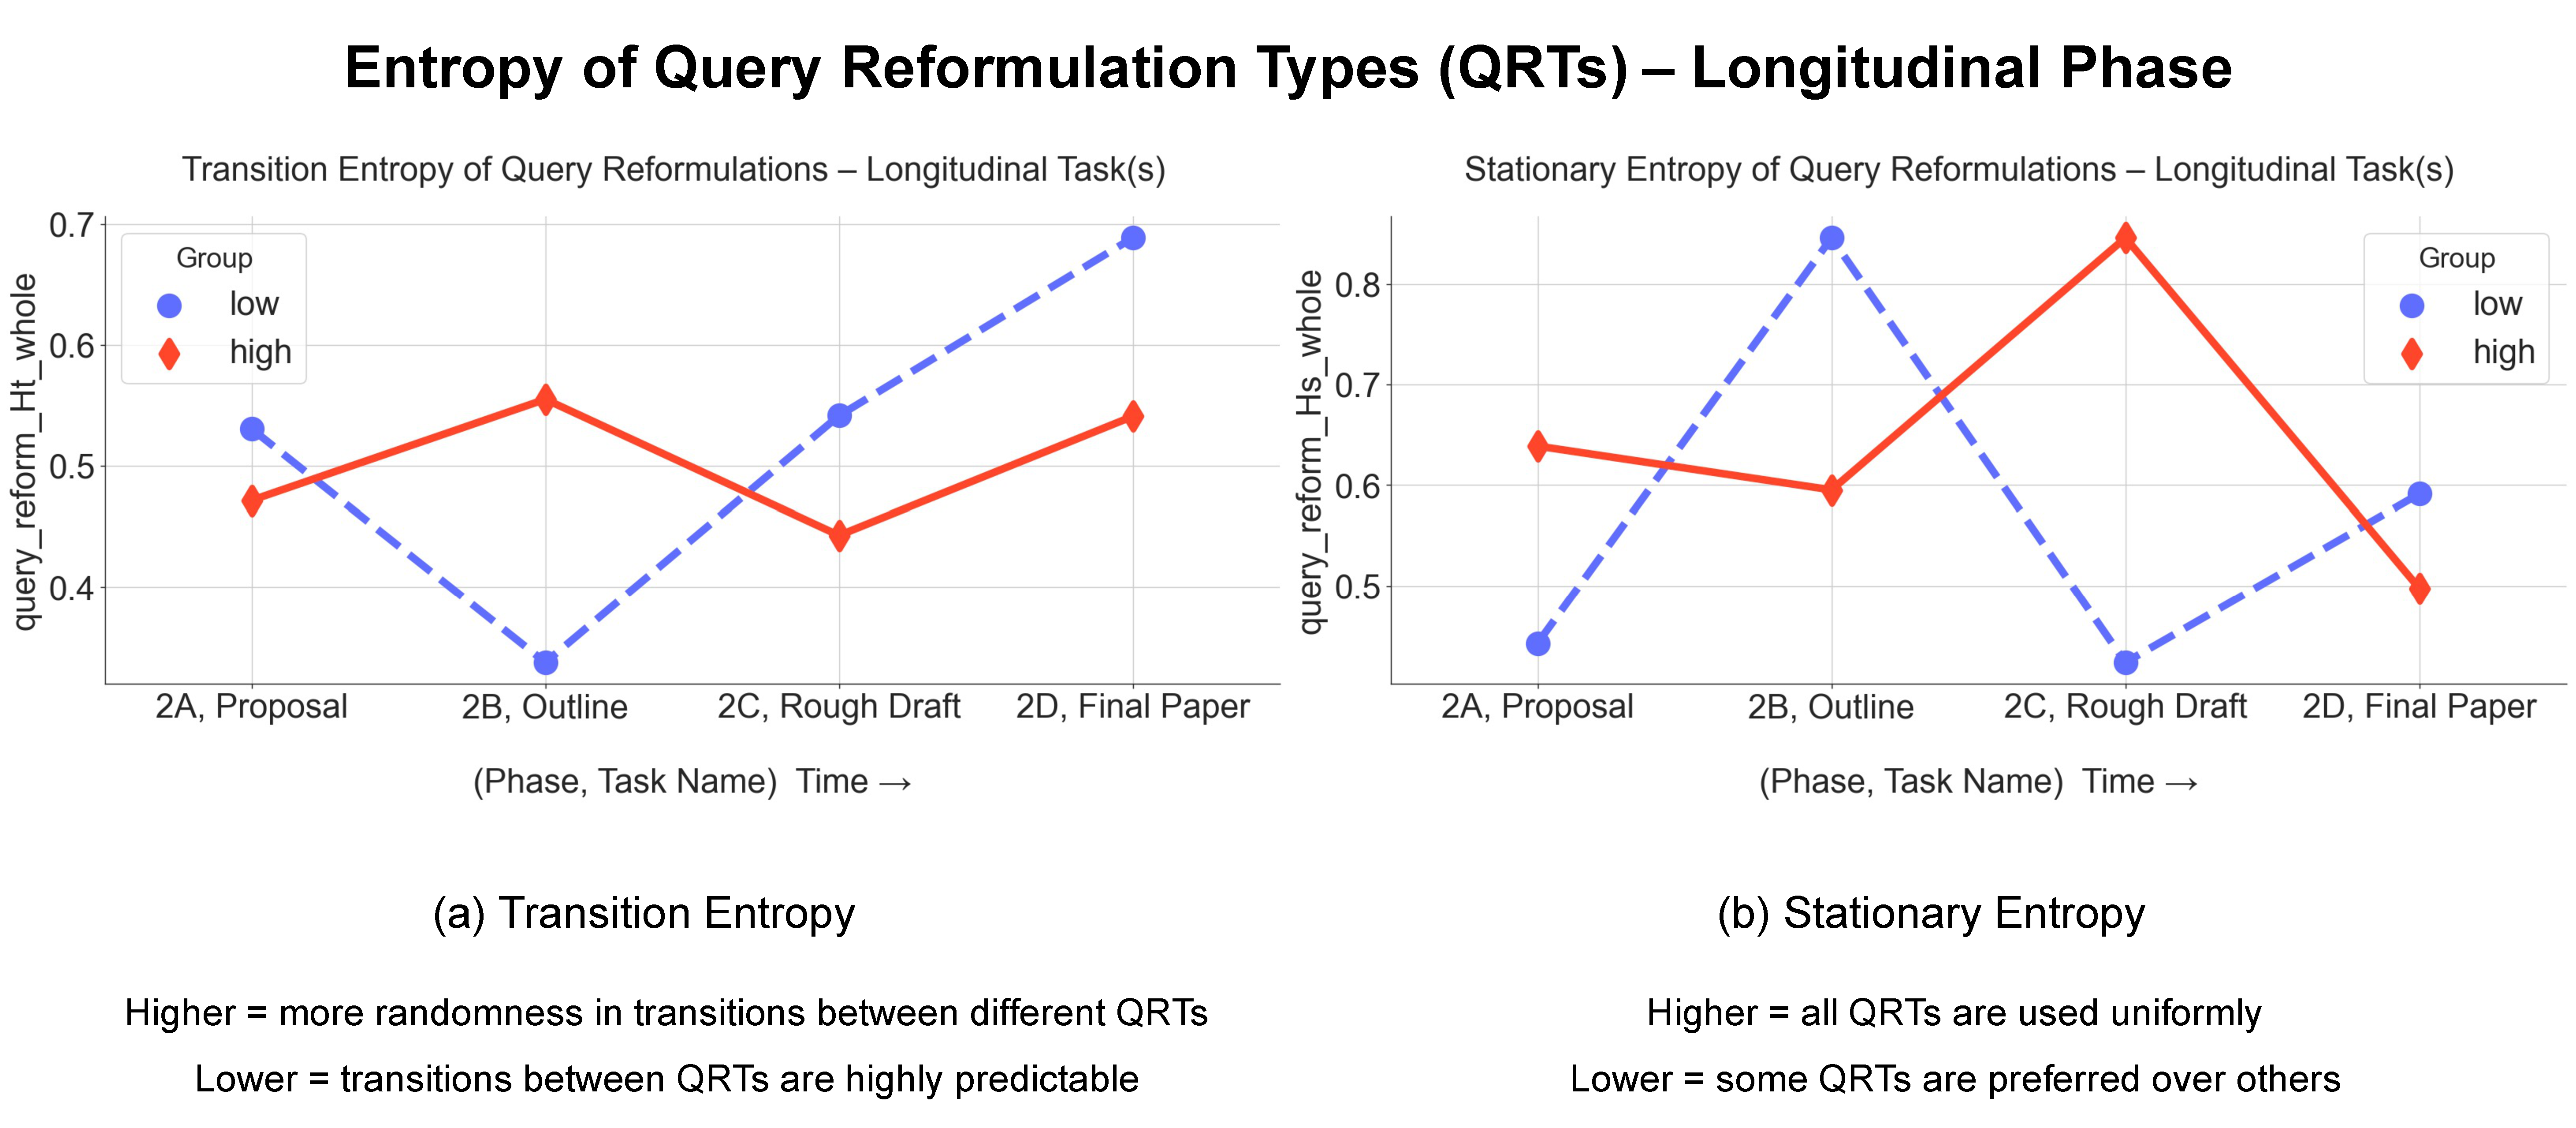
\includegraphics[width=1\linewidth]{figs/rp2-qrt-entropy} 

}

\caption[Entropy of Query Reformulation Types for the Longitudinal Phase.]{Stationary and transition entropies of query reformulation type (QRT) sequences.}\label{fig:rp2-qrt-entropy}
\end{figure}





Entropy is a measure of the diversity or unpredictability of a sequence of events. In the context of search queries, entropy can be used to quantify the variability or randomness of the query reformulations issued by participants.
Transition analysis and entropy helps to cover differences in disparate tasks and activities.
Inspired by previous works in analysing eye-movement sequences (\protect\hyperlink{ref-krejtz2014entropy}{Krejtz et al., 2014}, \protect\hyperlink{ref-krejtz2015gaze}{2015}) and search tactics sequences (\protect\hyperlink{ref-he2016beyond}{He et al., 2016}), we employed a similar entropy analysis of query reformulation sequences, and search tactic patterns of the participants.

For query reformulations, the possible set of states were the five query reformulation types:
Generalization, Specialization, Word Substitution, Repeat, and New.
If we consider a sequence of query reformulations issued by a participant
(e.g., \emph{New -\textgreater{} New -\textgreater{} Specialization -\textgreater{} Specialization -\textgreater{} Word Substitution -\textgreater{} Generalization})
then this sequence can be considered as a first order Markov chain, wherein, the next step in the chain depends only on the current state.
Entropy analysis on these Markov chains quantifies how predictable the states are, and yields two categories of uncertainty measures: transition entropy, \(H_t\), and stationary entropy \(H_s\).
Similar stationary and transition entropy measures can be obtained for sequences of search tactics.

Guided by the above, we carried out entropy analysis of query reformulation sequences produced by the participants.
In the context of query reformulations, the maximum \textbf{transition entropy}, \(s \log s\), can be reached when there is an equal probability of switching between each of the \(s = 5\) states, or QRTs (query reformulation types).
The minimum transition entropy (0) is achieved in a fully deterministic Markov chain, where all transition probabilities are either 1 or 0.
This means that with a higher transition entropy there is more randomness in the participant's transitions between different QRTs.
This randomness is an indication that the participants do not have a clear progression from one QRT to another.
On the other hand, a lower transition entropy indicates that the participant's transition between QRTs are highly predictable.
\textbf{Stationary entropy} is calculated from the distribution of QRTs.
A higher stationary entropy value indicates that the QRTs were used uniformly, while a lower stationary entropy indicates that some QRTs are preferred over others.
Values of stationary entropy vary between 0 and \(\log s\), where \(s\) is the number of possible states (QRTs)\footnote{This explanation is adapted from He et al. (\protect\hyperlink{ref-he2016beyond}{2016})}.
All the entropy values presented in this chapter were normalized by their theoretical maximums, for equivalent comparison across different tasks.

The transition entropy of query reformulations followed interesting patterns for the low and high groups (Figure \ref{fig:rp2-qrt-entropy}(a)).
The low group had a V-shaped pattern showing a decrease in transition entropy from proposal to outline, then an increase from outline to rough draft to final paper.
On the other hand, the high group had a zig-zag pattern, with low transition entropy during the proposal, an increase during the outline, a decrease during the rough draft, and then another increase during the final paper.
This indicates that the low group had the least randomness in query reformulation strategies during the outline, while the high group had the most randomness at this stage.
Subsequently, the randomness in the high group decreased, whereas that in low group increased.
This suggests that during the outline stage, the low group had a more structured approach to query reformulations, compared to the high group.
However, as the semester progressed, the low group's approach became more random, while the high group's approach became structured.
These pattern suggests that the low group may have struggled to adapt their query reformulation strategies as they moved through the different stages of writing the paper, while the high group was more able to adjust their strategies and maintain a predictable structure in their approach.

The stationary entropy of query reformulations of the low and high groups varied over the different phases of the research paper writing process as well (Figure \ref{fig:rp2-qrt-entropy}(b)).
The low group's stationary entropy reached its maximum value at the outline phase, whereas that for the high group became maximum at the rough draft phase.
This indicates that these two groups had distinct information searching behaviours throughout the writing process.
The low group tried out all possible types of query reformulations during the outline (as we saw from the query reformulation counts), and then settled on using repeat queries (or hub and spoke behaviour) more, during the rough draft phase.
This lowered their stationary entropy at the rough draft phase, and may have limited their ability to find new and relevant information during the later stages of the writing process.

In contrast, the high group employed all the types query reformulations with equal probability during rough draft phase (Figure \ref{fig:rp2-qrt}), resulting in a higher stationary entropy value.
The increase in the high group's stationary entropy from outline to rough suggests that they were exploring a broader range of topics and concepts at this stage of the writing process, which may have allowed them to identify more relevant and useful information.
The subsequent decrease in stationary entropy from rough draft to final paper suggests that they were able to narrow down their focus and consolidate their understanding of the subject-matter as they progressed, which may have contributed to their higher self-perceived learning and search outcomes.

\hypertarget{sec-res-url-categorization}{%
\section{URL Categorization for Analysing Interactions}\label{sec-res-url-categorization}}

In order to understand the relationship between users' information search behavior and the type of webpages they visit, we needed to categorize webpages into different types. To accomplish this, we developed a classification system based on URL patterns.

URL patterns were first extracted from the web browsing data collected in our study. These URL patterns contain information about the structure and content of each webpage visited by the users. Based on this information, we were able to classify each URL present in the log data into the following hierarchical taxonomy:

\begin{itemize}
\tightlist
\item
  \textbf{\texttt{L}}: Search Result Pages, i.e., a \textbf{L}ist of Information Objects

  \begin{itemize}
  \tightlist
  \item
    \textbf{\texttt{L.PUB}}: Publication Search Results, e.g., on university library websites, digital libraries, Google Scholar, etc.
  \item
    \textbf{\texttt{L.WEB}}: Web Search Engine Result Pages (SERPs)
  \end{itemize}
\item
  \textbf{\texttt{I}}: Content pages, i.e., Individual \textbf{I}nformation Objects

  \begin{itemize}
  \tightlist
  \item
    \textbf{\texttt{I.PUB}}: Academic Publications
  \item
    \textbf{\texttt{I.WEB}}: Webpages that have the potential to provide relevant (academic) information for the search task, but are not publication. E.g., Wikipedia articles, relevant blog posts, government and non-profit websites, etc. Some of them were classified automatically (e.g., Wikipedia), while others were classified after manual inspection.
  \end{itemize}
\item
  \textbf{\texttt{MISC}}: URLs for webpages that did not fit in any of the above category
\end{itemize}

To identify search engine result pages, we looked for URLs that contained URL query parameters such as \texttt{q} (Google, Bing), \texttt{search}, \texttt{query}, or \texttt{k} (Yahoo) along with specific strings associated with popular search engines such as Google or Bing.
We also identified content pages by looking for URLs that contained strings such as ``\texttt{article}'', ``\texttt{blog}'', or ``\texttt{news}''.
Scientific peer-reviewed publications were identified based on URLs that contained specific strings associated with academic publishers or databases (ACM DL, Elsevier, Scopus, Springer etc.), while Wikipedia articles were identified by their URLs containing the string ``\texttt{wikipedia}'' in the hostname.
Library websites were identified by URLs that contained terms such as ``library'', ``catalogue'', or ``database'' as well as specific strings associated with major library systems (e.g., UT Austin uses Primo VE system from Ex Libris). Finally, we used the catch-all category \texttt{MISC} to identify other types of webpages that did not fit into any of the other categories.

The URL-based classification system provided a useful way to categorize webpages based on their type, allowing us to gain insights into how users' search behaviour varies across different types of webpages. By analysing the patterns of webpage types visited by users during their information search process, we were able to identify which types of webpages were most commonly visited and how they related to users' search behaviour.

\hypertarget{l-interaction-with-lists-search-results-source-selection}{%
\section{L: Interaction with Lists / Search Results -- Source Selection}\label{l-interaction-with-lists-search-results-source-selection}}

\hypertarget{number-of-clicks-per-query}{%
\subsection{Number of Clicks per Query}\label{number-of-clicks-per-query}}

\begin{figure}

{\centering 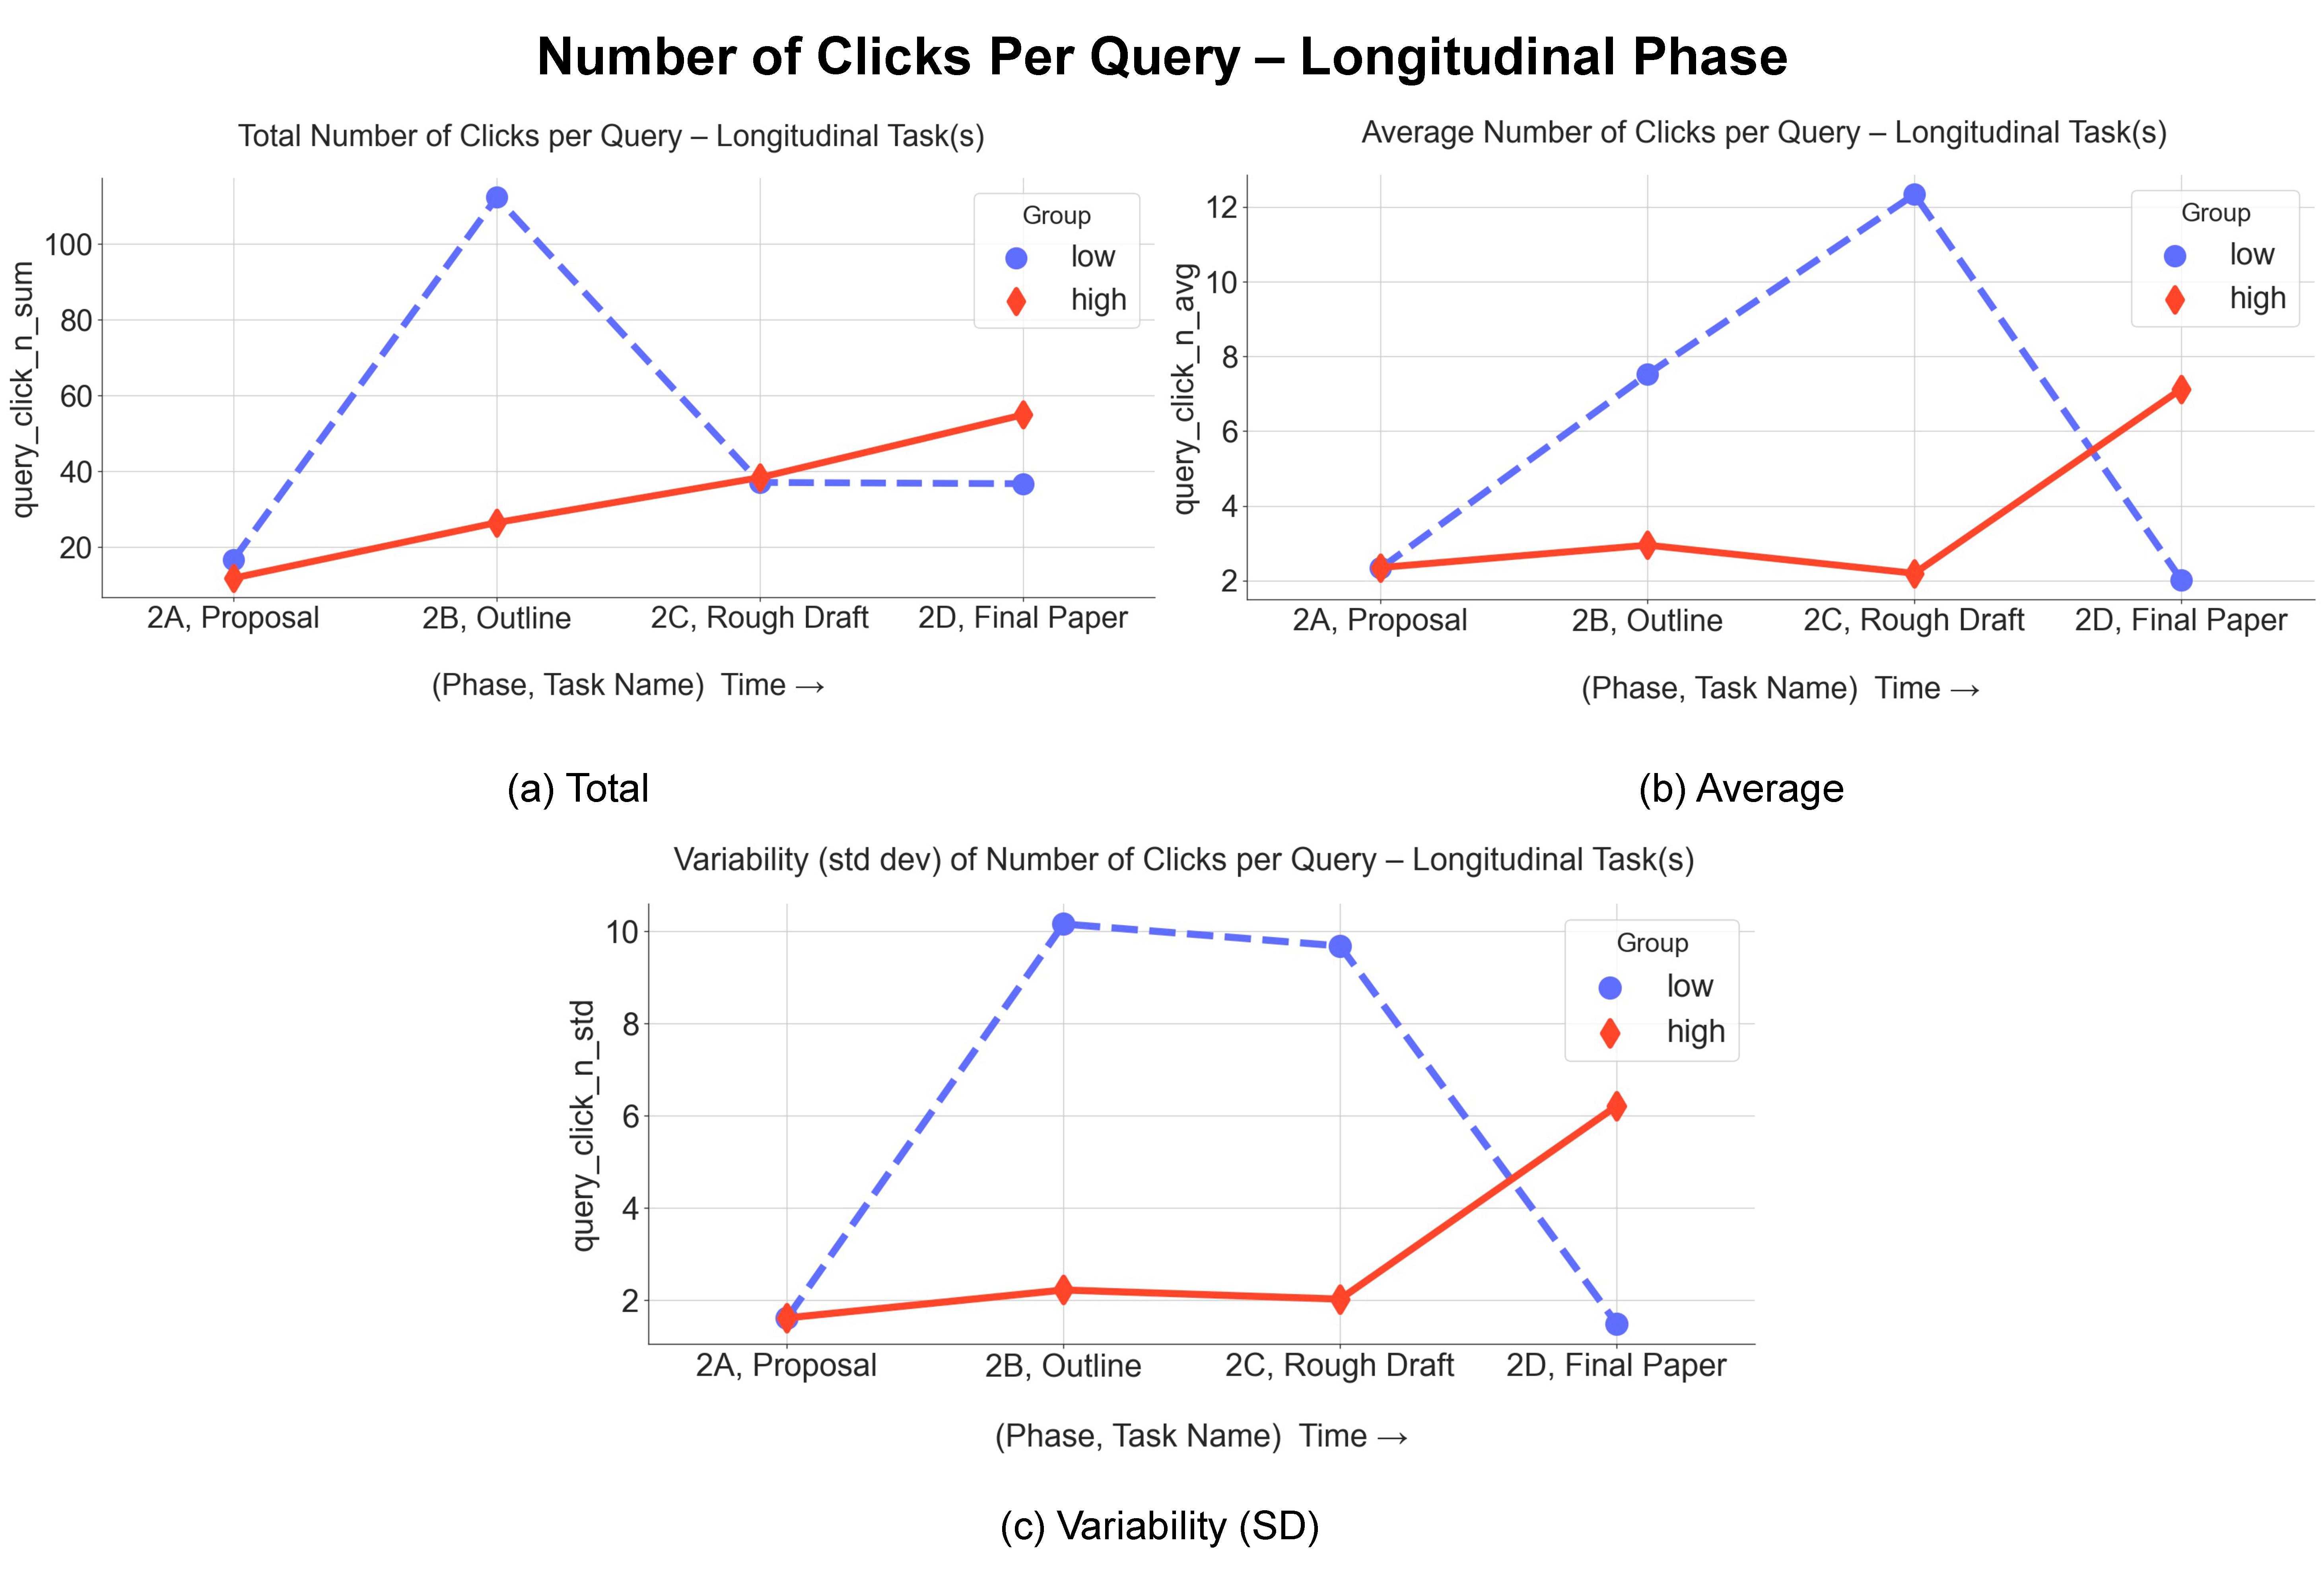
\includegraphics[width=1\linewidth]{figs/rp2-query-click} 

}

\caption[Number of clicks per query - longitudinal phase.]{Number of clicks per query - longitudinal phase.}\label{fig:rp2-query-click}
\end{figure}





Number of clicks per query refers to the number of times a participant clicked a link on a search result page after conducting a search query.
This metric reflects the level of interaction and engagement of the participant with the search results, as well as their ability to assess the relevance and usefulness of each search result presented to them.
A higher value of clicks per query may indicate that the participant is more engaged and willing to explore a wider range of information sources, while a lower value may suggest a more focused and targeted search approach.
Figure \ref{fig:rp2-query-click} shows the trend in total, average, and variability of clicks per query for the low and high groups at different points in the semester.

The low group had much higher total (Figure \ref{fig:rp2-query-click}(a)) and average (Figure \ref{fig:rp2-query-click}(b)) count of clicks per query, than the high group, at all stages of the semester -- proposal, outline, and rough draft -- except the last stage: writing the final paper.
The highest total clicks per query was during the outline phase (about 100 clicks total), while the highest average clicks per query was during the rough draft phase (about 12 clicks per query on average).
The high group maintained a relatively stable clicks per query during the proposal, outline, and rough draft stages (less than four clicks per query), and had a peak value of 7 clicks per query during the final paper.
Additionally, the high group had lower variability (standard deviation) in their number of clicks per query, compared to the low group (Figure \ref{fig:rp2-query-click}(c)).

The low group's higher total, average, and standard deviation of clicks per query throughout most of the semester, except for the final paper stage, suggests that they may have been less efficient in their searching behaviours, requiring more clicks and potentially spending more time on each query.
The may have struggled to refine their search strategies, resulting in more clicks per query throughout the semester.
This could have contributed to their lower self-perceived learning and search outcomes.

In contrast, the high group's fewer clicks per query throughout most of the semester, except for the final paper stage, suggests that they may have been more efficient and effective in their searching behaviours, requiring fewer clicks and potentially finding more relevant information per query.
They may have been able to refine their search strategies and be more efficient during the semester, resulting in fewer clicks per query.
This indicates the high group's ability to better assess the relevance and usefulness of search results, and to use their knowledge and cognitive strategies more effectively during the search process.
This could have contributed to their higher self-perceived learning and search outcomes.
The peak value of clicks per query for the high group during the final paper stage suggests that they may have needed to invest more effort in finding the most relevant and useful information for their final paper.
However, even at this stage, their average number of clicks per query was still lower than the low group's peak value during the rough draft stage.

It is also possible that the differences in average clicks per query between the two groups during different phases of the semester reflect differences in the complexity or specificity of the information needed for the different tasks. For example, the paper outline phase may have required more broad and exploratory searches, while the final paper phase may have required more targeted and specific searches.

\hypertarget{sec-phase2-res-L-dt}{%
\subsection{Counts and Dwell Time on Search Results}\label{sec-phase2-res-L-dt}}

\begin{figure}

{\centering 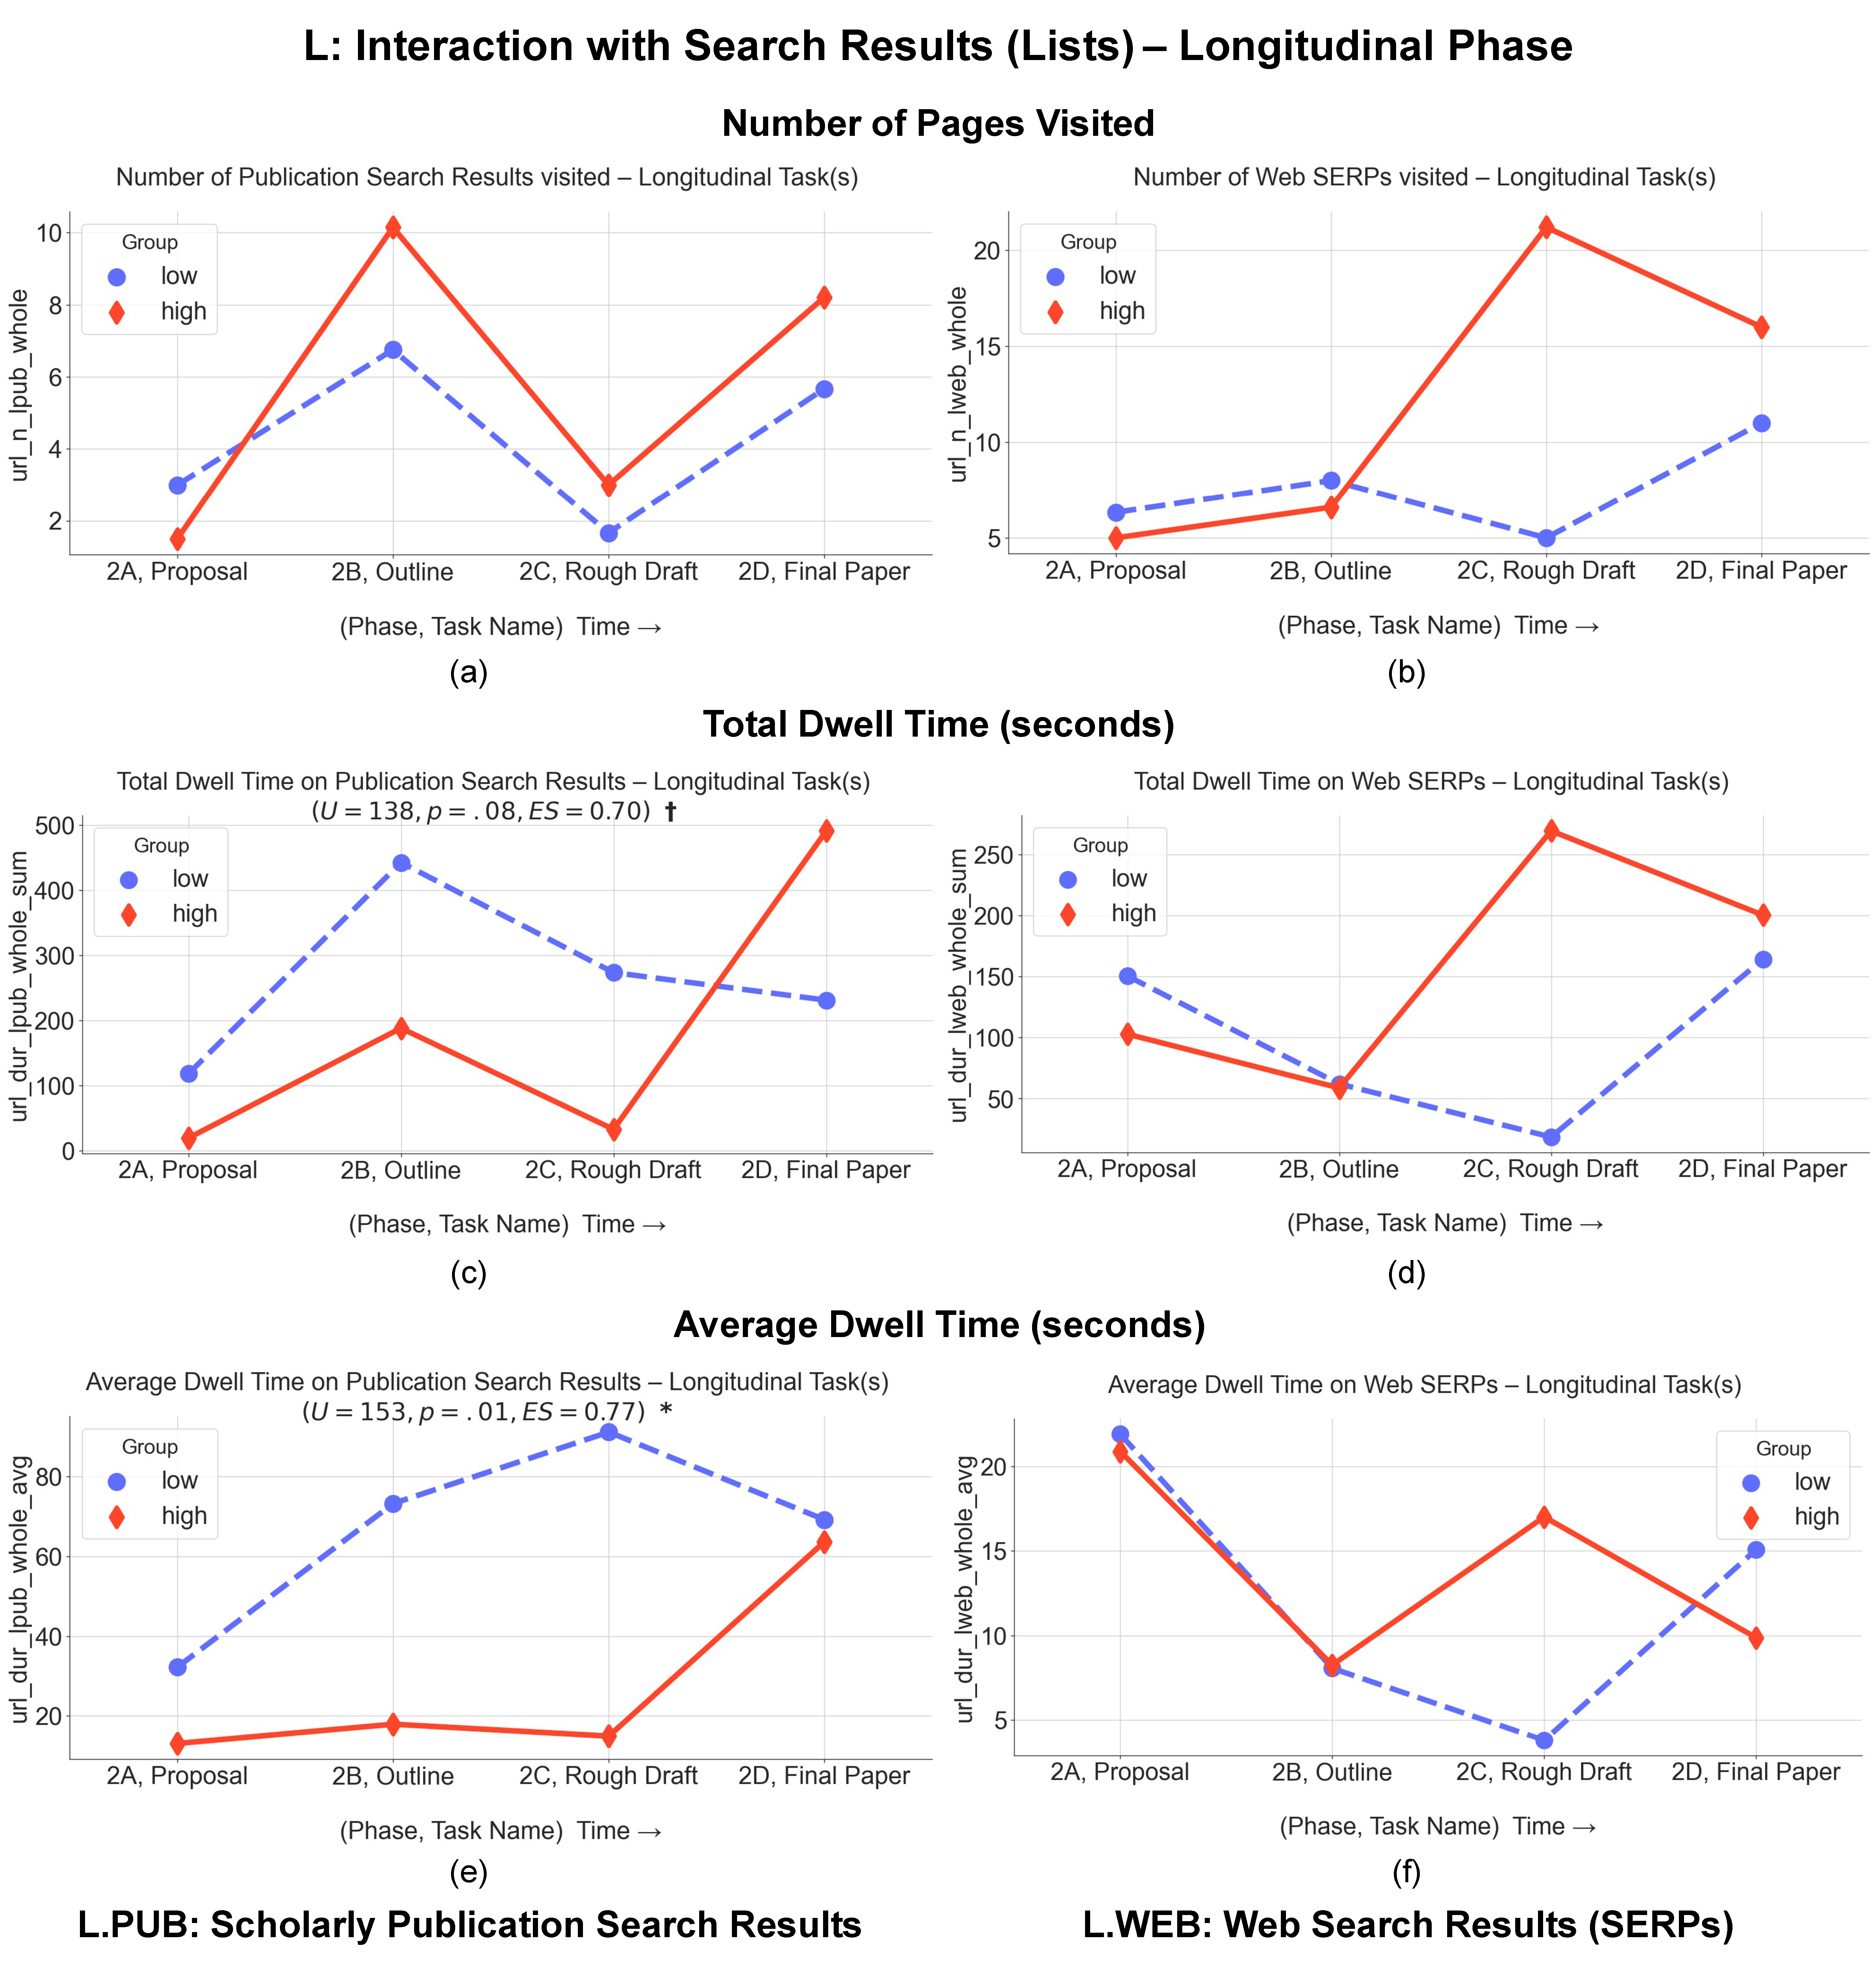
\includegraphics[width=1\linewidth]{figs/rp2-l} 

}

\caption[Interactions with search results - Longitudinal Phase.]{Interactions with search results - Longitudinal Phase.}\label{fig:rp2-l}
\end{figure}





The Ethical Dilemma research paper writing task involved searching for 20 references, and incorporating them into the narrative of the research paper.
Therefore, we structure the discussion around visits to scholarly publication search results, and (non-scholarly) web SERPs.
Examples of scholarly publication websites are Google Scholar, digital libraries such as ACM DL, Springer, Elsevier, PubMed and others.
We examined how visits to these two categories of websites changed across the different stages of writing the research paper for each group.
Figure \ref{fig:rp2-l} shows the counts of publication search results and web search results visited by the two groups, as well as total and average dwell time on such pages by both the groups.

For both publication search results and web search results, the high group visited more of those webpages than the low group (Figure \ref{fig:rp2-l}(a) and (b)).
The high group visited more publication search results during the outline phase, and more web SERPs during the rough draft phase.
The low group on the other hand, had a dip in their visit count for both the search result categories during the rough draft phase.
However, they had significantly longer average dwell time on academic publication search results, in all the four stages, compared to the high group \((U = 153.0, p = .01, ES = 0.77)\) (Figure \ref{fig:rp2-l}(e)).
Total dwell time of the low group was also longer, except at the final paper stage, when the high group surpassed the low group in dwelling on publication search results.
The difference was approaching significance \((U = 138.0, p = .08, ES = 0.70)\) (Figure \ref{fig:rp2-l}(c)).
This suggests that the low group spent more time examining and considering scholarly publication search results compared to the high group.
It is possible that the low group's lower levels of self-regulation and metacognition may have led them to spend more time on search results, as they may have found it harder to quickly evaluate and assess the relevance of search results to their task.
On the other hand, the high group's higher levels those individual traits may have enabled them to quickly identify relevant search results and move on to the next stage of their task.
However, at the final paper stage, the high group spent more time on search results as they may have needed to ensure that they had not missed any important information and had thoroughly covered their topic.

In general, the high group engaged more with web search results, and less with scholarly publication search results.
The low group demonstrated the opposite pattern.
This is an interesting finding.
The high group may have relied more on web search engines and popular sources, such as news articles or blogs, to get a broader understanding of their research topic and its context.
In contrast, the low group may have relied more on scholarly publications to find more in-depth and specialized information.
They may have been more thorough in searching for and evaluating academic publications, which was arguably one of the main aspects of writing the research paper.
This difference in strategy may have contributed to the difference in perceived learning outcomes between the two groups.
The high group may have been able to find a broader range of information from a variety of sources, while the low group may have limited themselves to more specialized sources.
It is also possible that the high group's use of web search engines may have resulted in them encountering more diverse perspectives and interpretations of the research topic, which could have enhanced their critical thinking and analytical skills.

\hypertarget{i-interaction-with-information-objects-sources-content-pages}{%
\section{I: Interaction with Information Objects -- Sources / Content Pages}\label{i-interaction-with-information-objects-sources-content-pages}}

\begin{figure}

{\centering 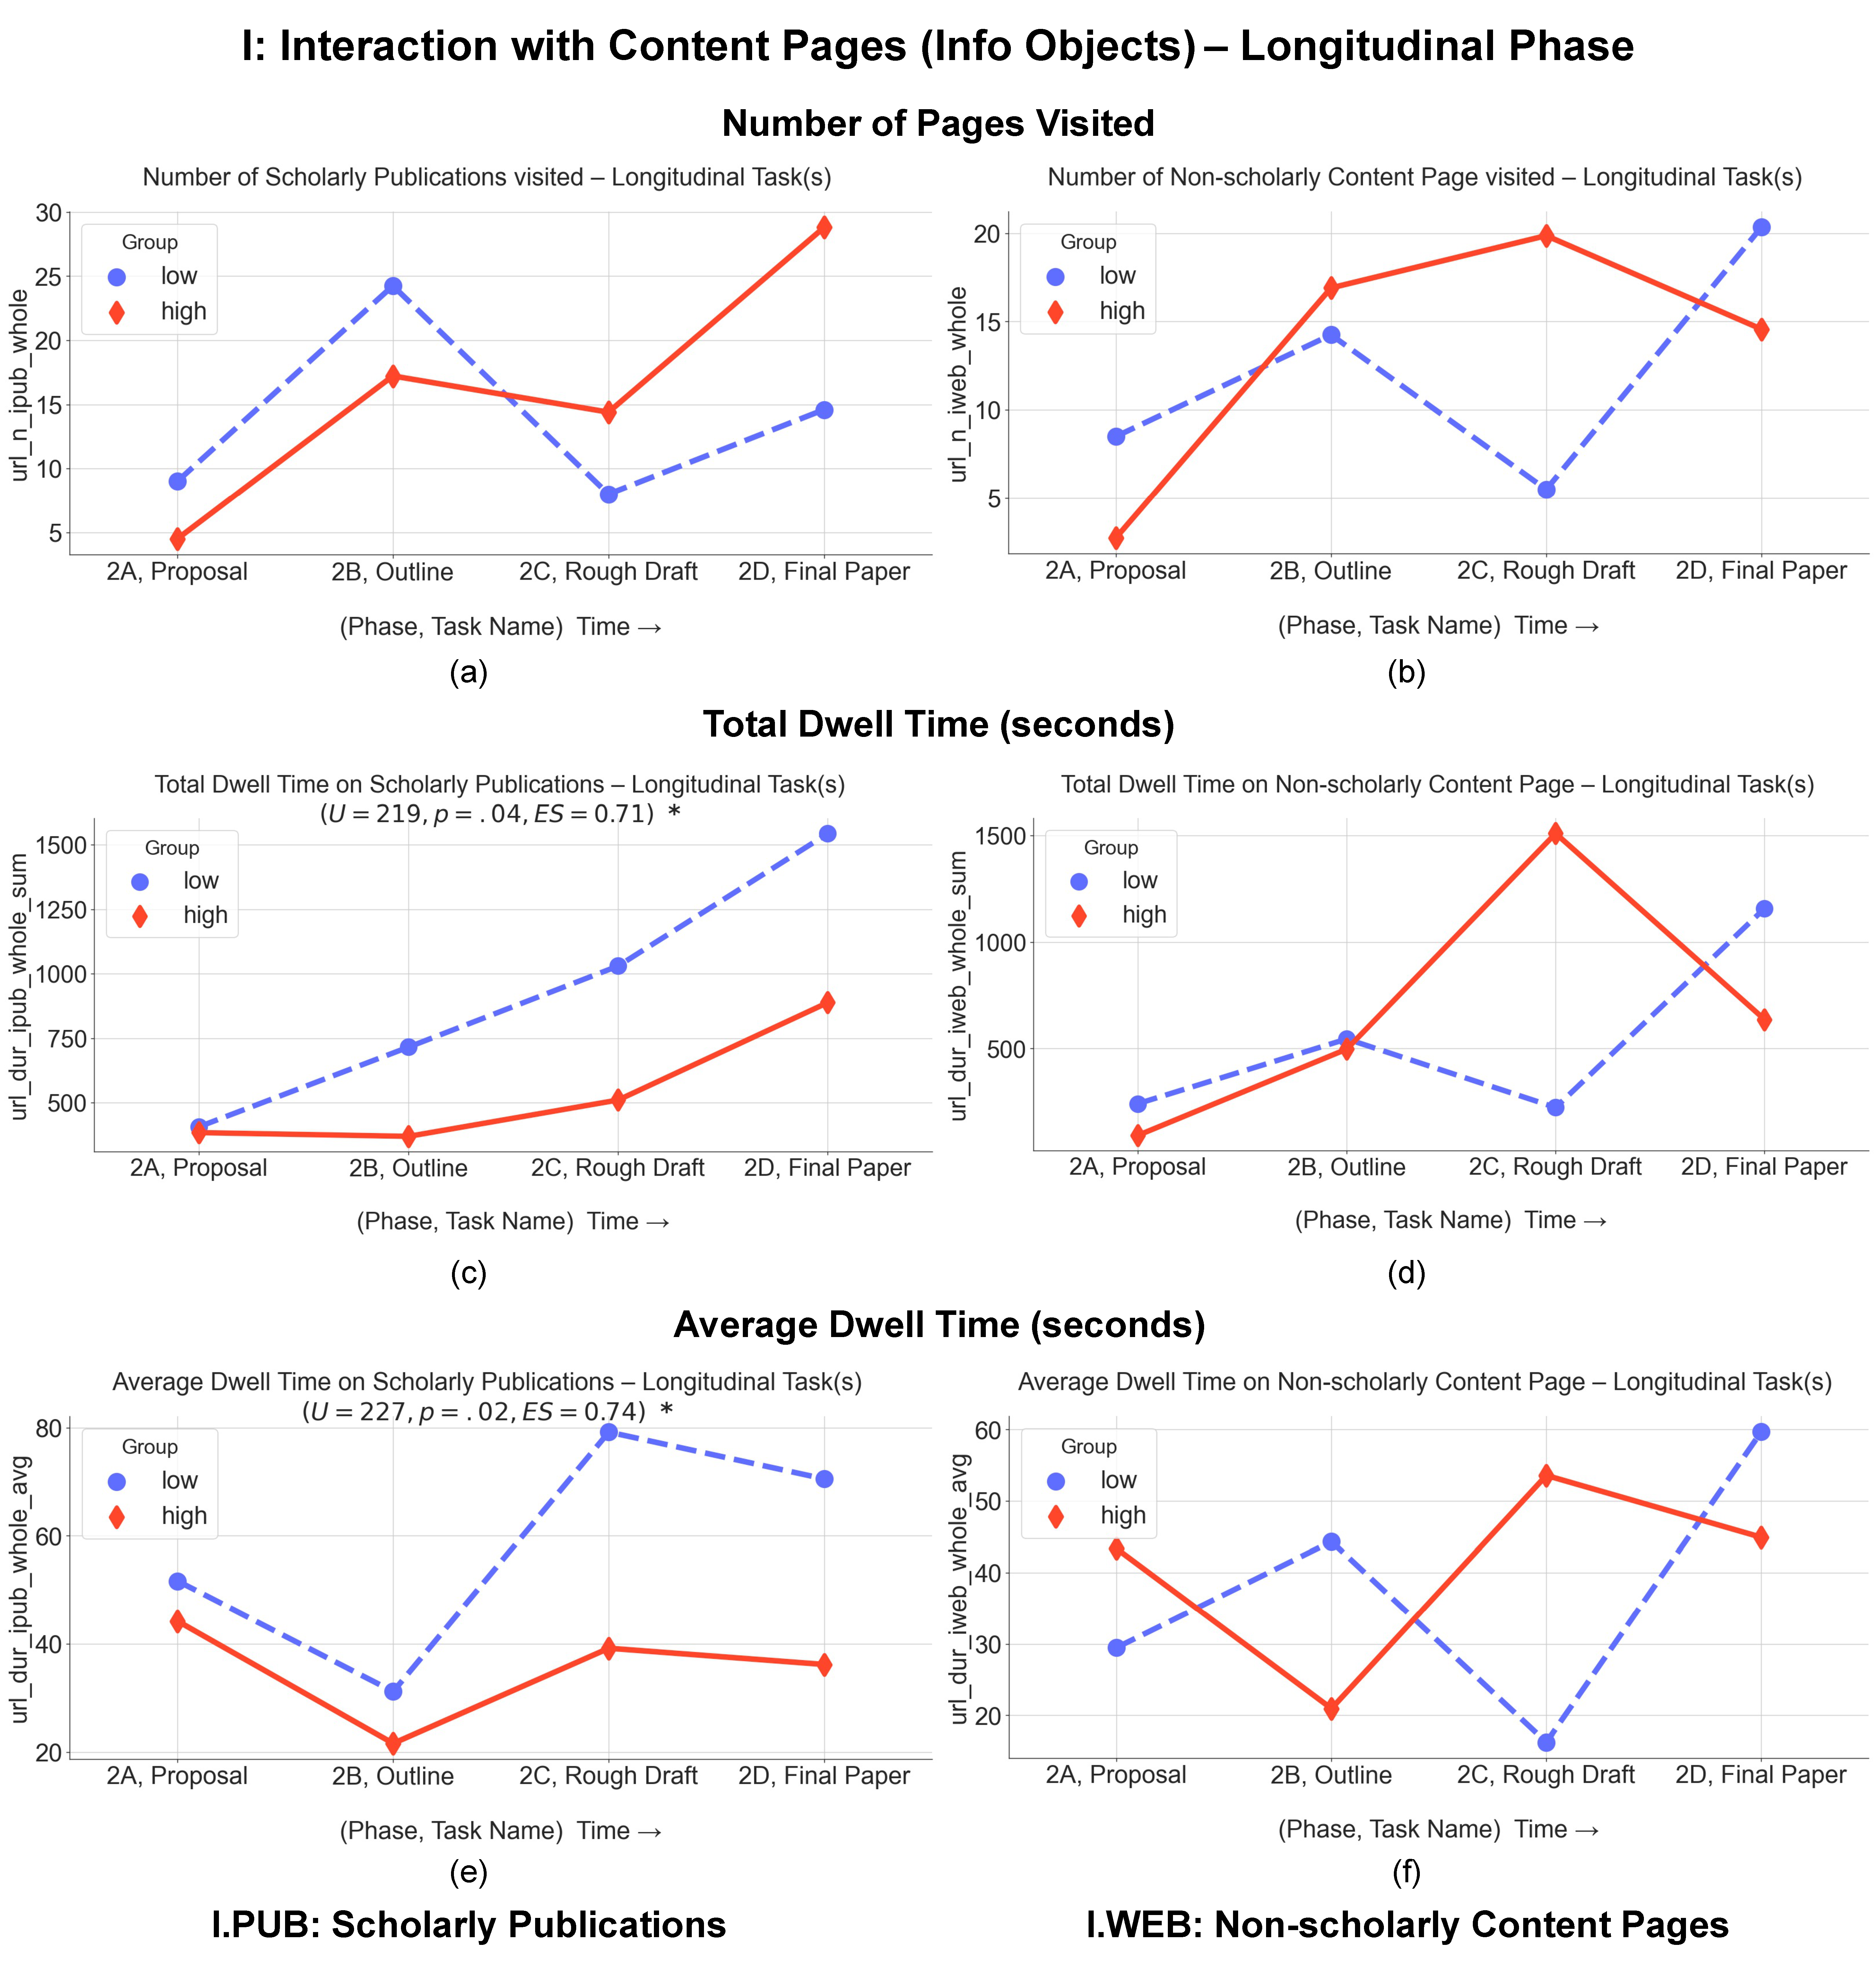
\includegraphics[width=1\linewidth]{figs/rp2-i} 

}

\caption[Interactions with content pages - Longitudinal Phase.]{Interactions with content pages - Longitudinal Phase.}\label{fig:rp2-i}
\end{figure}





We analysed interactions with content page in the same manner as counts and dwell time on search results (Section \ref{sec-phase2-res-L-dt}): looking at visits to scholarly publications, vs visits to non-scholarly content pages.
Figure \ref{fig:rp2-i} shows the counts of scholarly publications and non-scholarly content pages visited by the low and high groups, as well as total and average dwell time on such pages by both groups.

In a similar vein to publication vs web search results (Section \ref{sec-phase2-res-L-dt}), the high group engaged less with scholarly publications, and more with non-scholarly content pages, compared to the low group.
Earlier in the semester, while writing the outline, the low group visited more academic publications, while the high group visited more content pages.
The trend reversed later in the semester while writing the final paper, when the low group viewed fewer publications and more content pages, while the high group did the opposite (Figures \ref{fig:rp2-i}(a) and (b)).

Speaking of dwell times, the low group spent significantly more time viewing academic publications, in total \((U = 219.0, p = .04, ES = 0.71)\) and on average \((U = 227.0, p = .02, ES = 0.74)\), compared to the high group (Figures \ref{fig:rp2-i}(c) and (e)).
While writing the rough draft, the high group spent more time viewing non-scholarly content pages.

The high group's preference for non-academic content pages may reflect their use of web search engines to find relevant information, as such search engines may often prioritize non-academic content over scholarly publications.
The high group seemed to be more focused on finding information that was relevant to their topic, regardless of its source. They also appeared to be more interested in exploring a wider range of topics and concepts, which is reflected in their higher stationary entropy of query reformulations during the rough draft phase.

On the other hand, the low group's preference for academic publications may reflect their reliance on scholarly publication search engines to find information, as they may have perceived that being the main ask of the research paper.
The low group seemed to be more concerned with finding information from scholarly publications, perhaps as a way to demonstrate the rigour of their research.
They also appeared to have a more limited scope of inquiry, as reflected in their lower stationary entropy of query reformulations during the rough draft phase.

Overall, these findings suggest that the high group may have been more creative and adaptable in their information searching behaviours, while the low group may have been more rigid and focused on adhering to traditional academic norms.

\hypertarget{search-result-pages-vs-content-pages}{%
\section{Search Result Pages vs Content Pages}\label{search-result-pages-vs-content-pages}}

\begin{figure}

{\centering 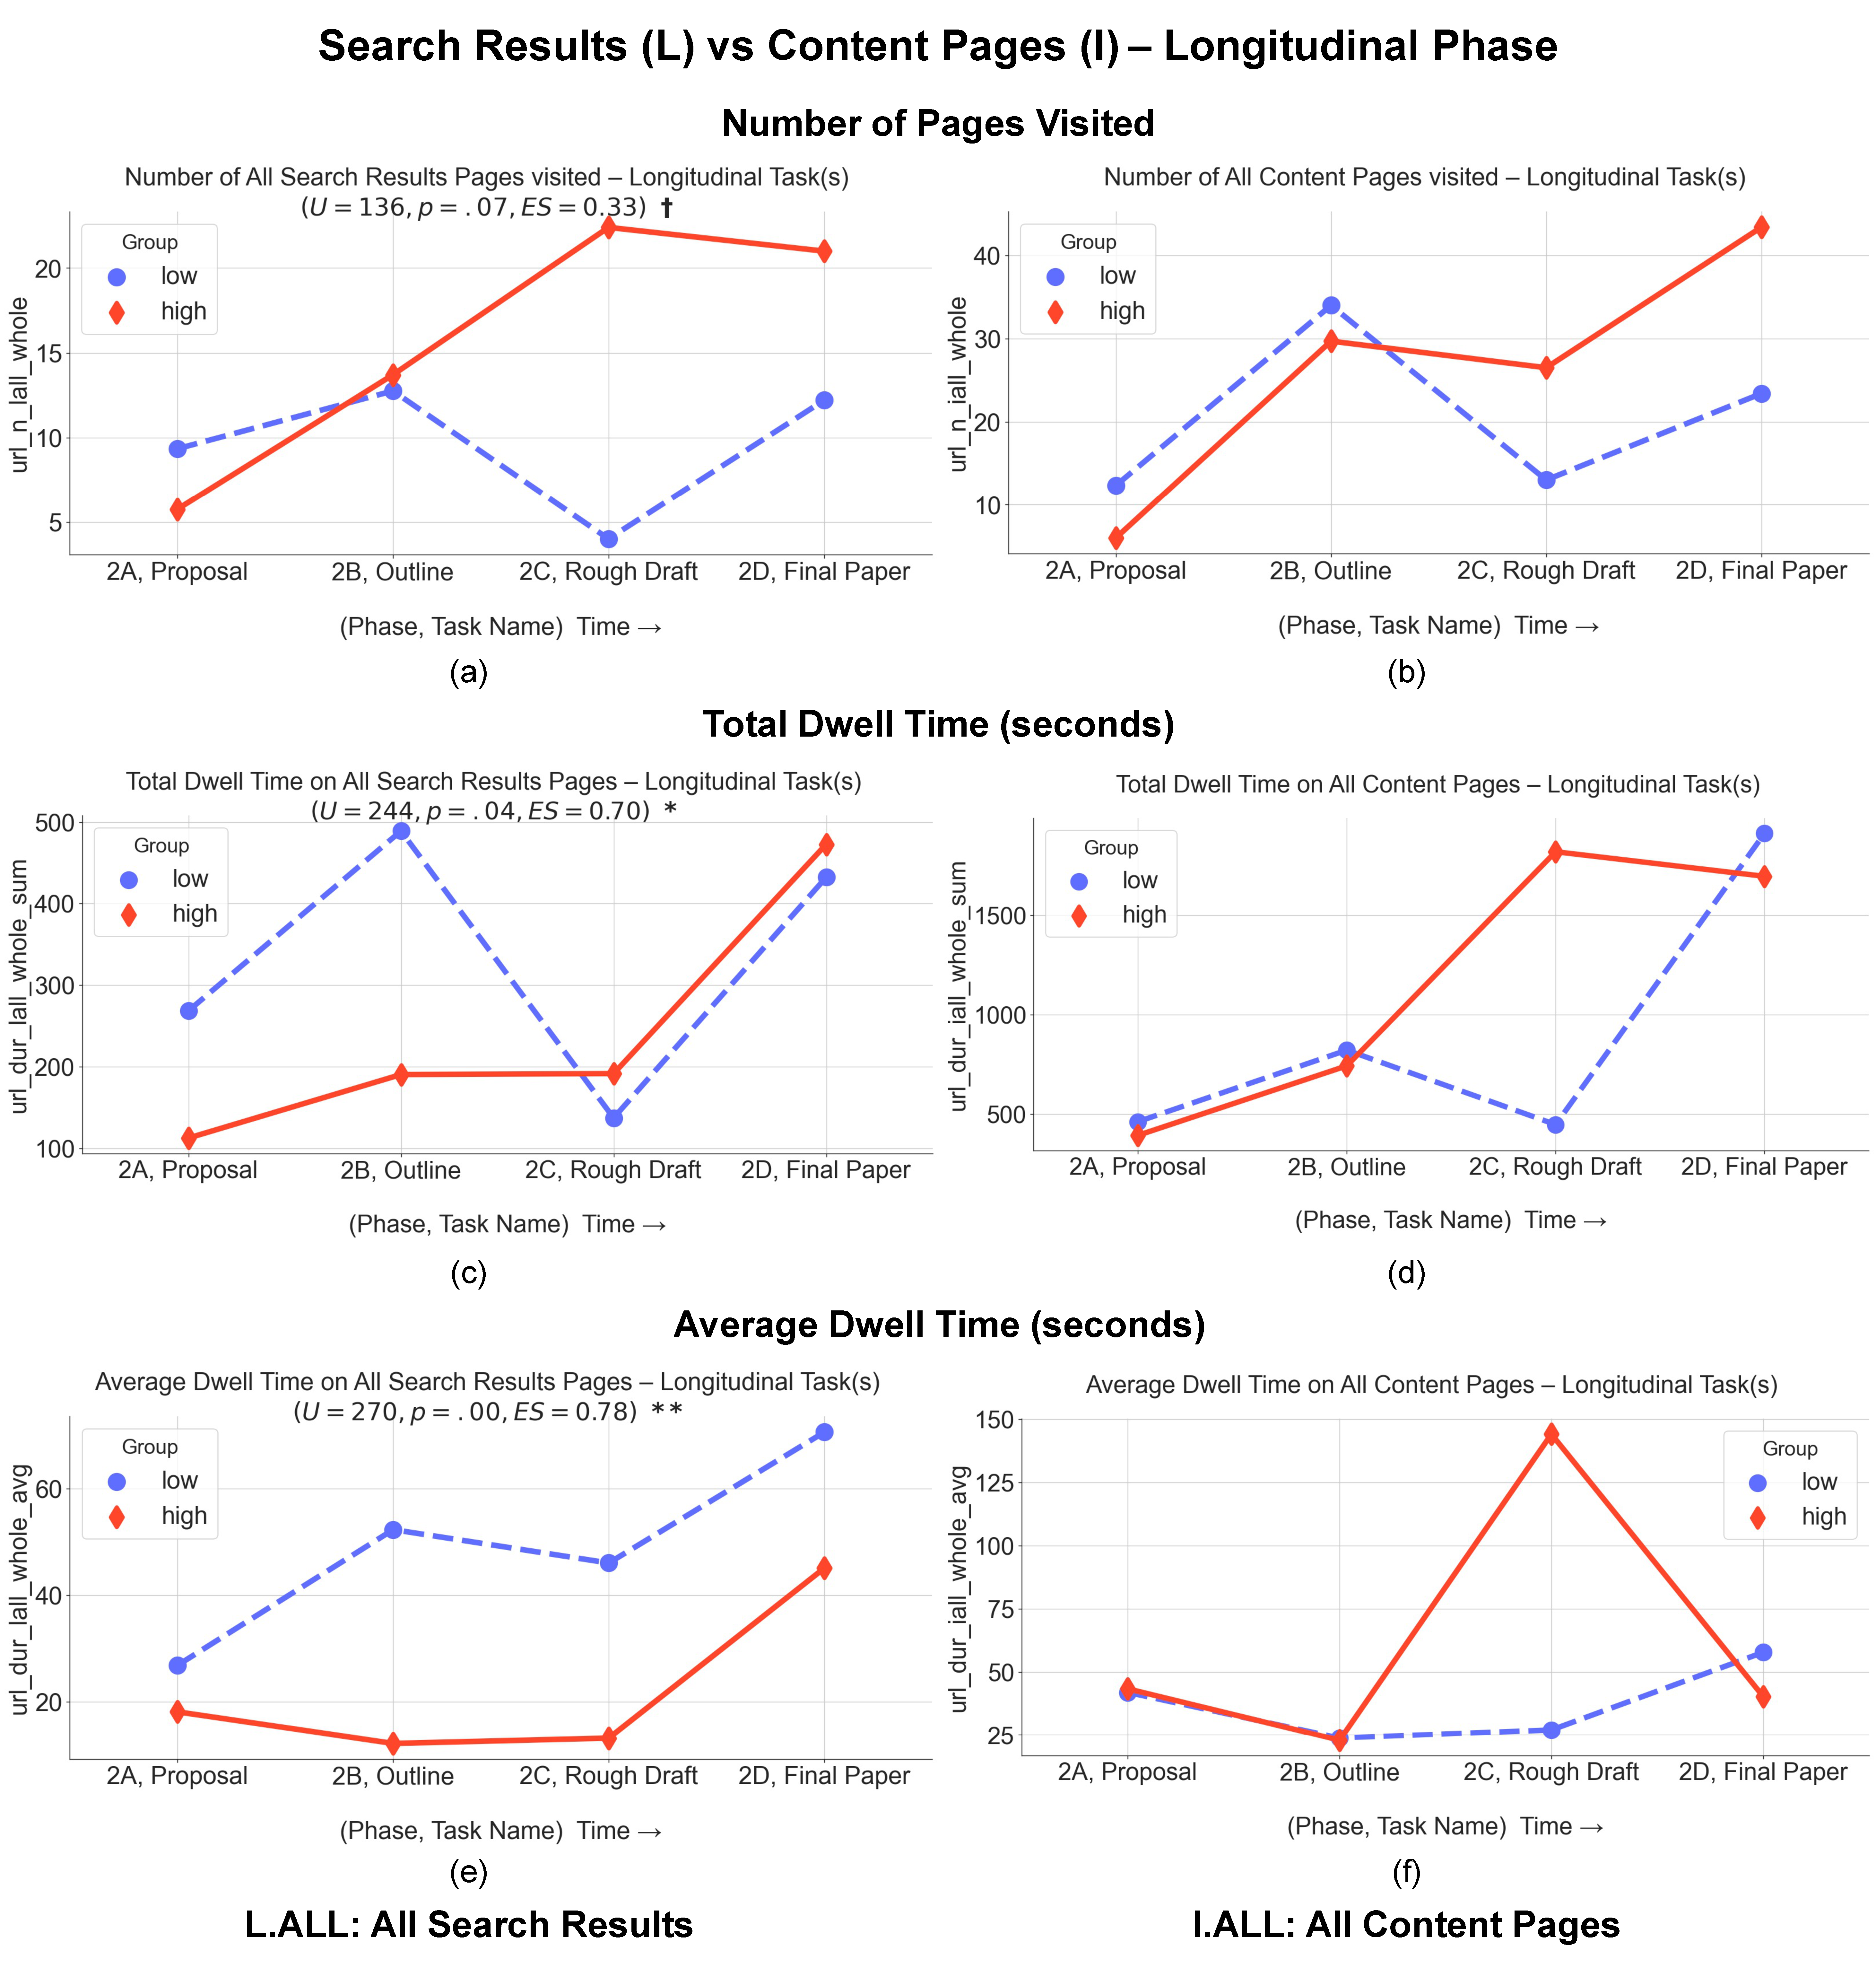
\includegraphics[width=1\linewidth]{figs/rp2-lvi} 

}

\caption[Differences in interactions with search results vs.~content pages - longitudinal phase.]{Differences in interactions with search results vs.~content pages.}\label{fig:rp2-lvi}
\end{figure}





Figure \ref{fig:rp2-lvi} describes differences in visits to all search results pages versus all content pages (scholarly and non-scholarly combined), for the high and low groups.
The high group visited more search result pages and content pages as the semester progressed, while the low group had a drop in these visits after the outline phase (Figure \ref{fig:rp2-lvi} (a), (b)).
The difference in the count of Search Results pages visited was almost significant \((U = 136, p = .07, ES = 0.33)\).
This suggests that the high group may have been more engaged and persistent in their information searching behaviours, while the low group may have experienced a decrease in motivation or self-regulation as the semester progressed, specifically before writing the rough draft.
It is also noteworthy that the low group had a rebound in the count of pages visited while writing the final paper. This could indicate that they were able to re-engage with the task, and their information searching behaviours improved as the final-paper deadline approached.

However, although the high group visited more webpages in general, they dwelt less on search results, and more on content pages.
The differences are significant for total and average dwell times on search results (Figure \ref{fig:rp2-lvi} (c) and (e)).
This indicates that the high group was more efficient at evaluating search result pages and quickly identifying relevant content.
On the other hand, the low group may have spent more time on search result pages, possibly indicating that they had a more challenging time evaluating and selecting relevant results.
For instance, when asked when if the participant had an experience where initially they thought they had found a useful resource, but upon later examination, they found it almost useless, a participant in the high group said:

\begin{quote}
\emph{I don't think so. I feel like I used all the papers that I found in my outline in my final paper, like some sort of degree.}

\hfill --- P023\_LONDON
\end{quote}

Another participant said:

\begin{quote}
\emph{I did find some articles that weren't useful, but I think I kind of quickly ruled them out all I'm looking like, from the title, they looked okay. Or sometimes even from the title, I just, like, didn't even look at them. But if I like looked at them a little bit closer and just clicked into them. And I didn't really find what they were saying very useful. Like, even in the introduction, I would just click out of them.}

\hfill --- P012\_MIAMI
\end{quote}

The above quotes illustrate the high group's efficiency at evaluating search result pages and quickly identifying relevant content. On the other hand, a participant in the low group described their struggle to identify relevant sources as follows:

\begin{quote}
\emph{Yes. Quite a lot, actually. A lot of them, like I saw Google highlights certain parts of the paper where it has the key words that I put in, and then I read about it. And it only briefly mentioned about that word or a couple of times. The distributed justice part, there's quite a lot. There's a lot of papers that has distributive justice in it. And then it's not really relevant. It just talks about distributive justice. Overall, it doesn't talk about distributive justice, as in terms of event, ensuring privacy. So it was pretty irrelevant.}

\hfill --- P007\_PARIS
\end{quote}

Thus, these differences in information behaviour could be related to the higher self-perceived learning outcomes and search outcomes seen in the high group, as they were able to find and engage with relevant content efficiently.

\hypertarget{entropy-of-search-tactic-sequences}{%
\section{Entropy of Search Tactic Sequences}\label{entropy-of-search-tactic-sequences}}

\begin{figure}

{\centering 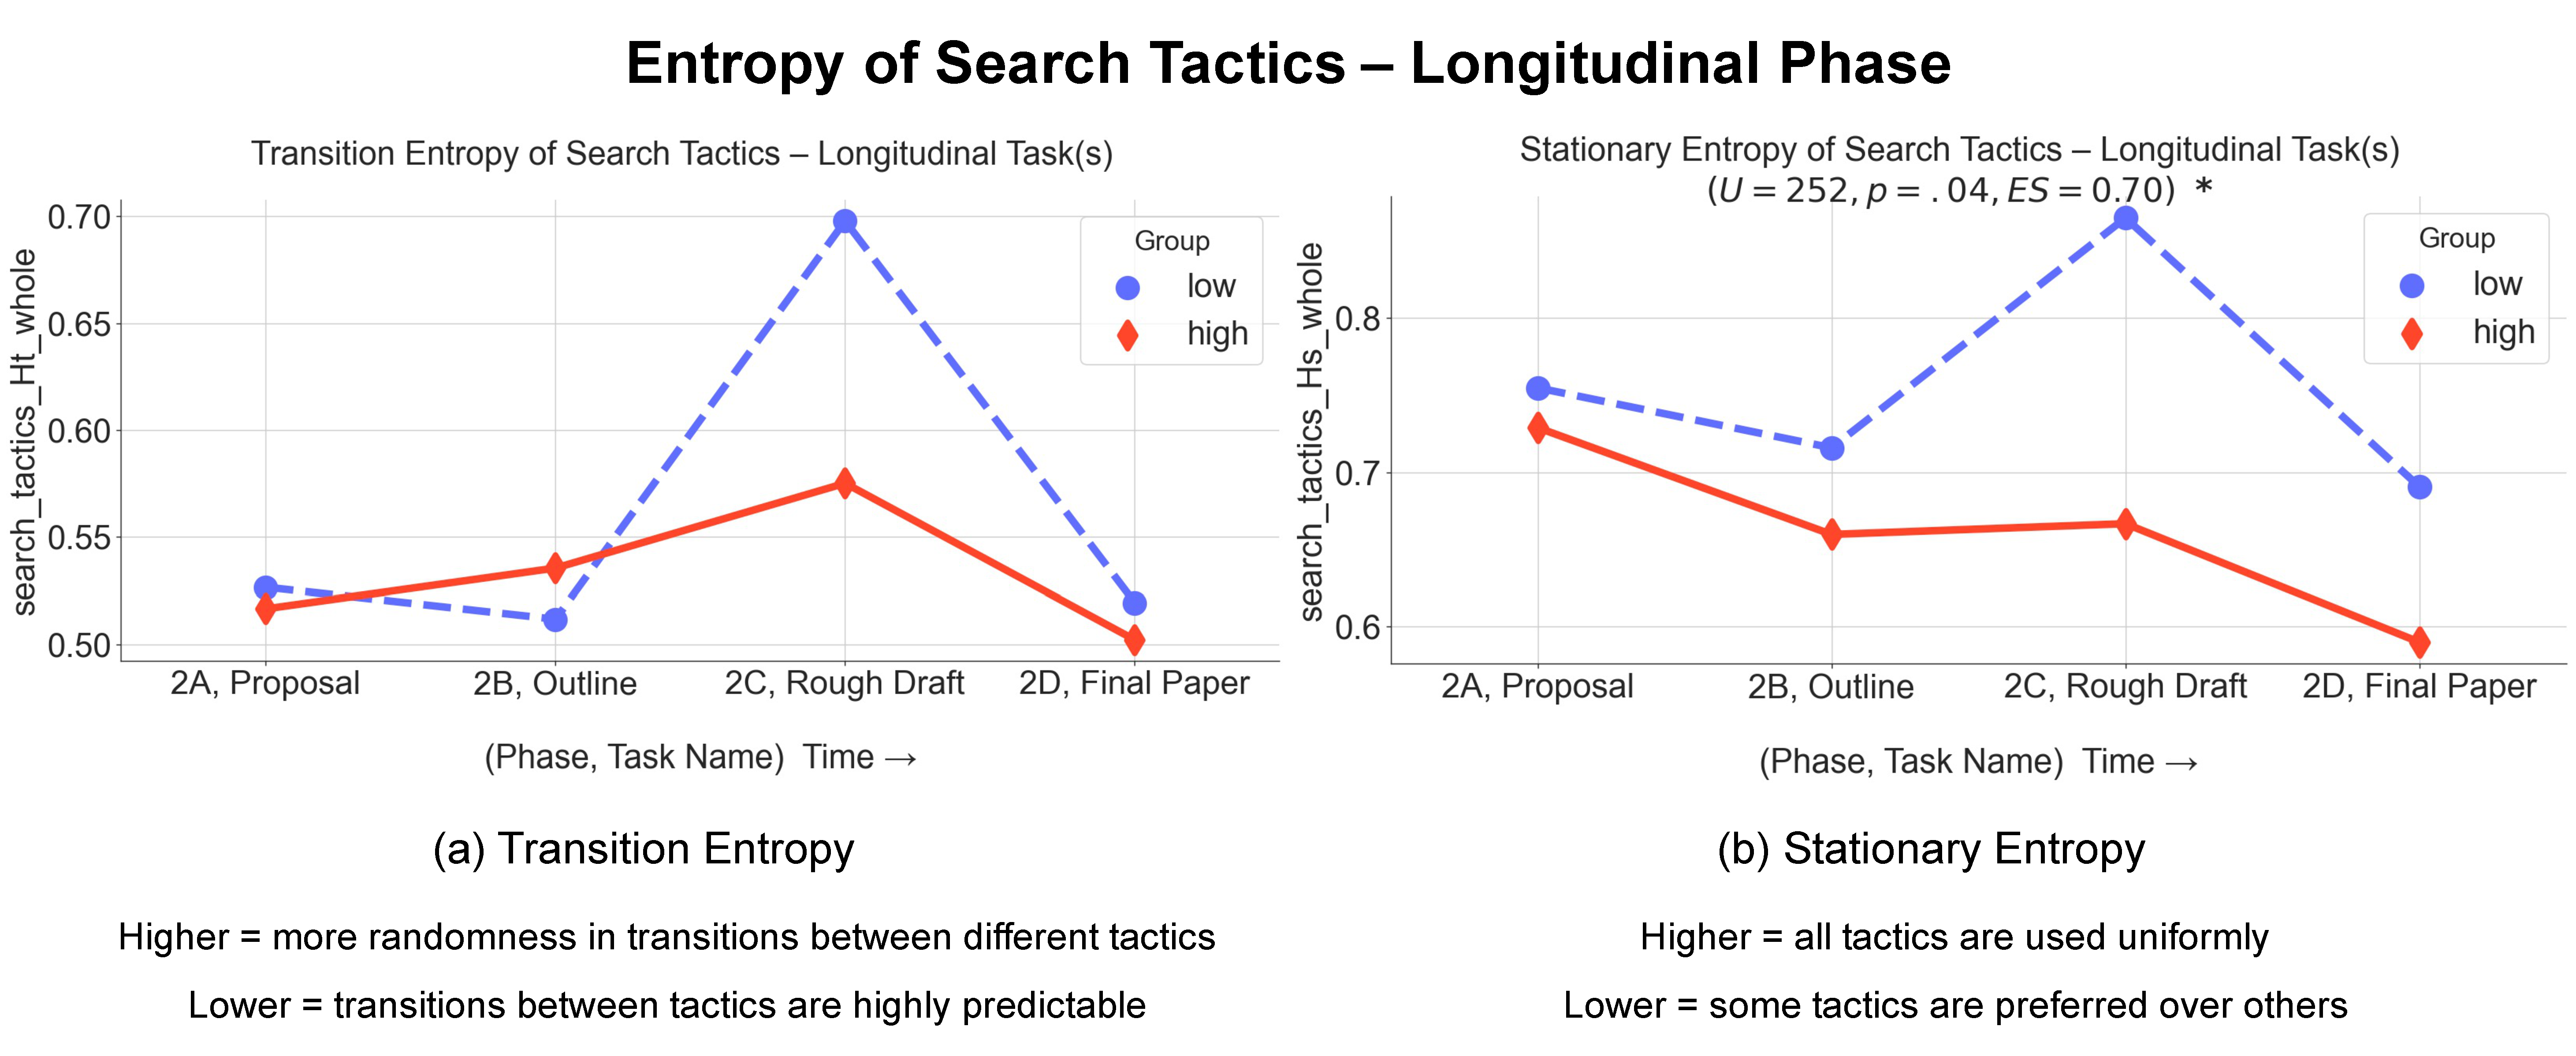
\includegraphics[width=1\linewidth]{figs/rp2-tactic-entropy} 

}

\caption[Entropy of search tactic sequences for longitudinal phase.]{Entropy of search tactic sequences for longitudinal phase.}\label{fig:rp2-tactic-entropy}
\end{figure}





Similar to entropy analysis of Query Reformulation types (Section \ref{sec-res-phase2-query-H}), we performed entropy analysis of search tactic transitions.
This analysis is directly inspired from He et al. (\protect\hyperlink{ref-he2016beyond}{2016}), who in turn were inspired from Krejtz et al. (\protect\hyperlink{ref-krejtz2015gaze}{2015}).
To characterize the entropy of students' search tactics, we used the following set of states, or tactics:

\begin{enumerate}
\def\labelenumi{\arabic{enumi}.}
\tightlist
\item
  \textbf{\texttt{QUERY}}: issuing a search query
\item
  \textbf{\texttt{CLICK}}: mouse click
\item
  \textbf{\texttt{IDLE}}: participant stays idle for more than one minute (adapted from Taramigkou et al. (\protect\hyperlink{ref-taramigkou2018leveraging}{2018}))
\item
  \textbf{\texttt{SESSION\_BREAK}}: participant becomes idle for more than 30 minutes (Google Analytics defines a session break as 30 minutes of inactivity \footnote{\url{https://support.google.com/analytics/answer/2731565\#zippy=\%2Cin-this-article}})
\item
  \textbf{\texttt{L.PUB}}: visiting a publication search result page
\item
  \textbf{\texttt{L.WEB}}: visiting a web SERP
\item
  \textbf{\texttt{I.PUB}}: visiting a scholarly publication
\item
  \textbf{\texttt{I.WEB}}: visiting a non-scholarly content page
\item
  \textbf{\texttt{TASKPAGE}}: visiting webpages related to the study, i.e.~the Qualtrics questionnaires
\end{enumerate}

In the context of search tactic transitions, a higher value of transition entropy (\(H_t\)) indicates more randomness and uncertainty in the participant's search behaviour (which is composed of different search tactics, and transitioning or switching between those tactics).
A lower value of transition entropy indicates that the search behaviour (i.e.~tactic switching behaviour) is highly predictable.
For stationary entropy of search tactics (\(H_s\)), a higher value indicates that participants utilize all the search tactics with equal probability, while a lower value suggests that certain search tactics are favoured over others.
Figure \ref{fig:rp2-tactic-entropy} describes the trends in this values over the duration of the semester.

The low group demonstrated a sharp increase in both transition entropy and stationary entropy of search tactics from the proposal stage to the outline stage.
Both the entropies subsequently decreased in the final paper stage.
The high group had a relatively stable trend in their transition entropy of search tactics, while their stationary entropy decreased as the semester progressed.
Also, the high group's stationary entropy was significantly lower than that of the low group \((U = 252.0, p = .04, ES = 0.70)\).

The low group's sharp increase in both transition and stationary entropy from the proposal to the outline stage suggests that they were exploring a wider range of search tactics and were less certain of which tactics to use during the early stages of the writing process.
This is consistent with their high counts of query reformulations, and tendency to click on many search results and content pages.
The subsequent decrease in both entropies in the final paper stage suggests that the low group became more focused and efficient in their search tactics, possibly as a result of the feedback they received during the earlier stages of the writing process.

The high group's relatively stable trend in transition entropy suggests that they were consistent in their use of search tactics throughout the writing process.
However, their decreasing stationary entropy suggests that they became more focused and efficient in their use of search tactics as the semester progressed, which is consistent with fewer query reformulations, and tendency to dwell more on content pages.

The quantitative results from the entropy analyses also get supported by qualitative responses from the participants.
When asked if they had a plan before starting the project, or starting to search, a participant in the low group responded:

\begin{quote}
\emph{\textbf{Not really.} My plan was just to find sources and see how they kind of fit in with my research question. And \textbf{if I didn't really find anything, I would just alter the research question}.}

\hfill --- P012\_MIAMI
\end{quote}

In contrast, a participant in the high group responded:

\begin{quote}
\emph{whenever I start searching, \textbf{I go in with the mindset of: this is what I'm searching for}\ldots{} I always try to reference back to that main goal to help guide my searching process,\ldots{} like, Okay, I'm searching for content articles, right? And so \textbf{I'm not gonna go ahead and get distracted by anything else}, that's going to be like my main goal. And as long as I'm able to go ahead and reference that back to my main goal, then I'm doing a good job.}

\emph{I feel this is something that I've gotten used to being a college student. I realized, this is probably the most efficient way to search for things (and) \textbf{not get overwhelmed}. \textbf{Breaking it down and having a very clear set goal makes things more manageable for me}.}

\hfill --- P015\_LIMA
\end{quote}

Overall, these quantitative and qualitative differences in the two groups approached the research project suggest that the low group was more uncertain and exploratory in their search tactics, while the high group was more focused and efficient.

\hypertarget{summary-of-longitudinal-phase}{%
\section{Summary of Longitudinal Phase}\label{summary-of-longitudinal-phase}}

We summarise the findings from this chapter, on the longitudinal searching-as-learning task of writing a research paper, as follows.

Participants were divided into high and low groups based on their self-reported values of motivation, metacognition, self-regulation, and memory span.
Their search behaviour and perceived learning and search outcomes were studied over the course of a semester.
During the longitudinal phase, both the high and low groups exhibited changes and differences in their search behaviour from the proposal to the outline stage to the rough draft, and finally to the final paper stage.

Investigating into specific interaction patters, we saw that the high group visited more search result pages, but spent less time dwelling on them. They also visited more content pages in the later parts of the semester, and spent more time dwelling on them.
The low group visited fewer search result pages, but spent more time on evaluating search results.

Transition entropy refers to the uncertainty of the next search tactic that a user will apply during their search.
In other words, it is a measure of how much the user explores different search tactics over the course of their search.
Stationary entropy refers to the uncertainty of the search tactic distribution over time.
It is a measure of how stable or consistent the user is in their use of search tactics throughout their search process.
The low group showed sharp increases in both transition entropy and stationary entropy of search tactics from the proposal stage to the outline stage, followed by a decrease in both entropies in the final paper stage.
This indicates that their search tactics became more diverse and unpredictable in the middle stages of the task, possibly due to uncertainty and lack of clarity on the topic.
The high group had a relatively stable trend, or gentle increase in their transition entropy of search tactics, indicating that they had a consistent and well-defined search strategy.
This group's stationary entropy decreased as the semester progressed, suggesting that they became more focused and efficient in their search tactics over time.
Additionally, the high group's stationary entropy was significantly lower than that of the low group, indicating that they had a more structured and organized approach to their search tactics.

Regarding learning and search outcomes, the high group demonstrated significantly higher perceived learning and search outcomes compared to the low group.
Although the high group received slightly better grades on their research paper assignments, though there was no significant difference between the two groups.
Possibly, other factors beyond self-perceived searching and learning outcomes may have contributed to the overall grade.

\hypertarget{results-and-discussion-repeated-vs-non-repeated-search-tasks}{%
\chapter{Results and Discussion: Repeated vs Non-repeated Search Tasks}\label{results-and-discussion-repeated-vs-non-repeated-search-tasks}}

Apart from the longitudinal phase of the study discussed in the previous chapter, participants also completed two search tasks at the beginning of the semester (\texttt{PHASE1}), and two search tasks at the end of the semester (\texttt{PHASE3}).
One set of tasks, on the topic of ``personal finance for college students'', was repeated at the end of the semester (repeated search tasks).
The other set of tasks was not repeated (non-repeated search tasks), and the topics were ``ubuntu ethics'' in the beginning of the semester, and ``algorithmic bias'' at the end of the semester.
These topics for the non-repeated search tasks were selected from the content of the I303 course that the participants were enrolled in.

The initial and final phases of the study aimed to compare the information search behaviours of students across repeated and non-repeated search tasks, at the beginning and end of the semester.
This chapter presents the results of the analysis, which involved comparing the entropies of search tactics and query reformulation sequences, clicks per query, and interaction with different categories of webpages.
Let us now discuss some of the findings for these repeated versus non-repeated tasks
We use the same low-high groups from the LPA analysis discussed in Section \ref{sec-res-phase2-lpa}.

\hypertarget{learning-outcomes}{%
\section{Learning Outcomes}\label{learning-outcomes}}

\begin{figure}

{\centering 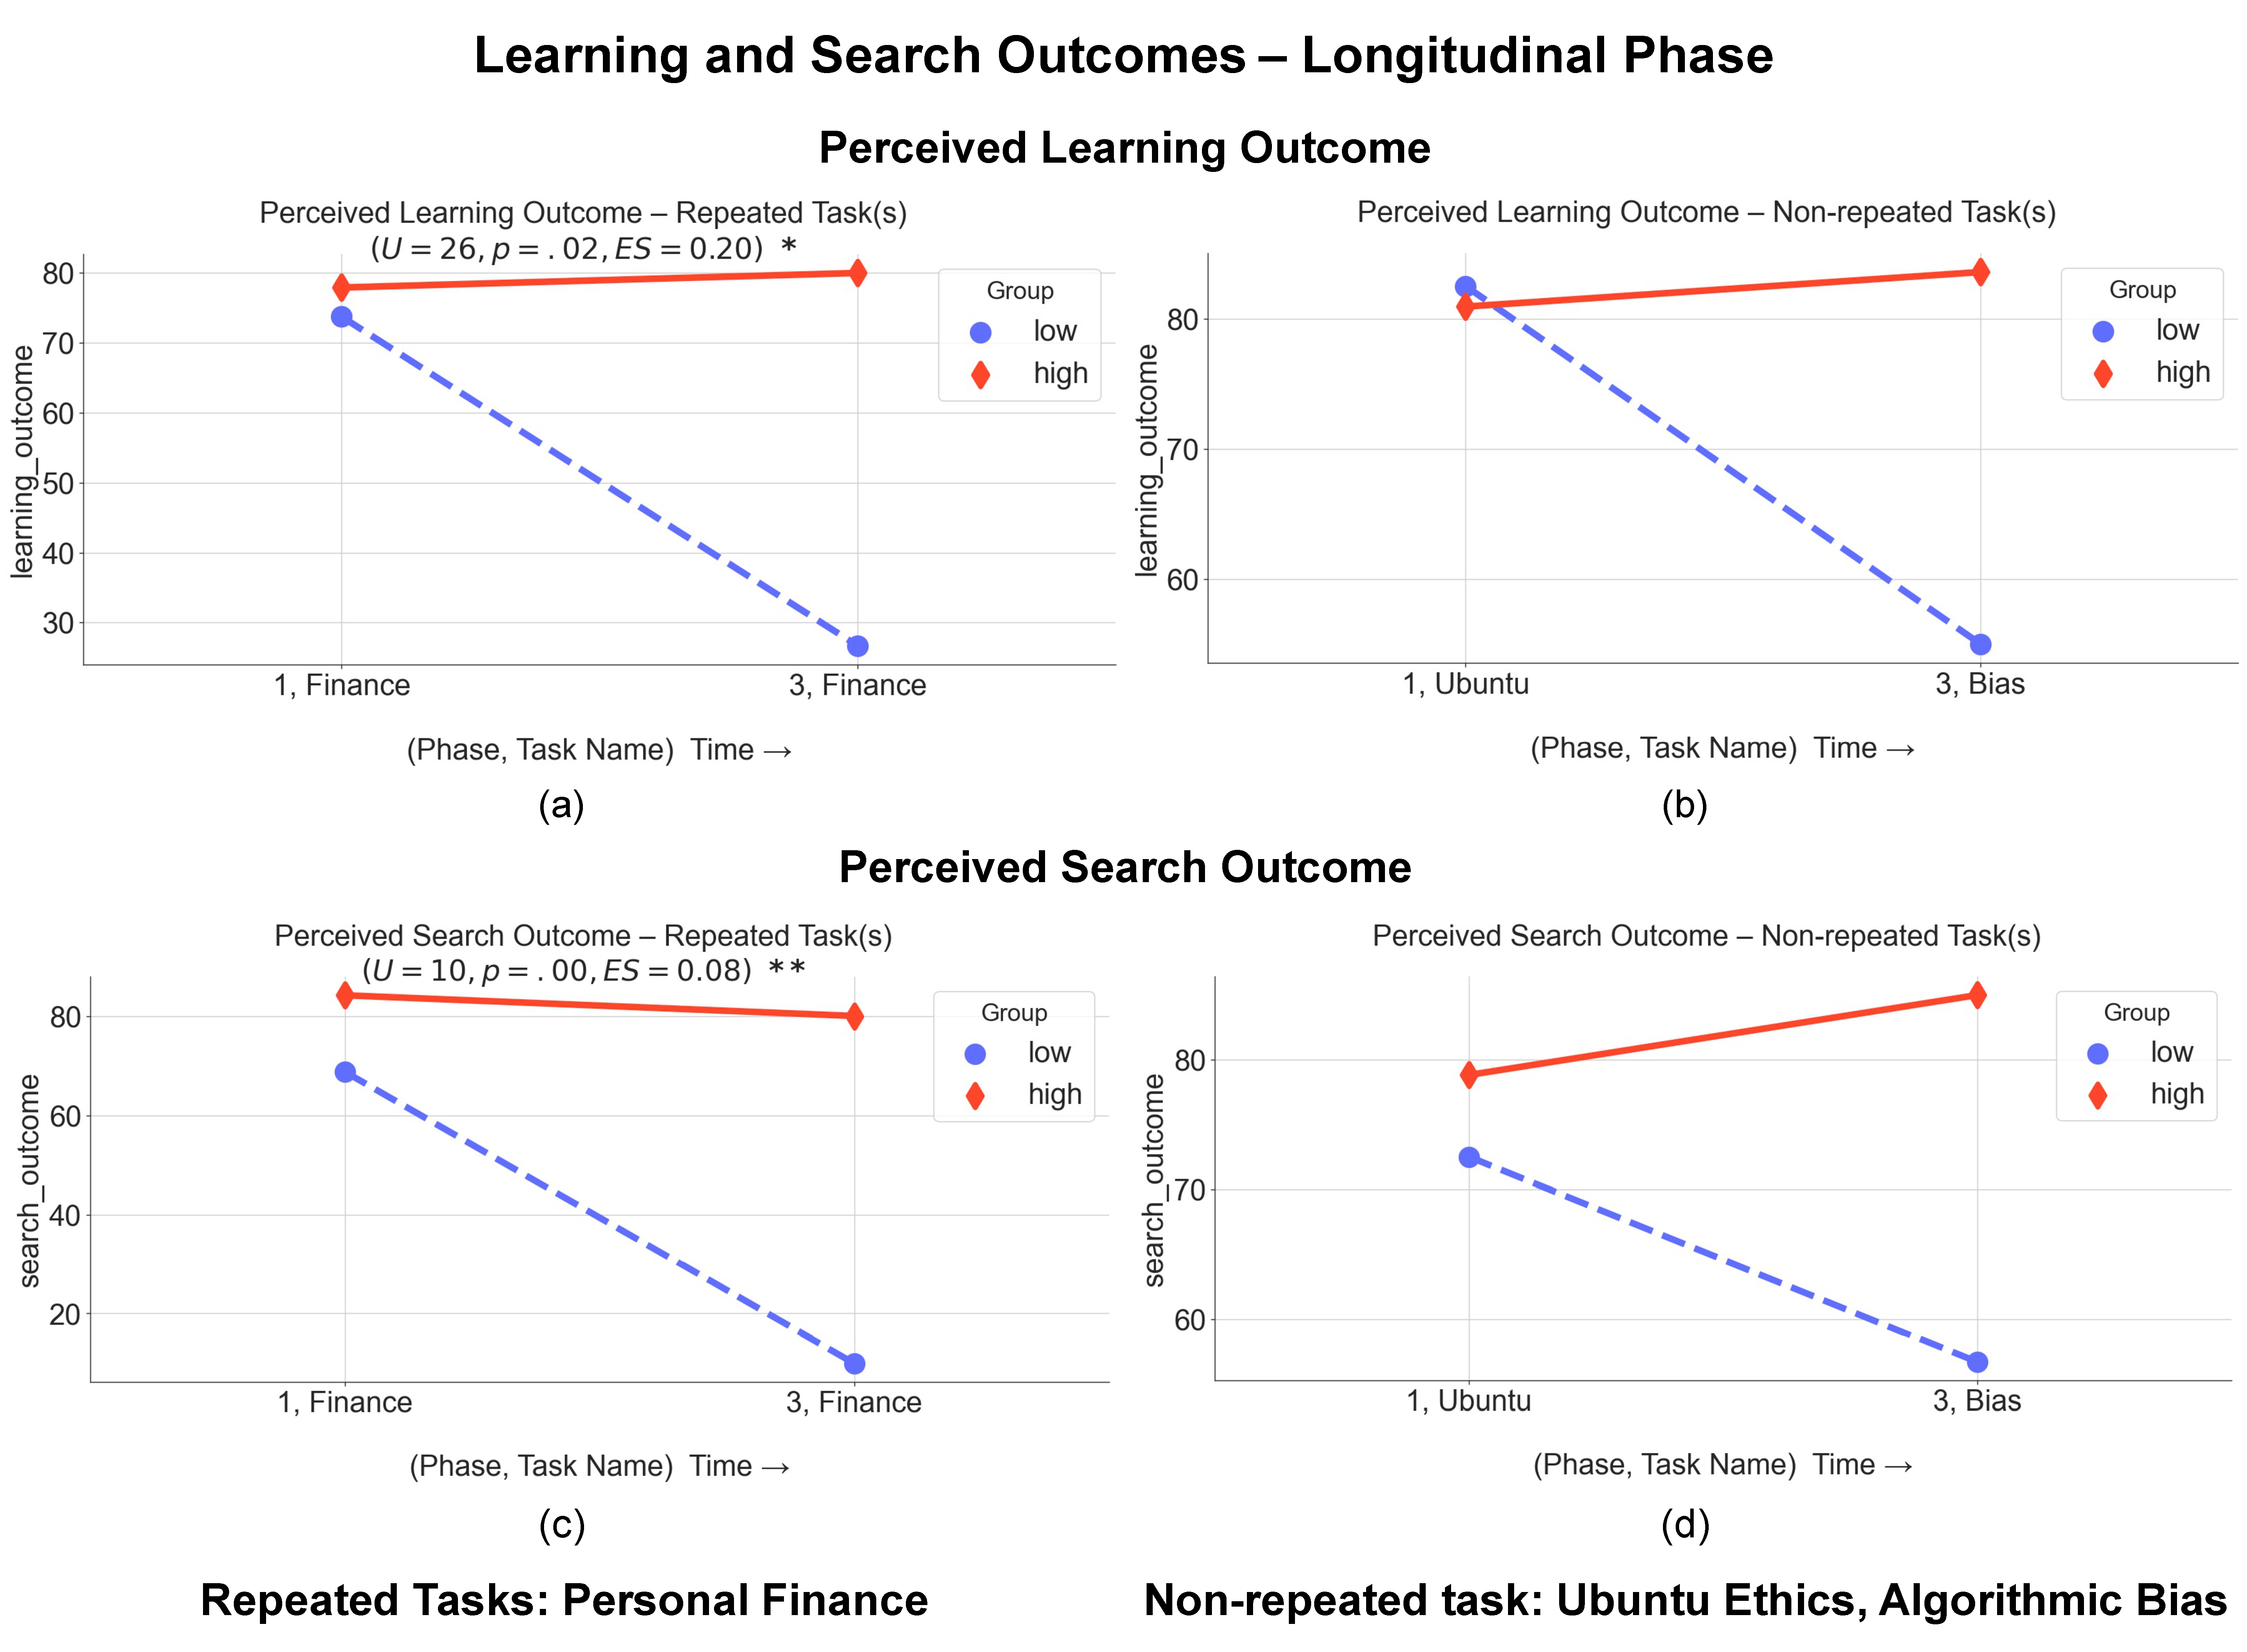
\includegraphics[width=1\linewidth]{figs/rp13-learning-search-outcomes} 

}

\caption[Learning and Search Outcomes -- Longitudinal Phase.]{Learning and Search Outcomes -- Longitudinal Phase.}\label{fig:rp13-learning-search-outcomes}
\end{figure}





Figure \ref{fig:rp13-learning-search-outcomes} shows the differences in perceived learning outcomes and perceived search outcomes for the two sets of tasks for the low and high groups.
The high group reported higher learning and search outcomes for both repeated and non-repeated tasks, at both the beginning and the end of the semester.
For the low group, their perceived learning and search outcomes decreased for all the tasks at the end of the semester.
The differences between the groups were statistically significant for the repeated task (on the topic of Personal Finance) -- \((U = 26.5, p = .02, ES = 0.20)\) for perceived learning outcome, and \((U = 10.5, p = .001, ES = 0.08)\) for perceived search outcome.

There could be several factors contributing to the differences in perceived learning and search outcomes between the two groups.
One possible explanation is that the high group had better information-seeking strategies and habits that allowed them to more effectively find and evaluate relevant information, leading to higher perceived learning outcomes. As discussed in the longitudinal phase findings, the high group engaged more with web search results and content pages, while also spending less time on search results and academic publications. This suggests that they were able to efficiently navigate through search results and find the most relevant information.
Another possible explanation is that the high group had better prior knowledge and familiarity with the topics, which allowed them to more quickly and effectively identify relevant information.
Additionally, it is possible that the high group had more motivation and interest in the topics, leading to more engagement and effort in the search process, and ultimately higher perceived learning outcomes.

For the low group, the decrease in perceived learning and search outcomes at the end of the semester could be due to a variety of factors, such as burnout or fatigue from the research paper writing process, or a lack of engagement or motivation. The decrease in their search tactics entropy and dwell time on academic publications and search results over the course of the semester suggests that they may have become more narrow in their search strategies and less exploratory, which could have limited their ability to find and evaluate relevant information.

\hypertarget{q-query-formulations-1}{%
\section{Q: Query Formulations}\label{q-query-formulations-1}}

\hypertarget{sec-res13-need-to-search}{%
\subsection{\texorpdfstring{``Need to Search Again'' for \texttt{PHASE3} tasks}{``Need to Search Again'' for PHASE3 tasks}}\label{sec-res13-need-to-search}}

Of the two search tasks in \texttt{PHASE3}, the Personal Finance task was repeated from \texttt{PHASE1}, while the Algorithmic Bias task was on the topic of what the students had learnt in the I-303 course.
So when presented with these search tasks again at \texttt{PHASE3}, we asked participants if they needed to search the web again for completing these tasks, and explain their choice.

Ten participants completed \texttt{PHASE3}, thereby leading two 20 user-task pairs.
In \(14 / 20 ~ (60\%)\) of these user-task pairs, participant responded ``yes'' to have felt the need to search again, while \(5 / 20 ~ (25\%)\) responded ``no'', and one responded ``other''.
Of these five ``no'' responses, three came from high group participants, while the remaining two came from low group participants.

For the \textbf{repeated} personal finance task, 4 participants (high: 2, low: 2) did not need to search again for updating their summary that they had written during \texttt{PHASE1}.
Some of the explanations for not needing to search include:

\begin{itemize}
\tightlist
\item
  \emph{``I felt like I knew enough information through my personal experiences through the semester''} -- \texttt{P023\_LONDON}
\item
  \emph{``I changed my way of thinking''} -- \texttt{P007\_PARIS}
\item
  \emph{``The advice from the start of the semester still applies to me\ldots{}''} -- \texttt{P012\_MIAMI}
\item
  \emph{``I felt pretty confident in my past answer-- I remember spending a good amount of time looking for resources and eventually they started to repeat themselves\ldots{} However, I did add more to the writing section without looking anything up because I realized some other things could be added to the writing''} -- \texttt{P015\_LIMA}
\end{itemize}

For the \textbf{non-repeated} algorithmic bias task, which was based on course content, only one participant -- \texttt{P023\_LONDON}, high group -- did not need to search again, stating: \emph{``I felt like I had a good enough understanding of the topic''}.
All other participants needed to search again for this task.
Selected explanations from the high group for needing to search again are quoted below.

\begin{itemize}
\tightlist
\item
  \emph{``I needed more information on this topic''} -- \texttt{P001\_MILAN}
\item
  \emph{``I want to ensure I'm giving accurate information''} -- \texttt{P009\_KIEV}
\item
  \emph{``I was not sure what I know\ldots{} However \ldots{} when I saw the information on the wikipedia, I remembered what I know and just wrote it down''} -- \texttt{P002\_CAIRO}
\item
  \emph{``Although I remember reading and researching about this topic, this is not something that I talk or think about on a day to day basis. Therefore, I needed a little help to jog my memory and use outside sources''} -- \texttt{P015\_LIMA}
\item
  \emph{``One question I needed a refresher\ldots{} and the other two I wanted to learn more to be able to write a summary I was confident with''} -- \texttt{P021\_JAVA}
\end{itemize}

In contrast, selected explanations from the low group for needing to search again are as follows.

\begin{itemize}
\tightlist
\item
  \emph{``I do not feel confident enough about my memory on this topic''} -- \texttt{P007\_PARIS}
\item
  \emph{``Even though I remember the topic from my classes last semester, I wanted to double check and make sure that my understanding was correct} -- \texttt{P012\_MIAMI}
\item
  \emph{``I had to refresh my memory} -- \texttt{P016\_AUSTIN}
\end{itemize}

These qualitative responses hint at the perceptual differences that the high and low group had towards their knowledge of the topic.
The responses from the high group indicates a higher level of confidence on their perceived understanding of the topic, which could be one of the factors contributing to their higher perceived learning and search outcomes;
whereas, the responses from the low group suggest a greater degree of hesitance, which may be reflected in their lower perceived learning and search outcomes.

\hypertarget{length-and-count-of-queries-per-search-task-1}{%
\subsection{Length and Count of Queries per Search Task}\label{length-and-count-of-queries-per-search-task-1}}

\begin{figure}

{\centering 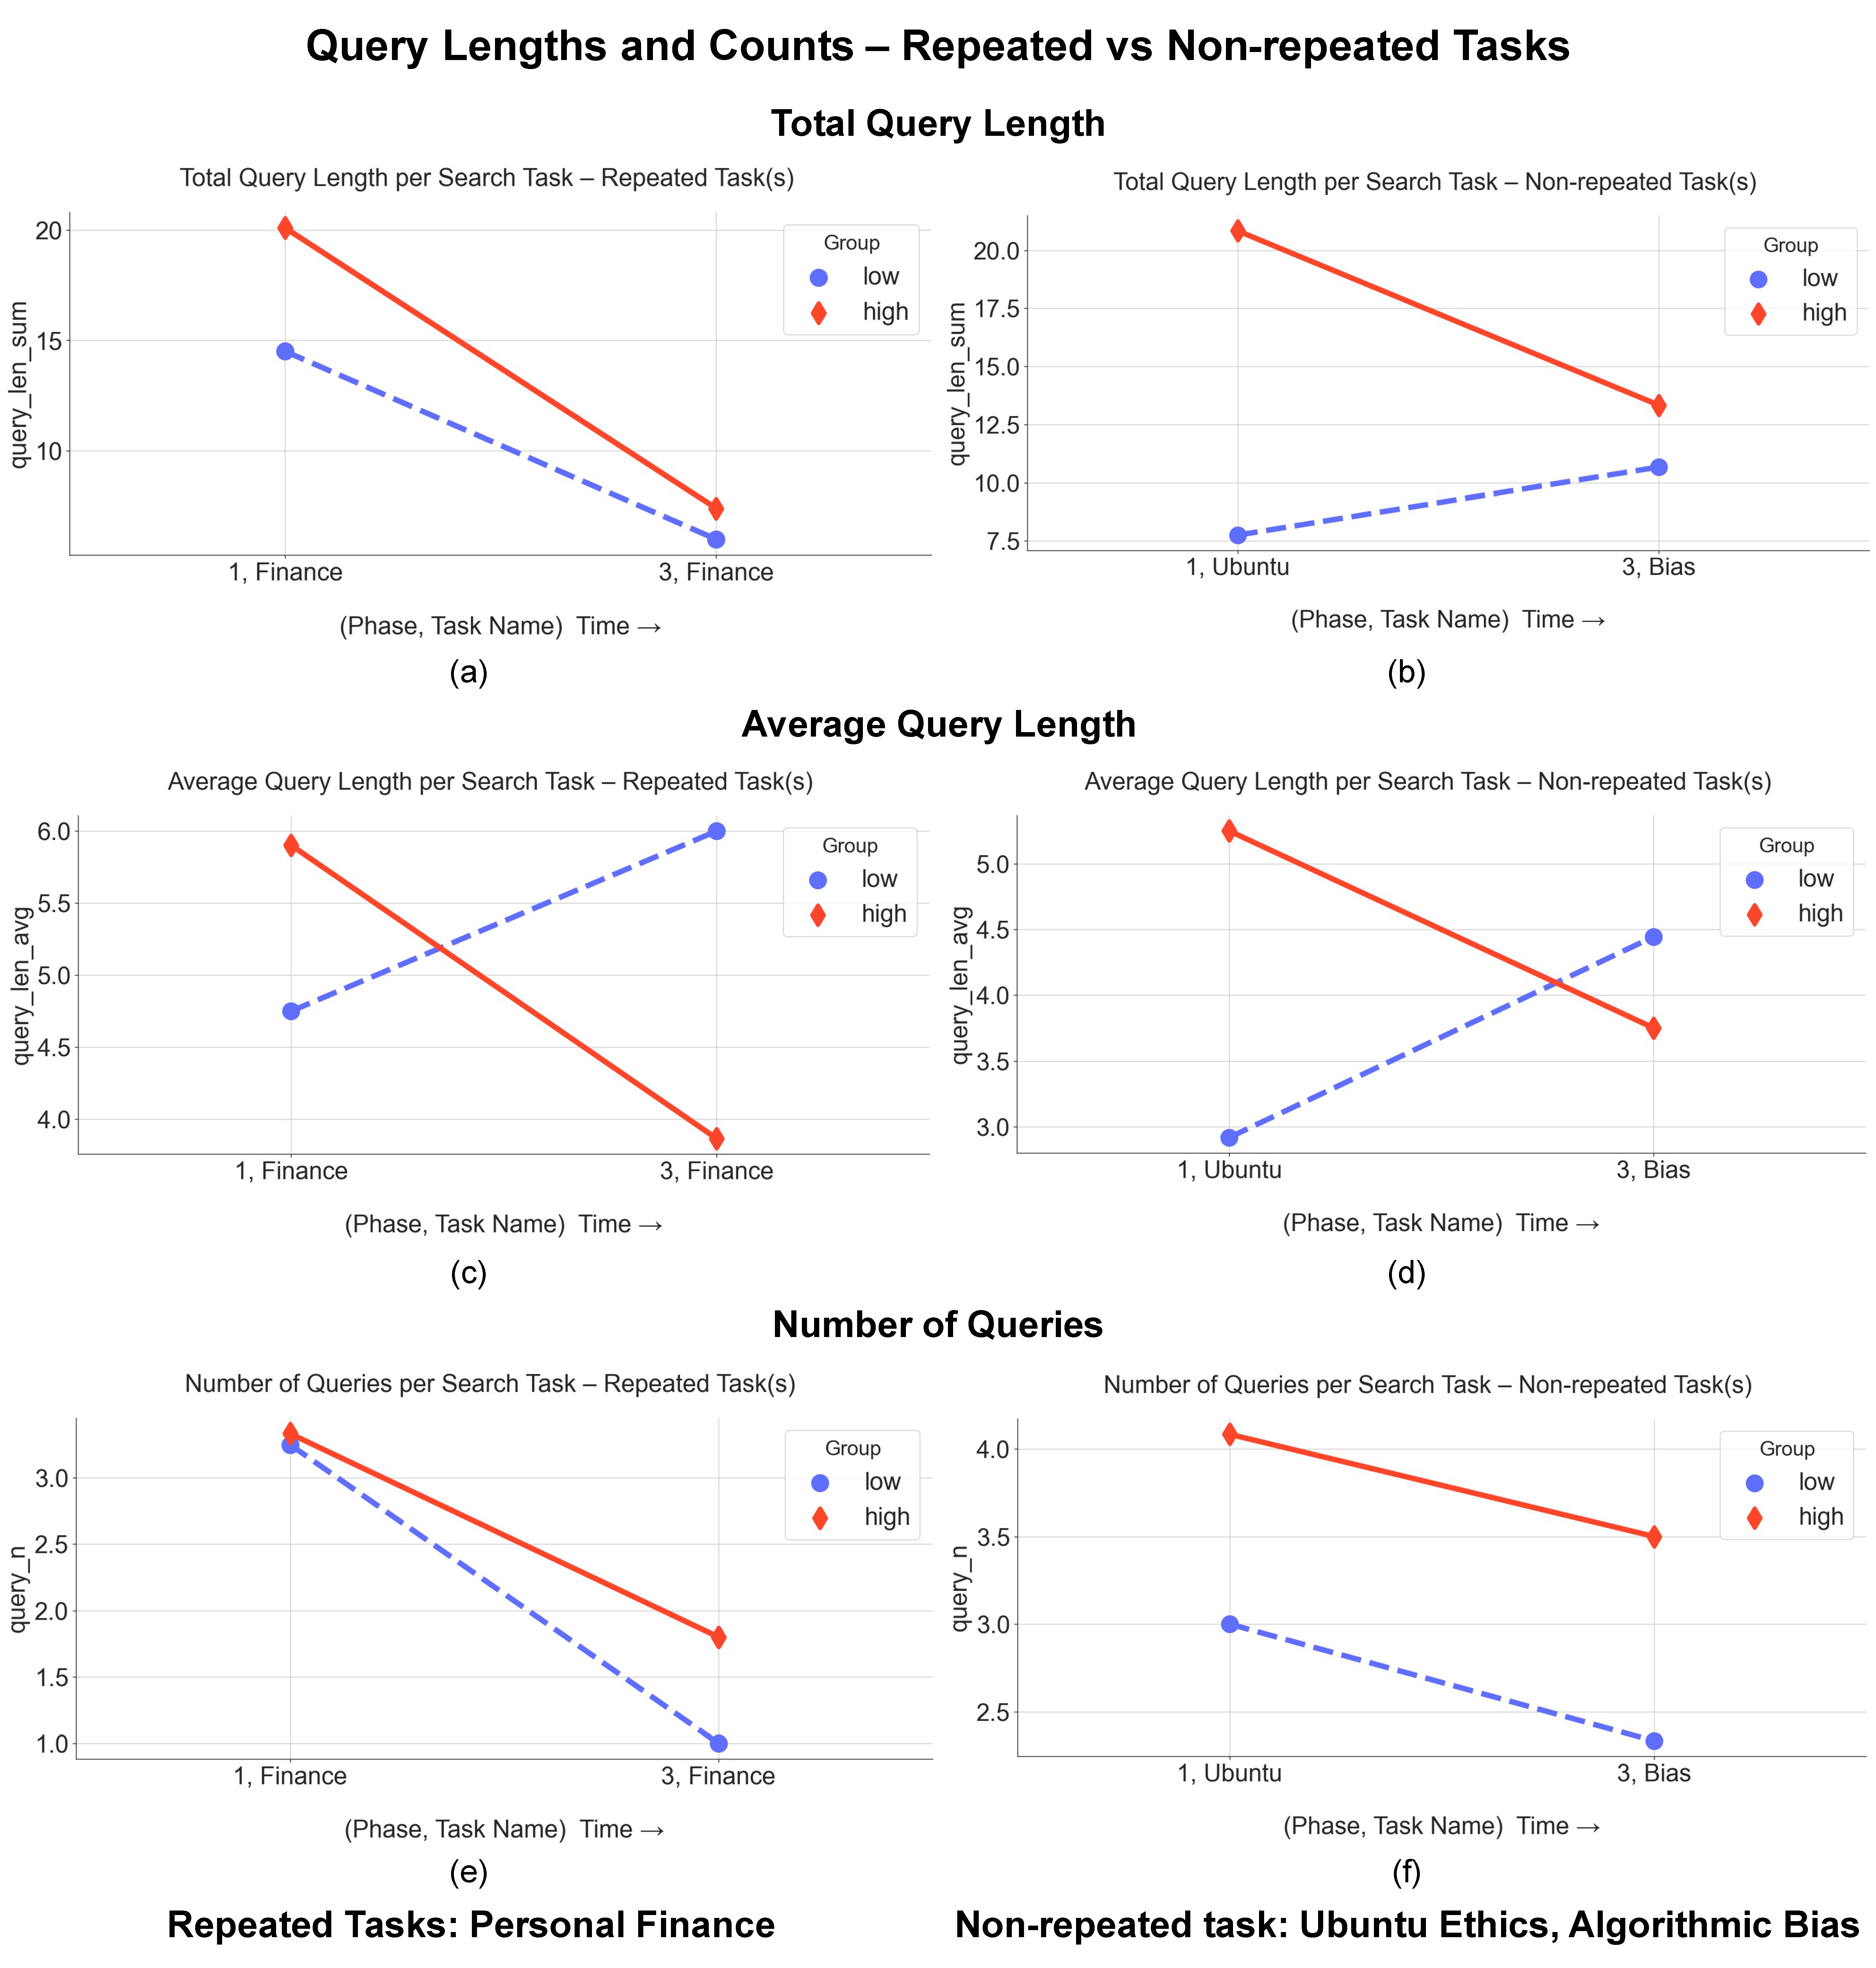
\includegraphics[width=1\linewidth]{figs/rp13-query-length-count} 

}

\caption[Query Lengths and Counts -- Repeated vs Non-repeated Tasks.]{Query Lengths and Counts -- Repeated vs Non-repeated Tasks.}\label{fig:rp13-query-length-count}
\end{figure}





Figure \ref{fig:rp13-query-length-count} shows the differences in total query length (a, b), average query length (c, d), and count of queries (e, f) for the two sets of tasks for the low and high groups.
The high group had a decrease in query count, total query length, and average query length, for all the tasks, from the beginning of the semester to the end of the semester.
The low group had a decrease in query count as well, but their average query length increased for both the repeated and the non-repeated tasks.
For the non-repeated tasks, the Algorithmic Bias task at the end of the semester was based on course content that students learnt during the semester.
So ideally they would not have needed to search for new information if they felt confident of their own knowledge.

The fact that the Algorithmic Bias task was based on course content could have influenced the search behaviour of the participants.
As we saw in Section \ref{sec-res13-need-to-search}, it is possible that the high group felt more confident in their understanding of the topic.
This was also indicated by their higher perceived learning outcome, which led them to issue fewer queries of shorter length.
On the other hand, the low group may have felt less confident with their knowledge (and presumably, search abilities), and still felt the need to explore and search for new information, leading them to issue longer queries on average at the end of the semester, in an effort to find the information they needed.

\hypertarget{query-reformulation-types-qrts-1}{%
\subsection{Query Reformulation Types (QRTs)}\label{query-reformulation-types-qrts-1}}

\begin{figure}

{\centering 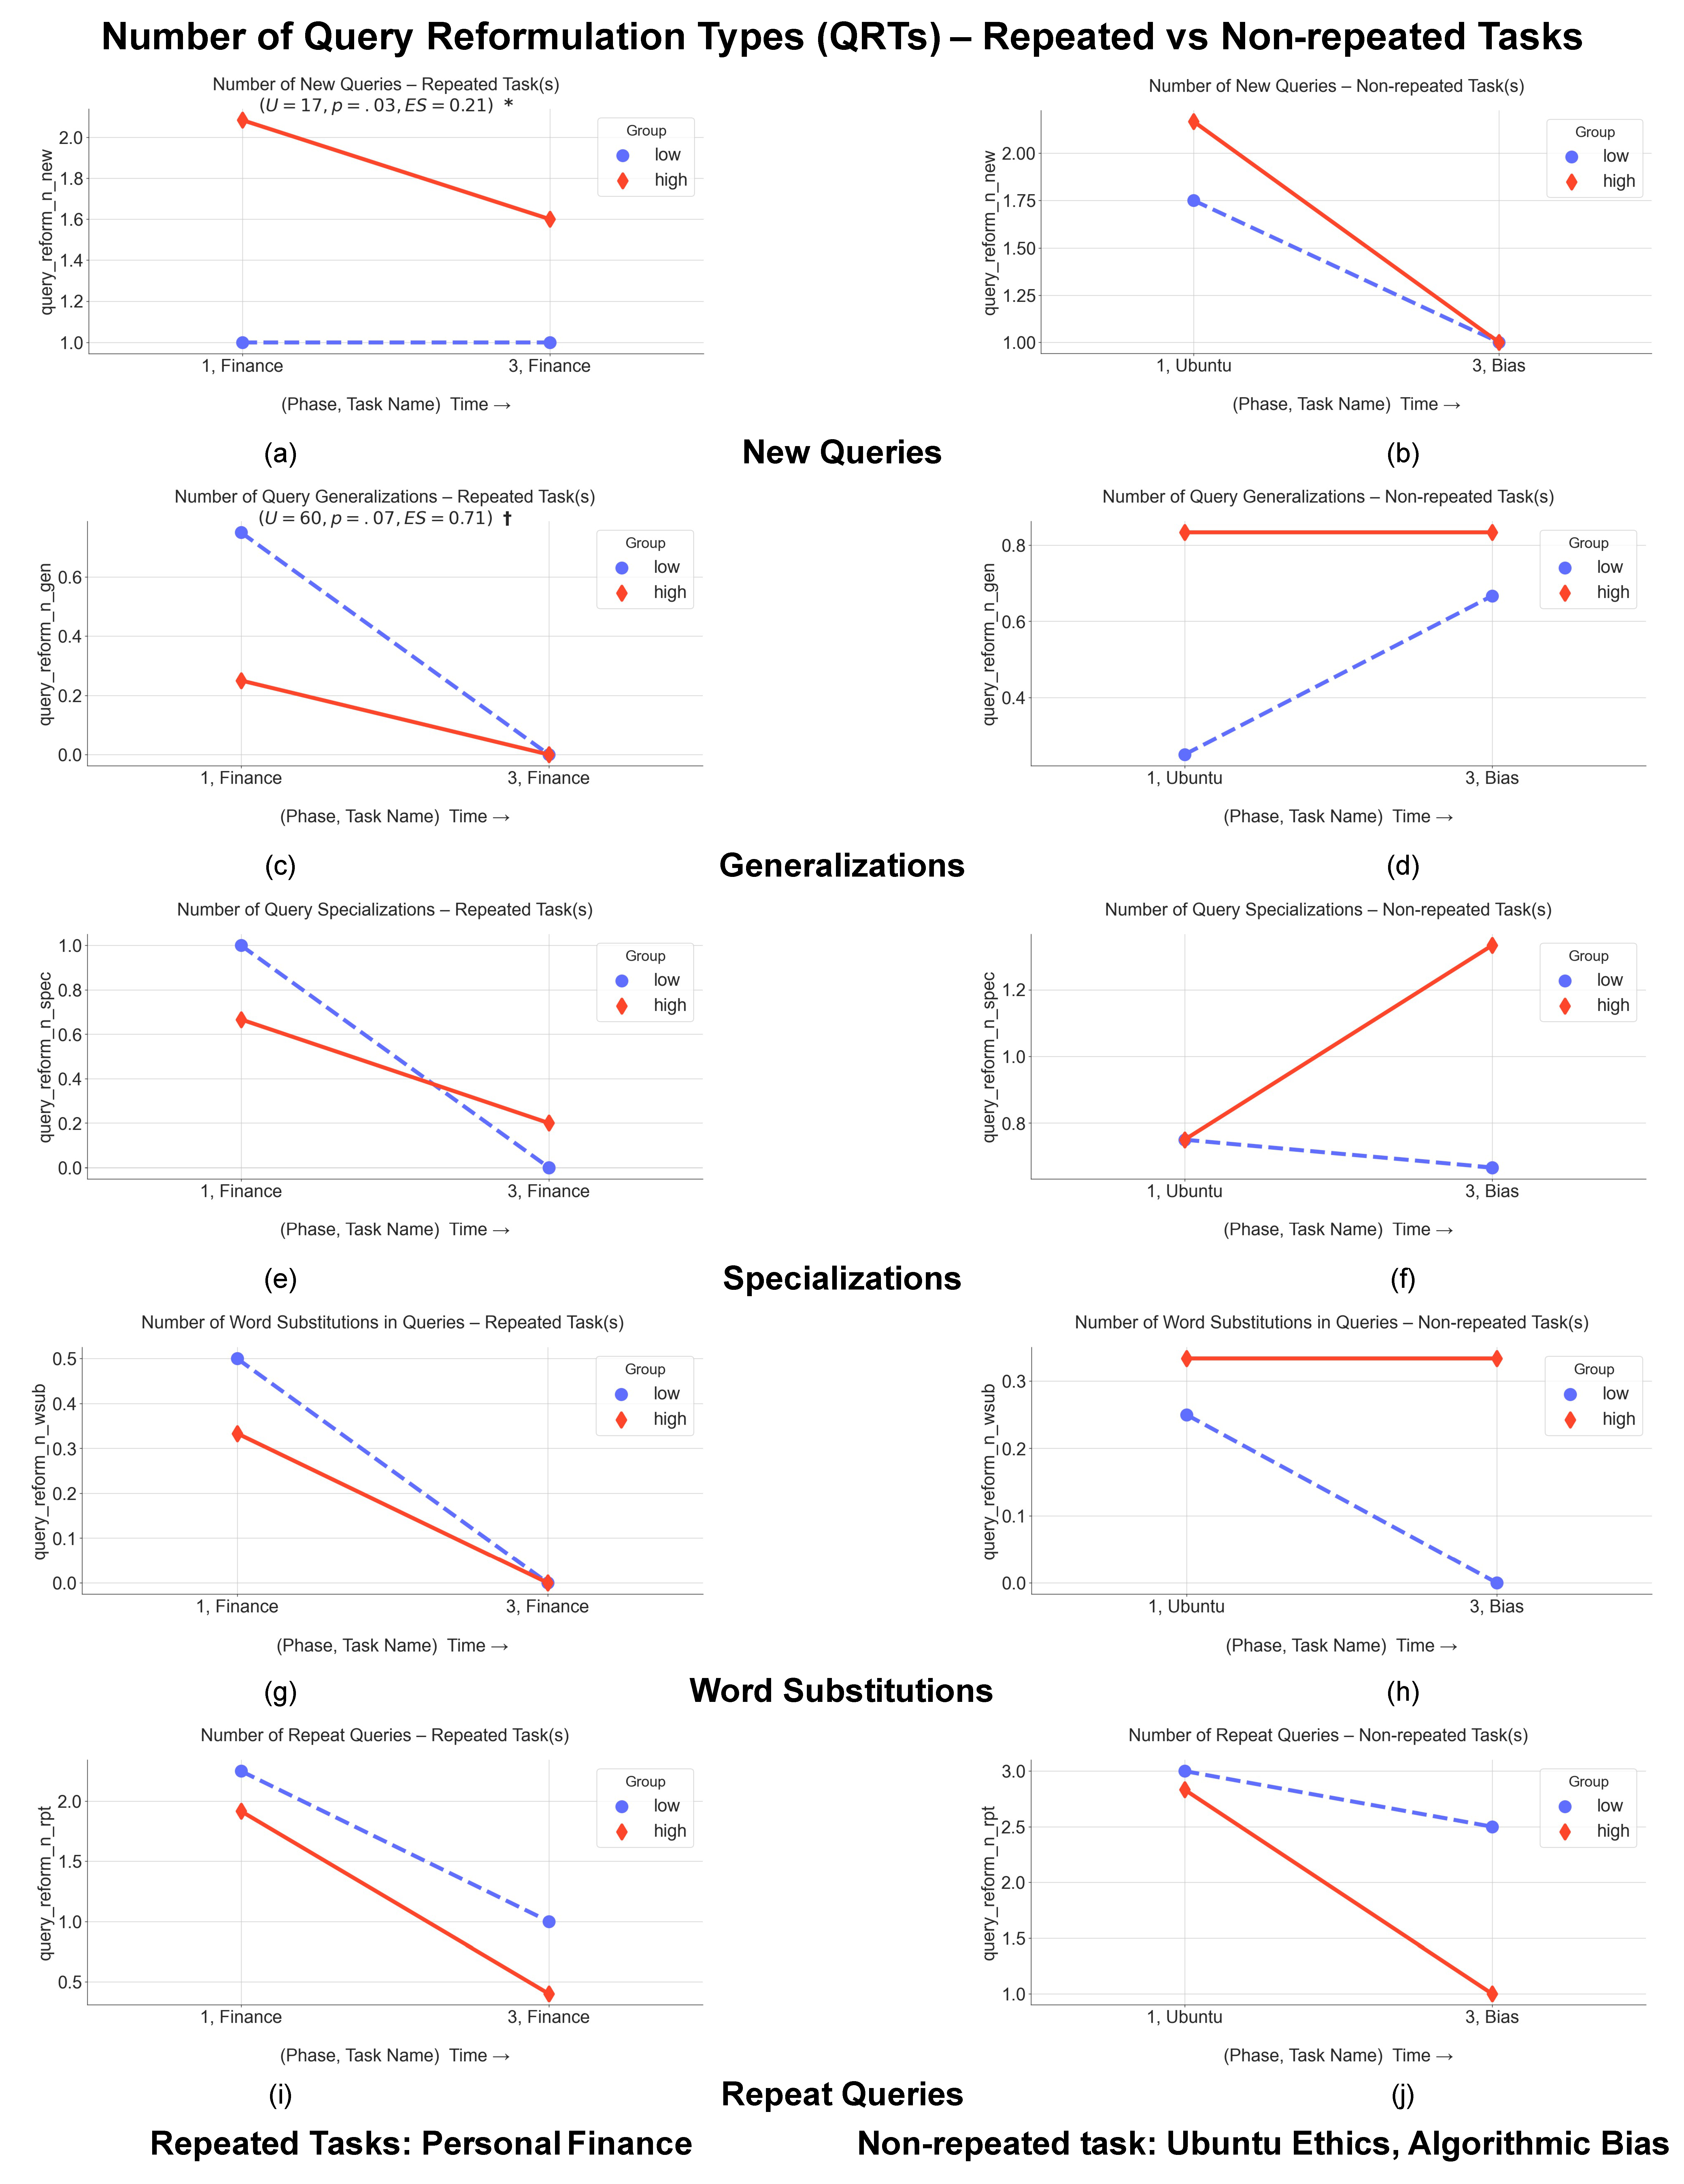
\includegraphics[width=1\linewidth]{figs/rp13-qrt} 

}

\caption[Number of Query Reformulation Types (QRTs) -- Repeated vs Non-repeated Tasks.]{Number of Query Reformulation Types (QRTs) -- Repeated vs Non-repeated Tasks.}\label{fig:rp13-qrt}
\end{figure}





Figure \ref{fig:rp13-qrt} shows the differences in the five categories of query reformulations (QRTs) for the two sets of tasks, for the low and high groups.
Both the groups showed a decrease in all query reformulation types from the start of the semester to the end of the semester, for both the task categories, except for certain specific cases.
For the non-repeated task, the high group had an increase in query specializations (Figure \ref{fig:rp13-qrt} (f)), while the low group had an increase in query generalizations (Figure \ref{fig:rp13-qrt} (d)).

These findings suggest that both groups improved their search skills over the course of the semester, as they needed to perform fewer query reformulations to find relevant information. However, the high group demonstrated a more nuanced approach to query reformulation, as evidenced by their increase in query specializations for the algorithmic bias task. This may suggest that the high group was able to better hone in on specific information needs and tailor their queries accordingly. On the other hand, the low group's increase in query generalizations for the same task may suggest a more broad and less focused approach to information seeking.

For the repeated task on personal finance, the decrease in all types of query reformulations for all groups indicates that participants had already acquired a baseline knowledge on the topic from the first round of searching earlier in the semester, and were able to more efficiently retrieve relevant information with fewer queries and reformulations.

\hypertarget{sec-res-phase13-query-H}{%
\subsection{Entropy of Query Reformulation Types}\label{sec-res-phase13-query-H}}

\begin{figure}

{\centering 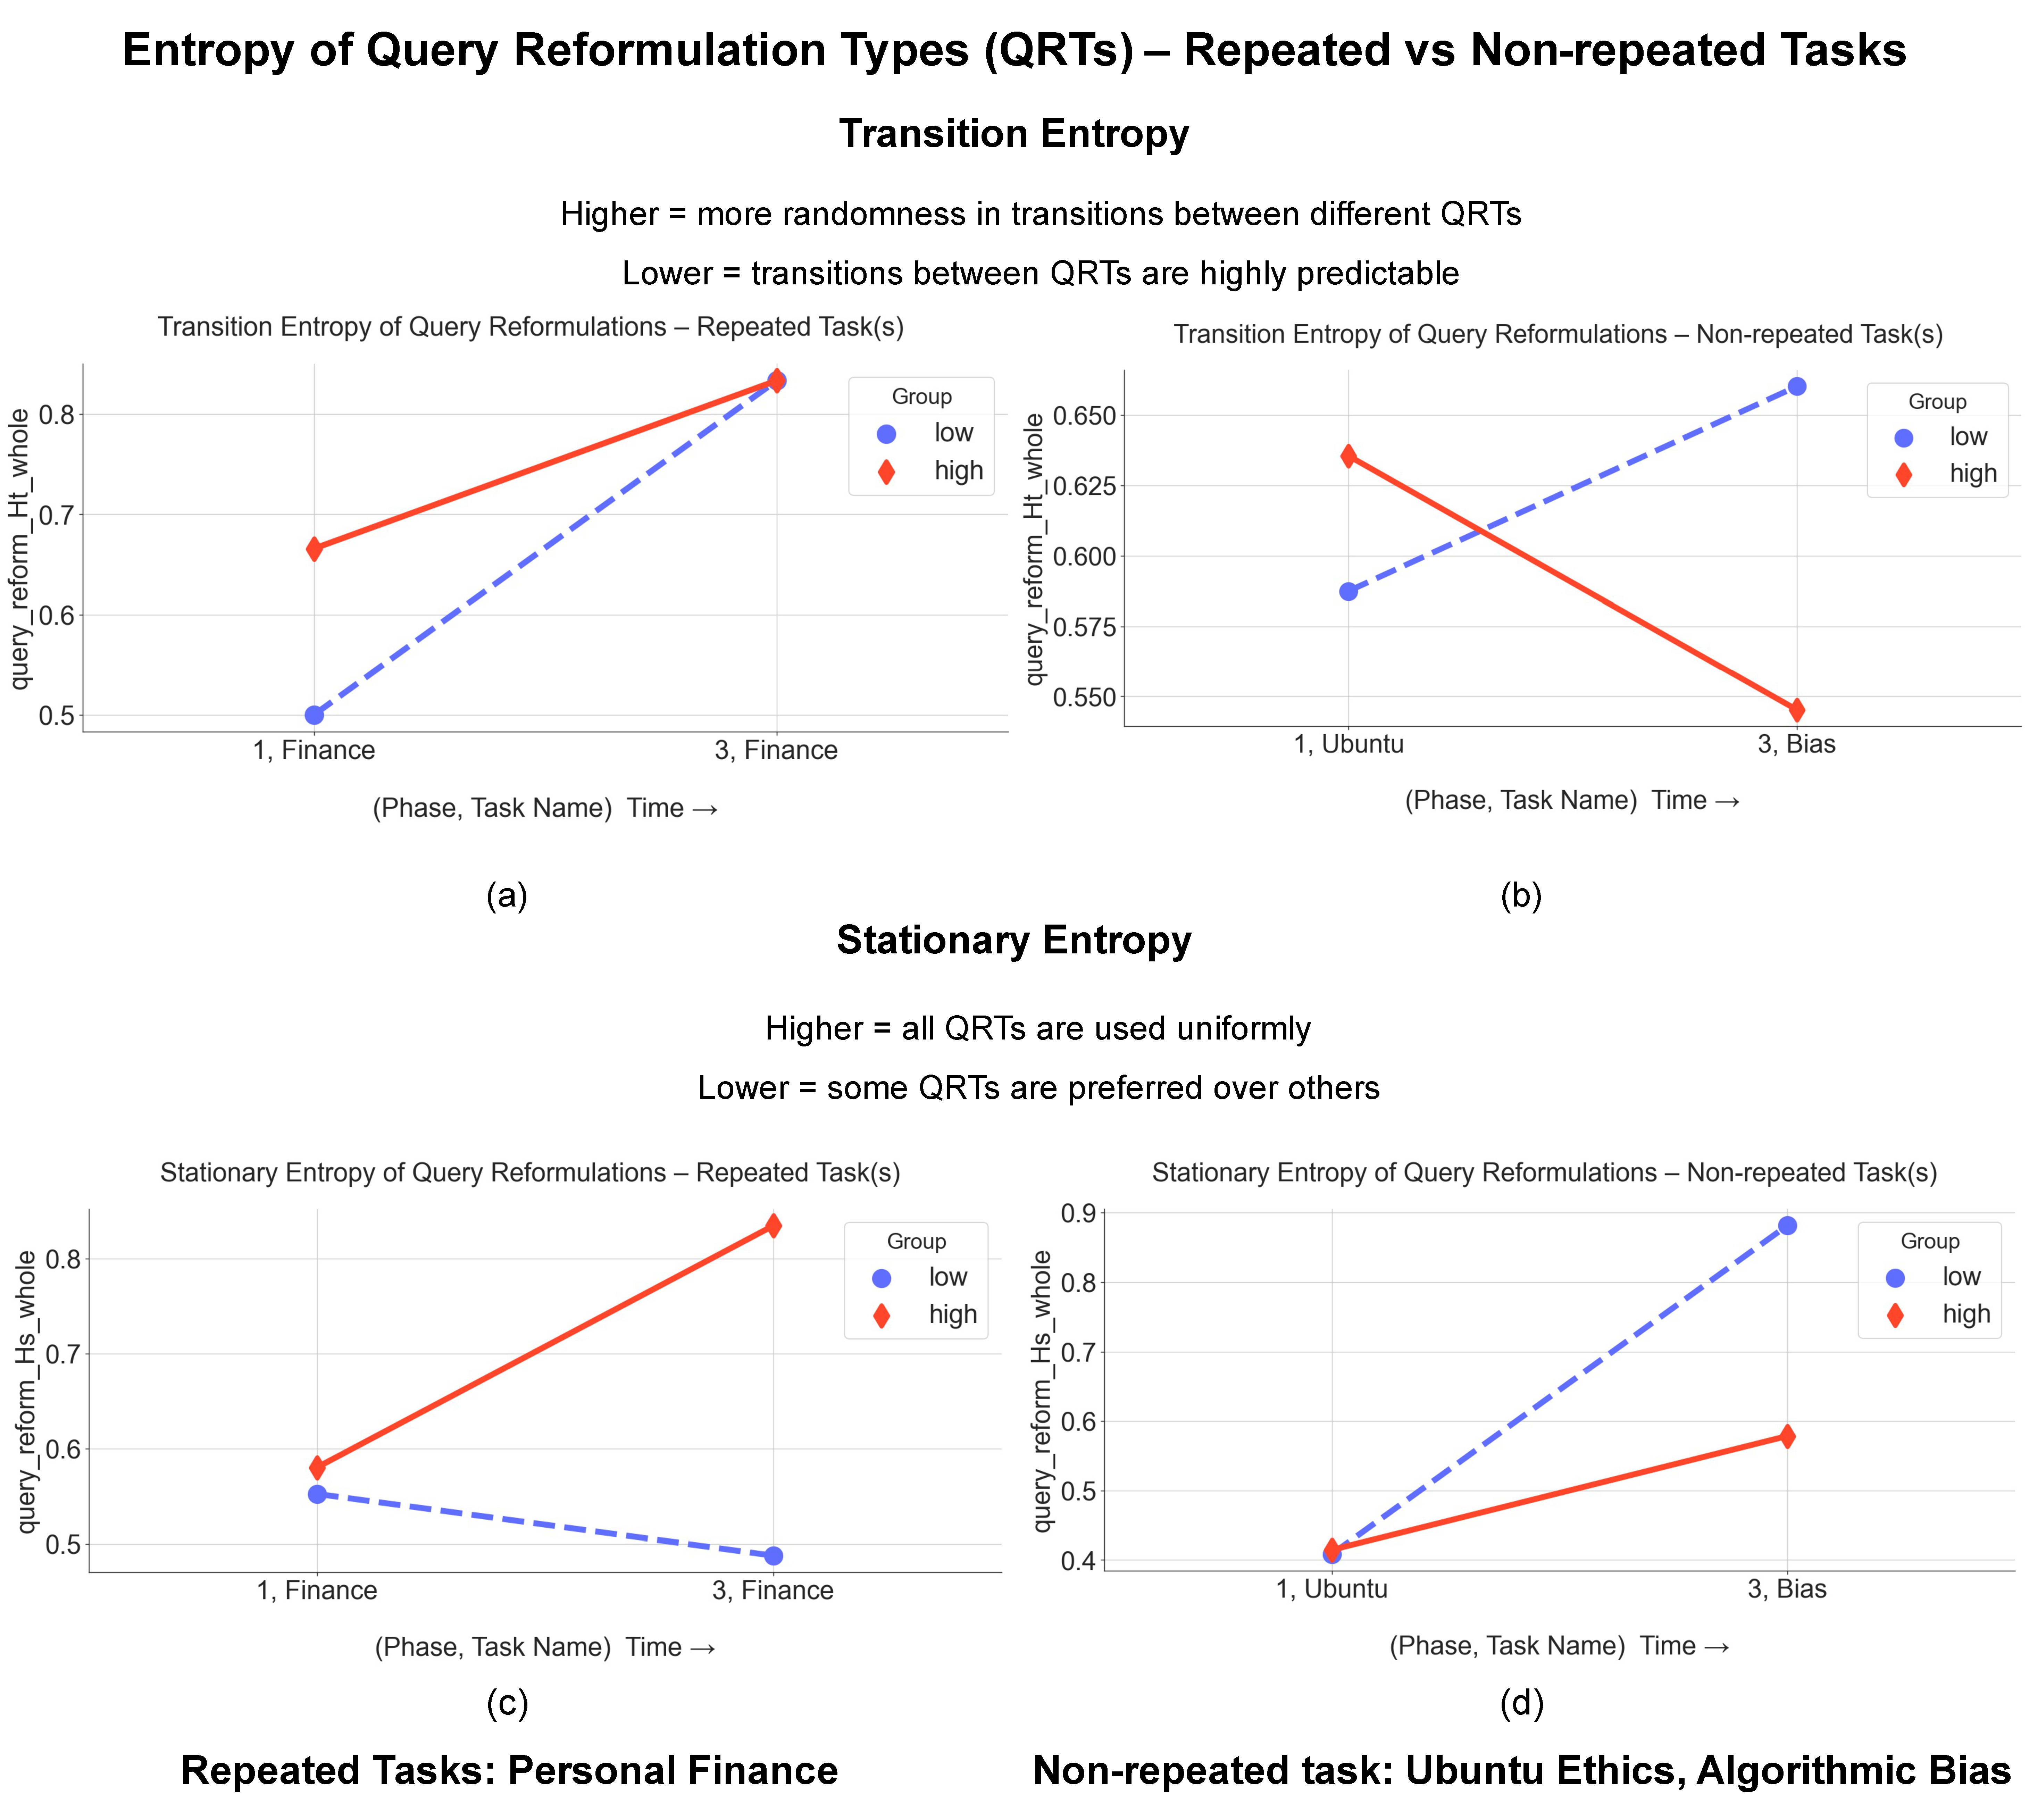
\includegraphics[width=1\linewidth]{figs/rp13-qrt-entropy} 

}

\caption[Entropy of Query Reformulation Types (QRTs) -- Repeated vs Non-repeated Tasks.]{Entropy of Query Reformulation Types (QRTs) -- Repeated vs Non-repeated Tasks.}\label{fig:rp13-qrt-entropy}
\end{figure}





Figure \ref{fig:rp13-qrt-entropy} shows the differences in the entropies of query reformulation sequences for the low and high groups, across the two sets of tasks.
For the repeated tasks on personal finance, both the groups showed an increase in transition entropy of query reformulations from the beginning of the semester to the end.
Regarding the stationary entropy of query reformulations, it increased for the high group across the semester, and decreased for the low group.
Coming to the non-repeated tasks of Ubuntu Ethics and Algorithmic bias, the high group had a decrease in transition entropy and increase in stationary entropy. The low group showed increase in both stationary and transition entropy.

The increase in transition entropy of query reformulations for both groups in the repeated task on personal finance suggests that participants were exploring different avenues and perspectives as they continued their search. This could be attributed to the fact that they were trying to find alternate information than what they had previously encountered in the beginning of the semester.
The increase in stationary entropy of query reformulations for the high group across the semester indicates that their search queries became more diverse and exploratory as they gained a deeper understanding of the topic. On the other hand, the decrease in stationary entropy for the low group suggests that they became more focused and narrowed down their search queries as they progressed through the semester.

For the non-repeated tasks, the decrease in transition entropy and increase in stationary entropy for the high group on Ubuntu Ethics and Algorithmic bias indicate that they were able to refine their search queries and find more relevant information as they gained a deeper understanding of the topics. On the other hand, the increase in both stationary and transition entropy for the low group suggests that they struggled with finding relevant information and had to explore more avenues to refine their search queries.

\hypertarget{number-of-clicks-per-query-1}{%
\section{Number of Clicks per Query}\label{number-of-clicks-per-query-1}}

\begin{figure}

{\centering 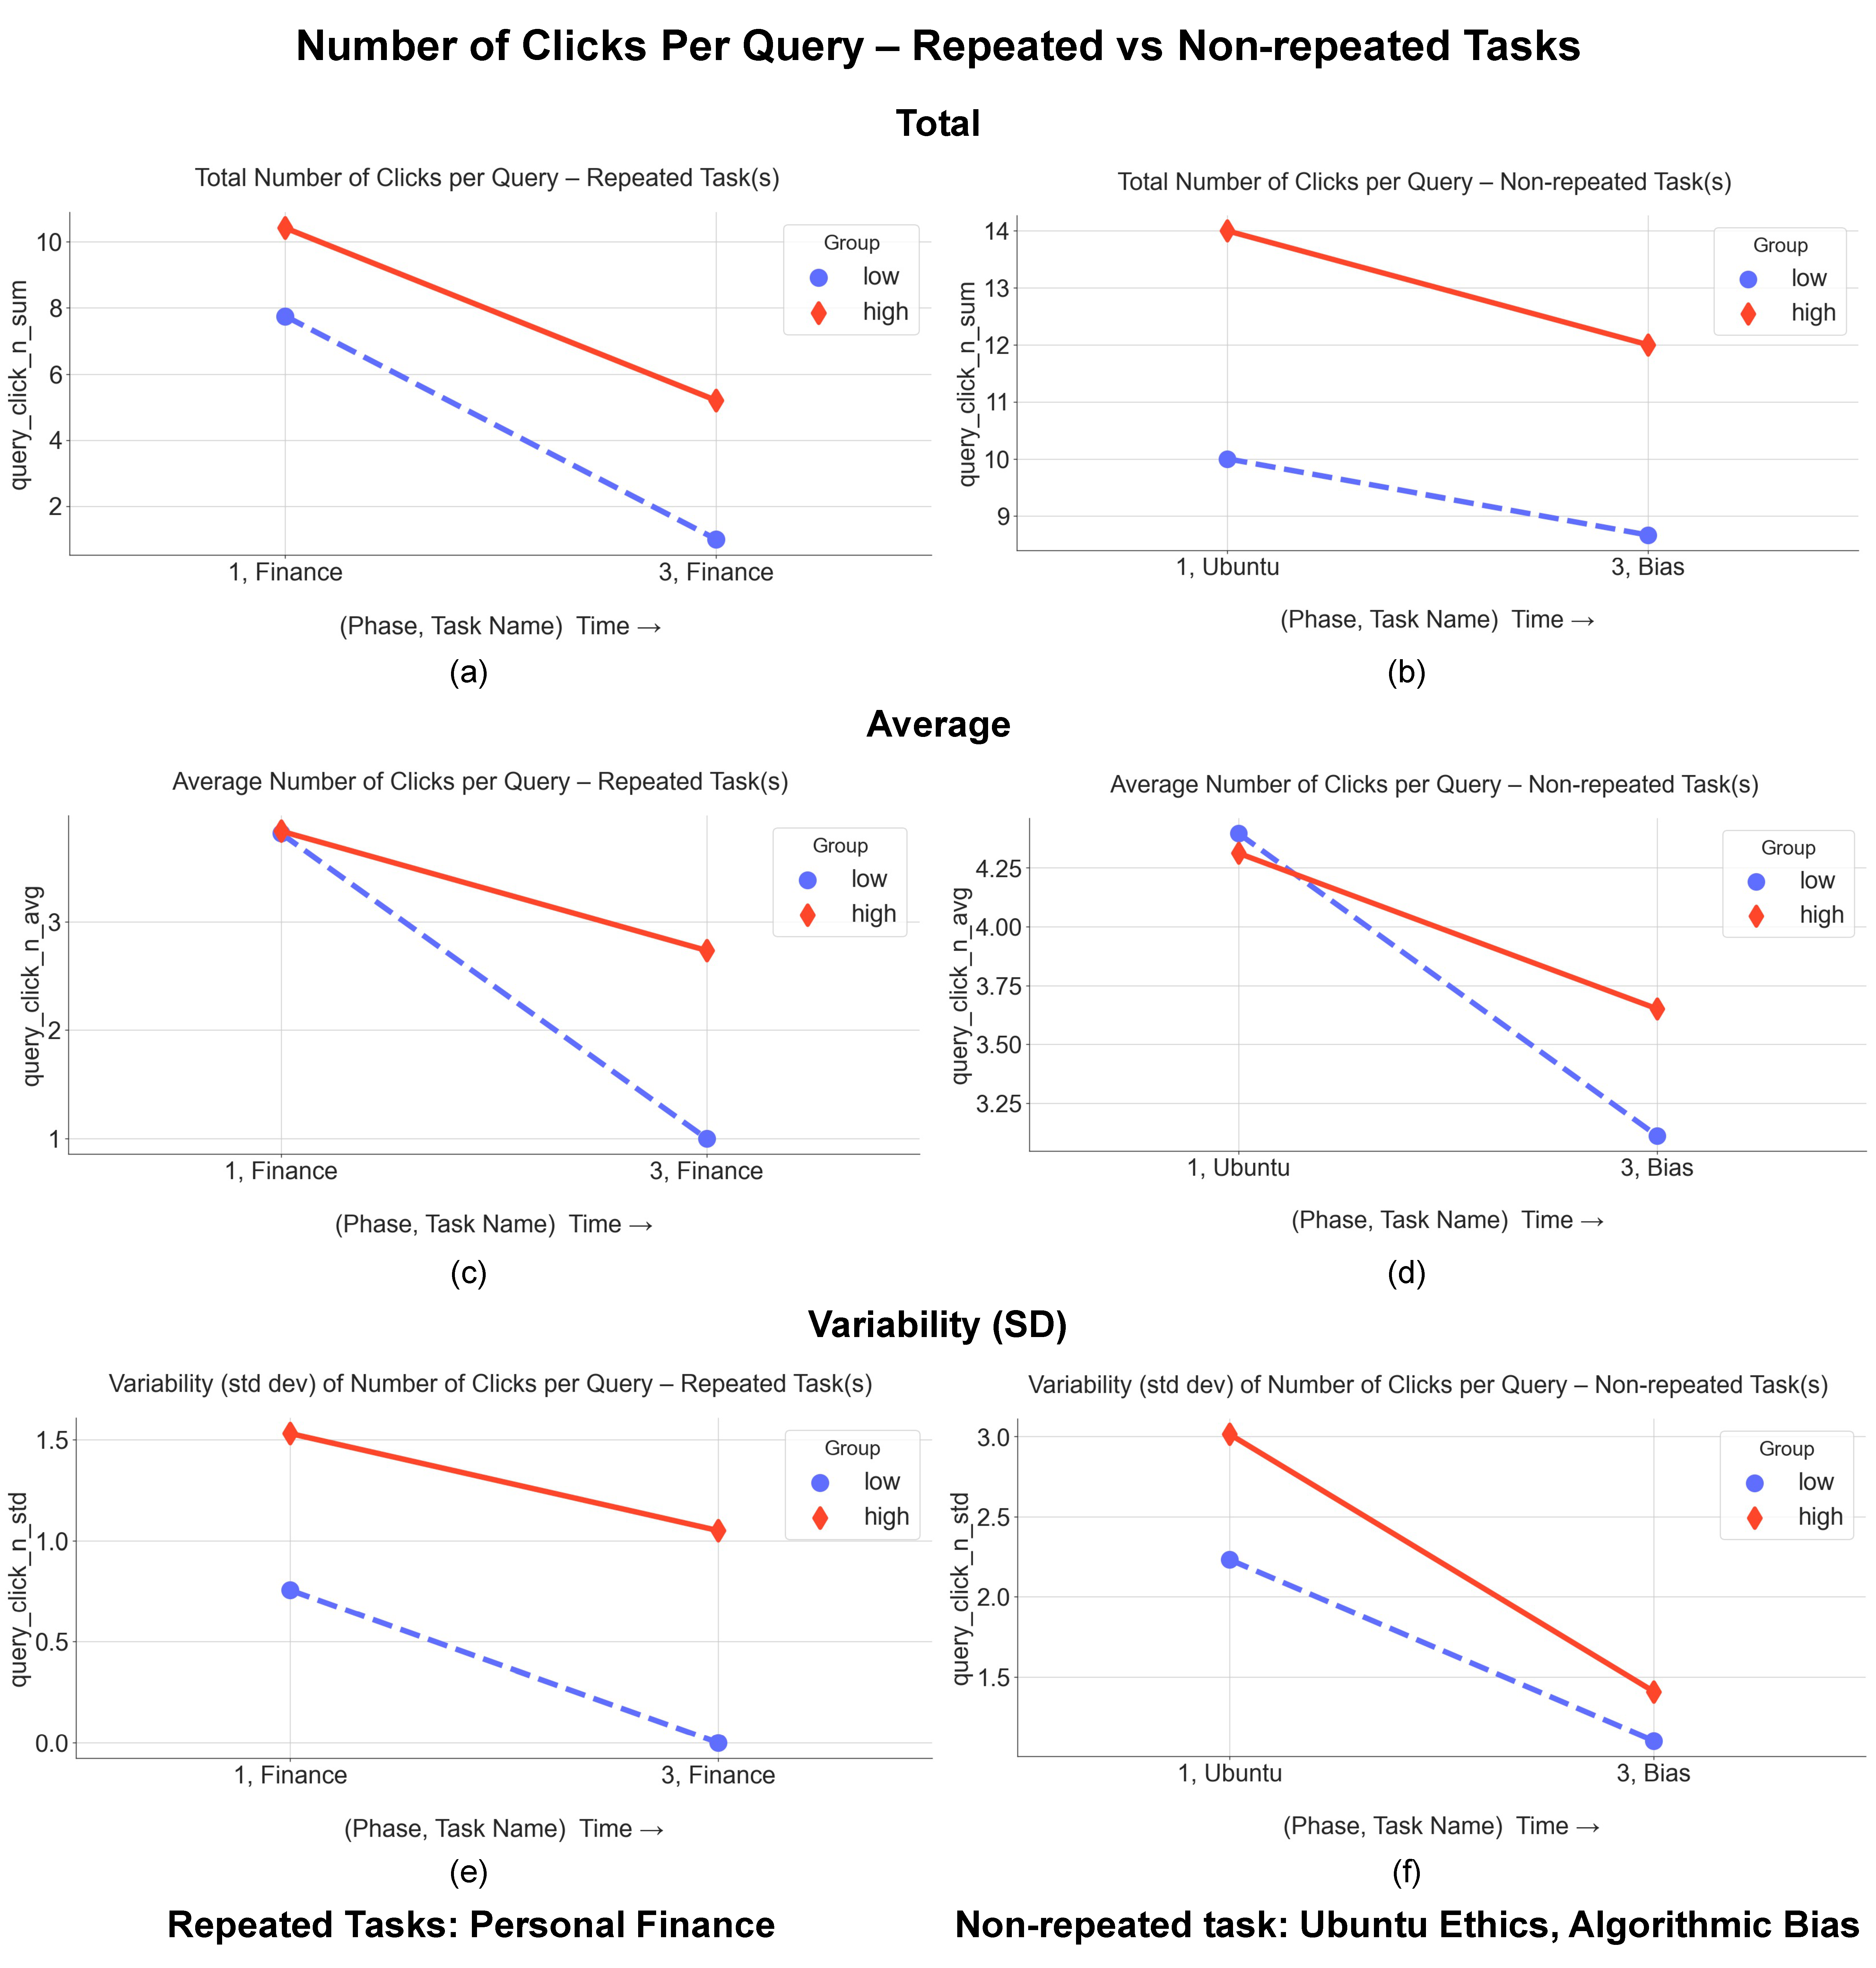
\includegraphics[width=1\linewidth]{figs/rp13-query-click} 

}

\caption[Number of Clicks Per Query -- Repeated vs Non-repeated Tasks.]{Number of Clicks Per Query -- Repeated vs Non-repeated Tasks.}\label{fig:rp13-query-click}
\end{figure}





Figure \ref{fig:rp13-query-click} shows the differences in total, average, and variability of clicks per for the low and high groups, across the two sets of tasks.
Across the board, all the groups had a decrease in the count of clicks per query for all the tasks, from the beginning to the end of the semester.

The decrease in clicks per query for both groups over time could be due to an increase in search experience and familiarity with the topics, as well as improved search strategies and tactics developed over the course of the semester.
As participants became more familiar with the topics, they likely needed to click on fewer search results to find the information they were looking for. This is because they may have developed a better understanding of what search terms to use, what types of sources to look for, and how to evaluate the relevance and reliability of search results.
This increased familiarity and experience likely contributed to the decrease in clicks per query observed in both groups over time.
Additionally, as participants developed more effective search strategies and tactics over the course of the semester, they may have been able to find the information they needed more quickly, resulting in a decrease in the count of clicks per query.

\hypertarget{l-vs-i-interaction-with-search-results-vs-content-pages}{%
\section{L vs I: Interaction with Search Results vs Content Pages}\label{l-vs-i-interaction-with-search-results-vs-content-pages}}

\begin{figure}

{\centering 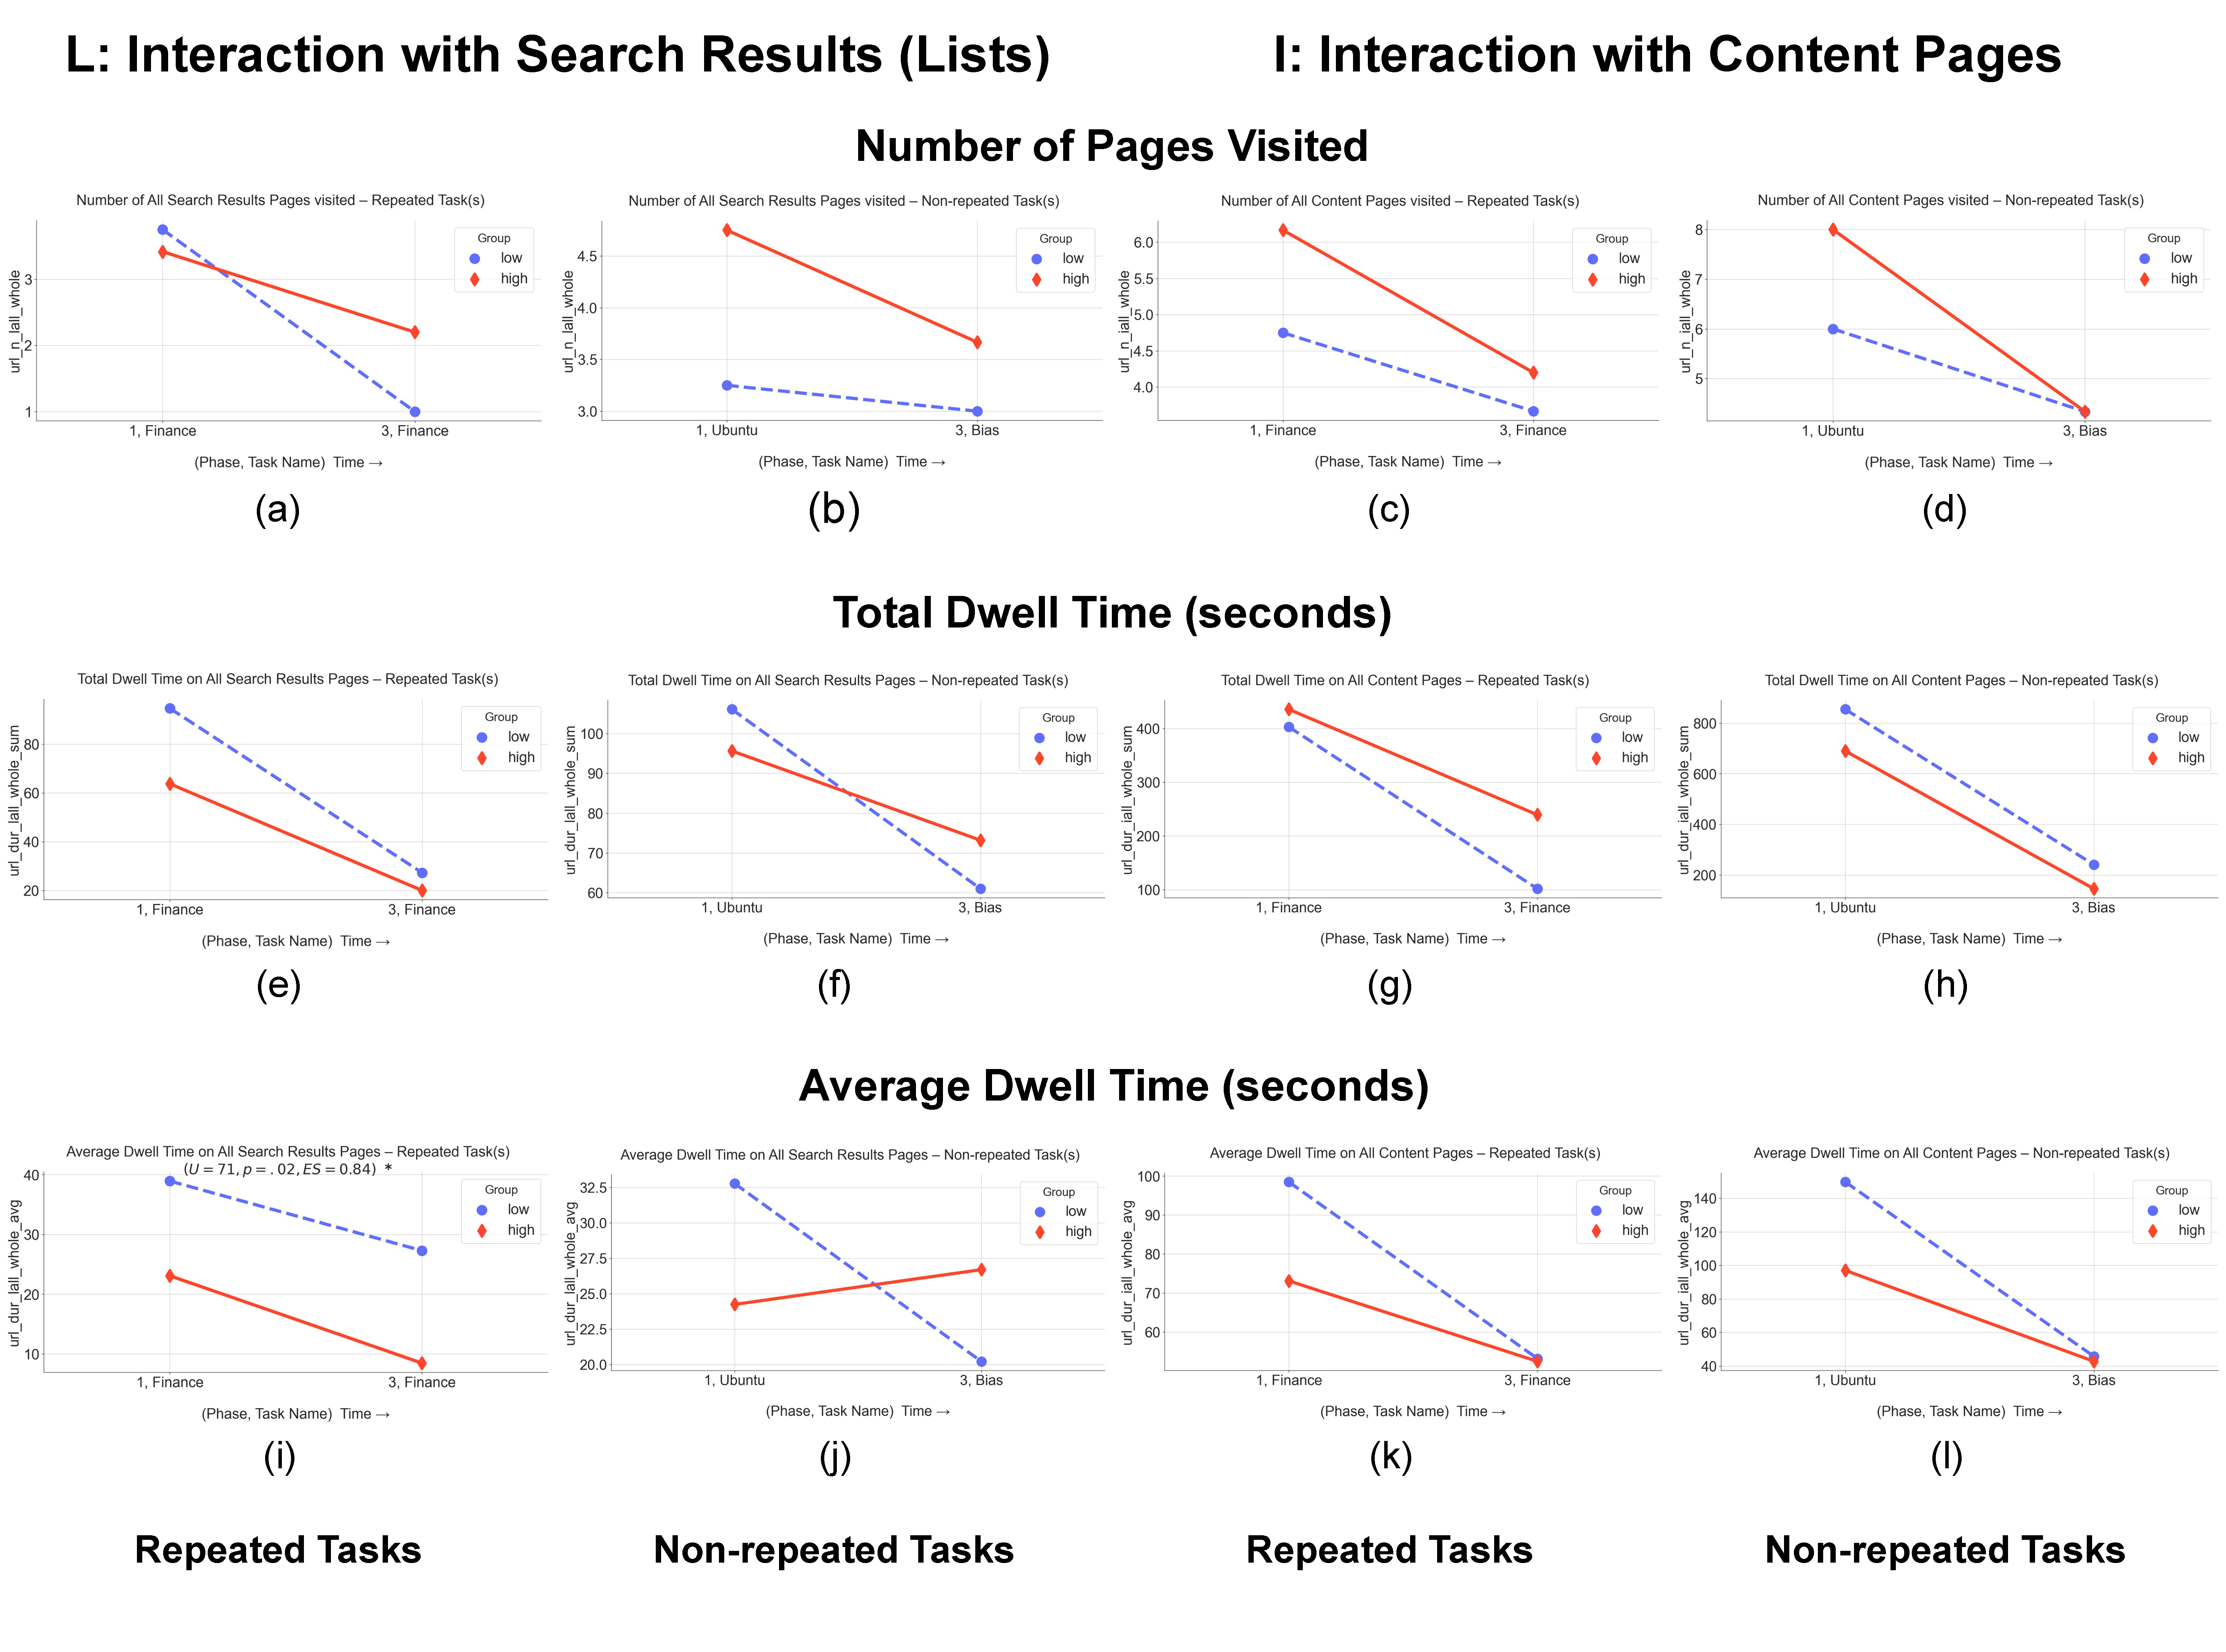
\includegraphics[width=1\linewidth]{figs/rp13-lvi} 

}

\caption[Differences in interactions with search results vs.~content pages - repeated and non-repeated tasks.]{Differences in interactions with search results vs.~content pages - repeated and non-repeated tasks.}\label{fig:rp13-lvi}
\end{figure}





Figure \ref{fig:rp13-lvi} shows the differences in interactions with search results and interaction with content pages for the low and high groups, across the two sets of tasks.
Similar to the number of clicks per query, there was an overall decrease from semester beginning to semester end, for number of pages visited, total dwell time, and average dwell time, across all types of webpages -- search results and content pages.
This could be due to an increase in search experience and familiarity with the topics, as well as improved search strategies and tactics developed over the course of the semester. As students become more familiar with the topics and develop better strategies for searching, they may have been able to quickly identify and access the information they needed, leading to a decrease in dwell time, and the number of pages visited.
These decreases may also be related to the fact that students may have become more efficient in their search process over time. They may have learned to quickly identify and assess the relevance of search results and content pages, leading to a more targeted approach in their search process.

\hypertarget{entropy-of-search-tactic-sequences-1}{%
\section{Entropy of Search Tactic Sequences}\label{entropy-of-search-tactic-sequences-1}}

\begin{figure}

{\centering 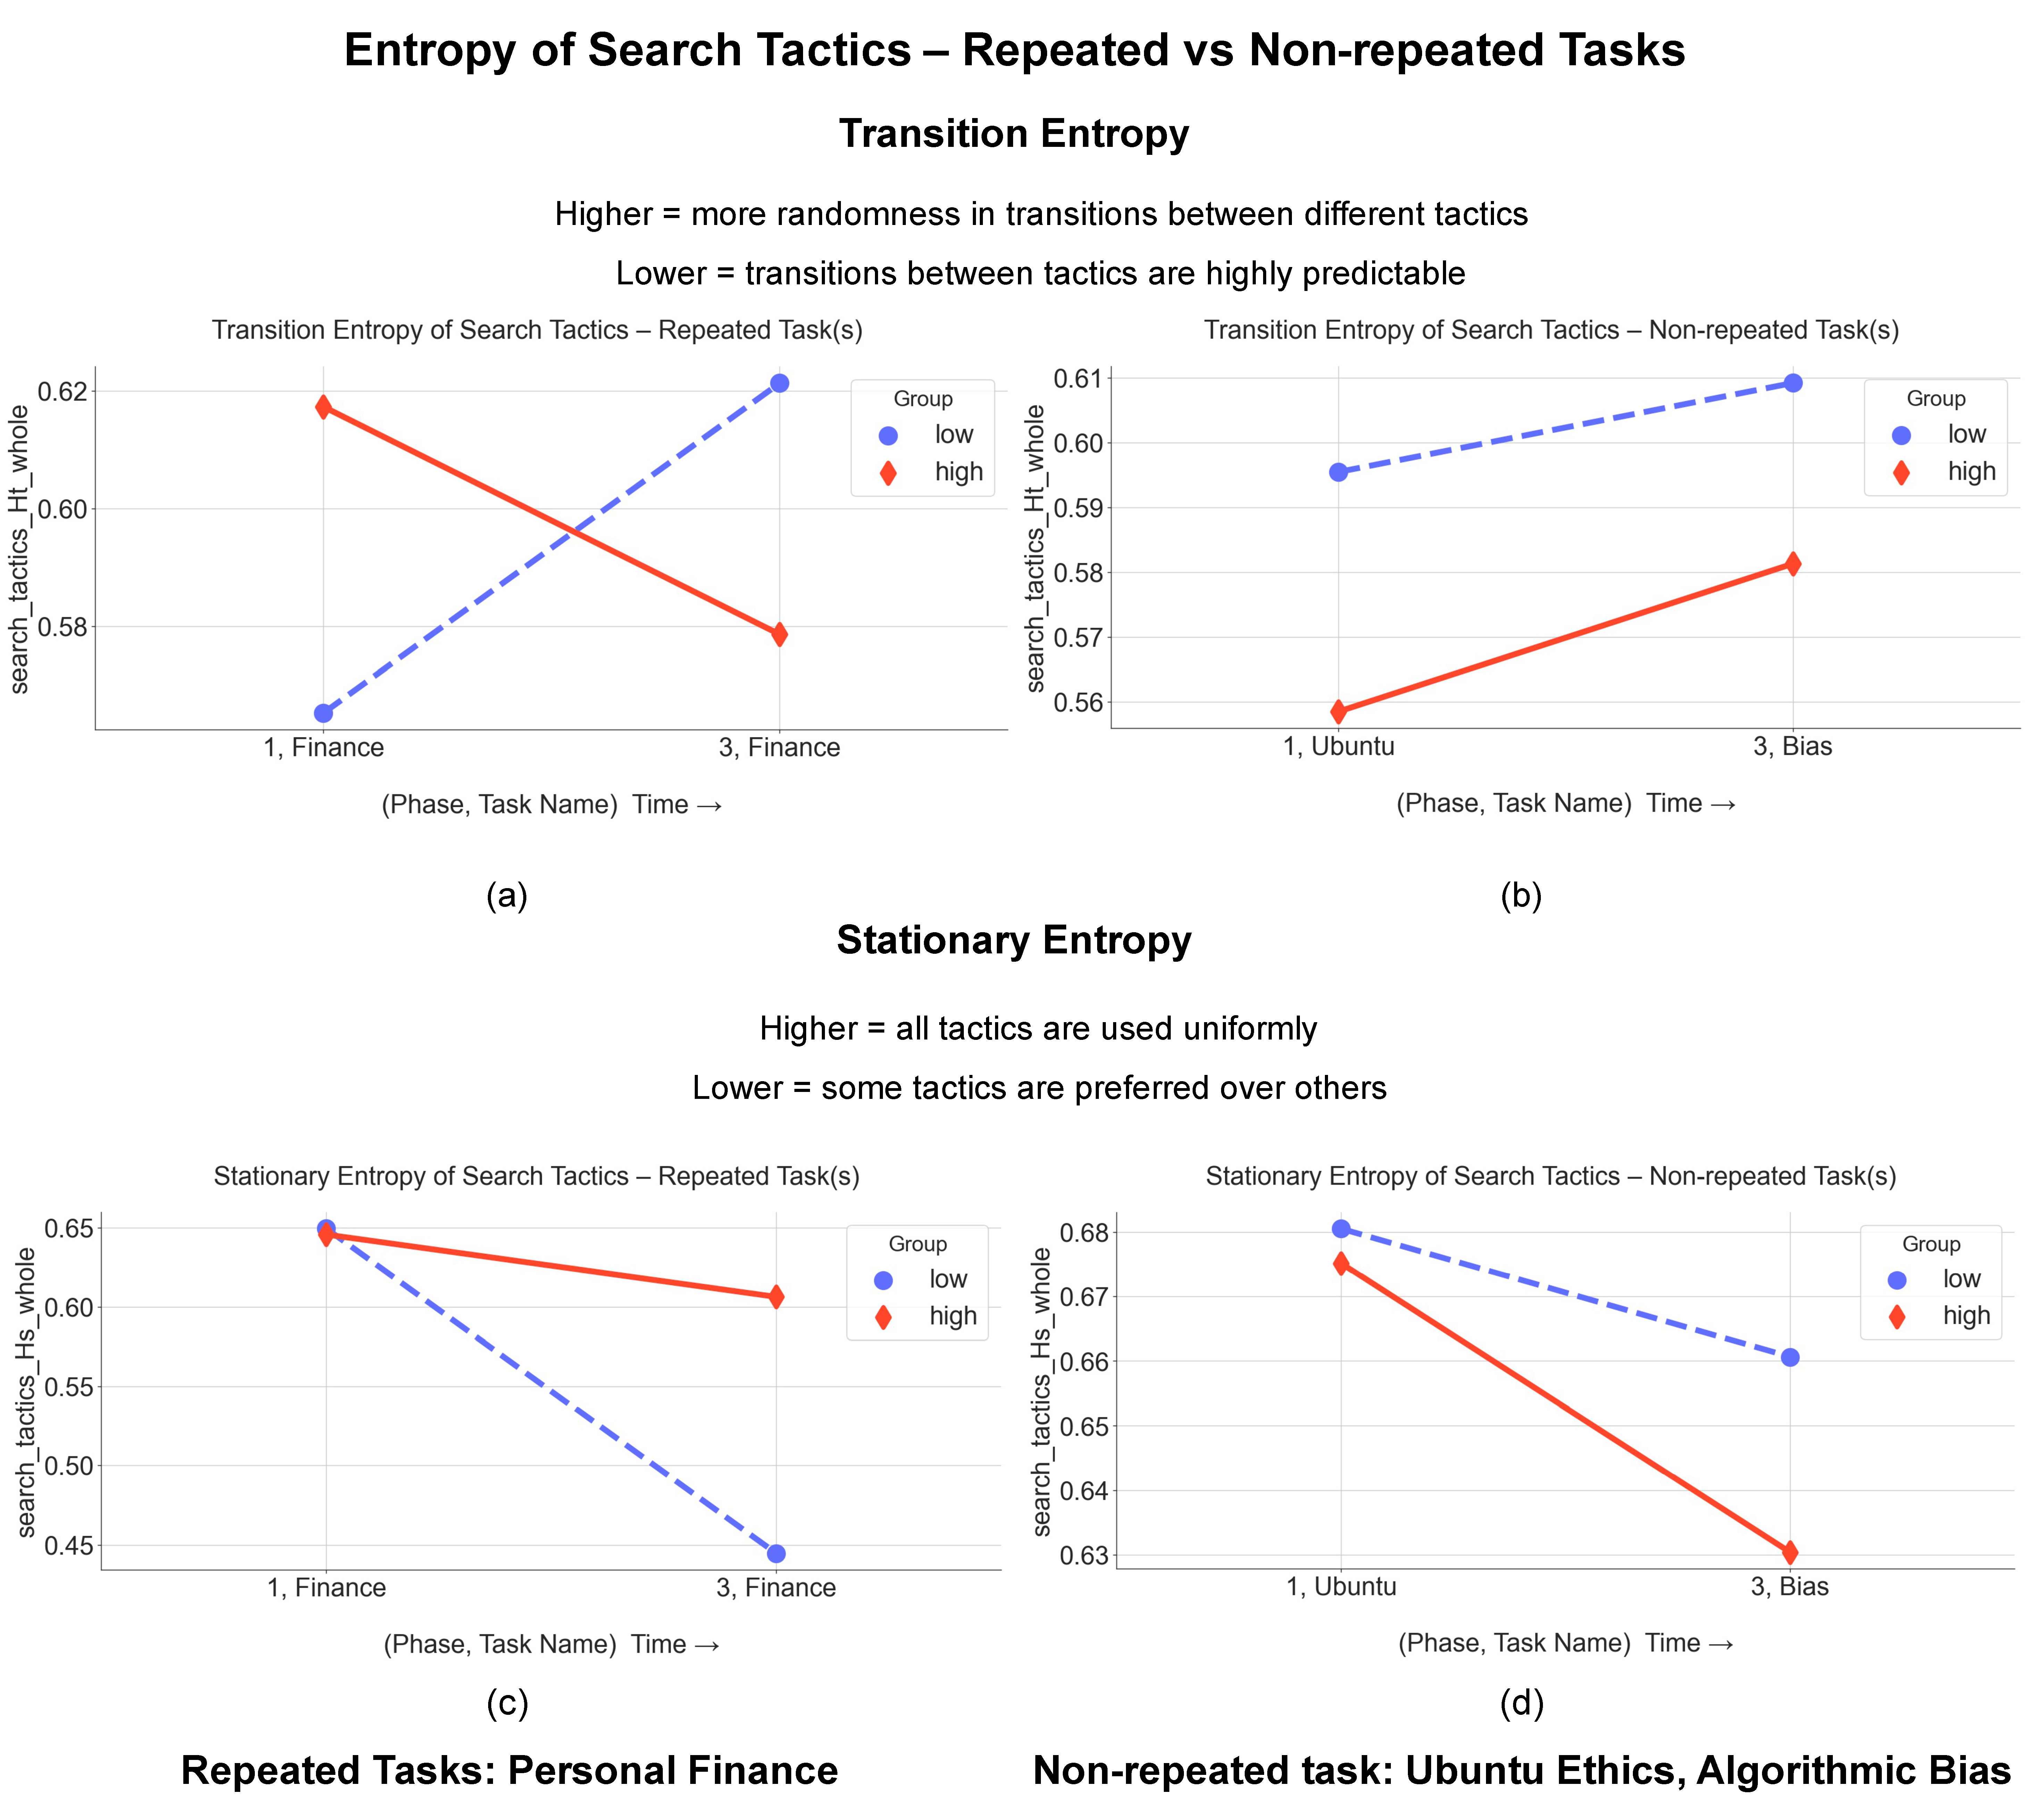
\includegraphics[width=1\linewidth]{figs/rp13-tactic-entropy} 

}

\caption[Entropy of Search Tactics -- Repeated vs Non-repeated Tasks.]{Entropy of Search Tactics -- Repeated vs Non-repeated Tasks.}\label{fig:rp13-tactic-entropy}
\end{figure}





Figure \ref{fig:rp13-tactic-entropy} shows the differences in the entropies of search tactics for the low and high groups, across the two sets of tasks.
Across the semester, the high group had a decrease in both transition entropy and stationary entropy for the repeated task, while the low group had an increase in transition entropy, but decrease in stationary entropy.
For the non-repeated task, both the groups had an increase in transition entropy, and decrease in stationary entropy.

The decrease in transition entropy and stationary entropy for the high group on the repeated tasks indicate that they were able to develop more focused and efficient search strategies over time, leading to more predictable patterns in their search tactic sequences. On the other hand, the increase in transition entropy for the low group on the repeated task suggests that they may have struggled to find effective search strategies, resulting in more varied and unpredictable sequences of search tactics. However, the decrease in stationary entropy for the low group suggests that they were still able to find and stick to effective search tactics over time.
For the non-repeated tasks, the increase in transition entropy for both groups may indicate that they were exploring a wider range of search tactics and approaches to find relevant information. The decrease in stationary entropy suggests that they were still able to identify and use effective search tactics, but that they were more flexible in their approach overall.

Comparing between the entropies for query reformulation sequences (Figure \ref{fig:rp13-qrt-entropy}) and entropies of search tactic sequences (Figure \ref{fig:rp13-tactic-entropy}), it is interesting to note that the trends of change in these two classes of entropy values were opposite for the high group, but was similar for the low group.
The high group had an increase in the transition entropy of query reformulations, but decrease in the transition entropy of search sequences, and so on.
The high group showed an increase in transition entropy of query reformulations -- meaning that they were exploring a wider range of query reformulation types over time -- but they showed a decrease in transition entropy of search tactic sequences -- indicating that they were relying on a smaller set of search tactics as they became more familiar with the topics.
Conversely, the low group showed similar trends for both types of entropies. They had an increase in both transition entropy of query reformulations and transition entropy of search tactic sequences. This suggests that the low group was still exploring different types of search strategies and query reformulation types over time, perhaps due to a lack of confidence in their own knowledge or search skills.

\hypertarget{summary}{%
\section{Summary}\label{summary}}

We summarize the findings from this chapter, on repeated vs.~non-repeated search tasks across the semester as follows.

Both the low and high groups demonstrated a general decrease in query behaviour from the start to the end of the semester
(The high group showed an increase in query specializations for the non-repeated task, and the low group showing an increase in query generalizations for the same task).
Search tactics became more random for the high group on the repeated task, and less random on the non-repeated task.
For the low group, their tactics became more random regardless of the task type.

Regarding learning and search outcomes, the high group reported higher learning and search outcomes for both repeated and non-repeated tasks at both the beginning and end of the semester.
For the low group, their perceived learning and search outcomes decreased for all tasks at the end of the semester.
The qualitative responses from participants for needing to search again at the end of the semester indicated that the high group had a stronger sense of confidence and perceived understanding of the subject-matter, compared to the low group.

The findings from the initial and final phase of the study suggest that there are differences in information search behaviours for repeated and non-repeated search tasks.
Overall, the high group demonstrated more effective and efficient search behaviour, with better search outcomes and lower entropy values, while the low group struggled with search behaviour and outcomes, showing increases in entropy values and decreased confidence in their knowledge.
This indicates that repeated engagements with search task topics may have improved the information search behaviours for the group with higher values of motivation, metacognition, self-regulation, and memory span.

\hypertarget{revisiting-research-questions}{%
\chapter{Revisiting Research Questions}\label{revisiting-research-questions}}

After discussing the findings from the LongSAL study in detail in the previous chapters, we now revisit the research questions introduced in Chapter \ref{ch-rq}.
The chapter presents a discussion of the implications of the findings of the study, in light of the research questions proposed.

\hypertarget{rq1-individual-differences-and-longitudinal-search-behaviour}{%
\section{RQ1: Individual Differences and Longitudinal Search Behaviour}\label{rq1-individual-differences-and-longitudinal-search-behaviour}}

\begin{quote}
\emph{How do (changing) individual differences of students affect their longitudinal information search behaviour?}
\end{quote}

The study found that there were (often significant) differences in information search behaviour between student groups who rated high versus low on individual traits such as motivation, metacognition, self-regulation, and memory-span.

Metacognition and self-regulation are closely related concepts that involve thinking about and controlling one's own cognitive processes and learning strategies (\protect\hyperlink{ref-ambrose2010howa}{Ambrose et al., 2010}; \protect\hyperlink{ref-garcia2023motivational}{Garcı́a et al., 2023}).
They can help students plan, monitor and evaluate their information searching and learning goals, and increase motivation and engagement (\protect\hyperlink{ref-williamson2015selfregulated}{Williamson, 2015}).
Metacognition and self-regulation can improve students' ability to learn independently and overcome barriers to learning (\protect\hyperlink{ref-winne2022metacognition}{Winne \& Azevedo, 2022}).

In the context of search as learning, metacognition can affect information searching behaviour in several ways.
Metacognition help students develop effective search queries, compare and evaluate the information obtained, identify relevant websites and sources, and reformulate queries as needed.
Students with higher levels of metacognition monitor and regulate their own search process, such as setting goals, planning strategies, checking progress and reflecting on outcomes.
Metacognition also help students improve their search performance and learning outcomes by enhancing their self-awareness, confidence and motivation (\protect\hyperlink{ref-reisouglu2020analysis}{Reisoğlu et al., 2020}; \protect\hyperlink{ref-zhou2019metacognitive}{Zhou \& Lam, 2019}).

A. Cole \& O'Brien (\protect\hyperlink{ref-cole2023using}{2023}) found that metacognitive strategies shift students' thinking away from search as a routine task towards reflections on their learning, as well as how they might apply their learning to future tasks.
One participant in their study commented that metacognitive nudges made the participant think more about what they were doing, instead of just aimlessly searching and reading a sentence or two.
Metacognition helped to give purpose to their activities, in the form of asking questions like why they were searching for a certain piece of information, and whether they would be able to talk about what they found later in group discussion settings (\protect\hyperlink{ref-cole2023using}{A. Cole \& O'Brien, 2023}).

In our study, we found that students in the high group, with higher values of metacognition, self-regulation, and motivation, demonstrated more efficient search behaviours with time.
The high group were able to better refine their search strategies and become more efficient as the semester progressed, resulting in fewer clicks per query when writing the final paper.
They had higher counts of word substitutions and lower counts of repeat queries, which are both indicative of more focused and targeted search strategies.
The randomness of their search behaviour decreased, indicating they became more efficient and strategic in their search processes.
They engaged more with content pages than search results, and reported overall better levels of learning and search outcomes.
In contrast, the low group, with lower levels of motivation, metacognition, self-regulation, and memory-span, showed less efficient search behaviours.
They showed signs of struggling, when moving across different stages of the research paper, and more clicks per query when writing the final paper.
They had more randomness and higher entropies of search tactics, more engagement with search results than content pages at later stages of the semester (which was done in earlier stages by the high group), and a general lower level of learning and search outcome.

As the high group progressed through the semester, their search behaviour gradually changed as described by established models of information seeking behaviour, such as Vakkari's searching-as-learning model (\protect\hyperlink{ref-vakkari2016searching}{Vakkari, 2016}) and Kuhlthau's Information Seeking Model (\protect\hyperlink{ref-kuhlthau1991inside}{Kuhlthau, 1991}).
Vakkari outlines three stages in the search process:
(1) assimilation,
(2) restructuring, and
(3) tuning.
According to the model's predictions, in the initial stages, students acquire knowledge through assimilation.
Bogers \& Kaya (\protect\hyperlink{ref-bogers2021exploration}{2021}) reports that searchers in this stage perform some basic `quick-and-dirty' searching in the beginning to get to know the space of available resources.
As students progressed in their search task, they increasingly demonstrate more deliberate and strategic querying behaviour.
This implies students progressively enhanced their search efficiency across the session, which has also been reported by other studies (\protect\hyperlink{ref-bogers2021exploration}{Bogers \& Kaya, 2021}; \protect\hyperlink{ref-kaya2023understanding}{Kaya \& Bogers, 2023})
This transition from divergent to convergent behaviour is also in line with Kuhlthau's information seeking model(\protect\hyperlink{ref-kuhlthau1991inside}{Kuhlthau, 1991}).

These findings also complement prior work on identifying struggling search behaviour.
For instance, Hassan et al. (\protect\hyperlink{ref-hassan2014struggling}{2014}) investigates search behaviours of users to identify signs of struggling versus exploring.
Their findings indicated that certain predictors, such as minimal similarity between consecutive queries, increased clicks per query, as well as differences in the nature of query reformulation patterns (i.e., less query term substitution and more addition/removal with exploring), were indicative of struggling search sessions.

It is important to note that the use of scholarly publications may not necessarily guarantee better quality information or higher self-perceived learning outcomes.
The relevance and credibility of the sources used, as well as the ability to critically evaluate and synthesize the information, are important factors that can impact the effectiveness of the search and learning outcomes.

The quality of information is not solely determined by the type of source, but rather by the relevance, credibility, and reliability of the information found.
While scholarly publications may provide more specialized and in-depth information, they may not always be the most relevant or up-to-date sources for a given research topic.
In these situations, web search results may provide a broader range of sources, including news articles, blogs, and websites, that can offer alternative perspectives and insights on the research topic.
However, the quality and reliability of the information found in these sources may vary, and it is important to critically evaluate and verify the information before using it in a research paper.

In addition, sensemaking -- the ability to synthesize and integrate information from different sources, regardless of their type -- is a key skill in conducting research and writing a research paper.
This involves the ability to critically evaluate the relevance and credibility of the sources, as well as to identify and articulate the relationships between different pieces of information.

Overall, the choice of sources and the search strategies used should be based on the research question, the scope of the project, and the specific information needs of the researcher. Both scholarly publications and web search results can provide valuable information, and the key is to use them effectively and efficiently in order to achieve the desired learning outcomes.

\hypertarget{rq2-repeated-vs-non-repeated-search-tasks}{%
\section{RQ2: Repeated vs Non-repeated Search Tasks}\label{rq2-repeated-vs-non-repeated-search-tasks}}

\begin{quote}
\emph{What are the similarities and differences in information search behaviours for tasks where the learning goals are new (non-repeated search tasks), versus those where the learning goals are repeated (repeated search tasks)?}
\end{quote}

Non-repeated search tasks are those where the learning goals are new and require exploration and discovery of new information.
Repeated search tasks are those where the learning goals are repeated and require reinforcement and retrieval of existing information.
The findings from this study suggest that there are similarities and differences in information search behaviours for tasks where the learning goals are new versus those where the learning goals are repeated.

Regarding \textbf{similarities}, both the high and low groups showed a decrease in query reformulation types, and count of clicks per query across the semester, regardless of whether the tasks were repeated or non-repeated.
However, there were some \textbf{differences} as well.
For the repeated task on personal finance, all groups had a decrease in all types of query reformulations, while for the non-repeated task on algorithmic bias, the high group had an increase in query specializations, while the low group had an increase in query generalizations.
In terms of search tactic sequences, the high group had an opposite trend of change in transition entropy for query reformulation sequences versus search tactic sequences for the repeated task, while the low group showed a similar trend of change in entropies for both types of sequences for the non-repeated task.

These findings complement and extend prior work that has linked topic familiarity expertise with search strategies and tactics, in influencing search behaviour.
Task familiarity and intention impacts the types of query reformulations and search tactics used (\protect\hyperlink{ref-rha2016exploring}{Rha et al., 2016}), as well as the entropy of search sequences (\protect\hyperlink{ref-he2016beyond}{He et al., 2016}).
For instance, Qu et al. (\protect\hyperlink{ref-qu2010effect}{2010}) found that task type and familiarity influenced search behaviours, such as completion time and query count, but not habitual behaviours, such as the search entrance.
Li (\protect\hyperlink{ref-li2008relationships}{2008}) reported that users' topic familiarity and task experience affected their task performance, which could lead to higher searching efficiency and effectiveness.
Finally, Karimi et al. (\protect\hyperlink{ref-karimi2011domain}{2011}) reported that topic familiarity affected query formulation strategies, such as query length, query count, use of Boolean operators and use of quotation marks.

\hypertarget{rq3-searching-behaviour-and-learning-outcomes}{%
\section{RQ3: Searching Behaviour and Learning Outcomes}\label{rq3-searching-behaviour-and-learning-outcomes}}

\begin{quote}
\emph{How do (longitudinal) information search behaviour of students relate to their (self-perceived) learning outcomes?}
\end{quote}

The study found that the participant group with higher levels of metacognition, motivation, and self-regulation demonstrated significantly higher perceived learning outcomes and search outcomes compared to the participant group which were low on these individual traits.
This also affected their longitudinal information search behaviour.

These findings are also in line with prior research, that has linked search behaviour with learning outcomes.
For instance, Weber et al. (\protect\hyperlink{ref-weber2019informationseeking}{2019}) examined a large sample of German students from all academic fields in a two-phase longitudinal study, and found that advanced levels of search behaviour and search tactics predicted better grades (\protect\hyperlink{ref-zlatkin2021students}{Zlatkin-Troitschanskaia et al., 2021}).

However, it is important to note an important limitation of the \emph{LongSAL} study: we were unable to measure the direct relationship between search behaviour and actual learning outcomes, so we relied upon self-reported perceptions of learning outcomes.
Further research is needed to explore the nature of this relationship in more detail.

\hypertarget{conclusion}{%
\chapter{Conclusion}\label{conclusion}}

\hypertarget{summary-1}{%
\section{Summary}\label{summary-1}}

\begin{quote}
\emph{``Social science exploration is a broad-ranging, purposive, systematic, prearranged undertaking designed to maximize the discovery of generalizations leading to description and understanding of an area of \ldots{} life''}

\hfill --- Stebbins (\protect\hyperlink{ref-stebbins2001exploratory}{2001})
\end{quote}

In this dissertation, an exploratory longitudinal study was conducted to investigate how students' longitudinal information search behaviours change with time, what role individual differences play in this process, and how it affects their learning and search outcomes.
The study consisted of three phases, with the main longitudinal tracking phase observing students search behaviour as they worked on a research paper final project for a class.

The findings from the study suggest that metacognition, motivation, and self-regulation are important factors that determine, direct, and sustain what students do to search and learn.
Students with high levels of these traits demonstrated higher perceived-learning and search outcomes, compared to those with low levels of these traits.
Additionally, the high group demonstrated more stable information searching behaviour over time compared to the low group.

As depicted in the opening quote from Stebbins (\protect\hyperlink{ref-stebbins2001exploratory}{2001}), our exploratory research was inductive, aiming to illuminate new concepts through observation.
We purposefully did not follow a deductive approach, which usually proves or tests an existing theory or hypothesis.
This resulted in very few statistically significant results in our findings.
However, we were more interested in discovering interesting patterns, and leave the task of confirmatory, deductive investigation to follow-up studies.

\hypertarget{contributions}{%
\section{Contributions}\label{contributions}}

Apart from the findings discussed at length in previous chapters, the LongSAL study also advances the field of Interactive IR in several aspects.

First, while the initial sample size may appear small with only 16 participants, it is important to consider the extensive amount of search log data collected from each participant over the course of the semester. This accumulation of data translates to a substantial amount of time spent on information searching by study participants, providing a robust foundation for drawing meaningful conclusions.
Considering that we collected and analysed more than 1500 minutes, equivalent to over 26 hours of search log data, it becomes evident that our study has amassed a substantial quantity of information. This large amount of data allows for a comprehensive examination of participants' information-searching behaviours, their evolution over time, and their relationship with individual differences in motivation, metacognition, and self-regulation.
By collecting such a significant volume of data, the LongSAL study possesses a strong empirical basis for reasonable and reliable findings. It provides a rich and detailed understanding of how undergraduate students engage in information searching while writing a research paper. This extensive breadth and depth of data collected bolsters the credibility and robustness of the findings, within the context of our study population.

Second, the fact that the student participants in the study were from one class is another important contribution. Previous works often examined search tasks from different classes or disciplines, which may introduce variability and make it difficult to isolate the specific effects of motivation, metacognition, and self-regulation on information-searching behaviours and learning outcomes.
By focusing on a single class and a specific research paper writing task, the LongSAL study provides a more controlled and focused approach to understanding the relationship between these factors.
This allows for a deeper exploration of how individual differences in motivation, metacognition, and self-regulation influence information-searching behaviours and learning outcomes within a consistent context.
Additionally, studying participants from one class offers the advantage of a shared learning environment and potentially similar prior knowledge and skill levels. This helps to minimize confounding variables and enhance the internal validity of our findings.
This emphasizes the unique aspect of our study and provides valuable insights into the specific dynamics of information-searching behaviours and learning outcomes within a particular educational context.

This dissertation also has some methodological contributions.
The first is to relate individual differences in motivation, metacognition, and self-regulation differences in a combined, holistic format with information search behaviour.
This was achieved through the person-centred approach of Latent Profile Analysis.
To the best of our knowledge, this is the first study in information science and IIR literature to have employed Latent Profile Analysis in such a manner.

Our second methodological contribution is the development of the YASBIL browsing logger (\protect\hyperlink{ref-bhattacharya2021yasbil}{Bhattacharya \& Gwizdka, 2021}), which was developed primarily as a response to the COVID-19 pandemic.
As human subjects research in labs came to a halt, we had to find an alternative approach to carry out IIR research.
The YASBIL logger was developed to enable us to collect data on students' online browsing behaviour as they searched for information. This tool allowed us to track students' search behaviour and analyse it in detail, providing insights into how they engage with information sources, evaluate information, and how their information search behaviour evolves over time.

Third, the URL-based classification system (Section \ref{sec-res-url-categorization}) provided a useful way to categorize webpages based on their type, allowing us to gain insights into how users' search behaviour varies across different types of webpages. By analysing the patterns of webpage types visited by users during their information search process, we were able to identify which types of webpages were most commonly visited and how they related to users' search behaviour. This information can be used to improve the design of information systems and search engines, as well as to inform the development of tailored interventions that support users' information search needs.

Together, these methodological contributions offer new ways of understanding the complex relationships between individual differences in motivation, metacognition, and self-regulation, and how they impact information search behaviour and learning outcomes. Additionally, the YASBIL browsing logger provides a powerful tool for researchers to gather detailed information about students' online browsing behaviour, making it possible to track their search behaviour and analyse it in detail. These contributions provide valuable resources for future researchers in the field of Information Science and Information Retrieval, and offer insights into how we can design more effective searching as learning environments.

\hypertarget{limitations}{%
\section{Limitations}\label{limitations}}

Like any other scientific endeavour, the LongSAL study came with its limitations.

The most prominent \textbf{theoretical limitation} of the study was the choice of learning outcomes.
Although we discuss at length about the inefficacy of traditional learning outcome measures in Chapter \ref{ch-bg-learn}, we were involuntarily forced to use two of them in this study -- self-perceived learning outcomes, and instructor assigned grades.
Our initial plan was to use Concept Maps for assessing qualitative and quantitative changes in students' learning and knowledge of concepts.
But we were limited by technology, and had to settle for self-ratings.
Education Scientists are repeatedly calling for better assessment strategies for learning (\protect\hyperlink{ref-cope2017elearningc}{Cope \& Kalantzis, 2017}; \protect\hyperlink{ref-urgo2022learning}{Urgo \& Arguello, 2022}).
Future researchers in search-as-learning must work hand in hand with educators and education researchers to investigate and apply more sophisticated forms of learning assessments, that are more equitable in the face of learner diversity.

In terms of \textbf{technical limitations}, there were a handful.
First, due to the nature of current web-technologies, we could not determine when participants were reading a PDF file on their browser.
Browser level JavaScript works only on webpages, and that is what YASBIL used to log user behaviour.
If a participant downloaded a bunch of PDFs at a given time, and read them later offline, even when turning YASBIL on, YASBIL would be blind to such readings.
Second, we could not analyze clicks on content pages. This is due to an abundance of advertisements and cookie preference popups that any user first has to encounter, before even beginning to settle on the content. This is often quite an annoyance, and also taints the dwell time measure on webpages.
Last but not the least, the low sample size is always a limitation.
We had initial hopes of recruiting about 30-40 participants for the study.
However, despite our best efforts, only 18 signed up, 16 remained till the middle of the semester, and 10 completed the entire study.
Previous literature also shows that past longitudinal studies had similar low sample sizes.
For instance, Kuhlthau (\protect\hyperlink{ref-kuhlthau2004seeking}{2004}) had 20 participants, Vakkari (\protect\hyperlink{ref-vakkari2001changes}{2001a}) had 11 and Kelly (\protect\hyperlink{ref-kelly2006measuringa}{2006a}) had 7 participants.

\hypertarget{future-work}{%
\section{Future Work}\label{future-work}}

This dissertation study was monumental effort in planning, organization, and execution.
Even after an almost 200-page dissertation, we have barely managed to scratch the surface of the amount of data that was collected in the study.

Some of the most promising directions of future work from this project include:
understanding what factors are responsible if/when students change their latent profiles at different points in the semester;
understanding parallel and cross session browsing behaviour, and how it affects learning;
deeper dive into struggling versus exploring search behaviours;
in-depth and qualitative analysis of search queries issued by participants;
understanding of long term information use;
visits and revisits to webpages, and its effects on relevance judgement;
and others.

In conclusion, this dissertation has explored the role of motivation, metacognition and self-regulation in shaping the information search behaviours and learning outcomes of students.
The findings demonstrate that differences in these individual traits are crucial components of successful searching as learning behaviour.
As Winne \& Azevedo (\protect\hyperlink{ref-winne2022metacognition}{2022}) argues, metacognition is the engine of self-regulated learning.
To help learners develop and apply productive self-regulated learning, search as learning environments should be designed to foster effective use of metacognitive strategies.
Learning technologies should be used to induce, track, model, and support learners' metacognition across tasks, domains, and contexts.
As motivation and metacognition are closely intertwined in complex ways, understanding their relationships is the key to designing the next paradigm of searching as learning systems.

\begin{quote}
\emph{``It was great to be able to participate in the research this semester. Using the (YASBIL) extension somehow brings me positive feedback and that helps me to study I303. So I wanna say thank you''}

\hfill --- Participant P022\_PISA
\end{quote}

\startappendices

\hypertarget{app-pilot-study}{%
\chapter{Pilot Study}\label{app-pilot-study}}

A pilot study was conducted in the Summer 2021 semester at the School of
Information, University of Texas at Austin (Texas iSchool). This was
mainly a feasibility study to determine the technical logistics and
participant retention rates. It included \texttt{PHASE1}, \texttt{PHASE2}, and \texttt{PHASE3} from the final study procedure (Figure \ref{fig:study-proc}). There was no recording of individual
differences questionnaires. Eight students from two courses
at the Texas iSchool -- \emph{Academic Success in the Digital University}
(ACS), and \emph{Information in Cyberspace} (CYB) -- participated in the
pilot study. The study ran from start of June 2021 to mid-August 2021.
There was no participant drop-off. Synchronous sessions (SES1 and SES3)
were conducted over the Zoom video conferencing platform. Log data was
captured using the YASBIL browser extension (\protect\hyperlink{ref-bhattacharya2021yasbil}{Bhattacharya \& Gwizdka, 2021}).
All setup and technical logistics worked out properly, without any major
technological issues. Details of the search task descriptions are
presented below. Participants were compensated with USD 15 for SES1, 15
points of extra course credit for longitudinal tracking in SES2, and USD
15 for SES3.

\hypertarget{pilot-study-phase-1-initial-phase}{%
\section{Pilot Study Phase 1: Initial Phase}\label{pilot-study-phase-1-initial-phase}}

Participants performed a training task to familiarize themselves with
the YASBIL browser extension. Then they performed two search tasks as
described below. Each search task was followed by measurement of mental
workload using NASA-TLX.

~\\
\textbf{Prompt for Task 1: Financial Literacy} (Repeated in PHASE3)

Money management and financial literacy are essential life skills, and
what better time to learn about them than in college? Write a note to
your future self, about essential money-related advice and skills that
college students should know and practice.

~
\textbf{What to do:}

\begin{itemize}
\item
  Find at least 3 unique, good quality online resources that are
  relevant to this topic
\item
  Look for resources that help establish connections and develop a
  narrative
\end{itemize}

\textbf{What to deliver:}

\begin{itemize}
\item
  Write a summary of the lessons, advice, and/or tips you found across
  the different resources. This is a note to your future self, so the
  narrative can be in a format that is most useful and interesting to
  YOU
\item
  Paste the links of ALL the resources that you finally selected to
  develop your narrative, in the second text box, one link per line
\end{itemize}

~\\
\textbf{Prompt Task 2: Social Media during COVID-19} (Topic was part of course
content in ACS and CYB)

``What was the role of Social Media during the COVID-19 pandemic? How did
it affect people's lives during quarantine and social distancing?''
Suppose a family member (say your aunt) or a friend asked you these
question over a phone call, and you want to talk to them on this topic
for a couple of minutes.

\textbf{What to do:}

\begin{itemize}
\item
  Find at least 3 unique, good quality online resources that are
  relevant to this topic
\item
  Look for resources that help establish connections and develop a
  narrative
\end{itemize}

\textbf{What to deliver:}

\begin{itemize}
\item
  Write a short summary of the content that you found across the
  different resources. The length and writing style can be such that
  you can read it out to your family member/friend over a phone call,
  without them losing interest.
\item
  In the summary, briefly mention your thoughts about each resource -
  do you agree or disagree with the content in the resource? Anything
  else?
\item
  Paste the links of ALL the resources that you finally selected to
  develop your narrative, in the second text box, one link per line
\end{itemize}

\hypertarget{pilot-study-phase-2-longitudinal-tracking}{%
\section{Pilot Study Phase 2: Longitudinal Tracking}\label{pilot-study-phase-2-longitudinal-tracking}}

The longitudinal tracking phase Phase 2 involved student participants
submitting log data for two final-project assignments for the ACS
course, and four final project assignments for the CYB course.
Participants received reminder emails to log and sync their data a few
days before each assignment was due. Seven (out of 8) participants
logged their data and synced it with our data server in a timely
fashion, without major technical issues. One participant CYB course
forgot to log their data for the first two assignments, despite the
email reminder. However, upon following up with them, they remembered to
log their data for the third and fourth sessions.

\hypertarget{sec-app-pilot-ses3}{%
\section{Pilot Study Phase 3: Final Phase}\label{sec-app-pilot-ses3}}

All eight participants from Phase 1 completed Phase 3 (no drop off).
Participants performed two search tasks.

~\\
\textbf{Prompt for Task 1: Financial Literacy} (Repeated from SES1)

At the start of the semester, you wrote a note to your future self,
about essential money-related advice and skills that college students
should know and practice.

Here is what you wrote:\\
\emph{\{dynamic content showing participants' previous responses\}}

Here are the resources you took help from:\\
\emph{\{dynamic content showing participants' previous responses\}}

Now you have a chance to \textbf{update or revise the note with more
information}. You can either choose to write afresh, or copy-paste the
note from above into the first textbox below and add to it /edit it.
Feel free to search the web if you need to, after turning YASBIL on. You
can choose \textbf{NOT to search}, as well.

If you do choose to search, please paste the links of ALL the resources
that you finally selected for updating your note, one link per line, in
the second textbox. The links can be the same ones you visited earlier,
or different.

Did you need to search the web for updating the note? Why?

~\\
\textbf{Prompt for Task 2: HTML CSS} (Topic was part of course content in ACS and CYB)

In your course, you studied about websites, HTML, and CSS. Therefore,
for answering the questions below, \textbf{you may choose NOT to search the
web}, if you feel you can answer the questions reasonably well. If you
do need to search the web, feel free to do so, after turning on YASBIL.

As you understand these concepts, please explain (with examples if
necessary)

\begin{enumerate}
\def\labelenumi{\arabic{enumi}.}
\item
  what is the purpose of HTML?
\item
  what is the purpose of CSS?
\item
  how do HTML and CSS come together when someone visits a website?
\end{enumerate}

List as many HTML tags as you can, one per line

List as many CSS properties as you can, one per line.

Did you need to search the web for this task? Why?

\hypertarget{app-qsnr}{%
\chapter{\texorpdfstring{\texttt{QSNR}: Questionnaires}{QSNR: Questionnaires}}\label{app-qsnr}}

\hypertarget{app-qsnr0}{%
\section{\texorpdfstring{\texttt{QSNR0}: Recruitment Questionnaire}{QSNR0: Recruitment Questionnaire}}\label{app-qsnr0}}

Thank you SO much for your willingness to participate in the LongSAL research study. The aim of this study is to identify how search engines can better support the needs of university students' learning and education. To be eligible for this study, you must be enrolled in the I 303 Ethical Foundations for Informatics course for the Spring 2022 semester. Please fill out the information requested below. We will get back to you if you are selected to participate in the study. The principal investigator, Nilavra Bhattacharya, can be reached at \texttt{\textless{}email-address\textgreater{}} for any questions or concerns.

\begin{enumerate}
\def\labelenumi{\arabic{enumi}.}
\item
  Please select which section of the I-303 Ethical Foundations for Informatics course you are enrolled in.

  \begin{itemize}
  \tightlist
  \item
    TUE: FLEISCHMANN, VERMA
  \item
    WED: FLEISCHMANN, GURSOY
  \item
    THU: FLEISCHMANN, BAUTISTA
  \item
    FRI: FLEISCHMANN, DAY
  \end{itemize}
\item
  Please select the degree level/name of the program you are in.

  \begin{itemize}
  \tightlist
  \item
    Bachelor's
  \item
    Master's
  \item
    Integrated Bachelor's and Master's
  \item
    PhD
  \item
    Other \ldots..
  \end{itemize}
\item
  Please state which year of the program you are in.

  \begin{itemize}
  \tightlist
  \item
    Freshman
  \item
    Sophomore
  \item
    Junior
  \item
    Senior
  \item
    Graduate Year 1
  \item
    Graduate Year 2
  \item
    Other \ldots..
  \end{itemize}
\item
  Please state your major(s) \ldots..
\item
  Do you have native-level familiarity with English language?

  \begin{itemize}
  \tightlist
  \item
    Yes
  \item
    No
  \item
    Other: \ldots..
  \end{itemize}
\item
  Please state your age (in years) \ldots..
\item
  Please state your gender \ldots..
\item
  With which ethnicities do you identify? Please select all that apply:

  \begin{itemize}
  \tightlist
  \item
    African
  \item
    African American / Black
  \item
    Asian - East
  \item
    Asian - South East
  \item
    Asian - South
  \item
    Asian - Middle East
  \item
    Caucasian / White
  \item
    Hispanic / Latinx
  \item
    Native American
  \item
    Pacific Islander
  \item
    Mixed
  \item
    Other \ldots..
  \end{itemize}
\item
  Are you an international student? If ``yes'', where are you originally from?

  \begin{itemize}
  \tightlist
  \item
    Yes \ldots..
  \item
    No
  \end{itemize}
\item
  We need your contact information to communicate with you over the semester (if you are selected). Your contact information will not be used in any other way, and will be kept private. Please enter an email address that you check regularly. We will use this email address to send communications and Amazon Gift Cards as payment.
  \ldots..
\item
  Your name as you would like us to address you (solely for communication).
  \ldots..
\end{enumerate}

\hypertarget{qsnr1---qsnr3-entry-mid-term-and-exit-questionnaires}{%
\section{\texorpdfstring{\texttt{QSNR1} - \texttt{QSNR3}: Entry, Mid-term and Exit Questionnaires}{QSNR1 - QSNR3: Entry, Mid-term and Exit Questionnaires}}\label{qsnr1---qsnr3-entry-mid-term-and-exit-questionnaires}}

\hypertarget{app-qsnr-consent-form}{%
\subsection{Consent Form}\label{app-qsnr-consent-form}}

Consent to Participate in Research

\textbf{Basic Study Information:}

\begin{itemize}
\tightlist
\item
  UT Austin IRB Approved
\item
  \textbf{Submission ID:} STUDY00002136
\item
  \textbf{Date Approved:} December 8, 2021
\item
  \textbf{Title:} LongSAL: A Longitudinal study on Searching as Learning
\item
  \textbf{Principal Investigator:} Nilavra Bhattacharya, PhD Student, School of Information, UT Austin
\item
  \textbf{Faculty Advisor:} Jacek Gwizdka, Associate Professor, School of Information, UT Austin
\end{itemize}

\textbf{Invitation to be Part of a Research Study}
Things you should know:

\begin{itemize}
\tightlist
\item
  The purpose of the study is to identify how search engines can be improved to better support university students' learning and education.
\item
  In order to participate, you must be enrolled in the I303 Ethical Foundations for Informatics course in the Spring 2022 semester.
\item
  If you choose to participate, you will be asked, over the course of the semester, to take three surveys (10-15 mins each), attend two Zoom sessions (60-90 mins each), and record browsing activity while working on Final Project Paper. All parts of the study will be conducted online.
\item
  Risks or discomforts involved in this research study are not greater than everyday life.
\item
  There is no direct benefit for participating in this study.
\item
  Taking part in this research study is voluntary. You do not have to participate, and you can stop at any time.
\end{itemize}

More detailed information may be described later in this form.

Please take time to read this entire form and ask questions before deciding whether to take part in this research study.

\textbf{What is the study about, and why are we doing it?}
The aim of this longitudinal study is to identify how university students search the web for educational research activities. Findings from this study will help to understand how search engines can be improved to better support university students' learning and education, and therefore help to build more human-centred and learning-centric search systems.

\textbf{What will happen if you take part in this study?}
If you agree to take part in this study, you will be asked to perform the following activities over the duration of the Spring 2022 semester.

\textbf{How long will this study take and how many people will be in the study?}
Participation in this study will take approx. 10-15 minutes each for the three surveys, and 60-90 minutes each for the two synchronous Zoom sessions. There will be about 30-40 participants in total in this study.

\textbf{What risks and discomforts might you experience from being in this study?}
There are no major foreseeable risks to participating in this study. There may be a very minimal potential risk of confidentiality, or possibly frustrations with some tasks. To address the risk of confidentiality, once data collection is completed, all personally identifying data will be destroyed by erasing all digital files and shredding all the physical records. To address the risk of frustration, you can move at your own pace, or stop whenever you wish.

\textbf{How could you benefit from this study?}
You will receive no direct benefit from participating in this study; however, this study will help to improve our current understanding of how students search the web for education and learning-related goals over time. This will the development of better learning-centric search systems.

\textbf{What data will we collect from you?}
As part of this study, we will collect your:

\begin{itemize}
\tightlist
\item
  audio, screen recordings, and browsing logs when you are participating in the Zoom sessions. You can turn off your face video during these sessions.
\item
  browsing log data, when you are performing research for the course final project. You can start and stop the logging when you choose.
\item
  anonymized submissions for the final project at various points in the Semester
\item
  self-reported grades for the final project assignments that you received
\end{itemize}

The holistic data about your research-assignment related internet search activity, the material that you produce for your assignments, and the scores you receive for those assignments, will help us understand where students perform well, where things can be improved, and how search engines can be improved to better support university students' learning and education.

\textbf{How will we protect your information?}
We will protect the privacy and the confidentiality of your data by:

\begin{itemize}
\tightlist
\item
  Assigning you a coded username at the beginning of the study to protect confidentiality, and all your submitted data will be linked to this coded username.
\item
  All digital data generated in the study will be stored via a university-approved secure cloud-based storage service and password-protected computers. All computers used in the project are password protected.
\item
  Audio recordings will be listened to only for research purposes. Audio recordings will be transcribed and coded. No information that can be used to uniquely identify an individual will be present
\end{itemize}

We may share your data with other researchers for future research studies that may be similar to this study or maybe very different. In these cases, the data shared with other researchers will NOT include any information that can directly identify you.

We plan to publish the results of this study. To protect your privacy, we will NOT include any information that could directly identify you.

\textbf{What will happen to the information we collect about you after the study is over?}
We will keep your research data to use for future analyses and publications. Any information that can directly identify you will be deleted from the research data collected as part of the project.

\textbf{How will we compensate you for being part of the study?}
You will receive up to USD 150 in Amazon Gift cards if you complete all the components of the study, as described above. If you choose to withdraw early from the study, you will receive compensation for the parts you have completed. You will be responsible for any taxes assessed on the compensation.

\textbf{Your Participation in this Study is Voluntary}
It is totally up to you to decide to be in this research study. Participating in this study is voluntary. Your decision to participate will not affect your relationship with The University of Texas at Austin. You will not lose any benefits or rights you already had if you decide not to participate. Even if you decide to be part of the study now, you may change your mind and stop at any time. You do not have to answer any questions you do not want to answer.

\textbf{This Study is NOT a part of the I 303 Ethical Foundations of Informatics course:}

\begin{itemize}
\tightlist
\item
  The study researchers intend to only recruit participants from the student pool enrolled in the course.
\item
  The course instructors will not share any student data with the researchers.
\item
  The course instructors will not be aware of which students did or did not participate in this study.
\item
  Participation in this study is completely voluntary, and in no way affects the outcome of this course for you, or your academic relations with the course instructors.
\end{itemize}

Even after consenting to participate, you can choose to withdraw consent anytime during the semester. We will delete all the data collected from you up to that point. You will receive compensation for the parts you have completed, as outlined above.

\textbf{Contact Information for the Study Team and Questions about the Research}
Prior to, during, or after your participation, you may contact the researchers below if you have any questions about this research, or feel you may have been harmed due to participation:

Nilavra Bhattacharya\\
Phone: \texttt{\textless{}phone-number\textgreater{}}\\
Email: \texttt{\textless{}email-address\textgreater{}}\\
Or\\
Jacek Gwizdka\\
Email: \texttt{\textless{}email-address\textgreater{}}

\textbf{Contact Information for Questions about Your Rights as a Research Participant}
If you have questions about your rights as a research participant, or wish to obtain information, ask questions, or discuss any concerns about this study with someone other than the researcher(s), please contact the following:

The University of Texas at Austin\\
Institutional Review Board\\
Phone: \texttt{\textless{}phone-number\textgreater{}}\\
Email: \texttt{\textless{}email-address\textgreater{}}

Please reference the study protocol number (STUDY00002136) in your communications.

\textbf{Your Consent}
By clicking the button below, you are agreeing to participate in this study. Make sure you understand what the study is about before you consent. If you have any questions about the study after you consent, you can contact the study team using the information provided above.

\begin{itemize}
\tightlist
\item
  By clicking this button I understand what the study is about and my questions so far have been answered. I agree to participate in this study.
\end{itemize}

Please enter the coded username assigned to you (shared via email) \ldots..

\hypertarget{app-qsnr-imi}{%
\section{Motivation}\label{app-qsnr-imi}}

Adapted from Intrinsic Motivation Inventory (IMI) (\protect\hyperlink{ref-ryan1982control}{Ryan, 1982}).
Items will be randomly ordered.

\textbf{Scoring directions:}
Score each response from 1 (not at all true) to 5 (very true).
Then reverse score the items marked with \textbf{(R)}.
To do that, subtract the item response from 6, and use the resulting number as the item score.
Then, calculate subscale scores by averaging across all the items on that subscale.
The subscale scores are then used in the analyses of relevant research questions.

\emph{For each of the following statements, please indicate how true it is
for you, using the following scale:}\\
\emph{(1) not at all true --- somewhat true --- very true (5)}

\hypertarget{interestenjoyment}{%
\subsection{Interest/Enjoyment}\label{interestenjoyment}}

\begin{enumerate}
\def\labelenumi{\arabic{enumi}.}
\tightlist
\item
  I will enjoy taking this course very much.
\item
  This course will be fun to do.
\item
  I think this will be a boring course. \textbf{(R)}
\item
  This course will not hold my attention at all. \textbf{(R)}
\item
  I would describe this course as very interesting.
\item
  I think this course will be quite enjoyable.
\end{enumerate}

\hypertarget{perceived-competence}{%
\subsection{Perceived Competence}\label{perceived-competence}}

\begin{enumerate}
\def\labelenumi{\arabic{enumi}.}
\tightlist
\item
  I think I will be pretty good at this course.
\item
  I think I will be doing pretty well at this course, compared to other students.
\item
  After working at this course for awhile, I will feel pretty competent.
\item
  I think I will be satisfied with my performance in this course.
\item
  I think I am pretty skilled at this course.
\item
  This is a course that I think would not be able to do very well. \textbf{(R)}
\end{enumerate}

\hypertarget{effortimportance}{%
\subsection{Effort/Importance}\label{effortimportance}}

\begin{enumerate}
\def\labelenumi{\arabic{enumi}.}
\tightlist
\item
  I plan to put a lot of effort into this course.
\item
  I don't think I will try very hard to do well at this course. \textbf{(R)}
\item
  I will try very hard on this course.
\item
  It is important to me to do well in this course.
\item
  I do not plan to put much energy into this course. \textbf{(R)}
\end{enumerate}

\hypertarget{valueusefulness}{%
\subsection{Value/Usefulness}\label{valueusefulness}}

\begin{enumerate}
\def\labelenumi{\arabic{enumi}.}
\tightlist
\item
  I believe the course and the final project activities could be of some value to me.
\item
  I think that doing the final project activities is useful for me.
\item
  I think the final project is important activity to do because it can equip me with skills that are necessary for making ethical decisions in my adult and professional life.
\item
  I would be willing to do research on the final project topic again because it has some value to me.
\item
  I think doing the final project activities will help me in my adult and professional life
\item
  I believe doing the final project activities will be beneficial to me.
\item
  I think this is an important course.
\end{enumerate}

\hypertarget{pressure-tension-not-in-qsnr1}{%
\subsection{\texorpdfstring{Pressure / Tension (not in \texttt{QSNR1})}{Pressure / Tension (not in QSNR1)}}\label{pressure-tension-not-in-qsnr1}}

\begin{enumerate}
\def\labelenumi{\arabic{enumi}.}
\tightlist
\item
  I do not feel nervous while doing the final project activities. \textbf{(R)}
\item
  I feel very tensed while doing the final project activities.
\item
  I am very relaxed while doing the final project activities. \textbf{(R)}
\item
  I feel anxious while working on the final project parts.
\item
  I feel pressured while doing the final project activities.
\end{enumerate}

\hypertarget{perceived-choice-not-in-qsnr1}{%
\subsection{\texorpdfstring{Perceived Choice (not in \texttt{QSNR1})}{Perceived Choice (not in QSNR1)}}\label{perceived-choice-not-in-qsnr1}}

\begin{enumerate}
\def\labelenumi{\arabic{enumi}.}
\tightlist
\item
  I believe I have some choice about doing the final project activities.
\item
  I feel like it is not my own choice to do the final project parts. \textbf{(R)}
\item
  I don't really have a choice about doing the final project tasks. \textbf{(R)}
\item
  I feel like I have to do the final project tasks. \textbf{(R)}
\item
  I do the final project activities because I have no choice. \textbf{(R)}
\item
  I do the final project activities because I want to.
\item
  I do the final project activities because I have to. \textbf{(R)}
\end{enumerate}

\hypertarget{app-qsnr-srq}{%
\section{Self-regulation}\label{app-qsnr-srq}}

Self-Regulation Questionnaire (SRQ) by J. M. Brown et al. (\protect\hyperlink{ref-brown1999self}{1999}).

\emph{Please answer the following questions by selecting the option that best
describes how you are. There are no right or wrong answers. Work quickly
and don't think too long about your answers.\\
\strut \\
(1) Strongly Disagree -- Disagree -- Neutral -- Agree -- Strongly Agree (5)}

\begin{enumerate}
\def\labelenumi{\arabic{enumi}.}
\tightlist
\item
  I usually keep track of my progress toward my goals.
\item
  My behavior is not that different from other people's. \textbf{(R)}
\item
  Others tell me that I keep on with things too long. \textbf{(R)}
\item
  I doubt I could change even if I wanted to. \textbf{(R)}
\item
  I have trouble making up my mind about things. \textbf{(R)}
\item
  I get easily distracted from my plans. \textbf{(R)}
\item
  I reward myself for progress toward my goals.
\item
  I don't notice the effects of my actions until it's too late. \textbf{(R)}
\item
  My behavior is similar to that of my friends. Evaluating
\item
  It's hard for me to see anything helpful about changing my ways. \textbf{(R)}
\item
  I am able to accomplish goals I set for myself.
\item
  I put off making decisions. \textbf{(R)}
\item
  I have so many plans that it's hard for me to focus on any one of them. \textbf{(R)}
\item
  I change the way I do things when I see a problem with how things are going.
\item
  It's hard for me to notice when I've ``had enough'' (alcohol, food, sweets, internet, social media) \textbf{(R)}
\item
  I think a lot about what other people think of me.
\item
  I am willing to consider other ways of doing things.
\item
  If I wanted to change, I am confident that I could do it.
\item
  When it comes to deciding about a change, I feel overwhelmed by the choices. \textbf{(R)}
\item
  I have trouble following through with things once I've made up my mind to do something. \textbf{(R)}
\item
  I don't seem to learn from my mistakes. \textbf{(R)}
\item
  I'm usually careful not to overdo it when working, eating, drinking, or being on social media.
\item
  I tend to compare myself with other people.
\item
  I enjoy a routine, and like things to stay the same. \textbf{(R)}
\item
  I have sought out advice or information about changing.
\item
  I can come up with lots of ways to change, but it's hard for me to decide which one to use. \textbf{(R)}
\item
  I can stick to a plan that's working well.
\item
  I usually only have to make a mistake one time in order to learn from it.
\item
  I don't learn well from punishment. \textbf{(R)}
\item
  I have personal standards, and try to live up to them.
\item
  I am set in my ways. \textbf{(R)}
\item
  As soon as I see a problem or challenge, I start looking for possible solutions.
\item
  I have a hard time setting goals for myself. \textbf{(R)}
\item
  I have a lot of willpower.
\item
  When I'm trying to change something, I pay a lot of attention to how I'm doing.
\item
  I usually judge what I'm doing by the consequences of my actions.
\item
  I don't care if I'm different from most people. \textbf{(R)}
\item
  As soon as I see things aren't going right I want to do something about it.
\item
  There is usually more than one way to accomplish something.
\item
  I have trouble making plans to help me reach my goals. \textbf{(R)}
\item
  I am able to resist temptation.
\item
  I set goals for myself and keep track of my progress.
\item
  Most of the time I don't pay attention to what I'm doing. \textbf{(R)}
\item
  I try to be like people around me.
\item
  I tend to keep doing the same thing, even when it doesn't work. \textbf{(R)}
\item
  I can usually find several different possibilities when I want to change something.
\item
  Once I have a goal, I can usually plan how to reach it.
\item
  I have rules that I stick by no matter what.
\item
  If I make a resolution to change something, I pay a lot of attention to how I'm doing.
\item
  Often I don't notice what I'm doing until someone calls it to my attention. \textbf{(R)}
\item
  I think a lot about how I'm doing.
\item
  Usually I see the need to change before others do.
\item
  I'm good at finding different ways to get what I want.
\item
  I usually think before I act.
\item
  Little problems or distractions throw me off course. \textbf{(R)}
\item
  I feel bad when I don't meet my goals.
\item
  I learn from my mistakes.
\item
  I know how I want to be.
\item
  It bothers me when things aren't the way I want them.
\item
  I call in others for help when I need it.
\item
  Before making a decision, I consider what is likely to happen if I do one thing or another.
\item
  I give up quickly. \textbf{(R)}
\item
  I usually decide to change and hope for the best. \textbf{(R)}
\end{enumerate}

\textbf{Scoring Directions:}
Score each response from 1 (strongly disagree) to 5 (strongly agree), and calculate the following seven subscale scores by
summing the items on that subscale.
Items marked \textbf{(R)} are reverse-coded (i.e.~1 = strongly agree and 5 = strongly disagree).
To do that, subtract the item response from 6, and use the resulting number as the item score.

\begin{enumerate}
\def\labelenumi{\arabic{enumi}.}
\tightlist
\item
  \emph{Receiving relevant information:} 1, 8, 15, 22, 29, 36, 43, 50, 57
\item
  \emph{Evaluating the information and comparing it to norms:} 2, 9, 16, 23, 30, 37, 44, 51, 58
\item
  \emph{Triggering change:} 3, 10, 17, 24, 31, 38, 45, 52, 59
\item
  \emph{Searching for options:} 4, 11, 18, 25, 32, 39, 46, 53, 60
\item
  \emph{Formulating a plan:} 5, 12, 19, 26, 33, 40, 47, 54, 61
\item
  \emph{Implementing the plan:} 6, 13, 20, 27, 34, 41, 48, 55, 62
\item
  \emph{Assessing the plan's effectiveness:} 7, 14, 21, 28, 35, 42, 49, 56, 63
\end{enumerate}

Based on our clinical and college samples, we tentatively recommend the following ranges for interpreting SRQ total scores with the 63-item scale:

\begin{itemize}
\tightlist
\item
  \textbf{\textgreater= 239}: High (intact) self-regulation capacity (top quartile)
\item
  \textbf{214 - 238}: Intermediate (moderate) self-regulation capacity (middle quartiles)
\item
  \textbf{\textless= 213}: Low (impaired) self-regulation capacity (bottom quartile)
\end{itemize}

\hypertarget{app-qsnr-mai}{%
\section{Metacognition}\label{app-qsnr-mai}}

Metacognitive Awareness Inventory (MAI) proposed by
Schraw \& Dennison (\protect\hyperlink{ref-schraw1994assessing}{1994}) and revised by Terlecki \& McMahon (\protect\hyperlink{ref-terlecki2018call}{2018}).

\emph{Think of yourself as a \textbf{learner}. Read each statement carefully, and
rate it as it generally applies to you when you are in the role of a
learner (student, attending classes, university etc.) Please indicate
how true each reason is for you using the following scale:}

\begin{longtable}[]{@{}ll@{}}
\toprule\noalign{}
Score & Response \\
\midrule\noalign{}
\endhead
\bottomrule\noalign{}
\endlastfoot
1 & I \textbf{NEVER} do this \\
2 & I do this \textbf{infrequently} \\
3 & I do this \textbf{inconsistently} \\
4 & I do this \textbf{frequently} \\
5 & I \textbf{ALWAYS} do this \\
\end{longtable}

\begin{enumerate}
\def\labelenumi{\arabic{enumi}.}
\tightlist
\item
  I ask myself periodically if I am meeting my goals.
\item
  I consider several alternatives to a problem before I answer.
\item
  I try to use strategies that have worked in the past.
\item
  I pace myself while learning in order to have enough time.
\item
  I understand my intellectual strengths and weaknesses.
\item
  I think about what I really need to learn before I begin a task.
\item
  I know how well I did once I finish a test.
\item
  I set specific goals before I begin a task.
\item
  I slow down when I encounter important information.
\item
  I know what kind of information is most important to learn.
\item
  I ask myself if I have considered all options when solving a problem.
\item
  I am good at organizing information.
\item
  I consciously focus my attention on important information.
\item
  I have a specific purpose for each strategy I use.
\item
  I learn best when I know something about the topic.
\item
  I know what the teacher expects me to learn.
\item
  I am good at remembering information.
\item
  I use different learning strategies depending on the situation.
\item
  I ask myself if there was an easier way to do things after I finish a task.
\item
  I have control over how well I learn.
\item
  I periodically review to help me understand important relationships.
\item
  I ask myself questions about the material before I begin.
\item
  I think of several ways to solve a problem and choose the best one.
\item
  I summarize what I've learned after I finish.
\item
  I ask others for help when I don't understand something.
\item
  I can motivate myself to learn when I need to.
\item
  I am aware of what strategies I use when I study.
\item
  I find myself analyzing the usefulness of strategies while I study.
\item
  I use my intellectual strengths to compensate for my weaknesses.
\item
  I focus on the meaning and significance of new information.
\item
  I create my own examples to make information more meaningful.
\item
  I am a good judge of how well I understand something.
\item
  I find myself using helpful learning strategies automatically.
\item
  I find myself pausing regularly to check my comprehension.
\item
  I know when each strategy I use will be most effective.
\item
  I ask myself how well I accomplish my goals once I'm finished.
\item
  I draw pictures or diagrams to help me understand while learning.
\item
  I ask myself if I have considered all options after I solve a problem.
\item
  I try to translate new information into my own words.
\item
  I change strategies when I fail to understand.
\item
  I use the organizational structure of the text to help me learn.
\item
  I read instructions carefully before I begin a task.
\item
  I ask myself if what I'm reading is related to what I already know.
\item
  I reevaluate my assumptions when I get confused.
\item
  I organize my time to best accomplish my goals.
\item
  I learn more when I am interested in the topic.
\item
  I try to break studying down into smaller steps.
\item
  I focus on overall meaning rather than specifics.
\item
  I ask myself questions about how well I am doing while I am learning something new.
\item
  I ask myself if I learned as much as I could have once I finish a task.
\item
  I stop and go back over new information that is not clear.
\item
  I stop and reread when I get confused.
\end{enumerate}

\textbf{Scoring Directions:} Score each response from 1 (never) to 5
(always), and calculate the following subscale scores by summing the
items on that subscale.

\emph{Knowledge about Cognition:}

\begin{enumerate}
\def\labelenumi{\arabic{enumi}.}
\tightlist
\item
  \emph{Declarative Knowledge:} 5, 10, 12, 16, 17, 20, 32, 46 (score out of \(8\times5 = 40\))
\item
  \emph{Procedural Knowledge:} 3, 14, 27, 33 (score out of \(4\times5 = 20\))
\item
  \emph{Conditional Knowledge:} 15, 18, 26, 29, 35 (score out of \(5\times5 = 25\))
\end{enumerate}

\emph{Regulation of Cognition:}

\begin{enumerate}
\def\labelenumi{\arabic{enumi}.}
\tightlist
\item
  \emph{Planning:} 4, 6, 8, 22, 23, 42, 45 (score out of \(7\times5 = 35\))
\item
  \emph{Information Management Strategies:} 9, 13, 30, 31, 37, 39, 41, 43, 47, 48 (score out of \(10\times5 = 50\))
\item
  \emph{Comprehension Monitoring:} 1, 2, 11, 21, 28, 34, 49 (score out of \(7\times5 = 35\))
\item
  \emph{Debugging Strategies:} 25, 40, 44, 51, 52 (score out of \(5\times5 = 25\))
\item
  \emph{Evaluation:} 7, 19, 24, 36, 38, 50 (score out of \(6\times5 = 30\))
\end{enumerate}

\hypertarget{app-phase13}{%
\chapter{\texorpdfstring{Task Materials of Initial \texttt{PHASE1} and Final \texttt{PHASE3} Phases}{Task Materials of Initial PHASE1 and Final PHASE3 Phases}}\label{app-phase13}}

Phase 1 was conducted at the beginning of the semester,
and Phase 3 was conducted at the end of the
semester.

\hypertarget{app-phase13-pretask}{%
\section{\texorpdfstring{Pre-Task Questionnaire (for \texttt{PHASE1} and \texttt{PHASE3})}{Pre-Task Questionnaire (for PHASE1 and PHASE3)}}\label{app-phase13-pretask}}

(The following items are adapted from Collins-Thompson et al. (\protect\hyperlink{ref-collins2016assessing}{2016}).)

\begin{enumerate}
\def\labelenumi{\arabic{enumi}.}
\item
  How much do you know about this topic?\\
  \emph{(1) nothing \textbar{} I know a lot (5)}
\item
  How interested are you to learn more about this topic?\\
  \emph{(1) not at all \textbar{} very much (5)}
\item
  How difficult do you think it will be to search for information
  about this topic?\\
  \emph{(1) very easy \textbar{} very difficult (5)}
\end{enumerate}

(The following items are adapted from Crescenzi (\protect\hyperlink{ref-crescenzi2020adaptation}{2020}).)

\emph{Indicate your agreement with the following statements.}

\emph{(1) Strongly Disagree \textbar{} Neutral \textbar{} Strongly Agree (5)}

\begin{enumerate}
\def\labelenumi{\arabic{enumi}.}
\setcounter{enumi}{3}
\item
  I am interested to learn more about the topic of this task.
\item
  I know a lot about this topic.
\item
  I can write a good summary now without needing to look for
  information.
\item
  It will be difficult to determine when I have enough information to
  write my summary.
\item
  I think this will be a difficult task.
\item
  I am confident I know (or can find) adequate information to write a
  good summary.
\end{enumerate}

\hypertarget{app-phase13-posttask}{%
\section{Post-Task Questionnaire (for SES1 and SES3)}\label{app-phase13-posttask}}

(The following items are adapted from Collins-Thompson et al. (\protect\hyperlink{ref-collins2016assessing}{2016}).)

\emph{Indicate your agreement with the following statements.}

\emph{(1) Not at all \textbar{} Unlikely \textbar{} Somewhat \textbar{} Likely \textbar{} Very Likely (5)}

\emph{Search for information exploration:}

\begin{enumerate}
\def\labelenumi{\arabic{enumi}.}
\tightlist
\item
  I was cognitively engaged in search task.
\item
  I made an effort at performing the search task.
\item
  The time for search was spent productively on meaningful tasks.
\item
  I was able to explore relationships among multiple concepts.
\item
  I was able to expand the scope of my knowledge about the topic.
\item
  I feel that I was able to put together pieces of information into
  one big concept.
\end{enumerate}

\emph{Learner interest and motivation:}

\begin{enumerate}
\def\labelenumi{\arabic{enumi}.}
\setcounter{enumi}{6}
\item
  I feel that I have full understanding of the topic of this task
\item
  I became more interested in this topic.
\item
  I would like to find more information about this topic
\item
  I would like to share what I learned with my people I know.
\item
  I feel that I learned useful information as a result of this search.
\item
  I was able to develop new ideas or perspectives.
\end{enumerate}

\emph{Perceived learning and search success:}

\emph{On a scale of 0 - 100}

\begin{enumerate}
\def\labelenumi{\arabic{enumi}.}
\setcounter{enumi}{12}
\item
  How would you grade your learning outcome?
\item
  How would you grade your search outcome?
\end{enumerate}

(The following items are adapted from Crescenzi (\protect\hyperlink{ref-crescenzi2020adaptation}{2020}).)

\emph{Indicate your agreement with the following statements.}

\emph{(1) Strongly Disagree \textbar{} Neutral \textbar{} Strongly Agree (5)}

\begin{enumerate}
\def\labelenumi{\arabic{enumi}.}
\setcounter{enumi}{14}
\item
  Overall, it was difficult to search for information to make the
  summary.
\item
  It was difficult to determine search terms to use to find relevant
  information.
\item
  It was difficult to decide whether to continue inspecting the search
  results or to search again.
\item
  It was difficult to choose which search results to view.
\item
  It was difficult to determine when to stop looking for information.
\item
  I would have preferred to think longer about my summary.
\item
  If I had more time, I would have considered more information.
\item
  I felt anxious while completing this task.
\item
  I did not have enough time.
\item
  It was difficult to decide which sources to select.
\item
  I felt hurried or rushed during this task.
\item
  I had adequate information to make a good summary.
\item
  I felt I had enough information.
\item
  My understanding of the topic was no longer changing.
\item
  I collected enough information to make a summary.
\item
  I was no longer learning about the topic.
\item
  I felt I had adequate information to make a summary.
\item
  I was focused on getting information about one thing.
\item
  I felt continuing the search was a waste of time, as the same
  information was showing up.
\item
  I had a list of certain things I was interested in.
\item
  I stopped searching because I was not finding new information.
\item
  I stopped searching when I had an option that satisfied the things
  that were important to me.
\item
  I only considered looking for the piece of information most
  important to me.
\item
  I kept finding the same information in every search.
\item
  My view of the topic was no longer changing.
\item
  I was most concerned about finding information on one specific
  aspect.
\end{enumerate}

\hypertarget{sec-app-ack}{%
\chapter{Acknowledgements - The PhD Journey}\label{sec-app-ack}}

TBD.

Similar to David Maxwell's thesis (\url{https://www.dmax.scot}).

This section will be fleshed out in more detail after the initial committee-submission on Feb 27, 2023.
For now, I wish to thank the following people and organizations (in no particular order):

\begin{itemize}
\tightlist
\item
  Jacek Gwizdka
\item
  Soo Young Rieh + Funding
\item
  Committee Members
\item
  HEB
\item
  Finland people
\item
  Slovenia People
\item
  Germany People

  \begin{itemize}
  \tightlist
  \item
    Anke, Xiaofei, Michael, Hema, Himanshu, Ambika, Hardik\ldots{}
  \end{itemize}
\item
  India People
\item
  UK People
\item
  USA People
\item
  HCI4SouthAsia People
\item
  ASIST People
\item
  CHIIR People + Conferences
\item
  UT Graduate School Funding
\item
  SALPilot Study People
\item
  I303 People
\item
  DAAD
\item
  ABB
\item
  iSchool Doc Colleagues
\item
  Labmates, Officemates
\item
  LinkedIn people
\item
  Twitter people:

  \begin{itemize}
  \tightlist
  \item
    Jason Baldridge
  \end{itemize}
\end{itemize}

\hypertarget{references}{%
\chapter*{References}\label{references}}
\addcontentsline{toc}{chapter}{References}

\markboth{References}{}

\hypertarget{refs}{}
\begin{CSLReferences}{1}{0}
\leavevmode\vadjust pre{\hypertarget{ref-135}{}}%
Abualsaud, M., \& Smucker, M. D. (2019). Patterns of search result examination: {Query} to first action. \emph{Proceedings of the 28th {ACM} International Conference on Information and Knowledge Management}, 1833--1842. \url{https://doi.org/10.1145/3357384.3358041}

\leavevmode\vadjust pre{\hypertarget{ref-agosti2014evaluation}{}}%
Agosti, M., Fuhr, N., Toms, E., \& Vakkari, P. (2014). Evaluation methodologies in information retrieval dagstuhl seminar 13441. \emph{ACM SIGIR Forum}, \emph{48}, 36--41.

\leavevmode\vadjust pre{\hypertarget{ref-allan2012frontiers}{}}%
Allan, J., Croft, B., Moffat, A., \& Sanderson, M. (2012). Frontiers, challenges, and opportunities for information retrieval: Report from SWIRL 2012 the second strategic workshop on information retrieval in lorne. \emph{ACM SIGIR Forum}, \emph{46}, 2--32.

\leavevmode\vadjust pre{\hypertarget{ref-ambrose2010howa}{}}%
Ambrose, S. A., Bridges, M. W., DiPietro, M., Lovett, M. C., \& Norman, M. K. (2010). \emph{How {Learning Works}: Seven {Research}-{Based Principles} for {Smart Teaching}}. {John Wiley \& Sons}.

\leavevmode\vadjust pre{\hypertarget{ref-amina2017active}{}}%
Amina, T. (2017). Active knowledge making: Epistemic dimensions of e-learning. In \emph{E-learning ecologies} (pp. 65--87). Routledge.

\leavevmode\vadjust pre{\hypertarget{ref-arguello2019effects}{}}%
Arguello, J., \& Choi, B. (2019). The effects of working memory, perceptual speed, and inhibition in aggregated search. \emph{ACM Transactions on Information Systems}, \emph{37}(3). \url{https://doi.org/10.1145/3322128}

\leavevmode\vadjust pre{\hypertarget{ref-102}{}}%
Aula, A., Majaranta, P., \& Räihä, K.-J. (2005). Eye-tracking reveals the personal styles for search result evaluation. In M. F. Costabile \& F. Paternò (Eds.), \emph{Human-computer interaction - {INTERACT} 2005} (pp. 1058--1061). {Springer Berlin Heidelberg}.

\leavevmode\vadjust pre{\hypertarget{ref-ausubel2012acquisition}{}}%
Ausubel, D. P. (2012). \emph{The acquisition and retention of knowledge: A cognitive view}. Springer Science \& Business Media.

\leavevmode\vadjust pre{\hypertarget{ref-ausubel1968educational}{}}%
Ausubel, D. P., Novak, J. D., Hanesian, H., et al. (1968). \emph{Educational psychology: A cognitive view} (Vol. 6). Holt, Rinehart; Winston New York.

\leavevmode\vadjust pre{\hypertarget{ref-bailey2011amount}{}}%
Bailey, E., \& Kelly, D. (2011). Is amount of effort a better predictor of search success than use of specific search tactics? \emph{Proceedings of the American Society for Information Science and Technology}, \emph{48}(1), 1--10.

\leavevmode\vadjust pre{\hypertarget{ref-114}{}}%
Balatsoukas, P., \& Ruthven, I. (2010). The use of relevance criteria during predictive judgment: {An} eye tracking approach. \emph{Proceedings of the American Society for Information Science and Technology}, \emph{47}(1), 1--10. \url{https://doi.org/10.1002/meet.14504701145}

\leavevmode\vadjust pre{\hypertarget{ref-119}{}}%
Balatsoukas, P., \& Ruthven, I. (2012). An eye-tracking approach to the analysis of relevance judgments on the {Web}: {The} case of {Google} search engine. \emph{Journal of the American Society for Information Science and Technology}, \emph{63}(9), 1728--1746. \url{https://doi.org/10.1002/asi.22707}

\leavevmode\vadjust pre{\hypertarget{ref-belkin1982ask}{}}%
Belkin, N. J., Oddy, R. N., \& Brooks, H. M. (1982). ASK for information retrieval: Part i. Background and theory. \emph{Journal of Documentation}.

\leavevmode\vadjust pre{\hypertarget{ref-beymer2007eye}{}}%
Beymer, D., Orton, P. Z., \& Russell, D. M. (2007). An eye tracking study of how pictures influence online reading. \emph{IFIP Conference on Human-Computer Interaction}, 456--460.

\leavevmode\vadjust pre{\hypertarget{ref-bhattacharya2021longitudinal}{}}%
Bhattacharya, N. (2021). A longitudinal study to understand learning during search. \emph{Proceedings of the 2021 Conference on Human Information Interaction and Retrieval}, 363--366.

\leavevmode\vadjust pre{\hypertarget{ref-bhattacharya2018relating}{}}%
Bhattacharya, N., \& Gwizdka, J. (2018). Relating eye-tracking measures with changes in knowledge on search tasks. \emph{Symposium on Eye Tracking Research \& Applications (ETRA)}.

\leavevmode\vadjust pre{\hypertarget{ref-bhattacharya2019measuring}{}}%
Bhattacharya, N., \& Gwizdka, J. (2019b). Measuring learning during search: Differences in interactions, eye-gaze, and semantic similarity to expert knowledge. \emph{Proceedings of the 2019 Conference on Human Information Interaction and Retrieval}, 63--71.

\leavevmode\vadjust pre{\hypertarget{ref-CHIIR19}{}}%
Bhattacharya, N., \& Gwizdka, J. (2019a). Measuring learning during search: Differences in interactions, eye-gaze, and semantic similarity to expert knowledge. \emph{CHIIR'19}.

\leavevmode\vadjust pre{\hypertarget{ref-bhattacharya2021yasbil}{}}%
Bhattacharya, N., \& Gwizdka, J. (2021). YASBIL: Yet another search behaviour (and) interaction logger. \emph{Proceedings of the 44th International ACM SIGIR Conference on Research and Development in Information Retrieval}, 2585--2589.

\leavevmode\vadjust pre{\hypertarget{ref-139}{}}%
Bilal, D., \& Gwizdka, J. (2016). Children's {Eye}-fixations on {Google Search Results}. \emph{Proceedings of the 79th {ASIS}\&{T Annual Meeting}}, \emph{79}, 89:1--89:6. \url{https://doi.org/10.1002/pra2.2016.14505301089}

\leavevmode\vadjust pre{\hypertarget{ref-blanken2017metacognition}{}}%
Blanken-Webb, J. (2017). Metacognition: Cognitive dimensions of e-learning. In \emph{E-learning ecologies} (pp. 163--182). Routledge.

\leavevmode\vadjust pre{\hypertarget{ref-bogers2021exploration}{}}%
Bogers, T., \& Kaya, M. (2021). An exploration of the information seeking behavior of recruiters. \emph{CEUR Workshop Proceedings}, \emph{2967}, 11--18.

\leavevmode\vadjust pre{\hypertarget{ref-boldi2009dango}{}}%
Boldi, P., Bonchi, F., Castillo, C., \& Vigna, S. (2009). From" dango" to" japanese cakes": Query reformulation models and patterns. \emph{2009 IEEE/WIC/ACM International Joint Conference on Web Intelligence and Intelligent Agent Technology}, \emph{1}, 183--190.

\leavevmode\vadjust pre{\hypertarget{ref-borlund2013interactive}{}}%
Borlund, P. (2013). Interactive {Information Retrieval}: {An Introduction}. \emph{Journal of Information Science Theory and Practice}, \emph{1}(3), 12--32. \url{https://doi.org/10.1633/JISTAP.2013.1.3.2}

\leavevmode\vadjust pre{\hypertarget{ref-breakstone2018we}{}}%
Breakstone, J., McGrew, S., Smith, M., Ortega, T., \& Wineburg, S. (2018). Why we need a new approach to teaching digital literacy. \emph{Phi Delta Kappan}, \emph{99}(6), 27--32.

\leavevmode\vadjust pre{\hypertarget{ref-breakstone2021students}{}}%
Breakstone, J., Smith, M., Wineburg, S., Rapaport, A., Carle, J., Garland, M., \& Saavedra, A. (2021). Students' {Civic Online Reasoning}: A {National Portrait}. \emph{Educational Researcher}. \url{https://doi.org/10.3102/0013189X211017495}

\leavevmode\vadjust pre{\hypertarget{ref-broder2002taxonomy}{}}%
Broder, A. (2002). A taxonomy of web search. \emph{SIGIR Forum}, \emph{36}(2), 3--10. \url{https://doi.org/10.1145/792550.792552}

\leavevmode\vadjust pre{\hypertarget{ref-brookes1980foundations}{}}%
Brookes, B. C. (1980). The foundations of information science. Part i. Philosophical aspects. \emph{Journal of Information Science}, \emph{2}(3-4), 125--133.

\leavevmode\vadjust pre{\hypertarget{ref-brown1998self}{}}%
Brown, J. (1998). \emph{Self-regulation and the addictive behaviours}. New York: Plenum Press.

\leavevmode\vadjust pre{\hypertarget{ref-brown1999self}{}}%
Brown, J. M., Miller, W. R., \& Lawendowski, L. A. (1999). The self-regulation questionnaire. In V. L. \& J. T. L. (Eds.), \emph{Innovations in clinical practice: A sourcebook} (Vol. 17, pp. 281--292). Professional Resource Press/Professional Resource Exchange.

\leavevmode\vadjust pre{\hypertarget{ref-110}{}}%
Buscher, G., Cutrell, E., \& Morris, M. R. (2009). What {Do You See When You}'re {Surfing}? {Using Eye Tracking} to {Predict Salient Regions} of {Web Pages}. \emph{Proceedings of the SIGCHI Conference on Human Factors in Computing Systems}, 10.

\leavevmode\vadjust pre{\hypertarget{ref-115}{}}%
Buscher, G., Dumais, S. T., \& Cutrell, E. (2010). The good, the bad, and the random: {An} eye-tracking study of ad quality in web search. \emph{Proceedings of the 33rd International {ACM SIGIR} Conference on Research and Development in Information Retrieval}, 42--49. \url{https://doi.org/10.1145/1835449.1835459}

\leavevmode\vadjust pre{\hypertarget{ref-chen2020understanding}{}}%
Chen, Y., Zhao, Y., \& Wang, Z. (2020). Understanding online health information consumers' search as a learning process. \emph{Library Hi Tech}.

\leavevmode\vadjust pre{\hypertarget{ref-cherry2020what}{}}%
Cherry, K. (2020). What {Is Motivation}? In \emph{Verywell Mind}. \url{https://www.verywellmind.com/what-is-motivation-2795378}

\leavevmode\vadjust pre{\hypertarget{ref-cole2023using}{}}%
Cole, A., \& O'Brien, H. (2023). Using data-prompted interviews in interactive information retrieval research: A reflection on the study of self-efficacy when learning using search. \emph{Proceedings of the 2023 Conference on Human Information Interaction and Retrieval}, 406--411.

\leavevmode\vadjust pre{\hypertarget{ref-cole2020more}{}}%
Cole, L., MacFarlane, A., \& Makri, S. (2020). More than words: The impact of memory on how undergraduates with dyslexia interact with information. \emph{Proceedings of the 2020 Conference on Human Information Interaction and Retrieval}, 353--357. \url{https://doi.org/10.1145/3343413.3378005}

\leavevmode\vadjust pre{\hypertarget{ref-cole2013inferring}{}}%
Cole, M. J., Gwizdka, J., Liu, C., Belkin, N. J., \& Zhang, X. (2013). Inferring user knowledge level from eye movement patterns. \emph{Information Processing \& Management}, \emph{49}(5), 1075--1091.

\leavevmode\vadjust pre{\hypertarget{ref-collins2021reimagining}{}}%
Collins, C. (2021). Reimagining {Digital Literacy Education} to {Save Ourselves}. \emph{Learning for Justice}, \emph{Fall 2021}. \url{https://www.learningforjustice.org/magazine/fall-2021/reimagining-digital-literacy-education-to-save-ourselves}

\leavevmode\vadjust pre{\hypertarget{ref-collins2017search}{}}%
Collins-Thompson, K., Hansen, P., \& Hauff, C. (2017). Search as learning (dagstuhl seminar 17092). \emph{Dagstuhl Reports}, \emph{7}.

\leavevmode\vadjust pre{\hypertarget{ref-collins2016assessing}{}}%
Collins-Thompson, K., Rieh, S. Y., Haynes, C. C., \& Syed, R. (2016). Assessing learning outcomes in web search: A comparison of tasks and query strategies. \emph{Proceedings of the 2016 ACM on Conference on Human Information Interaction and Retrieval}, 163--172.

\leavevmode\vadjust pre{\hypertarget{ref-cope2013new}{}}%
Cope, B., \& Kalantzis, M. (2013). Towards a {New Learning}: The {\emph{Scholar}} {Social Knowledge Workspace}, in {Theory} and {Practice}. \emph{E-Learning and Digital Media}, \emph{10}(4), 332--356. \url{https://doi.org/10.2304/elea.2013.10.4.332}

\leavevmode\vadjust pre{\hypertarget{ref-cope2017elearningc}{}}%
Cope, B., \& Kalantzis, M. (2017). \emph{E-{Learning Ecologies}: Principles for {New Learning} and {Assessment}}. {Taylor \& Francis}.

\leavevmode\vadjust pre{\hypertarget{ref-crescenzi2020adaptation}{}}%
Crescenzi, A. M. C. (2020). \emph{Adaptation in {Information Search} and {Decision}-{Making} under {Time Pressure}} {[}PhD thesis, The University of North Carolina at Chapel Hill University Libraries{]}. \url{https://doi.org/10.17615/YT6K-AC37}

\leavevmode\vadjust pre{\hypertarget{ref-104}{}}%
Cutrell, E., \& Guan, Z. (2007). What are you looking for? {An} eye-tracking study of information usage in web search. \emph{Proceedings of the {SIGCHI} Conference on Human Factors in Computing Systems}, 407--416. \url{https://doi.org/10.1145/1240624.1240690}

\leavevmode\vadjust pre{\hypertarget{ref-deci2013intrinsic}{}}%
Deci, E. L., \& Ryan, R. M. (2013). \emph{Intrinsic motivation and self-determination in human behavior}. Springer Science \& Business Media.

\leavevmode\vadjust pre{\hypertarget{ref-dervin2010sensemaking}{}}%
Dervin, B., \& Naumer, C. M. (2010). Sense-making. In M. J. Bates \& M. M. N. (Eds.), \emph{Encyclopedia of library and information sciences (3rd ed.)} (pp. 4696-\/-4707). Taylor; Francis.

\leavevmode\vadjust pre{\hypertarget{ref-desimone1995neural}{}}%
Desimone, R., \& Duncan, J. (1995). Neural mechanisms of selective visual attention. \emph{Annual Review of Neuroscience}, \emph{18}(1), 193--222.

\leavevmode\vadjust pre{\hypertarget{ref-diamond2013executive}{}}%
Diamond, A. (2013). Executive functions. \emph{Annual Review of Psychology}, \emph{64}, 135--168.

\leavevmode\vadjust pre{\hypertarget{ref-dicerbo2014impacts}{}}%
DiCerbo, K. E., \& Behrens, J. T. (2014). Impacts of the digital ocean on education. \emph{London: Pearson}, \emph{1}.

\leavevmode\vadjust pre{\hypertarget{ref-30}{}}%
Djamasbi, S., Hall-Phillips, A., \& Yang, R. (Rachel). (2013). Search {Results Pages} and {Competition} for {Attention Theory}: {An Exploratory Eye}-{Tracking Study}. In S. Yamamoto (Ed.), \emph{Human {Interface} and the {Management} of {Information}. {Information} and {Interaction Design}} (pp. 576--583). {Springer Berlin Heidelberg}. \url{http://link.springer.com.ezproxy.lib.utexas.edu/chapter/10.1007/978-3-642-39209-2-64}

\leavevmode\vadjust pre{\hypertarget{ref-117}{}}%
Dumais, S. T., Buscher, G., \& Cutrell, E. (2010). Individual differences in gaze patterns for web search. \emph{Proceedings of the Third Symposium on Information Interaction in Context}, 185--194. \url{https://doi.org/10.1145/1840784.1840812}

\leavevmode\vadjust pre{\hypertarget{ref-egusa2010usingb}{}}%
Egusa, Y., Saito, H., Takaku, M., Terai, H., Miwa, M., \& Kando, N. (2010). Using a {Concept Map} to {Evaluate Exploratory Search}. \emph{Proceedings of the {Third Symposium} on {Information Interaction} in {Context}}, 175--184. \url{https://doi.org/10.1145/1840784.1840810}

\leavevmode\vadjust pre{\hypertarget{ref-egusa2014howd}{}}%
Egusa, Y., Takaku, M., \& Saito, H. (2014a). How {Concept Maps Change} if a {User Does Search} or {Not}? \emph{Proceedings of the 5th {Information Interaction} in {Context Symposium}}, 68--75. \url{https://doi.org/10.1145/2637002.2637012}

\leavevmode\vadjust pre{\hypertarget{ref-egusa2014howe}{}}%
Egusa, Y., Takaku, M., \& Saito, H. (2014b). How to evaluate searching as learning. \emph{Searching as {Learning Workshop} ({IIiX} 2014 Workshop)}. \url{http://www.diigubc.ca/IIIXSAL/program.html}

\leavevmode\vadjust pre{\hypertarget{ref-egusa2017evaluating}{}}%
Egusa, Y., Takaku, M., \& Saito, H. (2017). Evaluating {Complex Interactive Searches Using Concept Maps}. \emph{{SCST}@ {CHIIR}}, 15--17.

\leavevmode\vadjust pre{\hypertarget{ref-127}{}}%
Eickhoff, C., Dungs, S., \& Tran, V. (2015). An eye-tracking study of query reformulation. \emph{Proceedings of the 38th International {ACM SIGIR} Conference on Research and Development in Information Retrieval}, 13--22. \url{https://doi.org/10.1145/2766462.2767703}

\leavevmode\vadjust pre{\hypertarget{ref-eickhoff2017introduction}{}}%
Eickhoff, C., Gwizdka, J., Hauff, C., \& He, J. (2017). Introduction to the special issue on search as learning. \emph{Information Retrieval Journal}, \emph{20}(5), 399--402.

\leavevmode\vadjust pre{\hypertarget{ref-fleischmann2022i303}{}}%
Fleischmann, K., Verma, N., Gursoy, A., Bautista, J. R., \& Day, J. (2022). I 303 : Ethical foundations for informatics {[}syllabus{]}. \emph{School of Information, University of Texas at Austin}.

\leavevmode\vadjust pre{\hypertarget{ref-francis2004coglab}{}}%
Francis, G., MacKewn, A., \& Goldthwaite, D. (2004). \emph{{CogLab} on a {CD}}. {Wadsworth Publishing Company}.

\leavevmode\vadjust pre{\hypertarget{ref-freund2013searching}{}}%
Freund, L., Gwizdka, J., Hansen, P., Kando, N., \& Rieh, S. Y. (2013). From searching to learning. \emph{Evaluation Methodologies in Information Retrieval. Dagstuhl Reports}, \emph{13441}, 102--105.

\leavevmode\vadjust pre{\hypertarget{ref-freund2014searching}{}}%
Freund, L., He, J., Gwizdka, J., Kando, N., Hansen, P., \& Rieh, S. Y. (2014). Searching as learning (SAL) workshop 2014. \emph{Proceedings of the 5th Information Interaction in Context Symposium}, 7--7.

\leavevmode\vadjust pre{\hypertarget{ref-gadiraju2018AnalyzingKnowledgeGain}{}}%
Gadiraju, U., Yu, R., Dietze, S., \& Holtz, P. (2018). Analyzing knowledge gain of users in informational search sessions on the web. \emph{Conference on Human Information Interaction \& Retrieval (CHIIR)}.

\leavevmode\vadjust pre{\hypertarget{ref-garcia2023motivational}{}}%
Garcı́a, A. J., Fong, C. J., \& Regalado, Y. M. (2023). Motivational, identity-based, and self-regulatory factors associated with academic achievement of US collegiate student-athletes: A meta-analytic investigation. \emph{Educational Psychology Review}, \emph{35}(1), 14.

\leavevmode\vadjust pre{\hypertarget{ref-ghosh2018SearchingLearningExploring}{}}%
Ghosh, S., Rath, M., \& Shah, C. (2018). Searching as learning: Exploring search behavior and learning outcomes in learning-related tasks. \emph{Conference on Human Information Interaction \& Retrieval (CHIIR)}.

\leavevmode\vadjust pre{\hypertarget{ref-goldberg2002eye}{}}%
Goldberg, J. H., Stimson, M. J., Lewenstein, M., Scott, N., \& Wichansky, A. M. (2002). Eye tracking in web search tasks: Design implications. \emph{Proceedings of the 2002 Symposium on Eye Tracking Research \& Applications}, 51--58.

\leavevmode\vadjust pre{\hypertarget{ref-81}{}}%
González-Ibáñez, R., Esparza-Villamán, A., Vargas-Godoy, J. C., \& Shah, C. (2019). A comparison of unimodal and multimodal models for implicit detection of relevance in interactive {IR}. \emph{Journal of the Association for Information Science and Technology}, \emph{0}(0). \url{https://doi.org/10.1002/asi.24202}

\leavevmode\vadjust pre{\hypertarget{ref-124}{}}%
Gossen, T., Höbel, J., \& Nürnberger, A. (2014). A comparative study about children's and adults' perception of targeted web search engines. \emph{Proceedings of the {SIGCHI} Conference on Human Factors in Computing Systems}, 1821--1824. \url{https://doi.org/10.1145/2556288.2557031}

\leavevmode\vadjust pre{\hypertarget{ref-grabowski1996generative}{}}%
Grabowski, B. L. (1996). Generative learning: Past, present, and future. \emph{Handbook of Research for Educational Communications and Technology}, 897--918.

\leavevmode\vadjust pre{\hypertarget{ref-101}{}}%
Granka, L. A., Joachims, T., \& Gay, G. (2004). Eye-tracking analysis of user behavior in {WWW} search. \emph{Proceedings of the 27th Annual International {ACM SIGIR} Conference on Research and Development in Information Retrieval}, 478--479. \url{https://doi.org/10.1145/1008992.1009079}

\leavevmode\vadjust pre{\hypertarget{ref-groner1984looking}{}}%
Groner, R., Walder, F., \& Groner, M. (1984). Looking at faces: Local and global aspects of scanpaths. In \emph{Advances in psychology} (Vol. 22, pp. 523--533). Elsevier.

\leavevmode\vadjust pre{\hypertarget{ref-105}{}}%
Guan, Z., \& Cutrell, E. (2007). An eye tracking study of the effect of target rank on web search. \emph{Proceedings of the {SIGCHI} Conference on Human Factors in Computing Systems}, 417--420. \url{https://doi.org/10.1145/1240624.1240691}

\leavevmode\vadjust pre{\hypertarget{ref-guyan2013improving}{}}%
Guyan, M. (2013). Improving {Learner Motivation} for {eLearning}. In \emph{Learning Snippets}. \url{https://learningsnippets.wordpress.com/2013/10/30/improving-learner-motivation-for-elearning/}

\leavevmode\vadjust pre{\hypertarget{ref-gwizdka2013effects}{}}%
Gwizdka, J. (2013). Effects of working memory capacity on users' search effort. \emph{Proceedings of the {International Conference} on {Multimedia}, {Interaction}, {Design} and {Innovation}}, 11:1--11:8. \url{https://doi.org/10.1145/2500342.2500358}

\leavevmode\vadjust pre{\hypertarget{ref-37}{}}%
Gwizdka, J. (2014). Characterizing {Relevance} with {Eye}-tracking {Measures}. \emph{Proceedings of the 5th {Information Interaction} in {Context Symposium}}, 58--67. \url{https://doi.org/10.1145/2637002.2637011}

\leavevmode\vadjust pre{\hypertarget{ref-gwizdka2017can}{}}%
Gwizdka, J. (2017). I {Can} and {So I Search More}: Effects {Of Memory Span On Search Behavior}. \emph{Proceedings of the 2017 {Conference} on {Conference Human Information Interaction} and {Retrieval}}, 341--344. \url{https://doi.org/10.1145/3020165.3022148}

\leavevmode\vadjust pre{\hypertarget{ref-74}{}}%
Gwizdka, J. (2018). Inferring {Web Page Relevance Using Pupillometry} and {Single Channel EEG}. In F. D. Davis, R. Riedl, J. vom Brocke, P.-M. Léger, \& A. B. Randolph (Eds.), \emph{Information {Systems} and {Neuroscience}} (pp. 175--183). {Springer International Publishing}. \url{https://doi.org/10.1007/978-3-319-67431-5-20}

\leavevmode\vadjust pre{\hypertarget{ref-140}{}}%
Gwizdka, J., \& Bilal, D. (2017). Analysis of {Children}'s {Queries} and {Click Behavior} on {Ranked Results} and {Their Thought Processes} in {Google Search}. \emph{Proceedings of the 2017 {Conference} on {Conference Human Information Interaction} and {Retrieval}}, 377--380. \url{https://doi.org/10.1145/3020165.3022157}

\leavevmode\vadjust pre{\hypertarget{ref-gwizdka2016search}{}}%
Gwizdka, J., Hansen, P., Hauff, C., He, J., \& Kando, N. (2016). Search as learning (SAL) workshop 2016. \emph{Proceedings of the 39th International ACM SIGIR Conference on Research and Development in Information Retrieval}, 1249--1250.

\leavevmode\vadjust pre{\hypertarget{ref-47}{}}%
Gwizdka, J., \& Zhang, Y. (2015a). Differences in {Eye}-{Tracking Measures Between Visits} and {Revisits} to {Relevant} and {Irrelevant Web Pages}. \emph{Proceedings of the 38th {International ACM SIGIR Conference} on {Research} and {Development} in {Information Retrieval}}, 811--814. \url{https://doi.org/10.1145/2766462.2767795}

\leavevmode\vadjust pre{\hypertarget{ref-48}{}}%
Gwizdka, J., \& Zhang, Y. (2015b). Towards {Inferring Web Page Relevance} \textendash{} {An Eye}-{Tracking Study}. \emph{Proceedings of {iConference}'2015}, 5. \url{https://www.ideals.illinois.edu/handle/2142/73709}

\leavevmode\vadjust pre{\hypertarget{ref-halttunen2005assessing}{}}%
Halttunen, K., \& Jarvelin, K. (2005). Assessing learning outcomes in two information retrieval learning environments. \emph{Information Processing \& Management}, \emph{41}(4), 949--972. \url{https://doi.org/10.1016/j.ipm.2004.02.004}

\leavevmode\vadjust pre{\hypertarget{ref-hansen2016editorial}{}}%
Hansen, P., \& Rieh, S. Y. (2016). Editorial: Recent advances on searching as learning: An introduction to the special issue. \emph{Journal of Information Science}, \emph{42}(1), 3--6. \url{https://doi.org/10.1177/0165551515614473}

\leavevmode\vadjust pre{\hypertarget{ref-hassan2014struggling}{}}%
Hassan, A., White, R. W., Dumais, S. T., \& Wang, Y.-M. (2014). Struggling or exploring? Disambiguating long search sessions. \emph{Proceedings of the 7th ACM International Conference on Web Search and Data Mining}, 53--62.

\leavevmode\vadjust pre{\hypertarget{ref-he2016beyond}{}}%
He, J., Qvarfordt, P., Halvey, M., \& Golovchinsky, G. (2016). Beyond actions: Exploring the discovery of tactics from user logs. \emph{Information Processing \& Management}, \emph{52}(6), 1200--1226.

\leavevmode\vadjust pre{\hypertarget{ref-125}{}}%
Hofmann, K., Mitra, B., Radlinski, F., \& Shokouhi, M. (2014). An eye-tracking study of user interactions with query auto completion. \emph{Proceedings of the 23rd {ACM} International Conference on Conference on Information and Knowledge Management}, 549--558. \url{https://doi.org/10.1145/2661829.2661922}

\leavevmode\vadjust pre{\hypertarget{ref-huang2013relevance}{}}%
Huang, X., \& Soergel, D. (2013). Relevance: {An} improved framework for explicating the notion. \emph{Journal of the American Society for Information Science and Technology}, \emph{64}(1), 18--35. \url{https://doi.org/10.1002/asi.22811}

\leavevmode\vadjust pre{\hypertarget{ref-126}{}}%
Jiang, J., He, D., \& Allan, J. (2014). Searching, browsing, and clicking in a search session: {Changes} in user behavior by task and over time. \emph{Proceedings of the 37th International {ACM SIGIR} Conference on Research \& Development in Information Retrieval}, 607--616. \url{https://doi.org/10.1145/2600428.2609633}

\leavevmode\vadjust pre{\hypertarget{ref-josephson2002visual}{}}%
Josephson, S., \& Holmes, M. E. (2002). Visual attention to repeated internet images: Testing the scanpath theory on the world wide web. \emph{Proceedings of the 2002 Symposium on Eye Tracking Research \& Applications}, 43--49.

\leavevmode\vadjust pre{\hypertarget{ref-jossberger2010challenge}{}}%
Jossberger, H., Brand-Gruwel, S., Boshuizen, H., \& Van de Wiel, M. (2010). The challenge of self-directed and self-regulated learning in vocational education: A theoretical analysis and synthesis of requirements. \emph{Journal of Vocational Education and Training}, \emph{62}(4), 415--440.

\leavevmode\vadjust pre{\hypertarget{ref-kahne2012digital}{}}%
Kahne, J., Lee, N.-J., \& Feezell, J. T. (2012). Digital media literacy education and online civic and political participation. \emph{International Journal of Communication}, \emph{6}, 24.

\leavevmode\vadjust pre{\hypertarget{ref-kalantzis2012newa}{}}%
Kalantzis, M., \& Cope, B. (2012). \emph{New {Learning}: Elements of a {Science} of {Education}}. {Cambridge University Press}.

\leavevmode\vadjust pre{\hypertarget{ref-kanfer1970self-b}{}}%
Kanfer, F. H. (1970a). \emph{Self-monitoring: Methodological limitations and clinical applications.}

\leavevmode\vadjust pre{\hypertarget{ref-kanfer1970self-a}{}}%
Kanfer, F. H. (1970b). Self-regulation: Research, issues, and speculations. \emph{Behavior Modification in Clinical Psychology}, \emph{74}, 178--220.

\leavevmode\vadjust pre{\hypertarget{ref-kanniainen2021assessing}{}}%
Kanniainen, L., Kiili, C., Tolvanen, A., Aro, M., Anmarkrud, Ø., \& Leppänen, P. H. T. (2021). Assessing reading and online research comprehension: Do difficulties in attention and executive function matter? \emph{Learning and Individual Differences}, \emph{87}, 101985. \url{https://doi.org/10.1016/j.lindif.2021.101985}

\leavevmode\vadjust pre{\hypertarget{ref-karapanos2021advances}{}}%
Karapanos, E., Gerken, J., Kjeldskov, J., \& Skov, M. B. (Eds.). (2021). \emph{Advances in {Longitudinal HCI Research}}. {Springer International Publishing}. \url{https://doi.org/10.1007/978-3-030-67322-2}

\leavevmode\vadjust pre{\hypertarget{ref-karimi2011domain}{}}%
Karimi, S., Scholer, F., Clark, A., \& Kharazmi, S. (2011). Domain expert topic familiarity and search behavior. \emph{Proceedings of the 34th International ACM SIGIR Conference on Research and Development in Information Retrieval}, 1135--1136.

\leavevmode\vadjust pre{\hypertarget{ref-kaya2023understanding}{}}%
Kaya, M., \& Bogers, T. (2023). Understanding recruiters' information seeking behavior in talent search. \emph{Proceedings of the 2023 Conference on Human Information Interaction and Retrieval}, 14--23.

\leavevmode\vadjust pre{\hypertarget{ref-kelly2006measuringa}{}}%
Kelly, D. (2006a). Measuring online information seeking context, {Part} 1: Background and method. \emph{Journal of the American Society for Information Science and Technology}, \emph{57}(13), 1729--1739. \url{https://doi.org/10.1002/asi.20483}

\leavevmode\vadjust pre{\hypertarget{ref-kelly2006measuringb}{}}%
Kelly, D. (2006b). Measuring online information seeking context, {Part} 2: Findings and discussion. \emph{Journal of the American Society for Information Science and Technology}, \emph{57}(14), 1862--1874. \url{https://doi.org/10.1002/asi.20484}

\leavevmode\vadjust pre{\hypertarget{ref-kelly2009methods}{}}%
Kelly, D. (2009). Methods for evaluating interactive information retrieval systems with users. \emph{Foundations and Trends in Information Retrieval}, \emph{3}(1---2), 1--224.

\leavevmode\vadjust pre{\hypertarget{ref-kelly2009evaluation}{}}%
Kelly, D., Dumais, S., \& Pedersen, J. O. (2009). Evaluation challenges and directions for information-seeking support systems. \emph{IEEE Computer}, \emph{42}(3).

\leavevmode\vadjust pre{\hypertarget{ref-knowles1975self}{}}%
Knowles, M. S. (1975). \emph{Self-directed learning: A guide for learners and teachers.} New York: Association press.

\leavevmode\vadjust pre{\hypertarget{ref-ko2021seeking}{}}%
Ko, A. J. (2021). Seeking information. In \emph{Foundations of {Information}}. \url{https://faculty.washington.edu/ajko/books/foundations-of-information/\#/seeking}

\leavevmode\vadjust pre{\hypertarget{ref-koeman2020hciux}{}}%
Koeman, L. (2020). \emph{HCI/UX research: What methods do we use? -- lisa koeman -- blog}. \url{https://lisakoeman.nl/blog/hci-ux-research-what-methods-do-we-use/}.

\leavevmode\vadjust pre{\hypertarget{ref-krejtz2015gaze}{}}%
Krejtz, K., Duchowski, A., Szmidt, T., Krejtz, I., González Perilli, F., Pires, A., Vilaro, A., \& Villalobos, N. (2015). Gaze transition entropy. \emph{ACM Transactions on Applied Perception (TAP)}, \emph{13}(1), 1--20.

\leavevmode\vadjust pre{\hypertarget{ref-krejtz2014entropy}{}}%
Krejtz, K., Szmidt, T., Duchowski, A. T., \& Krejtz, I. (2014). Entropy-based statistical analysis of eye movement transitions. \emph{Proceedings of the Symposium on Eye Tracking Research and Applications}, 159--166.

\leavevmode\vadjust pre{\hypertarget{ref-kruikemeier2018learning}{}}%
Kruikemeier, S., Lecheler, S., \& Boyer, M. M. (2018). Learning from news on different media platforms: An eye-tracking experiment. \emph{Political Communication}, \emph{35}(1), 75--96.

\leavevmode\vadjust pre{\hypertarget{ref-kuhlthau1991inside}{}}%
Kuhlthau, C. C. (1991). Inside the search process: Information seeking from the user's perspective. \emph{Journal of the American Society for Information Science}, \emph{42}(5), 361--371.

\leavevmode\vadjust pre{\hypertarget{ref-kuhlthau2004seeking}{}}%
Kuhlthau, C. C. (2004). \emph{Seeking meaning: A process approach to library and information services} (Vol. 2). Libraries Unlimited Westport, CT.

\leavevmode\vadjust pre{\hypertarget{ref-leacock1998combining}{}}%
Leacock, C., \& Chodorow, M. (1998). Combining local context and WordNet similarity for word sense identification. \emph{WordNet: An Electronic Lexical Database}, \emph{49}(2), 265--283.

\leavevmode\vadjust pre{\hypertarget{ref-lei2015effect}{}}%
Lei, P.-L., Sun, C.-T., Lin, S. S., \& Huang, T.-K. (2015). Effect of metacognitive strategies and verbal-imagery cognitive style on biology-based video search and learning performance. \emph{Computers \& Education}, \emph{87}, 326--339.

\leavevmode\vadjust pre{\hypertarget{ref-leu2015new}{}}%
Leu, D. J., Forzani, E., Rhoads, C., Maykel, C., Kennedy, C., \& Timbrell, N. (2015). The {New Literacies} of {Online Research} and {Comprehension}: Rethinking the {Reading Achievement Gap}. \emph{Reading Research Quarterly}, \emph{50}(1), 37--59. \url{https://doi.org/10.1002/rrq.85}

\leavevmode\vadjust pre{\hypertarget{ref-li2008relationships}{}}%
Li, Y. (2008). \emph{Relationships among work tasks, search tasks, and interactive information searching behavior}. Rutgers The State University of New Jersey, School of Graduate Studies.

\leavevmode\vadjust pre{\hypertarget{ref-li2008faceted}{}}%
Li, Y., \& Belkin, N. J. (2008). A faceted approach to conceptualizing tasks in information seeking. \emph{Information Processing \& Management}, \emph{44}(6), 1822--1837.

\leavevmode\vadjust pre{\hypertarget{ref-132}{}}%
Ling, C., Steichen, B., \& Choulos, A. G. (2018). A comparative user study of interactive multilingual search interfaces. \emph{Proceedings of the 2018 Conference on Human Information Interaction \& Retrieval}, 211--220. \url{https://doi.org/10.1145/3176349.3176383}

\leavevmode\vadjust pre{\hypertarget{ref-liu2010analysis}{}}%
Liu, C., Gwizdka, J., Liu, J., Xu, T., \& Belkin, N. J. (2010). Analysis and evaluation of query reformulations in different task types. \emph{Proceedings of the American Society for Information Science and Technology}, \emph{47}(1), 1--9.

\leavevmode\vadjust pre{\hypertarget{ref-128}{}}%
Liu, Z., Liu, Y., Zhou, K., Zhang, M., \& Ma, S. (2015). Influence of vertical result in web search examination. \emph{Proceedings of the 38th International {ACM SIGIR} Conference on Research and Development in Information Retrieval}, 193--202. \url{https://doi.org/10.1145/2766462.2767714}

\leavevmode\vadjust pre{\hypertarget{ref-108}{}}%
Lorigo, L., Haridasan, M., Brynjarsdóttir, H., Xia, L., Joachims, T., Gay, G., Granka, L., Pellacini, F., \& Pan, B. (2008). Eye tracking and online search: {Lessons} learned and challenges ahead. \emph{Journal of the American Society for Information Science and Technology}, \emph{59}(7), 1041--1052. \url{https://doi.org/10.1002/asi.20794}

\leavevmode\vadjust pre{\hypertarget{ref-lorigo2006influence}{}}%
Lorigo, L., Pan, B., Hembrooke, H., Joachims, T., Granka, L., \& Gay, G. (2006). The influence of task and gender on search and evaluation behavior using google. \emph{Information Processing \& Management}, \emph{42}(4), 1123--1131.

\leavevmode\vadjust pre{\hypertarget{ref-loyens2008selfdirected}{}}%
Loyens, S. M. M., Magda, J., \& Rikers, R. M. J. P. (2008). Self-{Directed Learning} in {Problem}-{Based Learning} and its {Relationships} with {Self}-{Regulated Learning}. \emph{Educational Psychology Review}, \emph{20}(4), 411--427. \url{https://doi.org/10.1007/s10648-008-9082-7}

\leavevmode\vadjust pre{\hypertarget{ref-mann1947test}{}}%
Mann, H. B., \& Whitney, D. R. (1947). On a test of whether one of two random variables is stochastically larger than the other. \emph{The Annals of Mathematical Statistics}, 50--60.

\leavevmode\vadjust pre{\hypertarget{ref-mannion2020metacognition}{}}%
Mannion, J. (2020). Metacognition, self-regulation and self-regulated learning: What's the difference? In \emph{impact.chartered.college}. \url{https://impact.chartered.college/article/metacognition-self-regulation-regulated-learning-difference/}

\leavevmode\vadjust pre{\hypertarget{ref-133}{}}%
Mao, J., Liu, Y., Kando, N., Zhang, M., \& Ma, S. (2018). How does domain expertise affect users' search interaction and outcome in exploratory search? \emph{ACM Transactions on Information Systems}, \emph{36}.

\leavevmode\vadjust pre{\hypertarget{ref-marchionini1995information}{}}%
Marchionini, G. (1995). \emph{Information {Seeking} in {Electronic Environments}}. {Cambridge University Press}.

\leavevmode\vadjust pre{\hypertarget{ref-marchionini2006toward}{}}%
Marchionini, G. (2006). Toward human-computer information retrieval. \emph{Bulletin of the American Society for Information Science and Technology}, \emph{32}(5), 20--22.

\leavevmode\vadjust pre{\hypertarget{ref-marton1976qualitative-b}{}}%
Marton, F., \& Säaljö, R. (1976). On qualitative differences in learning---ii outcome as a function of the learner's conception of the task. \emph{British Journal of Educational Psychology}, \emph{46}(2), 115--127.

\leavevmode\vadjust pre{\hypertarget{ref-marton1976qualitative-a}{}}%
Marton, F., \& Säljö, R. (1976). On qualitative differences in learning: I---outcome and process. \emph{British Journal of Educational Psychology}, \emph{46}(1), 4--11.

\leavevmode\vadjust pre{\hypertarget{ref-mcgraw1992common}{}}%
McGraw, K. O., \& Wong, S. P. (1992). A common language effect size statistic. \emph{Psychological Bulletin}, \emph{111}(2), 361.

\leavevmode\vadjust pre{\hypertarget{ref-mcgrew2020learning}{}}%
McGrew, S. (2020). Learning to evaluate: An intervention in civic online reasoning. \emph{Computers \& Education}, \emph{145}, 103711.

\leavevmode\vadjust pre{\hypertarget{ref-mcgrew2021skipping}{}}%
McGrew, S. (2021). Skipping the source and checking the contents: An in-depth look at students' approaches to web evaluation. \emph{Computers in the Schools}, \emph{38}(2), 75--97.

\leavevmode\vadjust pre{\hypertarget{ref-mcgrew2018can}{}}%
McGrew, S., Breakstone, J., Ortega, T., Smith, M., \& Wineburg, S. (2018). Can students evaluate online sources? Learning from assessments of civic online reasoning. \emph{Theory \& Research in Social Education}, \emph{46}(2), 165--193.

\leavevmode\vadjust pre{\hypertarget{ref-mcgrew2021click}{}}%
McGrew, S., \& Glass, A. C. (2021). Click {Restraint}: Teaching {Students} to {Analyze Search Results}. \emph{Proceedings of the 14th {International Conference} on {Computer}-{Supported Collaborative Learning}-{CSCL} 2021}.

\leavevmode\vadjust pre{\hypertarget{ref-mcgrew2017challenge}{}}%
McGrew, S., Ortega, T., Breakstone, J., \& Wineburg, S. (2017). The challenge that's bigger than fake news: Civic reasoning in a social media environment. \emph{American Educator}, \emph{41}(3), 4.

\leavevmode\vadjust pre{\hypertarget{ref-mihailidis2013media}{}}%
Mihailidis, P., \& Thevenin, B. (2013). Media literacy as a core competency for engaged citizenship in participatory democracy. \emph{American Behavioral Scientist}, \emph{57}(11), 1611--1622.

\leavevmode\vadjust pre{\hypertarget{ref-miller1956magical}{}}%
Miller, G. A. (1956). The magical number seven, plus or minus two: Some limits on our capacity for processing information. \emph{Psychological Review}, \emph{63}(2), 81.

\leavevmode\vadjust pre{\hypertarget{ref-miller1991self}{}}%
Miller, W. R., \& Brown, J. M. (1991). Self-regulation as a conceptual basis for the prevention and treatment of addictive behaviours. \emph{Self-Control and the Addictive Behaviours}, 3--79.

\leavevmode\vadjust pre{\hypertarget{ref-council2000how}{}}%
National Research Council. (2000). \emph{How people learn: {Brain}, mind, experience, and school: {Expanded} edition}. {The National Academies Press}. \url{https://doi.org/10.17226/9853}

\leavevmode\vadjust pre{\hypertarget{ref-newlondon1996pedagogy}{}}%
New London Group. (1996). A pedagogy of multiliteracies: Designing social futures. \emph{Harvard Educational Review}, \emph{66}(1), 60--92.

\leavevmode\vadjust pre{\hypertarget{ref-ngss-sensemaking}{}}%
Next Generation Science Standards. (2021). \emph{Task annotation project in science \textbar{} sense-making}. \url{https://www.nextgenscience.org/sites/default/files/TAPS\%20Sense-making.pdf}.

\leavevmode\vadjust pre{\hypertarget{ref-novak2002meaningful}{}}%
Novak, J. D. (2002). Meaningful learning: The essential factor for conceptual change in limited or inappropriate propositional hierarchies leading to empowerment of learners. \emph{Science Education}, \emph{86}(4), 548--571.

\leavevmode\vadjust pre{\hypertarget{ref-novak2010learninga}{}}%
Novak, J. D. (2010). \emph{Learning, creating, and using knowledge: Concept maps as facilitative tools in schools and corporations} (2nd ed). {Routledge}.

\leavevmode\vadjust pre{\hypertarget{ref-novak1984learning}{}}%
Novak, J. D., \& Gowin, D. B. (1984). \emph{Learning how to learn}. Cambridge University Press. \url{https://doi.org/10.1017/CBO9781139173469}

\leavevmode\vadjust pre{\hypertarget{ref-o2020role}{}}%
O'Brien, H. L., Kampen, A., Cole, A. W., \& Brennan, K. (2020). The role of domain knowledge in search as learning. \emph{Conference on Human Information Interaction and Retrieval (CHIIR)}.

\leavevmode\vadjust pre{\hypertarget{ref-palani2020eye}{}}%
Palani, S., Fourney, A., Williams, S., Larson, K., Spiridonova, I., \& Morris, M. R. (2020). An eye tracking study of web search by people with and without dyslexia. \emph{Proceedings of the 43rd International ACM SIGIR Conference on Research and Development in Information Retrieval}, 729--738. \url{https://doi.org/10.1145/3397271.3401103}

\leavevmode\vadjust pre{\hypertarget{ref-pan2004determinants}{}}%
Pan, B., Hembrooke, H. A., Gay, G. K., Granka, L. A., Feusner, M. K., \& Newman, J. K. (2004). The determinants of web page viewing behavior: An eye-tracking study. \emph{Proceedings of the 2004 Symposium on Eye Tracking Research \& Applications}, 147--154.

\leavevmode\vadjust pre{\hypertarget{ref-pea2014learning}{}}%
Pea, R., \& Jacks, D. (2014). \emph{The learning analytics workgroup: A report on building the field of learning analytics for personalized learning at scale}. \url{https://ed.stanford.edu/sites/default/files/law-report-complete-09-02-2014.pdf}; Stanford, CA: Stanford University.

\leavevmode\vadjust pre{\hypertarget{ref-pennanen2003students}{}}%
Pennanen, M., \& Vakkari, P. (2003). Students' conceptual structure, search process, and outcome while preparing a research proposal: A longitudinal case study. \emph{Journal of the American Society for Information Science and Technology}, \emph{54}(8), 759--770.

\leavevmode\vadjust pre{\hypertarget{ref-piaget1936origins}{}}%
Piaget, J. (1936). \emph{Origins of intelligence in children.}

\leavevmode\vadjust pre{\hypertarget{ref-pirolli1996scatter}{}}%
Pirolli, P., Schank, P., Hearst, M., \& Diehl, C. (1996). Scatter/gather browsing communicates the topic structure of a very large text collection. \emph{Conference on Human Factors in Computing Systems (CHI'96)}.

\leavevmode\vadjust pre{\hypertarget{ref-qu2010effect}{}}%
Qu, P., Liu, C., \& Lai, M. (2010). The effect of task type and topic familiarity on information search behaviors. \emph{Proceedings of the Third Symposium on Information Interaction in Context}, 371--376.

\leavevmode\vadjust pre{\hypertarget{ref-121}{}}%
Qvarfordt, P., Golovchinsky, G., Dunnigan, T., \& Agapie, E. (2013). Looking ahead: {Query} preview in exploratory search. \emph{Proceedings of the 36th International {ACM SIGIR} Conference on Research and Development in Information Retrieval}, 243--252. \url{https://doi.org/10.1145/2484028.2484084}

\leavevmode\vadjust pre{\hypertarget{ref-reisouglu2020analysis}{}}%
Reisoğlu, İ., Toksoy, S. E., \& Erenler, S. (2020). An analysis of the online information searching strategies and metacognitive skills exhibited by university students during argumentation activities. \emph{Library \& Information Science Research}, \emph{42}(3), 101019.

\leavevmode\vadjust pre{\hypertarget{ref-rha2016exploring}{}}%
Rha, E. Y., Mitsui, M., Belkin, N. J., \& Shah, C. (2016). Exploring the relationships between search intentions and query reformulations. \emph{Proceedings of the Association for Information Science and Technology}, \emph{53}(1), 1--9.

\leavevmode\vadjust pre{\hypertarget{ref-url-rieh-homepage}{}}%
Rieh, S. Y. (2020). \emph{Research area 1: Searching as learning}. \url{https://rieh.ischool.utexas.edu/research}.

\leavevmode\vadjust pre{\hypertarget{ref-rieh2016searching}{}}%
Rieh, S. Y., Collins-Thompson, K., Hansen, P., \& Lee, H.-J. (2016). Towards searching as a learning process: A review of current perspectives and future directions. \emph{Journal of Information Science}, \emph{42}(1), 19--34. \url{https://doi.org/10.1177/0165551515615841}

\leavevmode\vadjust pre{\hypertarget{ref-rieh2012amount}{}}%
Rieh, S. Y., Kim, Y.-M., \& Markey, K. (2012). Amount of invested mental effort (AIME) in online searching. \emph{Information Processing \& Management}, \emph{48}(6), 1136--1150.

\leavevmode\vadjust pre{\hypertarget{ref-roy2020exploring}{}}%
Roy, N., Moraes, F., \& Hauff, C. (2020). Exploring users' learning gains within search sessions. \emph{Conference on Human Information Interaction and Retrieval (CHIIR)}.

\leavevmode\vadjust pre{\hypertarget{ref-roy2021note}{}}%
Roy, N., Torre, M. V., Gadiraju, U., Maxwell, D., \& Hauff, C. (2021). Note the highlight: Incorporating active reading tools in a search as learning environment. \emph{Proceedings of the 2021 Conference on Human Information Interaction and Retrieval}, 229--238.

\leavevmode\vadjust pre{\hypertarget{ref-rumelhart1981accretion}{}}%
Rumelhart, D. E., \& Norman, D. A. (1981). Accretion, tuning and restructuring: Three modes of learning. In J. W. Cotton \& K. R. (Eds.), \emph{Semantic factors in cognition} (pp. 37--90).

\leavevmode\vadjust pre{\hypertarget{ref-rumelhart1977representation}{}}%
Rumelhart, D. E., \& Ortony, A. (1977). The representation of knowledge in memory. In R. C. Anderson, S. R. J., \& M. W. E. (Eds.), \emph{Schooling and the acquisition of knowledge} (pp. 99--135). Hillsdale, NJ: Erlbaum.

\leavevmode\vadjust pre{\hypertarget{ref-ryan1982control}{}}%
Ryan, R. M. (1982). Control and information in the intrapersonal sphere: An extension of cognitive evaluation theory. \emph{Journal of Personality and Social Psychology}, \emph{43}(3), 450.

\leavevmode\vadjust pre{\hypertarget{ref-ryan2000intrinsic}{}}%
Ryan, R. M., \& Deci, E. L. (2000a). Intrinsic and extrinsic motivations: Classic definitions and new directions. \emph{Contemporary Educational Psychology}, \emph{25}(1), 54--67.

\leavevmode\vadjust pre{\hypertarget{ref-ryan2000self}{}}%
Ryan, R. M., \& Deci, E. L. (2000b). Self-determination theory and the facilitation of intrinsic motivation, social development, and well-being. \emph{American Psychologist}, \emph{55}(1), 68.

\leavevmode\vadjust pre{\hypertarget{ref-ryan2017self}{}}%
Ryan, R. M., \& Deci, E. L. (2017). \emph{Self-determination theory: Basic psychological needs in motivation, development, and wellness}. Guilford Publications.

\leavevmode\vadjust pre{\hypertarget{ref-saks2014distinguishing}{}}%
Saks, K., \& Leijen, Ä. (2014). Distinguishing {Self}-directed and {Self}-regulated {Learning} and {Measuring} them in the {E}-learning {Context}. \emph{Procedia - Social and Behavioral Sciences}, \emph{112}, 190--198. \url{https://doi.org/10.1016/j.sbspro.2014.01.1155}

\leavevmode\vadjust pre{\hypertarget{ref-saracevic1975relevance}{}}%
Saracevic, T. (1975). Relevance: A review of and a framework for the thinking on the notion in information science. \emph{Journal of the American Society for Information Science}, \emph{26}(6), 321--343.

\leavevmode\vadjust pre{\hypertarget{ref-saracevic2007relevance}{}}%
Saracevic, T. (2007a). Relevance: A review of the literature and a framework for thinking on the notion in information science. {Part II}: Nature and manifestations of relevance. \emph{Journal of the American Society for Information Science and Technology}, \emph{58}(13), 1915--1933. \url{https://doi.org/10.1002/asi.20682}

\leavevmode\vadjust pre{\hypertarget{ref-saracevic2007relevancea}{}}%
Saracevic, T. (2007b). Relevance: A review of the literature and a framework for thinking on the notion in information science. {Part III}: Behavior and effects of relevance. \emph{Journal of the American Society for Information Science and Technology}, \emph{58}(13), 2126--2144.

\leavevmode\vadjust pre{\hypertarget{ref-saracevic2016notion}{}}%
Saracevic, T. (2016). The {Notion} of {Relevance} in {Information Science}: {Everybody} knows what relevance is. {But}, what is it really? \emph{Synthesis Lectures on Information Concepts, Retrieval, and Services}.

\leavevmode\vadjust pre{\hypertarget{ref-sawyer2005cambridge}{}}%
Sawyer, R. K. (2005). \emph{The {Cambridge} handbook of the learning sciences}. {Cambridge University Press}.

\leavevmode\vadjust pre{\hypertarget{ref-63}{}}%
Scharinger, C., Kammerer, Y., \& Gerjets, P. (2016). Fixation-{Related EEG Frequency Band Power Analysis}: {A Promising Neuro}-{Cognitive Methodology} to {Evaluate} the {Matching}-{Quality} of {Web Search Results}? \emph{{HCI International} 2016 \textendash{} {Posters}' {Extended Abstracts}}, 245--250. \url{https://doi.org/10.1007/978-3-319-40548-3-41}

\leavevmode\vadjust pre{\hypertarget{ref-schraw1994assessing}{}}%
Schraw, G., \& Dennison, R. S. (1994). Assessing {Metacognitive Awareness}. \emph{Contemporary Educational Psychology}, \emph{19}(4), 460--475. \url{https://doi.org/10.1006/ceps.1994.1033}

\leavevmode\vadjust pre{\hypertarget{ref-simon1956rational}{}}%
Simon, H. A. (1956). Rational choice and the structure of the environment. \emph{Psychological Review}, \emph{63}(2), 129.

\leavevmode\vadjust pre{\hypertarget{ref-69}{}}%
Slanzi, G., Balazs, J. A., \& Velásquez, J. D. (2017). Combining eye tracking, pupil dilation and {EEG} analysis for predicting web users click intention. \emph{Information Fusion}, \emph{35}, 51--57. \url{https://doi.org/10.1016/j.inffus.2016.09.003}

\leavevmode\vadjust pre{\hypertarget{ref-129}{}}%
Smith, C. L., Gwizdka, J., \& Feild, H. (2016). Exploring the use of query auto completion: {Search} behavior and query entry profiles. \emph{Proceedings of the 2016 {ACM} on Conference on Human Information Interaction and Retrieval}, 101--110. \url{https://doi.org/10.1145/2854946.2854975}

\leavevmode\vadjust pre{\hypertarget{ref-smith2008user}{}}%
Smith, C. L., \& Kantor, P. B. (2008). User adaptation: Good results from poor systems. \emph{Proceedings of the 31st Annual International ACM SIGIR Conference on Research and Development in Information Retrieval}, 147--154.

\leavevmode\vadjust pre{\hypertarget{ref-spink1997study}{}}%
Spink, A. (1997). Study of interactive feedback during mediated information retrieval. \emph{Journal of the American Society for Information Science}.

\leavevmode\vadjust pre{\hypertarget{ref-stebbins2001exploratory}{}}%
Stebbins, R. A. (2001). \emph{Exploratory research in the social sciences} (Vol. 48). Sage.

\leavevmode\vadjust pre{\hypertarget{ref-syed2020improving}{}}%
Syed, R., Collins-Thompson, K., Bennett, P. N., Teng, M., Williams, S., Tay, D. W. W., \& Iqbal, S. (2020). Improving learning outcomes with gaze tracking and automatic question generation. \emph{The Web Conference (WWW)}.

\leavevmode\vadjust pre{\hypertarget{ref-tahamtan2019effect}{}}%
Tahamtan, I. (2019). The effect of motivation on web search behaviors of health consumers. \emph{Proceedings of the 2019 Conference on Human Information Interaction and Retrieval}, 401--404.

\leavevmode\vadjust pre{\hypertarget{ref-taramigkou2018leveraging}{}}%
Taramigkou, M., Apostolou, D., \& Mentzas, G. (2018). Leveraging exploratory search with personality traits and interactional context. \emph{Information Processing \& Management}, \emph{54}(4), 609--629.

\leavevmode\vadjust pre{\hypertarget{ref-terlecki2020revising}{}}%
Terlecki, M. (2020). Revising the {Metacognitive Awareness Inventory} ({MAI}) to be {More User}-{Friendly}. In \emph{Improve with Metacognition}. \url{https://www.improvewithmetacognition.com/revising-the-metacognitive-awareness-inventory/}

\leavevmode\vadjust pre{\hypertarget{ref-terlecki2018call}{}}%
Terlecki, M., \& McMahon, A. (2018). A {Call} for {Metacognitive Intervention}: Improvements {Due} to {Curricular Programming} in {Leadership}. \emph{Journal of Leadership Education}, \emph{17}(4), 130--145. \url{https://doi.org/10.12806/V17/I4/R8}

\leavevmode\vadjust pre{\hypertarget{ref-urgo2022learning}{}}%
Urgo, K., \& Arguello, J. (2022). Learning assessments in search-as-learning: A survey of prior work and opportunities for future research. \emph{Information Processing \& Management}, \emph{59}(2), 102821.

\leavevmode\vadjust pre{\hypertarget{ref-vakkari2000cognition}{}}%
Vakkari, P. (2000). Cognition and changes of search terms and tactics during task performance: A longitudinal case study. In \emph{Content-based multimedia information access-volume 1} (pp. 894--907).

\leavevmode\vadjust pre{\hypertarget{ref-vakkari2001changes}{}}%
Vakkari, P. (2001a). Changes in search tactics and relevance judgements when preparing a research proposal a summary of the findings of a longitudinal study. \emph{Information Retrieval}, \emph{4}(3), 295--310.

\leavevmode\vadjust pre{\hypertarget{ref-vakkari2001theory}{}}%
Vakkari, P. (2001b). A theory of the task-based information retrieval process: A summary and generalisation of a longitudinal study. \emph{Journal of Documentation}, \emph{57}(1), 44--60. \url{https://doi.org/10.1108/EUM0000000007075}

\leavevmode\vadjust pre{\hypertarget{ref-vakkari2016searching}{}}%
Vakkari, P. (2016). Searching as learning: A systematization based on literature. \emph{Journal of Information Science}, \emph{42}(1), 7--18. \url{https://doi.org/10.1177/0165551515615833}

\leavevmode\vadjust pre{\hypertarget{ref-vallat2018pingouin}{}}%
Vallat, R. (2018). Pingouin: Statistics in python. \emph{J. Open Source Softw.}, \emph{3}(31), 1026.

\leavevmode\vadjust pre{\hypertarget{ref-viu2021mai}{}}%
Vancouver Island University. (2021). \emph{Metacognitive awareness inventory (MAI)}. \url{https://alearningjourneyweb.files.wordpress.com/2017/03/self-directed-vs-self-regulated-chart.pdf}

\leavevmode\vadjust pre{\hypertarget{ref-vargha2000critique}{}}%
Vargha, A., \& Delaney, H. D. (2000). A critique and improvement of the CL common language effect size statistics of McGraw and wong. \emph{Journal of Educational and Behavioral Statistics}, \emph{25}(2), 101--132.

\leavevmode\vadjust pre{\hypertarget{ref-villa2013relevance}{}}%
Villa, R., \& Halvey, M. (2013). Is relevance hard work? Evaluating the effort of making relevant assessments. \emph{Proceedings of the 36th International ACM SIGIR Conference on Research and Development in Information Retrieval}, 765--768.

\leavevmode\vadjust pre{\hypertarget{ref-yue2018optimizing}{}}%
Wang, Y., Yin, D., Jie, L., Wang, P., Yamada, M., Chang, Y., \& Mei, Q. (2018). Optimizing whole-page presentation for web search. \emph{ACM Trans. Web}, \emph{12}(3). \url{https://doi.org/10.1145/3204461}

\leavevmode\vadjust pre{\hypertarget{ref-weber2019informationseeking}{}}%
Weber, H., Becker, D., \& Hillmert, S. (2019). Information-seeking behaviour and academic success in higher education: Which search strategies matter for grade differences among university students and how does this relevance differ by field of study? \emph{Higher Education}, \emph{77}(4), 657--678. \url{https://doi.org/10.1007/s10734-018-0296-4}

\leavevmode\vadjust pre{\hypertarget{ref-weber2018can}{}}%
Weber, H., Hillmert, S., \& Rott, K. J. (2018). Can digital information literacy among undergraduates be improved? Evidence from an experimental study. \emph{Teaching in Higher Education}, \emph{23}(8), 909--926. \url{https://doi.org/10.1080/13562517.2018.1449740}

\leavevmode\vadjust pre{\hypertarget{ref-white2016interactions}{}}%
White, R. (2016a). \emph{Interactions with search systems}. Cambridge University Press.

\leavevmode\vadjust pre{\hypertarget{ref-white-2016-iwss-learning}{}}%
White, R. (2016b). Learning and use. In \emph{Interactions with search systems} (pp. 231--248). {Cambridge University Press}. \url{https://doi.org/10.1017/CBO9781139525305.010}

\leavevmode\vadjust pre{\hypertarget{ref-white2009characterizing}{}}%
White, R., Dumais, S., \& Teevan, J. (2009). Characterizing the influence of domain expertise on web search behavior. \emph{Proceedings of the {Second ACM International Conference} on {Web Search} and {Data Mining} - {WSDM} '09}, 132. \url{https://doi.org/10.1145/1498759.1498819}

\leavevmode\vadjust pre{\hypertarget{ref-wildemuth2004effects}{}}%
Wildemuth, B. M. (2004). The effects of domain knowledge on search tactic formulation. \emph{Journal of the American Society for Information Science and Technology}, \emph{55}(3), 246--258. \url{https://doi.org/10.1002/asi.10367}

\leavevmode\vadjust pre{\hypertarget{ref-williamson2015selfregulated}{}}%
Williamson, G. (2015). Self-regulated learning: An overview of metacognition, motivation and behaviour. \emph{Journal of Initial Teacher Inquiry}, \emph{I}. \url{https://doi.org/10.26021/851}

\leavevmode\vadjust pre{\hypertarget{ref-wilson2013comparison}{}}%
Wilson, M. J., \& Wilson, M. L. (2013). A comparison of techniques for measuring sensemaking and learning within participant-generated summaries. \emph{Journal of the American Society for Information Science and Technology}, \emph{64}(2), 291--306.

\leavevmode\vadjust pre{\hypertarget{ref-wilson1999models}{}}%
Wilson, T. D. (1999). Models in information behaviour research. \emph{Journal of Documentation}, \emph{55}(3), 249--270.

\leavevmode\vadjust pre{\hypertarget{ref-wineburg2016students}{}}%
Wineburg, S., \& McGrew, S. (2016). Why students can't google their way to the truth. \emph{Education Week}, \emph{36}(11), 22--28.

\leavevmode\vadjust pre{\hypertarget{ref-wineburg2017lateral}{}}%
Wineburg, S., \& McGrew, S. (2017). \emph{Lateral reading: Reading less and learning more when evaluating digital information}.

\leavevmode\vadjust pre{\hypertarget{ref-winne2022metacognition}{}}%
Winne, P., \& Azevedo, R. (2022). Metacognition and self-regulated learning. \emph{The Cambridge Handbook of the Learning Sciences}, 93--113.

\leavevmode\vadjust pre{\hypertarget{ref-wittrock1989generative}{}}%
Wittrock, M. C. (1989). Generative processes of comprehension. \emph{Educational Psychologist}, \emph{24}(4), 345--376.

\leavevmode\vadjust pre{\hypertarget{ref-xu2020does}{}}%
Xu, L., Zhou, X., \& Gadiraju, U. (2020). How does team composition affect knowledge gain of users in collaborative web search? \emph{Conference on Hypertext and Social Media (HT)}.

\leavevmode\vadjust pre{\hypertarget{ref-yu2018PredictingUserKnowledgea}{}}%
Yu, R., Gadiraju, U., Holtz, P., Rokicki, M., Kemkes, P., \& Dietze, S. (2018). Predicting {User Knowledge Gain} in {Informational Search Sessions}. \emph{The 41st {International ACM SIGIR Conference} on {Research} \& {Development} in {Information Retrieval}}, 75--84. \url{https://doi.org/10.1145/3209978.3210064}

\leavevmode\vadjust pre{\hypertarget{ref-zhang2014towards}{}}%
Zhang, P., \& Soergel, D. (2014). Towards a comprehensive model of the cognitive process and mechanisms of individual sensemaking. \emph{Journal of the Association for Information Science and Technology}, \emph{65}(9), 1733--1756. \url{https://doi.org/10.1002/asi.23125}

\leavevmode\vadjust pre{\hypertarget{ref-zhang2016process}{}}%
Zhang, P., \& Soergel, D. (2016). Process patterns and conceptual changes in knowledge representations during information seeking and sensemaking: A qualitative user study. \emph{Journal of Information Science}, \emph{42}(1), 59--78.

\leavevmode\vadjust pre{\hypertarget{ref-zhang2011predicting}{}}%
Zhang, X., Cole, M., \& Belkin, N. (2011). Predicting {Users}' {Domain Knowledge} from {Search Behaviors}. \emph{Proceedings of the 34th {International ACM SIGIR Conference} on {Research} and {Development} in {Information Retrieval}}, 1225--1226. \url{https://doi.org/10.1145/2009916.2010131}

\leavevmode\vadjust pre{\hypertarget{ref-zhou2019metacognitive}{}}%
Zhou, M., \& Lam, K. K. L. (2019). Metacognitive scaffolding for online information search in k-12 and higher education settings: A systematic review. \emph{Educational Technology Research and Development}, \emph{67}(6), 1353--1384.

\leavevmode\vadjust pre{\hypertarget{ref-zimmerman1989social}{}}%
Zimmerman, B. J. (1989). A social cognitive view of self-regulated academic learning. \emph{Journal of Educational Psychology}, \emph{81}(3), 329.

\leavevmode\vadjust pre{\hypertarget{ref-zlatkin2021students}{}}%
Zlatkin-Troitschanskaia, O., Hartig, J., Goldhammer, F., \& Krstev, J. (2021). Students' online information use and learning progress in higher education \textendash{} {A} critical literature review. \emph{Studies in Higher Education}, 1--26. \url{https://doi.org/10.1080/03075079.2021.1953336}

\end{CSLReferences}

%%%%% REFERENCES


\end{document}
